\documentclass[paper]{geophysics}
\usepackage{graphicx}
\usepackage{amsmath}
\usepackage{amsfonts}
\usepackage{multirow}
\usepackage{mathtools}

\usepackage{xcolor}
\usepackage{setspace}

\newcommand\crule[3][black]{\textcolor{#1}{\rule{#2}{#3}}}
\renewcommand{\arraystretch}{0.5}
\doublespacing
% --- Defining math operators ---
\newcommand{\curl}[1]{\ensuremath{\nabla\times \mathbf{#1}}}
\newcommand{\curlSym}[1]{\ensuremath{\nabla\times \boldsymbol{#1}}}
\renewcommand{\div}{\nabla\cdot\,}
\newcommand{\mb}[1]{\ensuremath { {\mathbf #1}}}
\newcommand{\mbSym}[1]{\ensuremath{\boldsymbol{#1}}}
\renewcommand{\deg}{\ensuremath{^\circ}}
\pdfoptionpdfminorversion=6

\graphicspath{{./High-Res/}}

% -----------
\begin{document}

% --- Geophysics: ---
\title{Sparse magnetic vector inversion in spherical coordinates}

% \begin{center}
% {\LARGE\textbf{Sparse magnetic vector inversion in spherical coordinates}}
%\maketitle{}
%
% \author{Dominique Fournier\footnotemark[1], Lindsey J. Heagy\footnotemark[2] and Douglas W. Oldenburg\footnotemark[1]}
% {Dominique Fournier$^1$, Lindsey J. Heagy$^2$ and Douglas W. Oldenburg$^1$
%
% \vspace{10 mm}
% Right Running Head: Sparse magnetic vector inversion
% \vspace{10 mm}
%
%
% $^1$ Geophysical Inversion Facility, Department of Earth, Ocean, and Atmospheric Sciences,
% University of British Columbia, Canada. E-mail: dfournie@eoas.ubc.ca, doug@eoas.ubc.ca
%
% $^2$ Department of Statistics, the University of California, Berkeley, California. E-mail: lheady@berkeley.edu
% }
% \end{center}

% \righthead{Sparse magnetic vector inversion}


\begin{abstract}
Magnetic vector inversion has received considerable attention over recent years for processing magnetic field data that are affected by remanent magnetization. However, the magnetization models obtained with current inversion algorithms are generally too smooth to be easily interpreted geologically. To address this, we review the magnetic vector inversion formulated in a spherical coordinate system. We tackle convergence issues posed by the non-linear transformation from Cartesian to spherical coordinates by using an iterative sensitivity weighting approach and a scaling of the spherical parameters. The spherical formulation allows us to impose sparsity assumptions on the magnitude and direction of magnetization independently and, as a result, the inversion recovers simpler and more coherent magnetization orientations. The numerical implementation of our algorithm on large-scale problems is facilitated by discretizing the forward problem using tiled Octree meshes. All of our results are generated using the open-source SimPEG software. We demonstrate the enhanced capabilities of our algorithm on a large airborne magnetic survey collected over the Kevitsa Ni-Cu-PGE deposit. The recovered magnetization direction inside the intrusive and in the host stratigraphy is consistent with laboratory measurements and provides evidence for tectonic deformation.
\end{abstract}


\section{Introduction}
The study of magnetism in rocks has a long history in Earth sciences and continues to play a key role in mineral exploration and tectonic studies \cite[]{NATOASIS1989, Pueyo2016, Li2019}. Magnetic susceptibility, the ability of rocks to become magnetized by the geomagnetic field, is a useful property for mapping geology under cover. To this end, a large number of datasets, from global satellite measurements to deposit scale surveys, have been made available over the years. These  data sets  have also brought to light the prevalence of remanent magnetization: a permanent magnetization direction acquired by certain minerals and often associated with mineral deposits such as diamondiferous kimberlites, volcanogenic massive sulphides and porphyry deposits \cite[]{Henkel1991, Enkin2014}. The remanent component of magnetization is typically ignored in the interpretation of magnetic data, and therefore it is often considered as ``noise'' which complicates the geologic interpretation.

Meanwhile, the same remanent component has been used extensively for paleomagnetic studies and regarded as meaningful geophysical “data”. A number of researchers have used the permanent magnetization orientation to map continental block rotation \cite[]{Norris1961, Vine1963, NATOASIS1989}, for fold and thrust belts reconstruction \cite[]{Ramon2012, Villalain2015} and in geochronology \cite[]{Henkel1991, Lockhart2004, Enkin2003}.
While these studies provide valuable information about Earth's history, they have relied primarily on laboratory measurements performed on oriented cores. Analysis based on point measurements of magnetization direction remains a limiting factor in understanding the spatial and temporal variability of large fold and thrust belts systems \cite[]{Pueyo2016}.

Geophysical inversions provide an approach for extracting information about magnetization and constructing a 3D model of the subsurface from observed total magnetic field (TMI) data.
Imaging the shape and depth of magnetic bodies can help identify mineral deposits, while recovering the orientation of magnetization can benefit paleomagnetic studies.
As noted in the review by \cite{Li2017}, inversion strategies for magnetic data put forward in the literature can be broadly grouped into three main categories. In the first group, the magnetization orientation of compact bodies is estimated through search algorithms \cite[]{Fedi1994, DannemillerLi06}, magnetic moment analysis \cite[]{Helbig1963, Phillips03}, and inversion methods. The most common inversion approach uses simple parametric shapes to approximate elongated and tabular bodies \cite[]{Foss2011a, Fullagar2013, Clark2014, Pratt2014}. These methods are computationally inexpensive and work well when the magnetic response can be isolated, but, in practice, they rely heavily on experts to build and test different scenarios; this can become impractical in complex geological settings.

The second group deals with remanence by transforming the field data into a quantity that is weakly sensitive to the orientation of magnetization. Magnetic amplitude data, for example, can be inverted for an effective susceptibility model; this approach was first introduced by \cite[~p.~52]{Shearer05}. While the amplitude inversion method has proven to be successful in identifying geological features \cite[]{Krahenbuhl2007, LiShearer10}, several drawbacks persist. First, the amplitude data must be calculated by pre-processing the observed TMI data either through a Fourier transform or by the equivalent source method \cite[]{LiNabighian14}. This process may introduce unintended biases or numerical errors into the inversion. Secondly, the solution does not provide information about the direction of magnetization unless estimated in post-processing. Thirdly, the conversion to amplitude removes phase information from the data. This makes dip interpretation more difficult.

The third category, which is the focus of this study, aims to recover a 3D distribution of magnetization vectors directly from TMI data. \cite{LelievreOldenburg2009} introduced a Magnetic Vector Inversion algorithm, implemented in both Cartesian (MVI-C) and spherical (MVI-S) coordinate systems.
The MVI-C formulation is closely related to the method proposed by \cite{Kubota2005}, and later adopted by \cite{Ellis2012}. This has substantially improved the interpretation of magnetic data and it is now frequently used by industry.
Solving for a vector model remains difficult however, since it results in a large underdetermined inverse problem with three times the number of variables (i.e. spatial components) compared to conventional inversions. The method relies heavily on the regularization function and often yields a smooth model that is too blurred for direct geological interpretation.
In order to deal with this deficiency, \cite{Li2016} introduce a fuzzy c-means clustering technique to force the magnetization to be in a set number of domains.
Sparsity constraints on the vector components have been proposed, either directly applied to the Cartesian components through Gramian constraints \cite[]{Zhu2015}, or indirectly through a cooperative approach \cite[~p.~101]{Liu2015, Fournier2015}. These `focusing' methods have shown success in better recovering the shape of compact bodies, but ambiguity remains about the magnetization direction.

\cite{LelievreOldenburg2009} advocate the use of the spherical representation so that constraints can be applied independently on the amplitude and orientation angles. This formulation is well-suited for incorporating sparsity and physical property constraints, but its implementation remains challenging. The nonlinear transformation makes the inversion prone to converge to a local minimum. The main reason is that the inversion parameters have different units (length, radian) and their respective sensitivities vary over several orders of magnitude. This issue has partially been addressed in \cite{Liu2017} with a fixed scaling parameter.

In this study, we propose to address the current limitations encountered with the MVI-S algorithm. Building upon the work of \cite{Liu2017}, we define two scaling mechanisms: the first addresses the differing magnitudes of parameters in spherical coordinates and the second compensates for rapid changes in the sensitivity due to the non-linearity of the problem. We demonstrate the benefit of our iterative sensitivity re-weighting strategy on a simple two-parameter problem. Employing a stable MVI-S algorithm allows us to impose penalties on the magnetization direction and amplitude independently, which allows us to recover compact bodies with coherent magnetization direction. We use a tiled Octree mesh decoupling approach to deal with the large memory footprint of the problem; this removes the need for compression. We first showcase our approach on a synthetic block model. The same algorithm is applied to an airborne magnetic field data set acquired over the Kevitsa Ni-Cu-PGE deposit, Finland. We unravel the complex magnetic signal to recover geologic units and their magnetization directions and we recover regions of high magnetization at depth which are in good agreement with known dunite units. The orientation of magnetization is consistent with  previously published measurements performed on core samples. We infer tectonic deformation from the orientation of magnetization recovered within the folded host stratigraphy.

\section{Methodology}
Our goal is to image the subsurface using magnetic field data.
From Gauss's law, the forward relation between magnetization and the magnetic field response can be expressed as:
\begin{equation} \label{b_integral}
\vec{b}(r) = \frac{\mu_0}{4\pi} \int_{V} \nabla \nabla \frac{1}{ r} \cdot \vec{M} \; dV\;,
\end{equation}
where $\vec{b}$ is the magnetic flux density in teslas (T) and $r$ is the radial distance between an arbitrary position and the magnetic source with magnetization per unit volume $\vec{M}$ (A/m).
For most geophysical applications, we do not measure the vector field $\vec b$ of magnetized bodies, but rather the amplitude of the field, or TMI data, that includes both the geomagnetic and secondary fields
\begin{equation}
b^{TMI} = \|\vec b_0 + \vec b \|
\end{equation}
where $\vec b_0 = \mu_0\vec h_0$ is the geomagnetic flux density.
The anomalous field data, $d^{TMA}$, is computed by subtracting $\|\vec b_0\|$ from the TMI data. Thus
\begin{equation}
\begin{split}
{d}^{TMA} &=  \|\vec b_0 + \vec b \| - \|\vec b_0\| \\
&\approx \vec{b}\cdot \hat b_0
\end{split}
\end{equation}
This approximation is valid so long as $\|\vec b\| \ll \|\vec b_0\|$.
In matter, the total magnetization per unit volume can be separated into its induced and remanent components such that:
\begin{equation}\label{Magnetization}
	\vec{M} = \kappa (\vec{h}_0 + \vec{h}_s) + \vec{M}_{r}\;,
\end{equation}
where the magnetic susceptibility $\kappa$ (SI) is the physical property describing the ability of a rock to get magnetized under an applied field. In nature this inducing field has two components: the Earth's geomagnetic field $\vec{h}_0$ and secondary fields $\vec{h}_s$ related to local magnetic anomalies.
The remanent magnetization $\vec{M}_{r}$ is a permanent magnetization preserved in the absence of an inducing field. This is the quantity of interest in the field of paleomagnetism as it preserves information about the inducing field direction and position of a rock at the time of remanence acquisition.

Our goal is to recover a 3D model $m$ describing some quantity related to magnetization ($m:=\vec{M}$) from the observed data.
The inverse problem can be formulated as an optimization problem of the form:
\begin{equation}
\begin{split}\label{GenMinProb}
\underset{{m}}{\text{min}}\; \phi({m}) & = \; \phi_d + \beta \phi_m \\
\text{subject to} \; \phi_d & \leq \phi_d^* \; .
\end{split}
\end{equation}
\cite[~p.~7]{TikhonovArsenin77}.
The objective function $\phi({m})$ has two terms.
The misfit function,
\begin{equation}\label{eq:misfit}
\phi_d =\sum_{i=1}^{N}\left(\frac{{d}_i^{pre} - {d}_i^{obs}}{\sigma_i}\right)^2 \;,
\end{equation}
measures the residual between the predicted data ${d}^{pre} = F[m]$ and observed ${d}^{obs}$ data normalized by estimated uncertainties ${\sigma}$. Assuming that the noise and error on the data are random, our expected target misfit $\phi_d^*=N$, where $N$ is the number of data.
The model objective function, $\phi_m$, also known as the regularization function, is typically made up of several functions that control the magnitude and roughness of the model. The trade-off parameter $\beta$ controls the relative importance between the two competing objectives.
In this research, we use the general $l_p$-norm measure of the model and its spatial gradients as our model objective function
\begin{equation}
\begin{split}\label{intReg}
\phi_m &= \sum_{r=s,x,y,z} \alpha_j \int_V w_r \;|f_r (m)|^{p_r} \;dV\;. \\
\end{split}
\end{equation}
The regularization functions $f_r$ are user-defined but most often have the following form
\begin{equation}
\begin{split}\label{fj}
f_s= m,\;f_x= \frac{d m}{dx},\; f_y= \frac{d m}{dy},\;f_z= \frac{d m}{dz}\;.
\end{split}
\end{equation}
Thus $f_s(m)$ measures the size of $m$ and $f_x(m)$, $f_y(m)$ and $f_z(m)$ measure the roughness along orthogonal directions. These functionals can also include a reference model $m_{ref}$ but for the sake of notation we set it to zero.
Weighting terms $w_r$ allow the user to adjust the strength of the regularization function in specific regions of the inversion domain.

The general strategy to minimize equation 5 requires that we discretize the model onto a mesh (we use $\mathbf{m}$ to denote the discretized model which has length $M$) and find a  solution such that the gradient of the objective function
\begin{equation}\label{gradPhi}
\mathbf{g} = \nabla_m \phi(\mathbf{m}) = \nabla_m \phi_d + \beta \bigg[ \alpha_s \nabla_m \phi_s + \alpha_x \nabla_m \phi_x + \alpha_y \nabla_m \phi_y + \alpha_z \nabla_m \phi_z \bigg] = \mathbf{0} \;.
\end{equation}
A solution to the optimization (equation 5) is found for decreasing values of the trade-off parameter $\beta$; we stop when we find a suitable model that reproduces the data to within a predefined tolerance:
\begin{equation}\label{phidTol}
\frac{|\phi_d- \phi_d^*|}{\phi_d^*} \leq \eta_{\phi_d}\;.
\end{equation}
Building upon the work presented in \cite{FournierDWO2019}, we solve the nonlinear problem in equation 7 by the Scaled Iteratively Reweighted Least Squares (S-IRLS) method.
The $\ell_p$-norm is approximated by the Lawson method, such that equation 7 is expressed as a weighted least-squares regularization of the form
\begin{equation} \label{eq:IRLS}
\phi_r^{p_r} = \sum_{j}^M\frac{f_{r_j}^2}{{{((f_{r_j}^{(k-1)})^{2} + \epsilon_r^2 )}^{1-p_r/2}} }w_j\;,
\end{equation}
where $k$ denotes the iteration number and the subscript $r$ is one of the functions making up the regularization (e.g. $s$, $x$, $y$, $z$). The regularization function in equation 12 allows for the independent mixing of norms on the complete interval $0 \leq p_r \leq 2$. This lets us generate a suite of models with different characteristics and assess the variability of the solution by varying the $p_r$ parameters. For small $p_s$ values, the inversion favors compact anomalies with large physical property contrasts, while reducing the $p_{xyz}$ values generate flat anomalies with sharp edges along the Cartesian directions. This formulation greatly increases the flexibility of inversion outcomes compared to those using conventional $\ell_2$-norm measures.

We express the regularization function equation 7 in matrix form as:
\begin{equation} \label{phi_m_sparse}
\begin{split}
\phi_m = \sum_{r = s,x,y,z} \alpha_r {\|\mathbf{W}_{r} \;\mathbf{R}_r \; \mathbf{D}_r \; \mathbf{m}\|}^2_2 \;,
\end{split}
\end{equation}
where the gradient terms $\mathbf{D}_x, \mathbf{D}_y$ and $\mathbf{D}_z$ are finite difference operators measuring the model roughness along the three Cartesian directions, and $\mathbf{D}_s$ is the identity matrix. Once again, each term may, or may not, include a reference model $\mathbf{m}_{ref}$. Hyper-parameters $\alpha_r$ allow the user to change the relative influence of each term. In this study we set $\alpha_r=1$ for simplicity.
Sparsity weights $\mathbf{R}_r$ are the discretized version of equation 11 and are calculated as:
\begin{equation}\label{eq:Rx_w}
\begin{split}
	\mathbf{R}_r = \text{diag} \left[ \gamma_r {\Big( {{\mathbf{D}_r\:(\mathbf{m}^{(k-1)}}})^{2} + \epsilon_r^2 \Big)}^{- (1 - p_r/2)} \right]^{1/2} \\
\end{split}
\end{equation}
such that weights depend on the model obtained at a previous $k^{th}$ iteration. The $\gamma_r$ scaling parameters are used to balance the contribution of different $\ell_p$-norms based on the maximum derivatives such that:
\begin{equation}\label{gammaScale}
\gamma_r = \frac{ \left\| \mathbf{g}_r^2 \right\|_\infty}{\left\|\mathbf{g}_r^{p_r}\right\|_\infty}\;.
\end{equation}
In equation 14, the superscript denotes the $p$-value used to approximate the $\ell_p$-norm used in equation 13. Our objective is to minimize equation 12 for $\epsilon_r \rightarrow 10^{-8}$, which we do along scaled gradient steps such that each regularization term $\phi_r$ remains influential throughout the iterative process.
More details about the S-IRLS algorithm are provided in \cite{FournierDWO2019}.

Lastly, the sensitivity weighting functions $\mathbf{W}_{r}$ are used to counteract spatial changes in sensitivities; designing these weights is the main focus of this research. In the work of \cite{LiOldenburg1996}, a distance weighting function is employed and is fixed at the onset. In this study we advocate for an iterative re-weighting strategy calculated directly from the sensitivity of a given problem. Adapted from \cite{Haber1997}, we formulate the sensitivity-based weighting function:
\begin{equation}\label{iter_sens_weight}
\begin{split}
\mathbf{W}_r &= \mathbf{P}_C^{F_r} \rm{diag} \left[ {\left[\frac{\mathbf{ w}}{\rm{max}(\mathbf{ w})}\right]}^{1/2}\right]\\
w_{j} &= {\left[\sum_{i=1}^{N}{J_{ij}}^2 + \delta \right]}^{1/2}\;,
\end{split}
\end{equation}
where weights $w_j$ measure the sum of squares of the columns of the sensitivity matrix
\begin{equation}\label{Jk}
\mathbf{J} = \frac{\partial \; \mathbb{F}[\mathbf{m}^{(k)}]}{\partial \boldsymbol{\mathbf{m}}}\;.
\end{equation}
The projection matrices $\mathbf{P}_C^{F_r}$ average the sensitivity weights from cell-center to corresponding faces (or the identity matrix for $\phi_s$). A small constant $\delta$ is added to avoid singularity. This sensitivity weighting strategy is general and adaptable to any inverse problems where the sensitivity matrix can be calculated explicitly.
While the initial purpose of the sensitivity weighting function of \cite{LiOldenburg1996} is to simply counteract the decay of potential fields, we will show numerically that the iterative re-scaling process can also be beneficial in improving the convergence of gradient methods applied to non-linear inverse problems.


\subsubsection{Susceptibility Inversion}
To illustrate some challenges that remanent magnetization can cause in magnetic inversions, we revisit the linear susceptibility method implemented by \cite{LiOldenburg1996}, \cite{Pilkington97} and others.
As derived by \cite{Sharma66}, the integral in equation 1 can be evaluated analytically for the magnetic field of a rectangular prism such that:
\begin{equation}\label{TMIdatum}
F[m] = d^{pre} = \mathbf{\hat b}_0^\top \: \mathbf{T} \:\mathbf{m}\;,
\end{equation}
where the matrix $\mathbf{T} \in \mathbb{R}^{3 \times 3}$ describes the linear relation between the magnetic field components measured outside a discrete prism with magnetization $\mathbf{m} = [m_x,\;m_y,\;m_z]^\top$. The dot product with the normalized inducing flux $\mathbf{\hat b}_0$ handles the TMA projection.
Different assumptions regarding the magnetization in equation 4 give rise to different inverse problems.
We will assume here that the magnetic response is purely induced along Earth's field and ignore remanent and self-demagnetization effects ($\vec{M}_{r}=\vec{h}_s=0$).
Under this assumption, the definition of magnetization equation 4 simplifies to
\begin{equation*}\label{Fwr_Susc}
\vec{M}= \kappa \vec{h}_0\;.
\end{equation*}
This assumption gives rise to a linear system relating $N$ data, $\mathbf{d}^{pre}$, to $M$ discrete model cells of magnetic susceptibility $\boldsymbol \kappa$
\begin{equation}\label{datatmi}
\begin{split}
	\mathbf{d}^{pre}&= \;\mathbf{F\;\boldsymbol{\kappa}} \\
\mathbf{d}^{pre} \in \mathbb{R}^{N},\mathbf{F}& \in \mathbb{R}^{N \times M}, \boldsymbol{\kappa} \in \mathbb{R}^{M}\;.
\end{split}
\end{equation}
As an entry point to the inverse problem with remanent magnetism, we provide a synthetic experiment. From equation 18 we generate magnetic data on 441 stations on a $21 \times 21$ grid. The data is centered over a magnetized cube 25 m in width and placed 15 m below the grid (Figure~\ref{REM_model}a). The earth is discretized in 5 m cubic cells. The magnetization of the block is made up of an induced and a remanent component. We set the magnetic susceptibility of the cube to be $\kappa$=0.035 SI and the inducing flux to be $\vec{b}_0$ [50,000 nT, I: $90^\circ$, D: $0^\circ$]. We set the remanent component equal in magnitude and pointing along the x-axis $\vec{M}_r$ [1.4\:A/m, I: 0$^\circ$, D: $90^\circ$]. This results in a total magnetization $\vec{M}$ [2.0 A/m, I: $45^\circ$, D: $90^\circ$] as shown in Figure~\ref{REM_model}b. From equation 18, we calculate the TMA data with random Gaussian noise added to simulate field conditions ($\sigma$ = 1 nT).

\begin{figure}[p!]
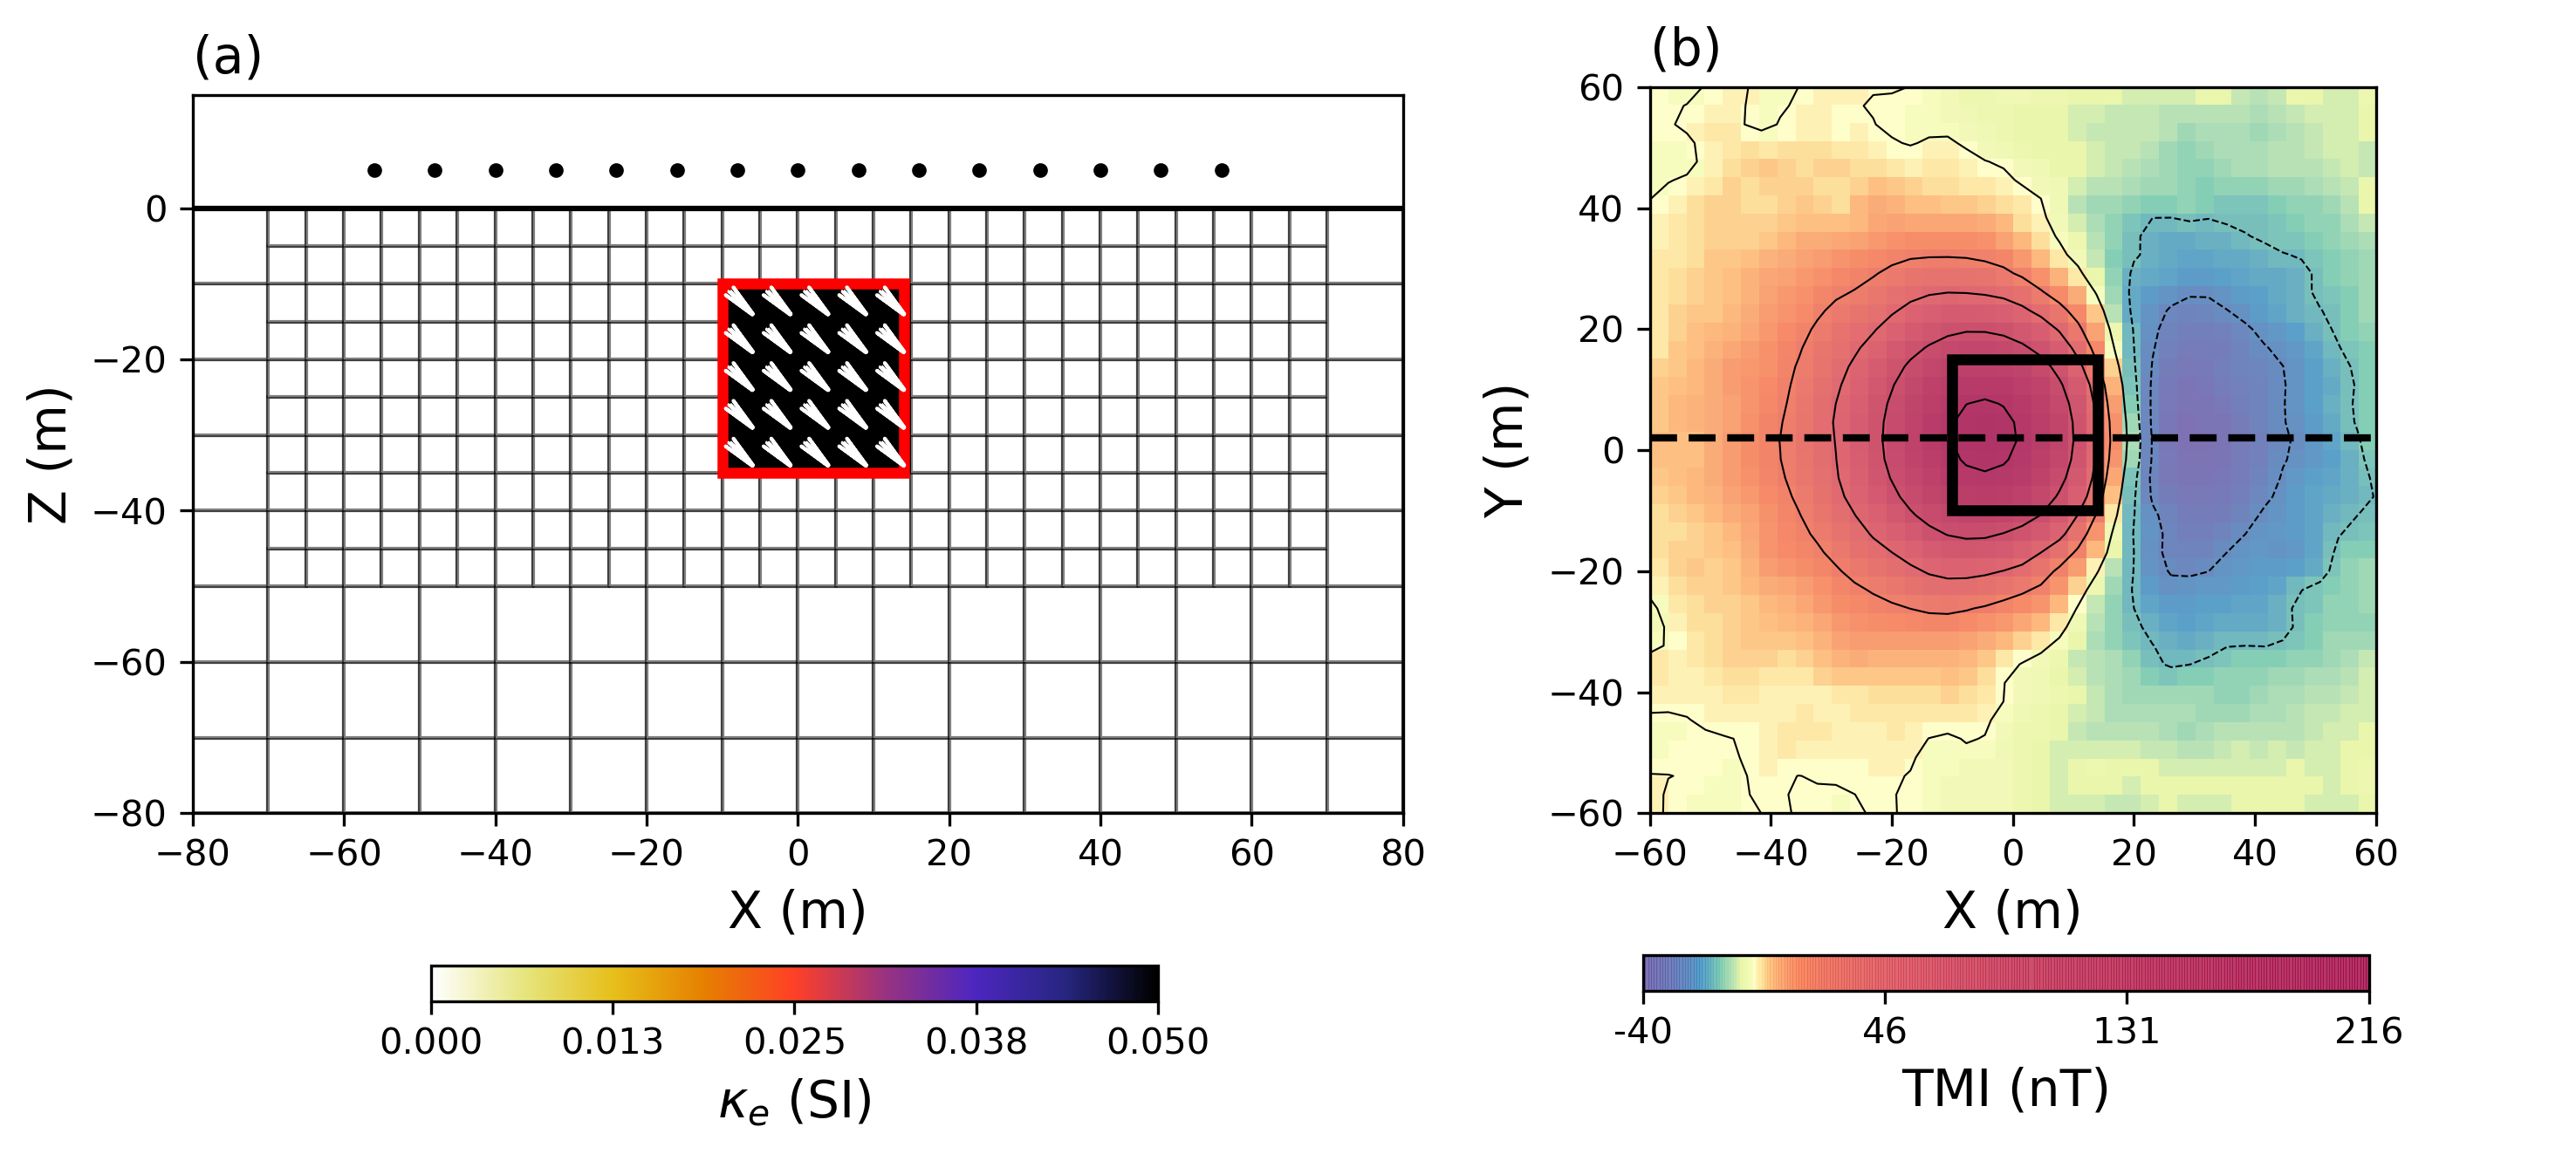
\includegraphics[width=\columnwidth]{Figures/Figure1.png}
\caption{(a) Vertical section through the synthetic block model (Y = 0 m) with magnetization $\mathbf{M}$ [$2.0\: A/m,\; I: 45^\circ,\; D: 90^\circ$]($\kappa_e$ = 0.05 SI). Survey points (black dots) are placed 15 m above the magnetic anomaly. (b) Simulated TMI data map with random Gaussian noise added, 1 nT standard deviation. The horizontal position of the block is shown in black for reference.}
\label{REM_model}
\end{figure}

Since we are dealing with strictly positive magnetic susceptibility $\kappa$, we impose bounds by the projected gradient method \cite[~p.~157]{Vogel02} and use a Gauss-Newton method to solve the inverse problem.
A gradient descent direction $\delta \mathbf{m}$ is calculated by solving
\begin{equation}\label{GaussNewtStep}
\mathbf{H}\; \delta \mathbf{m} = -\mathbf{g}\;,
\end{equation}
where $\mathbf{g}$ is the gradient in equation 9 of the objective function
\begin{equation}\label{grad}
\begin{split}
\mathbf{g} =\; \mathbf{J}^\top \mathbf{W}_d^\top \mathbf{W}_d \left( \mathbb{F}[\mathbf{m}^{(k-1)}] - \mathbf{d}^{obs}\right)+
\beta \sum_{r = s,x,y,z} \alpha_r \mathbf{D}_r^\top \mathbf{R}_r^\top \mathbf{W}_r^\top \mathbf{W}_r \;\mathbf{R}_r \; \mathbf{D}_r \mathbf{m}^{(k-1)}\;,
\end{split}
\end{equation}
and $\mathbf{H}$ is the approximate Hessian:
\begin{equation}\label{Hessian}
\begin{split}
\frac{\partial^2 \phi}{\partial m^2} \approx \mathbf{H} =\;& \mathbf{J}^\top \mathbf{W}_d^\top \mathbf{W}_d \mathbf{J} + \\
& \beta \sum_{r = s,x,y,z} \alpha_r \mathbf{D}_r^\top \mathbf{R}_r^\top \mathbf{W}_r^\top \mathbf{W}_r \;\mathbf{R}_r \; \mathbf{D}_r \;.
\end{split}
\end{equation}
We use the Conjugate Gradient method \cite[]{HestenesStiefel1952} to solve equation 19.
The model update at the $k^{th}$ iteration is then given by
\begin{equation}
\mathbf{m}^{(k)} = \mathbf{m}^{(k-1)} + \alpha \delta \mathbf{m}
\end{equation}
where the step length $\alpha$ is found by a line-search method \cite[~p.~30]{NocedalWright99}.
The optimization problem is solved for a sequence of $\beta$-values until the data misfit reaches the user-defined tolerance $\eta_{\phi_d}$ defined in equation 10.
Since this problem is linear with respect to the model parameters, the sensitivity matrix simplifies to:
\begin{equation}
\mathbf{J} = \frac{\partial \; \mathbb{F}[\boldsymbol{\kappa}]}{\partial \boldsymbol{\kappa}} = \mathbf{F}
\end{equation}
and does not change as a function of iteration.

We begin with the conventional approach that assumes a smooth model ($p_s$, $p_x$, $p_y$, $p_z = 2$). After reaching the target misfit criteria in equation 10, we recover the susceptibility model shown in Figure~\ref{Susc_model}a. We note that the position of the susceptibility anomaly is shifted to the side of the true block and appears to dip at $45^\circ$ angle towards the west. This is due to the large negative lobe introduced in the data by the remanent component that we have ignored. Attempting to improve the solution by solving for a sparse model ($p_s$, $p_x$, $p_y$, $p_z = 0$) yields the solution presented in Figure~\ref{Susc_model}b. The magnetic anomaly is imaged at the right depth and the vertical extent is better recovered, but the position and shape of the anomaly have not improved. In both cases, the data residual maps (Figure~\ref{Susc_model}c and \ref{Susc_model}d) show correlated signal with the location of negative data. The inversion has difficulty reproducing the negative anomalies using strictly positive susceptibility subject to a vertical inducing field.

\begin{figure}[p!]
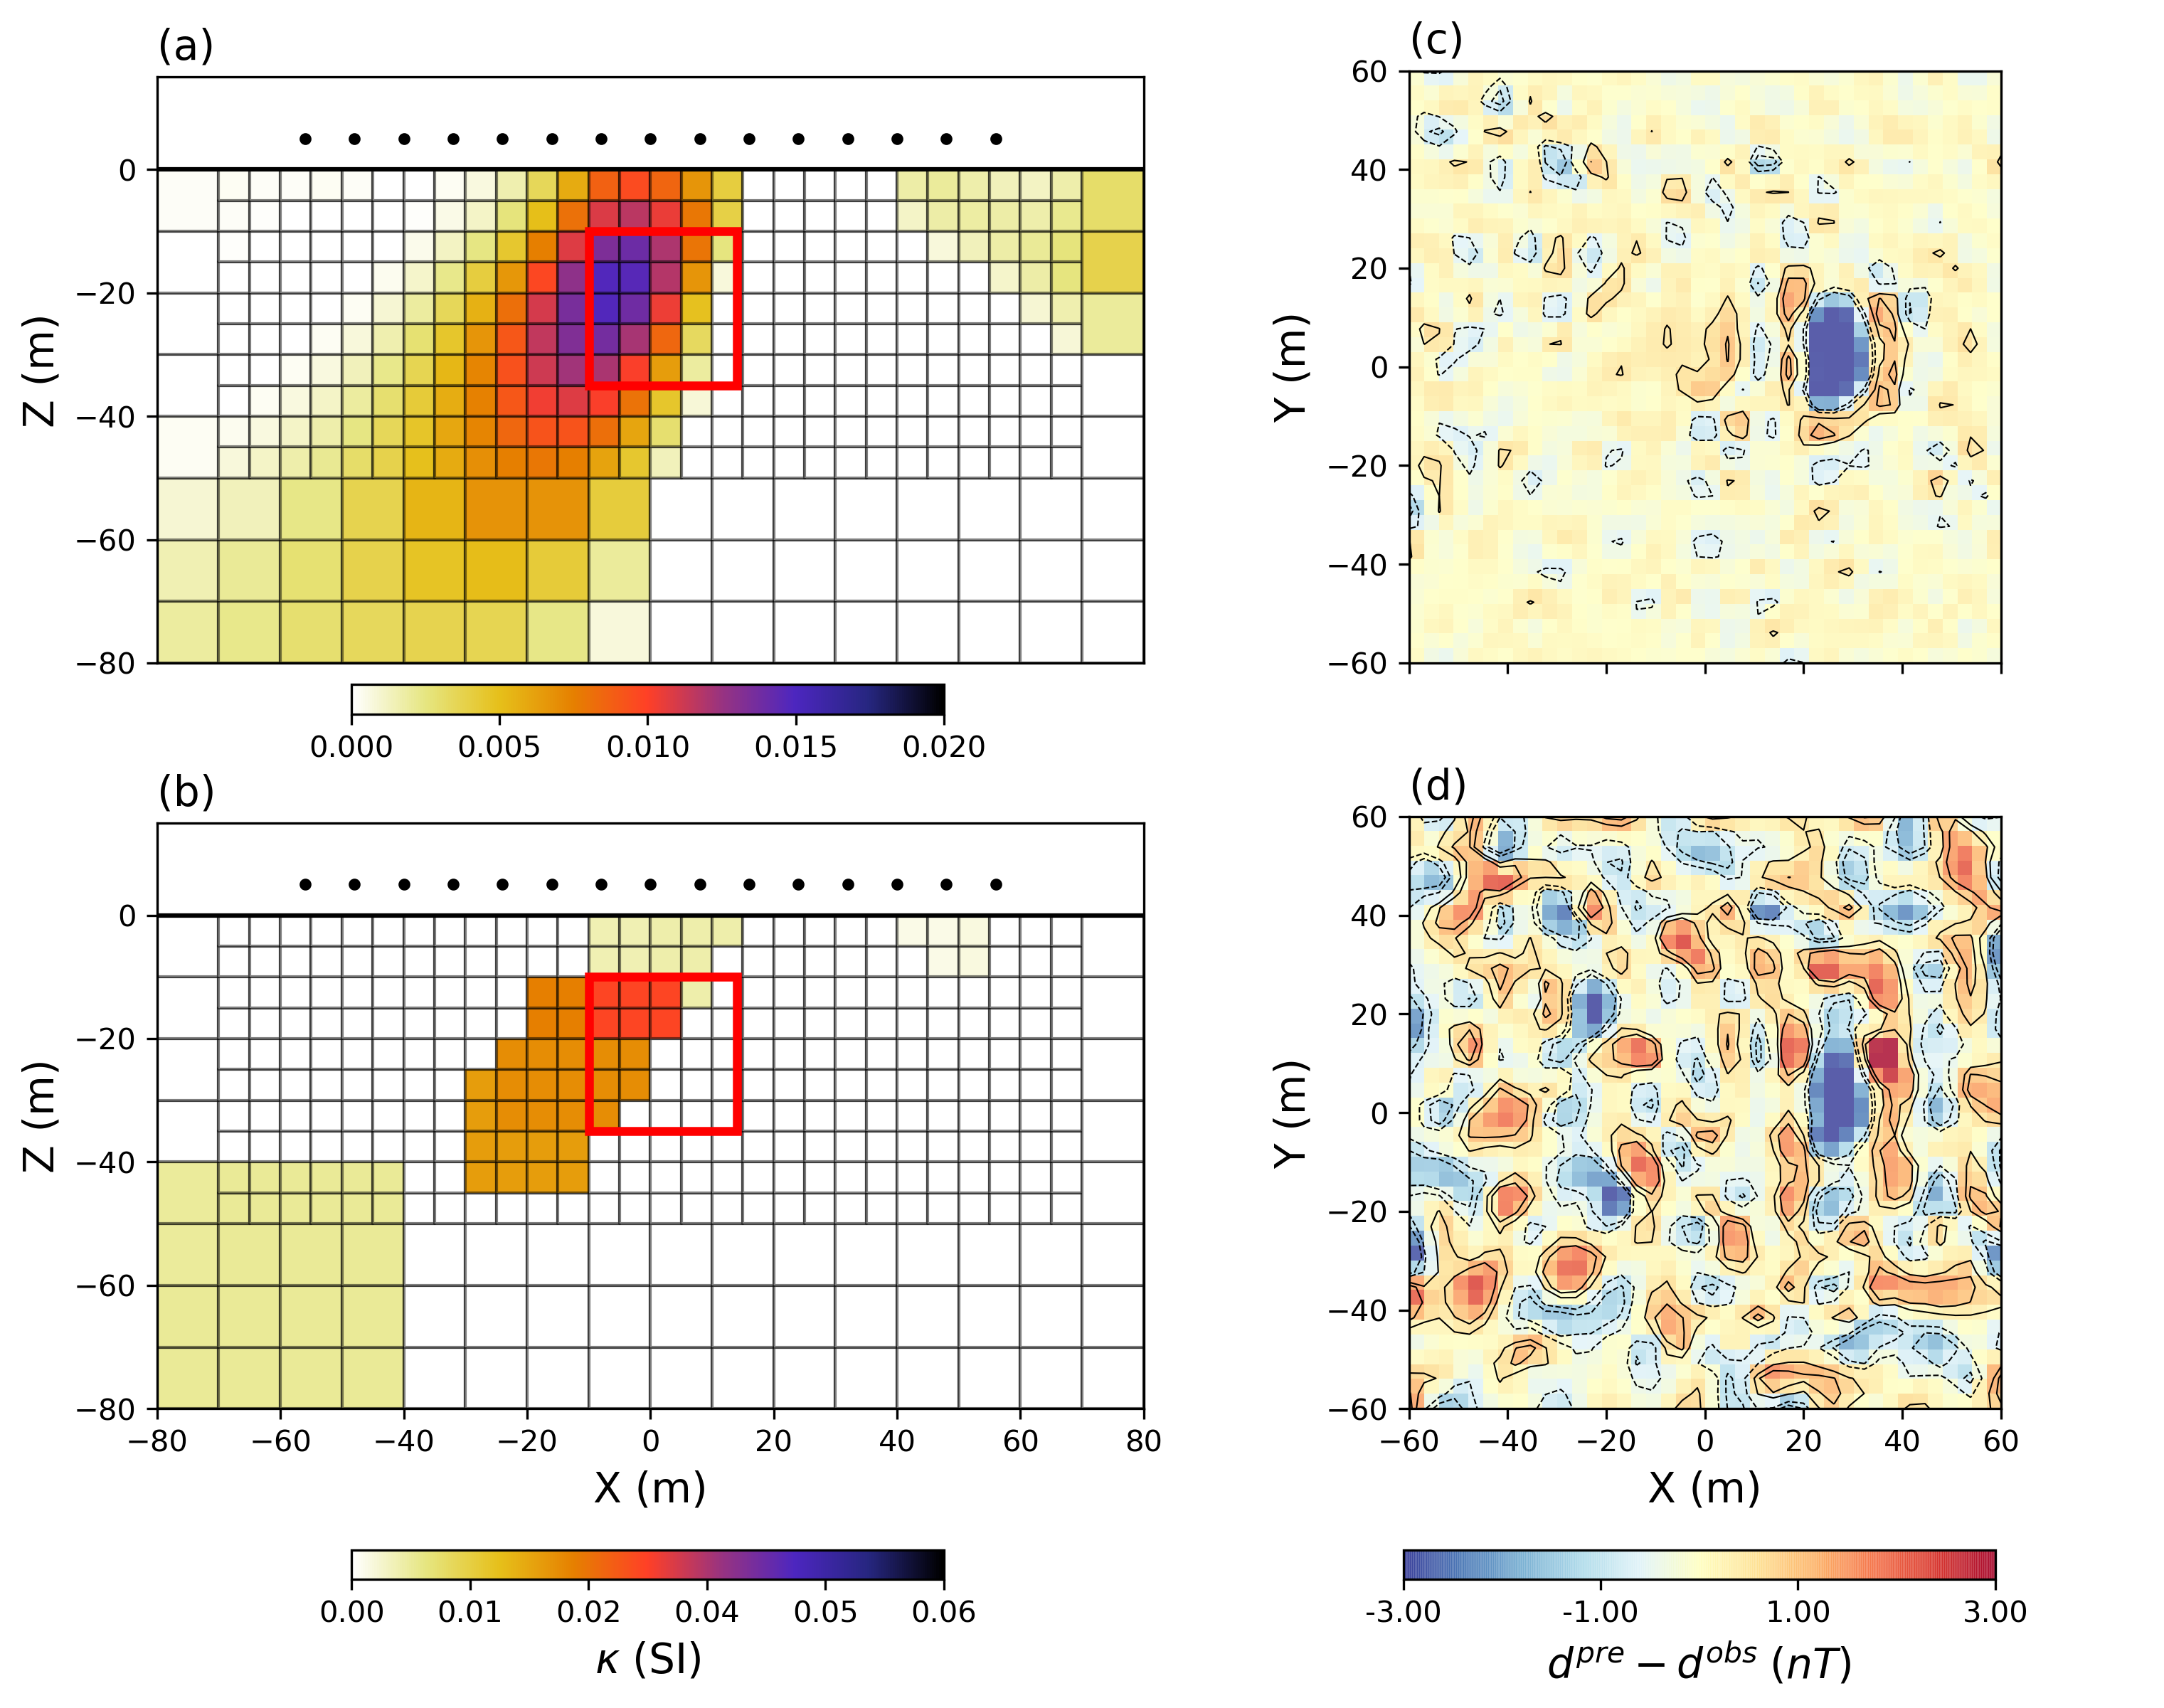
\includegraphics[width=\columnwidth]{Figures/Figure2.png}
\caption{Vertical section through the recovered susceptibility model using (a) smooth assumption ($p_s, \;p_x,\; p_y,\; p_z = 2$) and (b) sparse $\ell_p$-norms to recover a compact model ($p_s,\;p_x,\; p_y,\; p_z = 0$). Both solutions show an anomaly with a false dip due to the wrong assumption of a vertical magnetization. Data residuals for (c) the smooth and (d) compact solution shows correlated signal with the negative data.}
\label{Susc_model}
\end{figure}

The presence of remanence has long been recognized as an obstacle for the geological interpretation of magnetic data.
In a mining exploration context, having the wrong image could result in false drilling targets which is costly in time, resources, and confidence in geophysical methods.
These factors motivate the need for a more robust algorithm that does not require knowledge about the orientation of magnetization.

\subsubsection{Magnetic Vector Inversion - Cartesian parameters}
Generalizing the susceptibility inversion, \cite{LelievreOldenburg2009}
proposed a strategy to directly recover the magnetization vector without assumptions about the orientation. They define an effective susceptibility parameter that scales the strength of magnetization along orthogonal directions such that
\begin{equation}
\vec \kappa_e = \frac{\vec{M}}{\|\vec{h}_0\|} \;.
\end{equation}
Re-writing the discrete system in equation 18 in terms of three orthogonal components of magnetization ($u, v, w$), we obtain the augmented system:
\begin{equation}\label{MVIlinear}
\begin{split}
\mathbf{d}^{pre} &= \mathbf{F}_{e} \boldsymbol{\kappa}_e \\
&= [ \mathbf{F}_u \: \mathbf{F}_v \: \mathbf{F}_w]
\begin{matrix}
\boldsymbol{\kappa}_{u}\\
\boldsymbol{\kappa}_{v}\\
\boldsymbol{\kappa}_{w}
\end{matrix} \\
\mathbf{F}_u,\; &\mathbf{F}_v, \;\mathbf{F}_w \in \mathbb{R}^{N \times M} \;,
\end{split}
\end{equation}
where $\mathbf{F}_u$, $\mathbf{F}_v$ and $\mathbf{F}_w$ are forward operators for the components of magnetization.
We are now dealing with a linear system that has three times the number of unknown parameters compared to the susceptibility assumption ($\boldsymbol{\kappa}_e \in \mathbb{R}^{3M}$). The regularization function in equation 12 becomes
\begin{equation} \label{phi_m_sparse_3C}
\begin{split}
\phi_m = \sum_{c = u,v,w} \;
\sum_{r = s,x,y,z} \alpha_{c_r} {\|\mathbf{W}_r \;\mathbf{R}_{c_r} \; \mathbf{D}_{c_r} \;\mathbf{P}_{c} \; \boldsymbol{\kappa}_e\|}^2_2 \;,
\end{split}
\end{equation}
where the projection matrices $\mathbf{P}_{c}$ select individual components of the vector model $\boldsymbol{\kappa}_e$. Our regularization is made up of 12 terms. Norm measures can be applied to each Cartesian component independently.

Keeping the same inversion methodology and smooth assumptions ($p_{c_s}, \;p_{c_x},\; p_{c_y},\; p_{c_z} = 2$), we recover the magnetization model presented in Figure~\ref{MVI_C_model}a.
This solution is an improvement over the susceptibility inversion as the bulk magnetization is recovered at the right position and with the correct magnetization orientation on average inside the block. We note however that the solution is distributed over a large volume and with a broad distribution in magnetization direction.

\begin{figure}[p!]
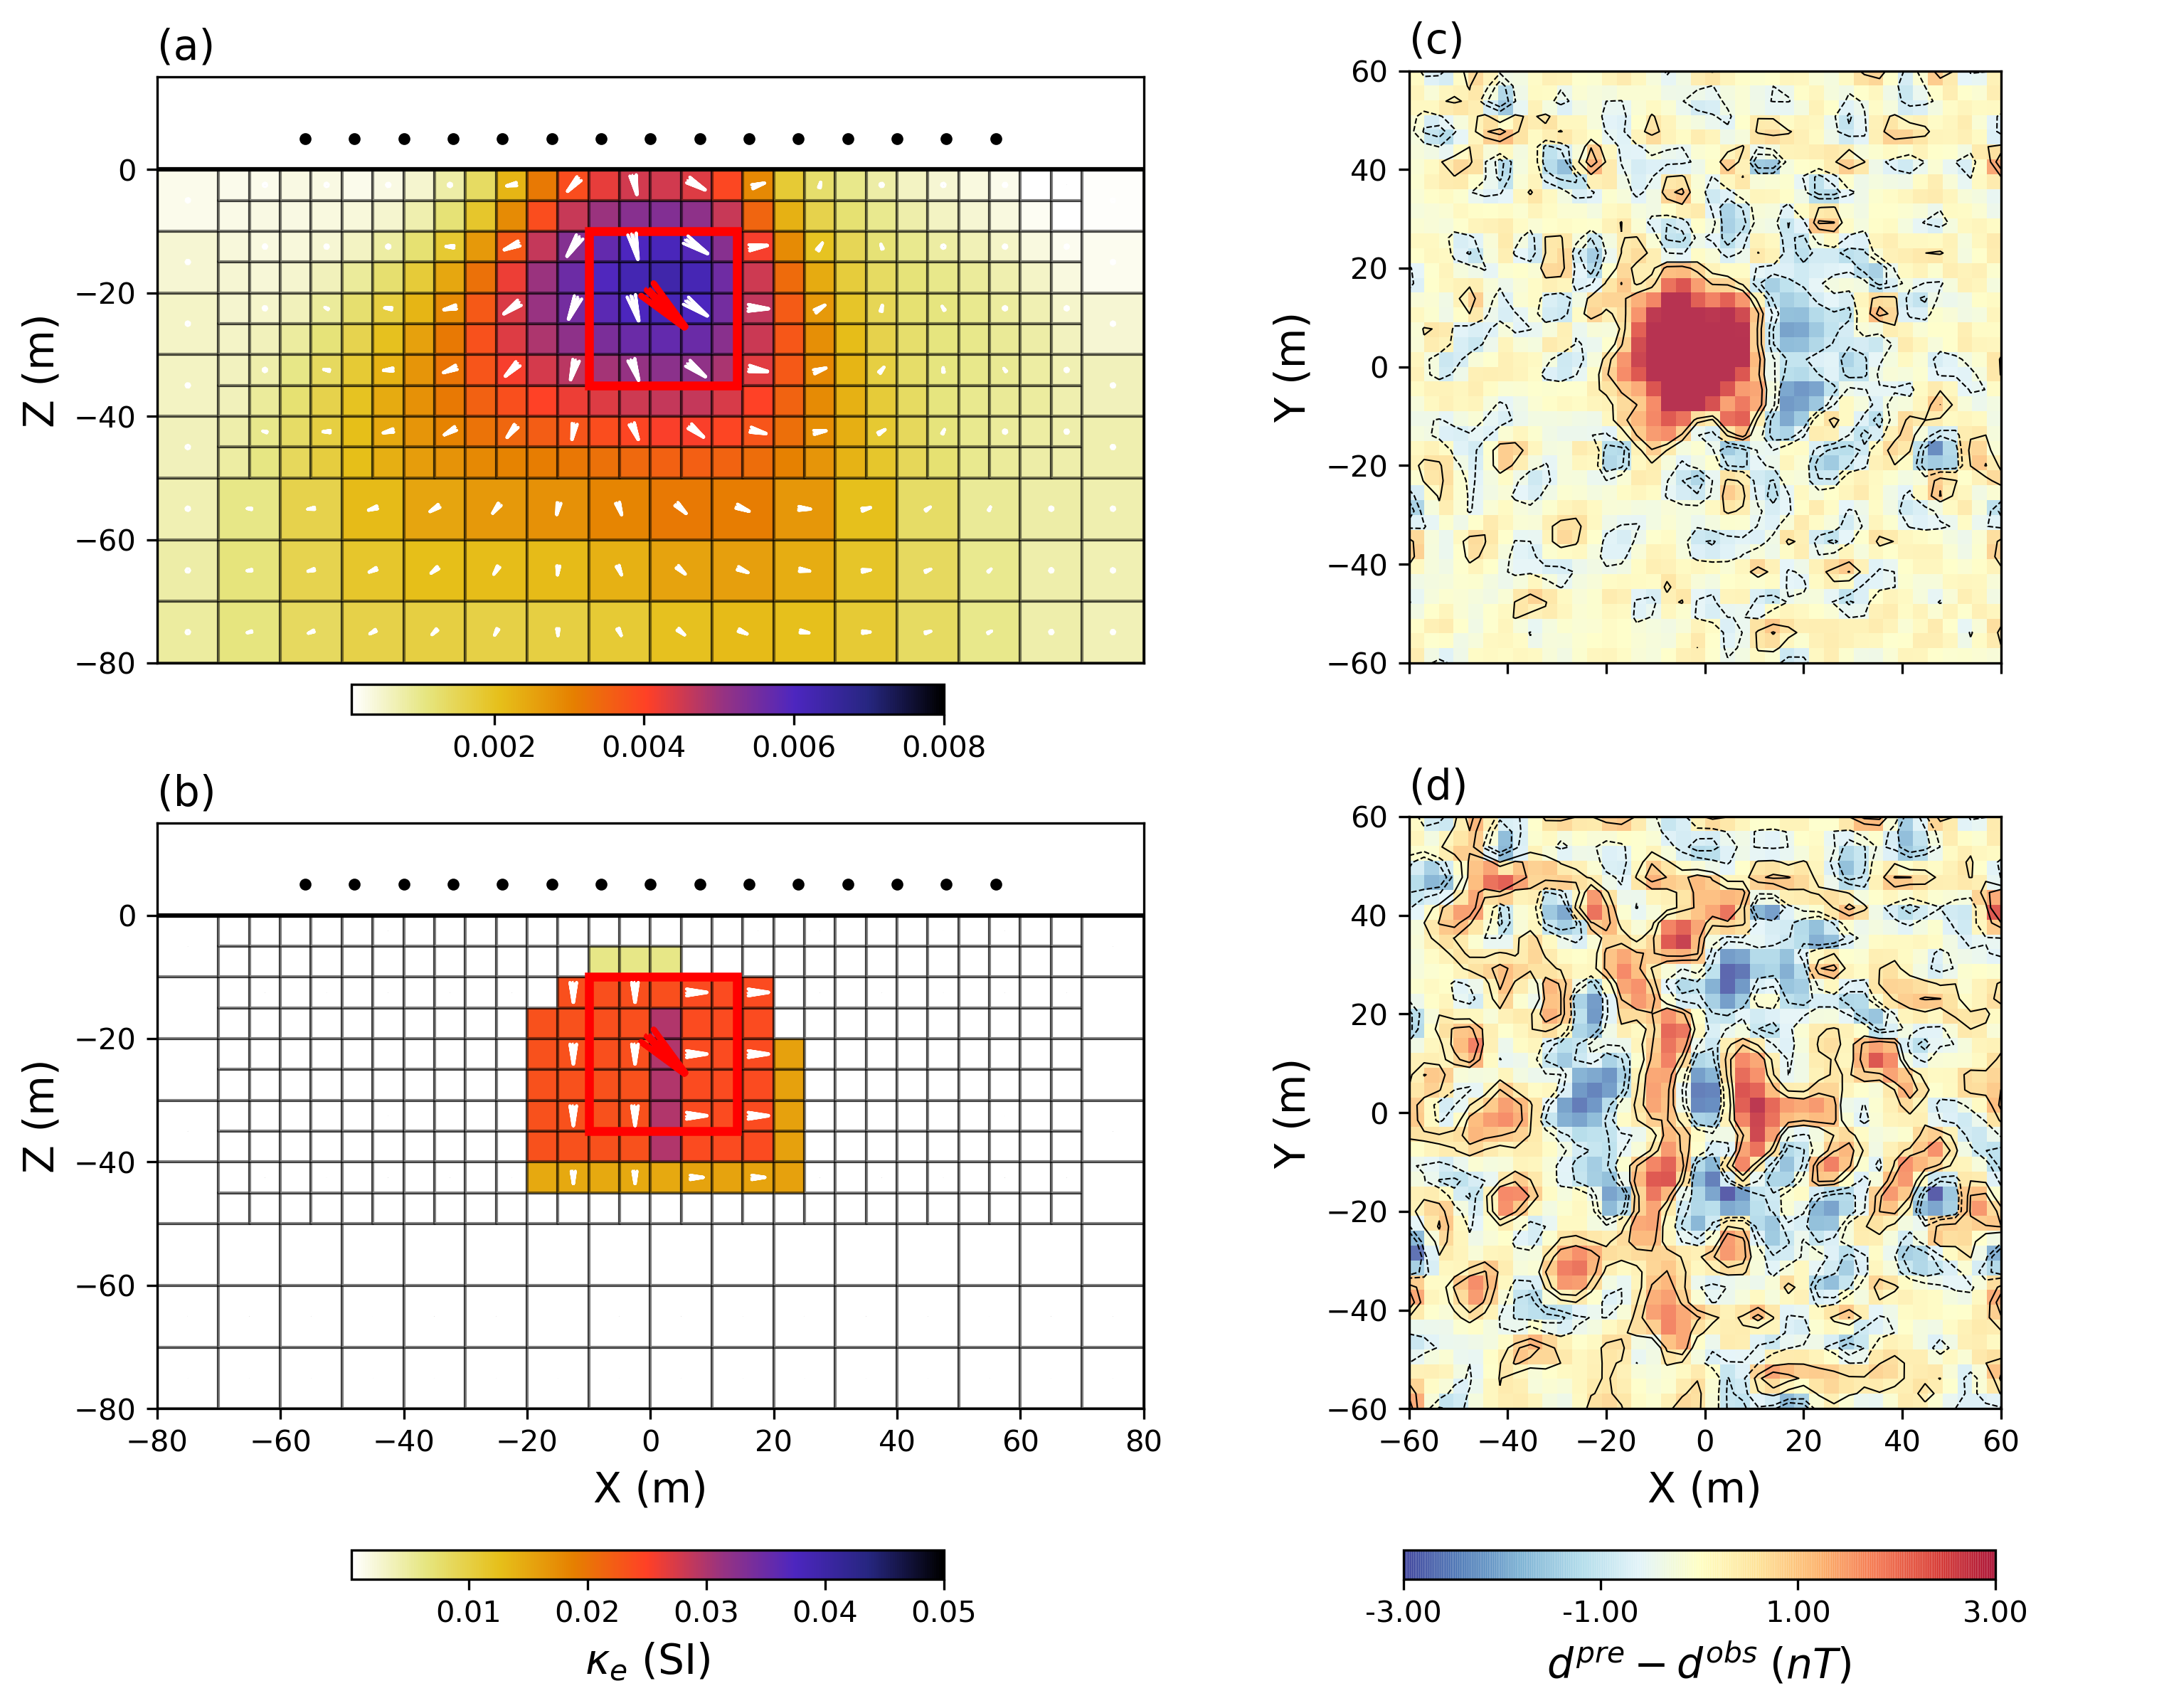
\includegraphics[width=\columnwidth]{Figures/Figure3.png}
\caption{Vertical section through the recovered magnetization vector model using the Cartesian formulation with (a) smooth $l_2$-norm assumption and (b) sparsity constraints applied on all three Cartesian components ($p_{i_s}, \;p_{i_x},\; p_{i_y},\; p_{i_z} = 0$). Color is scaled by the magnitude of magnetization. The true magnetization direction is shown with a red arrow. Data residual map calculated with (c) the smooth and (d) compact solution.}
\label{MVI_C_model}
\end{figure}

In order to reduce the complexity of the solution, we once again resort to the $\ell_p$-norm measure ($p_{c_s}, \;p_{c_x},\; p_{c_y},\; p_{c_z} = 0$). As shown in Figure~\ref{MVI_C_model}b, the recovery of the block has clearly improved. It is important to point out, however, that the magnetization vectors are pointing along the Cartesian directions and the anomaly is slightly wider than the true model. In the Cartesian formulation, both the direction and strength of magnetizations are coupled in the vector components. This formulation therefore lacks flexibility in recovering sparse vector along arbitrary orientations. This was the main motivation behind recent research investigating more advanced regularization methodologies \cite[~p.~101]{Zhu2015, Liu2015, Fournier2015}. We will attempt to improve this solution by decoupling the strength and direction of the magnetization vector with the spherical formulation.

\subsubsection{Magnetic Vector Inversion - Spherical parameters}
As an alternative to the Cartesian formulation, \cite{LelievreOldenburg2009} also proposed the vector inversion in a spherical coordinate system.
The conversion between Cartesian to spherical system follows the relation:
\begin{equation}\label{eq:Cart_to_Spherical}
\begin{split}
u = & \rho \; \cos(\theta)\;\cos(\phi) \\
v = & \rho \; \cos(\theta)\;\sin(\phi) \\
w = & \rho \; \sin(\theta)
\end{split}
\end{equation}
where the magnetization vector is defined by parameters of amplitude (${\rho}$) and two angles (${\theta}$, ${\phi}$).
The spherical formulation separates the magnitude and orientation of magnetization vector, which comes with two advantages. First, physical property constraints from rock measurements (Koenigsberger ratio, magnetization angle) can easily be incorporated. Second, sparsity constraints can be applied to the magnitude and orientation independently, potentially resulting in compact bodies with uniform magnetization direction in any orientation.

Despite its obvious advantages, the MVI-S method has received little attention in the literature due to the non-linear transformation it introduces.
We demonstrate challenges encountered with the spherical approach on our synthetic problem.
Taking the partial derivatives of equation 25 as a function of $\mathbf{m}( \boldsymbol{\rho}, \boldsymbol{\theta}, \boldsymbol{\phi})$ yields:
\begin{equation} \label{eq:spherical}
\mathbf{J} = \frac{\partial \mathbf{F}_{e}[\boldsymbol{\kappa}_e]}{\partial \mathbf{m}} = \frac{\partial \mathbf{F}_{e}[\boldsymbol{\kappa}_e]}{\partial \boldsymbol{\kappa}_e} \frac{\partial \boldsymbol{\kappa}_e}{\partial \mathbf{m}}\;,
\end{equation}
where $\frac{\partial \mathbf{k}_e}{\partial \mathbf{m}}$ involves partial derivatives of trigonometric functions prescribed in equation 27.
The sensitivity matrix can be linearized before each Gauss-Newton step as:
\begin{equation} \label{eq:lin_sph}
\mathbf{J} = \mathbf{F}_{e}\: \mathbf{S}\;,
\end{equation}
where the matrix $\mathbf{S}$ holds the partial derivatives
\begin{equation} \label{eq:Smatrix}
\mathbf{S} = \begin{bmatrix} \cos{\theta}\cos{\phi} & -\rho\sin{\theta}\cos{\phi} & -\rho\cos{\theta}\sin{\phi} \\
\cos{\theta}\sin{\phi} & -\rho\sin{\theta}\sin{\phi} & \rho\cos{\theta}\cos{\phi} \\
\sin{\theta} & \rho\cos{\theta} & 0 \end{bmatrix}\;.
\end{equation}
With this choice of parameterization, the regularization function becomes
\begin{equation} \label{phi_m_sparse_Spherical}
\begin{split}
\phi_m = \sum_{c = \rho,\theta,\phi} \;
\sum_{r = s,x,y,z} \alpha_{c_r} {\|\mathbf{W}_r \;\mathbf{R}_{c_r} \; \mathbf{D}_{c_r} \;\mathbf{P}_{c} \; \mathbf{m}\|}^2_2 \;.
\end{split}
\end{equation}
We note that zero reference angle values $\boldsymbol \theta_{ref}$ and $\boldsymbol \phi_{ref}$ would imply a magnetization direction pointing along the $x$-axis. Since we do not want to assume a specific orientation (no ground truth), we set $\alpha_{\theta_s}=\alpha_{\phi_s} = 0$ in all our experiments such that the regularization only penalizes the change in angle between neighboring cells.

To demonstrate the difficulties that the nonlinearity of the MVI-S formulation can cause in the inversion, we invert our synthetic TMI data with the wrong initial assumption $\mathbf{m_0}(\rho=10^{-2}, \theta=-45^{\circ}, \phi=0^{\circ}$), such that the starting magnetization orientation is  $90^\circ$ from the true model (Figure~\ref{MVI_S_model_noScale}a). After convergence of the algorithm, we recover the model shown in Figure~\ref{MVI_S_model_noScale}b. The solution is a poor representation the true magnetization. Model updates were forced to stop before reaching the target data misfit and the optimization is likely trapped in a local minimum. We note that most of the model updates were performed on the amplitude $\rho$, with only marginal changes on the angle of magnetization. Similar behaviors have been documented by \cite{LelievreOldenburg2009} and later by \cite{Liu2017}, who attributed  the problem to an imbalance between the model parameters. Before attempting to implement more advanced constraints, we make improvements to the convergence of the non-linear MVI-S formulation.

\begin{figure}[p!]
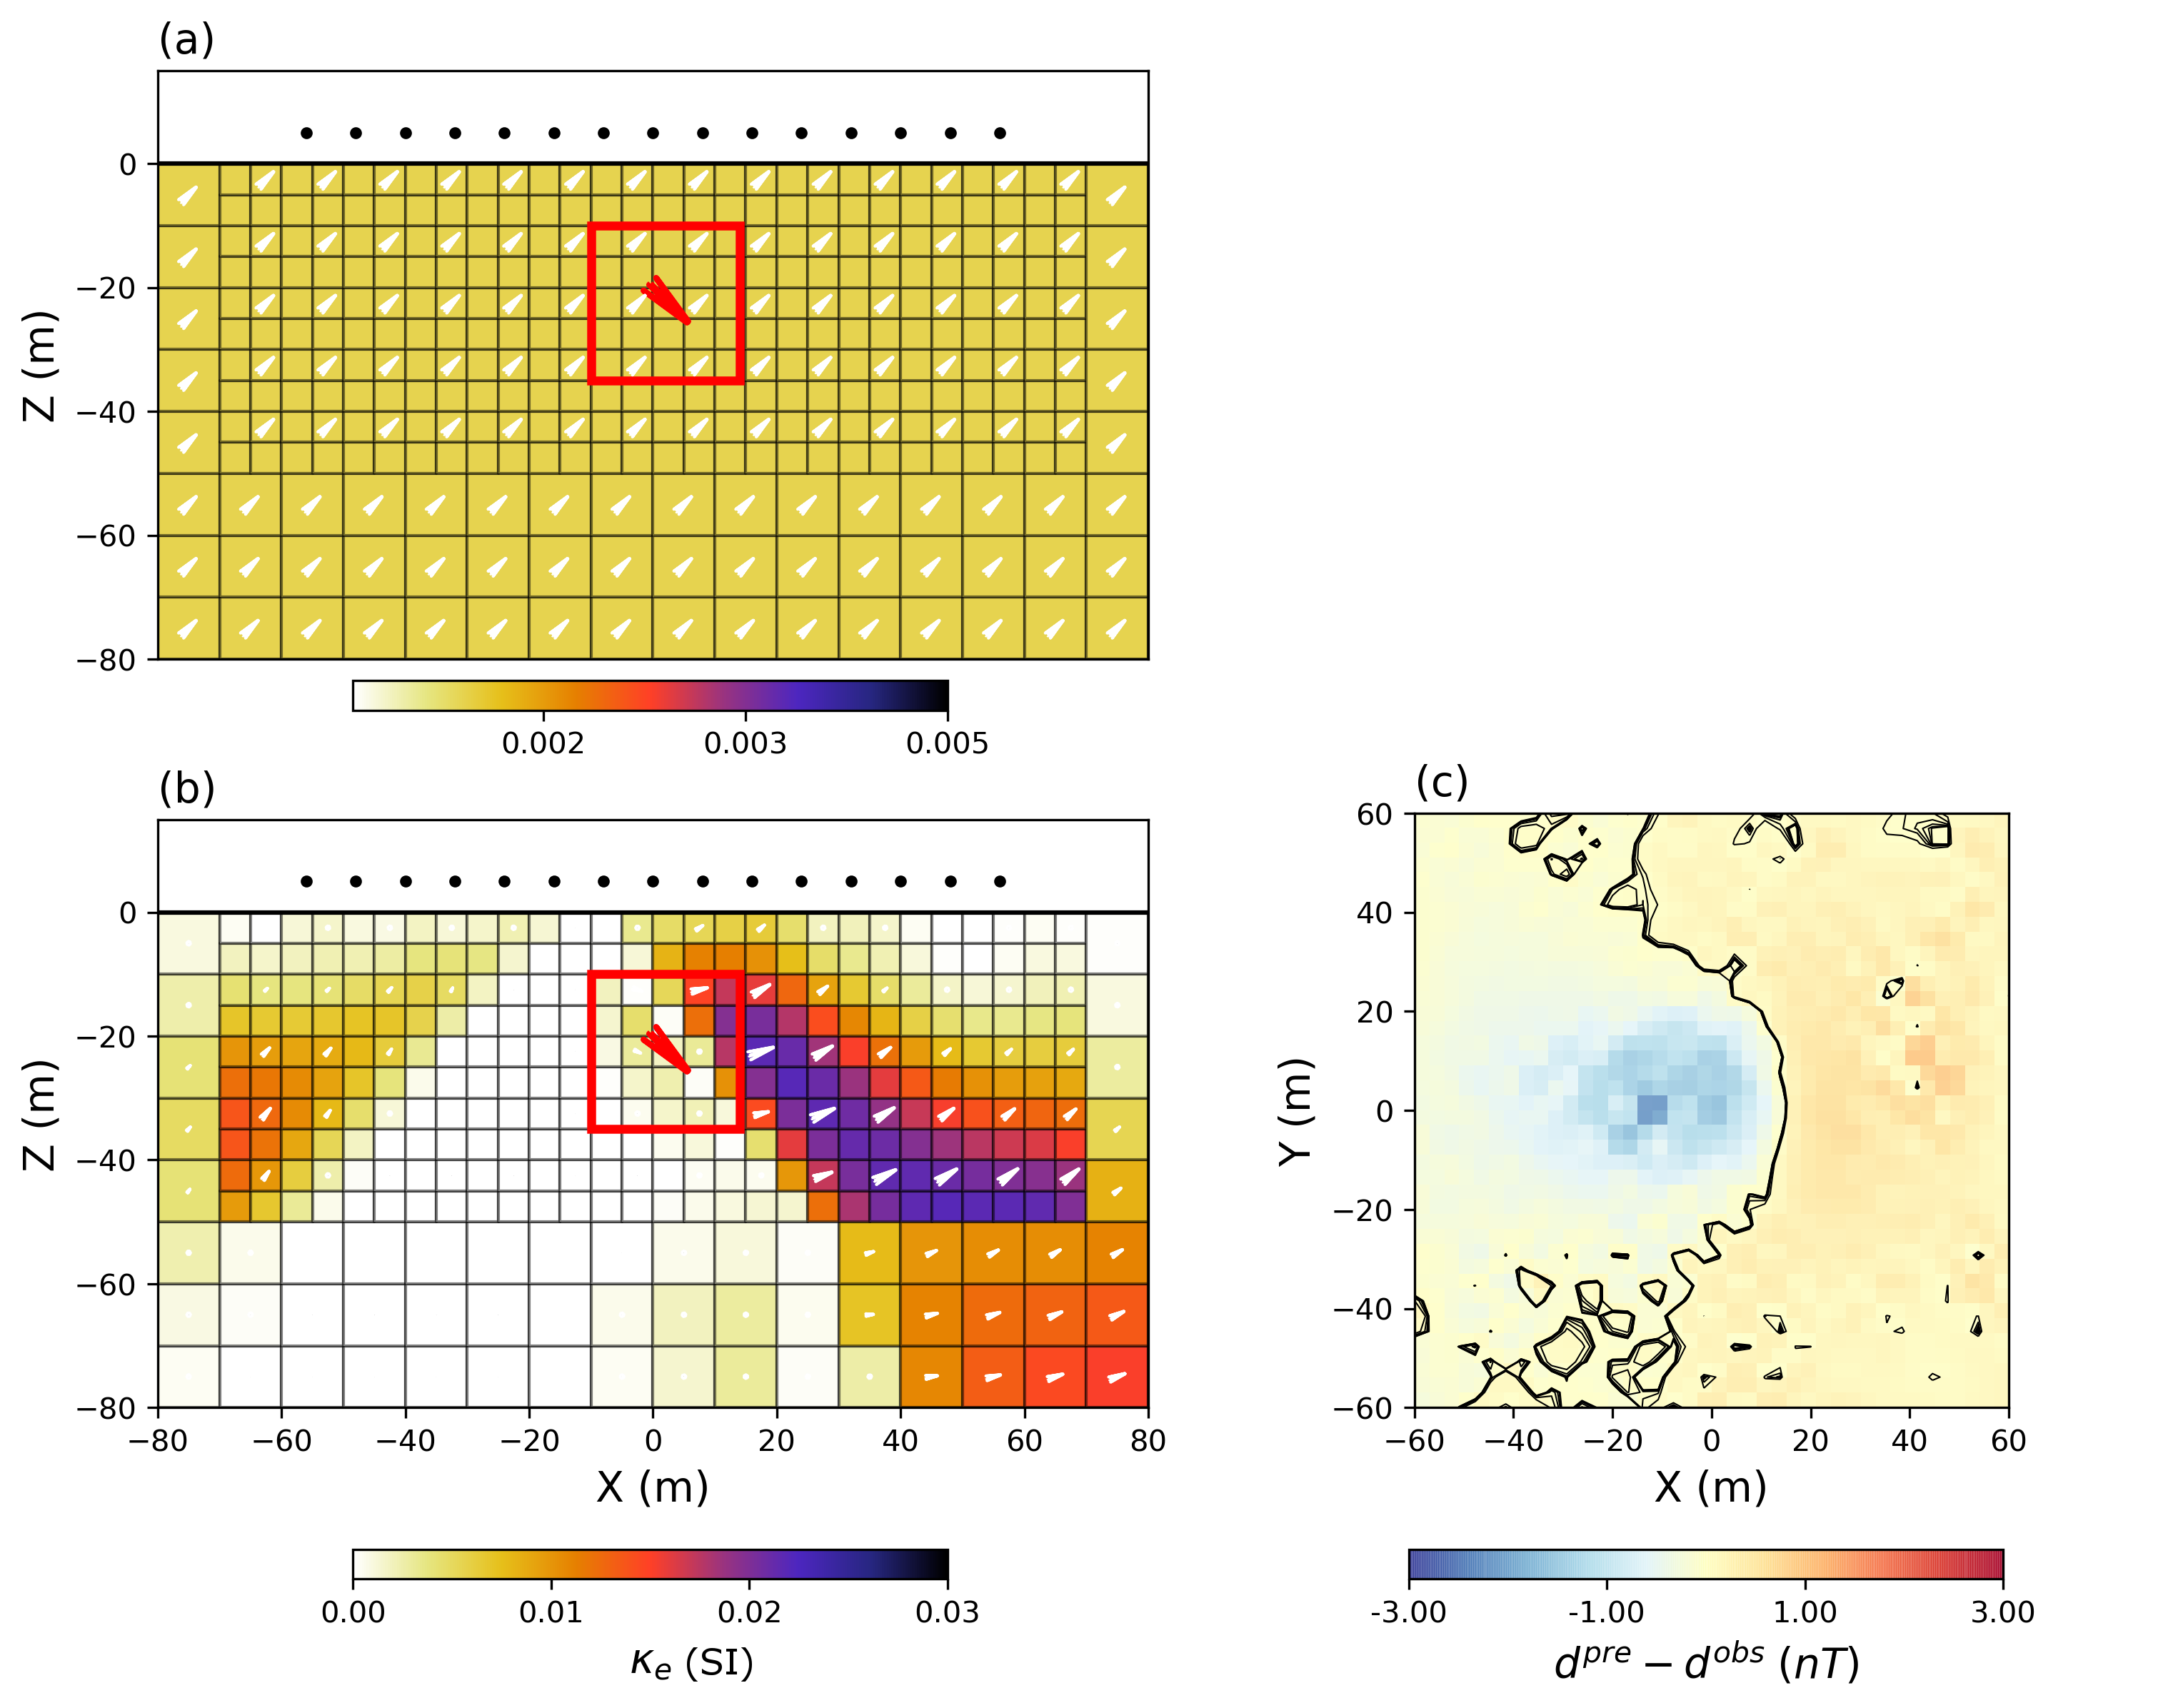
\includegraphics[width=\columnwidth]{Figures/Figure4.png}
\caption{ Vertical section through the (a) starting model and (b) recovered magnetization vector model in spherical coordinates with its (c) data residual map. The inversion stopped after three iterations, unable to further reduce the objective function.}
\label{MVI_S_model_noScale}
\end{figure}

\subsection{Iterative sensitivity re-weighting}
To gain some insight about the issues encountered with the MVI-S formulation, we consider a simpler two-parameter linear problem of the form
\begin{equation}
x + \:2\:y =1 \;,
\end{equation}
which we can express in matrix form as
\begin{equation}\label{twoParam}
\begin{split}
\mathbf{F}_C\;\mathbf{m}_C &= \mathbf{d}^{obs} \;,\\
\mathbf{F}_C = [1\;2], \;
\mathbf{m}_C &=
\begin{matrix}
x\\
y
\end{matrix}, \;
\mathbf{d}^{obs} = 1
\end{split}
\end{equation}
This defines an under-determined linear system of equations. Just as we did for the magnetic inverse problem, we can isolate a solution by minimizing an objective function of the form
\begin{equation}\label{toyProblem}
\phi(m) = \| \mathbf{F}_C\;\mathbf{m}_C - \mathbf{d}^{obs} \|_2^2 + \beta_C \| \mathbf{m}_C \|_2^2 \;.
\end{equation}
Figure~\ref{NonLinearGN}a displays a contour map of the objective function along with its gradients.

\begin{figure}[p!]
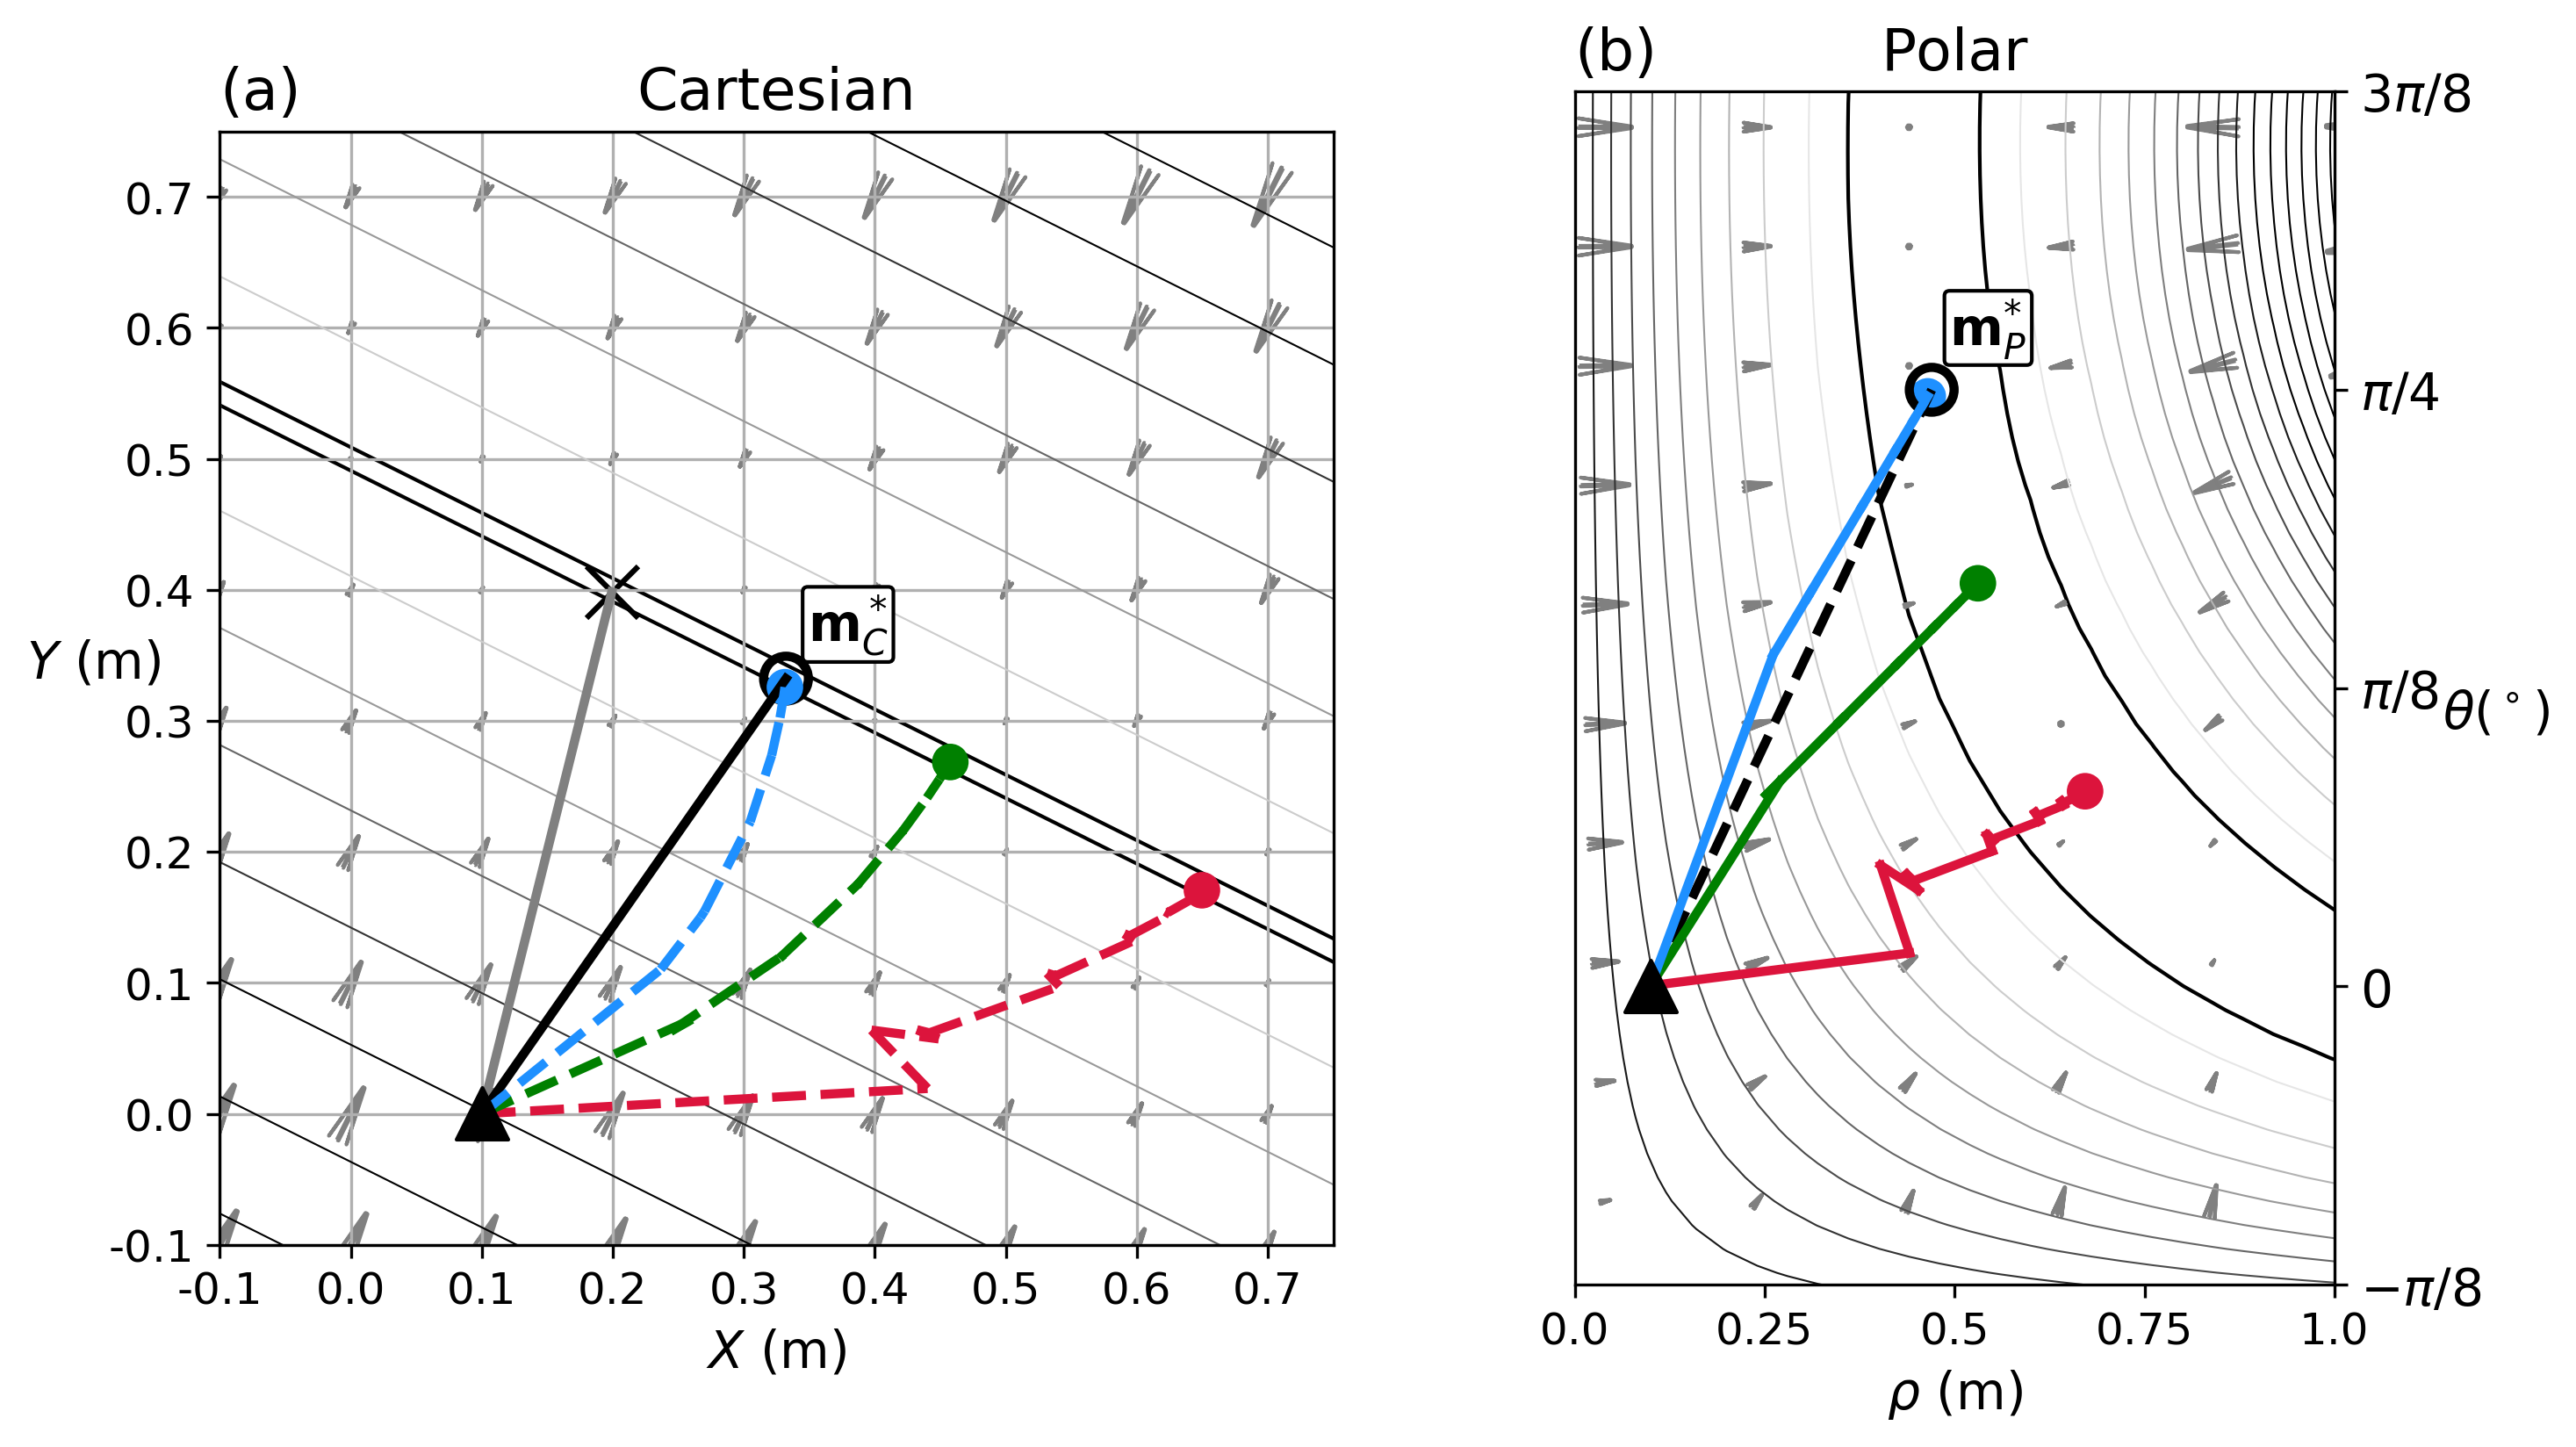
\includegraphics[width=\columnwidth]{Figures/Figure5.png}
\caption{Contour maps for the objective functions of a two-parameter inverse problem solved in (a) Cartesian and (b) polar coordinate systems. Solid colored lines show the model updates taken by different algorithms in their respective coordinate systems and, in dash, the equivalent steps in the other domain for comparison. Each inversion started with the same initial model (triangle). The colors and inversions are: Gray: the non-weighted Cartesian problem; Black: the sensitivity weighted Cartesian problem; Red: the non-linear polar coordinate system with fixed sensitivity weights; Green: the polar problem with iterative sensitivity re-weighting; and Blue: with the added scaling to compensate for the dynamic range of the parameters (see equation~50). }
\label{NonLinearGN}
\end{figure}

Following the same methodology as in equation 9, we find a solution such that the gradient of the objective function $\phi(m)$ vanishes
\begin{equation}\label{gradLinear}
\begin{split}
\frac{\partial \phi}{\partial \mathbf{m}}=\mathbf{g} = \left(\mathbf{F}_C^\top\mathbf{F}_C + \beta_C \mathbf{I}\right) \mathbf{m}_C - \mathbf{F}_C^\top \mathbf{d}^{obs} &= \mathbf{0}\;,
\end{split}
\end{equation}
where $\mathbf{I}$ is the identity matrix. The factor of 2 from the derivative of the $\ell_2$-norm is absorbed by the zero right-hand side.
After determining a trade-off parameter $\beta_C$ such that $\phi_d \leq 10^{-3}$, we recover the Cartesian model $\mathbf{m}_C[x=0.2, y=0.4]$. It is the solution that minimizes the distance (evaluated with the $\ell_2$-norm) between the origin and the solution space of $\mathbf{F}_C$. We note that the relative magnitudes of model parameters in $\mathbf{m}_C$ reflect the size of the forward coefficients in $\mathbf{F}_C$.


As previously discussed for the magnetic problem, the smallest solution is often not satisfactory as it is strongly influenced by the physics of the experiment.
From equation 15, we can introduce sensitivity-based weights to counteract this bias towards a large $y$ value:
\begin{equation}
\begin{split}
\mathbf{W}_C &= \rm{diag} \left[ {\left[\frac{\mathbf{ w}_C}{\rm{max}(\mathbf{ w}_C)}\right]}^{1/2}\right]\\
w_{C_j} &= {\left[\sum_{i=1}^{N}{F_{ij}}^2 \right]}^{1/2}\;,
\end{split}
\end{equation}
where $\mathbf{W}_C$ holds sensitivity weights added to the regularization ($\mathbf{w}_C=[1,\:2]^\top$).
The new weighted objective function becomes
\begin{equation}\label{toyProblem}
\phi(m) = \| \mathbf{F}_C\;\mathbf{m}_C - \mathbf{d}^{obs} \|_2^2 + \beta_C \| \mathbf{W}_C \mathbf{m}_C \|_2^2 \;,
\end{equation}
and the weighted gradient is
\begin{equation}\label{gradLinearWeighted}
\begin{split}
\mathbf{g}_C = \mathbf{F}_C^\top\mathbf{F}_C \mathbf{m}_C + \beta_C \mathbf{W}_C^\top\mathbf{W}_C\mathbf{m}_C - \mathbf{F}_C^\top \mathbf{d}^{obs}\;.
\end{split}
\end{equation}
After determining the appropriate $\beta_C^*$, we get the solution $\mathbf{m}^*_C[x=0.33, y=0.33]$ marked with a black circle in Figure~\ref{NonLinearGN}a. We have reached the only solution with equal contribution from both model parameters that also predicts the data within the tolerance.

Alternatively, we can attempt to solve the same problem in a polar coordinate system under the transformation
\begin{equation}
\begin{split}
	\mathbf{m}_P &= [\rho,\;\theta]^\top\\
	x &= \rho \cos{\theta} \\
	y &= \rho \sin{\theta} \;,\\
\end{split}
\end{equation}
where the polar model $\mathbf{m}_P$ is defined by a radius $\rho$ and an angle $\theta$. This is analogous to the spherical transformation performed for the MVI-S formulation in equation 27.
The objective function to be minimized becomes
\begin{equation}\label{toyPolar}
\begin{split}
\phi(\mathbf{m}_P)= \| \mathbb{F}[\mathbf{m}_P] - \mathbf{d}^{obs} \|_2^2 + \beta_P \| \mathbf{W}_C \mathbf{m}_P \|_2^2 \;.
\end{split}
\end{equation}
The inverse problem is now non-linear with respect to the polar model so we solve it iteratively with the standard Gauss-Newton procedure described in equation 19.
The partial derivatives of the forward mapping with respect to the polar coordinates are calculated by
\begin{equation}\label{Jpolar}
\begin{split}
\mathbf{J} = \frac{\partial \mathbb{F}[\mathbf{m}_P]}{\partial \mathbf{m}_P} &= \frac{\partial \mathbb{F}[\mathbf{m}_P]}{\partial \mathbf{m}_C} \frac{\partial \mathbf{m}_C}{\partial \mathbf{m}_P} = \mathbf{F}_C\mathbf{S} \\
\end{split}
\end{equation}
where the matrix $\mathbf{S}$ holds the partial derivatives of the model with respect to the polar parameters
\begin{equation}\label{nonlinF}\begin{split}
\mathbf{S} &=
\begin{bmatrix}
\cos{\theta} & -\rho\sin{\theta} \\
\sin{\theta} & \rho\cos{\theta}
\end{bmatrix} \;.
\end{split}
\end{equation}
The gradient of the objective function becomes
\begin{equation}\label{gradPolar}
\begin{split}
\mathbf{g}_P = \mathbf{S}^\top \mathbf{F}_C^\top \:\mathbb{F}[\mathbf{m}_P] + \beta_P \mathbf{W}_C^\top\mathbf{W}_C \mathbf{m}_P - \mathbf{S}^\top \mathbf{F}_C^\top \mathbf{d}^{obs} \;.
\end{split}
\end{equation}
A trade-off parameter $\beta_P$ is determined through the cooling schedule established previously. The inversion is terminated once the data misfit falls below the tolerances $\eta_{\phi_d}$ defined in equation 10.

Since $\mathbf{m}_C^*\;[x=0.33, y=0.33]$ is a desirable model, we would like to be able to recover a similar solution in polar parameters ($\mathbf{m}_P^{*}[\rho=0.47, \theta=0.76]$). Unfortunately, as shown in Figure~\ref{NonLinearGN}b, the minimization process performed in polar coordinates converges to a different solution ($\mathbf{m}_P\;[ \rho=0.67,\:\theta=0.26]$) and the iterations steps are oscillatory.
We display the equivalent iterations (red dash) in the Cartesian space for comparison ($\mathbf{m}_C^P\;[ x=0.65,\:y=0.17]$). This is an unsatisfactory solution.

Our main goal is to recover the solution $\mathbf{m}_P^{*}$, and we want to reach it with only a few model updates.
To understand  why the problem has arisen we compare their respective gradients for a given starting model $\mathbf{m}_C^{(0)}$ and its equivalent polar model $\mathbf{m}_P^{(0)}$. In Cartesian coordinates, the gradient direction is
\begin{equation}\label{gradC_0}
\begin{split}
\mathbf{g}_C^{(0)} = \mathbf{F}_C^\top \:\mathbf{F}_C\mathbf{m}_C^{(0)} + \beta_C \mathbf{W}_C^\top\mathbf{W}_C \mathbf{m}_C^{(0)} - \mathbf{F}_C^\top \mathbf{d}^{obs}\;. \\
\end{split}
\end{equation}
We can convert these gradients to polar coordinate by multiplying equation 44 with the matrix of partial derivatives $\mathbf{S}$ such that
\begin{equation}\label{gradCtoP}
\begin{split}
\mathbf{g}_P^C = \mathbf{S}^\top \left[ \mathbf{F}_C^\top \:\mathbf{F}_C\mathbf{m}_C^{(0)} + \beta_C \mathbf{W}_C^\top\mathbf{W}_C \mathbf{m}_C^{(0)} - \mathbf{F}_C^\top \mathbf{d}^{obs} \right] \;.\\
\end{split}
\end{equation}
We want to compare this gradient to the gradient calculated in polar coordinates. From equation 43, and also keeping the same $\beta_C$ used in the Cartesian framework, we have
\begin{equation}\label{gradP}
\begin{split}
\mathbf{g}_P &= \mathbf{S}^\top \mathbf{F}_C^\top \:\mathbb{F}[\mathbf{m}_P^{(0)}] + \beta_C \mathbf{W}_C^\top\mathbf{W}_C \mathbf{m}_P^{(0)} - \mathbf{S}^\top \mathbf{F}_C^\top \mathbf{d}^{obs}\;.
\end{split}
\end{equation}
Noting that $\mathbf{F}_C \mathbf{m}_C^{(0)} = \mathbb{F}[ \mathbf{m}_P^{(0)}]$ (i.e. the forward modellings are consistent) then equation 45 and 46 are the same only if
\begin{equation}\label{gradientmCvsmPSimple}
\begin{split}
 \mathbf{S}^\top \mathbf{W}_C^\top\mathbf{W}_C \mathbf{m}_C^{(0)} & \simeq  \mathbf{W}_C^\top\mathbf{W}_C \mathbf{m}_P^{(0)}\;.
\end{split}
\end{equation}
We would like both sides to be roughly equal such that the gradient direction in polar space resembles the gradient direction calculated in the Cartesian space. This is unlikely since S is a coordinate transformation matrix whose columns can have quite different values (see equation 42).
The critical element is the specification of the regularization matrix for the polar system. Using the regularization matrix generated for the Cartesian system is inappropriate. Instead, we should use the sensitivity weighting for the polar problem. From equation 41 we had defined the polar sensitivities as $\mathbf{J}=\mathbf{F}_C\mathbf{S}$. We can define a new weighting matrix $\mathbf{W}_P$ by
\begin{equation}
\begin{split}
\mathbf{W}_P &= \rm{diag} \left[ {\left[\frac{\mathbf{ w}_P}{\rm{max}(\mathbf{w}_P)}\right]}^{1/2}\right]\\
w_{P_j} &= {\left[\sum_{i=1}^{N}{J_{ij}}^2 \right]}^{1/2}\;,
\end{split}
\end{equation}
 and our objective function to be minimized is
\begin{equation}\label{toyPolarSensW}
\begin{split}
\phi(\mathbf{m}_P) = \| \mathbb{F}[\mathbf{m}_P] - \mathbf{d}^{obs} \|_2^2 + \beta_P \| \mathbf{W}_P \mathbf{m}_P \|_2^2 \;.
\end{split}
\end{equation}
Importantly, we note that the sensitivities change at each iteration and so $\mathbf{W}_P$ must be continually updated.
Inverting the non-linear problem with the iterative scaling strategies (green) we recover the model $\mathbf{m}_P[\rho=0.53,\: \theta=0.53]$ (see Figure~\ref{NonLinearGN}b). The solution has equal parameters of $\rho$ and $\theta$, and we reached this solution in a few iterations. In most applications, however, obtaining proportionality between the magnitude and angle of the vector is not meaningful. Converted to Cartesian space $\mathbf{m}_C^P[x=0.46,\: y=0.27]$, we note that the solution is still different from $\mathbf{m}_C^*$.

To understand this result, we now examine equation 47 in terms of the size of the model parameters in $\mathbf{m}_P$.
We have used a regularization function to penalize two parameters with different units: the radius $\rho \in [0, \infty]$ has units of length and angle $\theta \in [-\pi,\: \pi]$ is in radians. The range of values spanned by these parameters differs in scale as depicted by the aspect ratio of Figure~\ref{NonLinearGN}b.
Handling this disparity can be accomplished by introducing an additional weighting matrix that effectively scales the variables to the same dynamic range. We define a scaling factor between the two parameters
\begin{equation}\label{unitScale}
\omega = \frac{\|\boldsymbol{\rho} \|_\infty}{\|\boldsymbol{\theta} \|_\infty}\;.
\end{equation}
In a general problem with lots of variables, we can evaluate $\|\boldsymbol{\rho} \|_\infty$ and $\|\boldsymbol{\theta} \|_\infty$ (ratio of largest model parameters at a given iteration).
Here, where we have a restricted problem of two variables and one datum, we set this to the target
($\omega = \rho^*/\theta^*$).
The scaled regularization becomes
\begin{equation}
\begin{split}
\mathbf{\hat W}_P &= diag\left(
\begin{bmatrix}
1 &
\omega
\end{bmatrix}^{(1/2)}\right) \mathbf{W}_P\;.
\end{split}
\end{equation}
The new scaled objective function becomes
\begin{equation}\label{toyPolarSensWScaled}
\begin{split}
\phi(\mathbf{m}_P) = \| \mathbb{F}[\mathbf{m}_P] - \mathbf{d}^{obs} \|_2^2 + \beta_P \| \mathbf{\hat W}_P \mathbf{m}_P \|_2^2 \;.
\end{split}
\end{equation}
Minimizing this function we get the model (blue) presented in Figure~\ref{NonLinearGN} ($\mathbf{m}_P\;[\rho=0.47,\: \theta=0.74]$). Converted to Cartesian space, this solution $\mathbf{m}_C^P[x=0.35,\: y=0.32]$ closely matches $\mathbf{m}^*_C$.

\subsubsection{Scaled MVI-S algorithm}
Now that we have demonstrated the benefit of an iterative sensitivity re-weighting of the regularization, we re-visit our synthetic magnetic problem.
We invert the synthetic data once more with the starting magnetization orientated at $90^\circ$ from the true model $\mathbf{m}_0( \rho=10^{-2},\; \theta=-45^\circ,\;\phi=0^\circ)$.
The recovered magnetization obtained after convergence of the scaled MVIS-S algorithm with smooth assumptions is presented in Figure~\ref{MVI_S_model}a. We note close similarities with the MVI-C solution presented in \ref{MVI_C_model}a, with the bulk magnetization centered around the position of the block. The inversion took 15 iterations to converge to this solution. This is a clear improvement over the model previously shown in Figure~\ref{MVI_S_model_noScale}b.

\begin{figure}[p!]
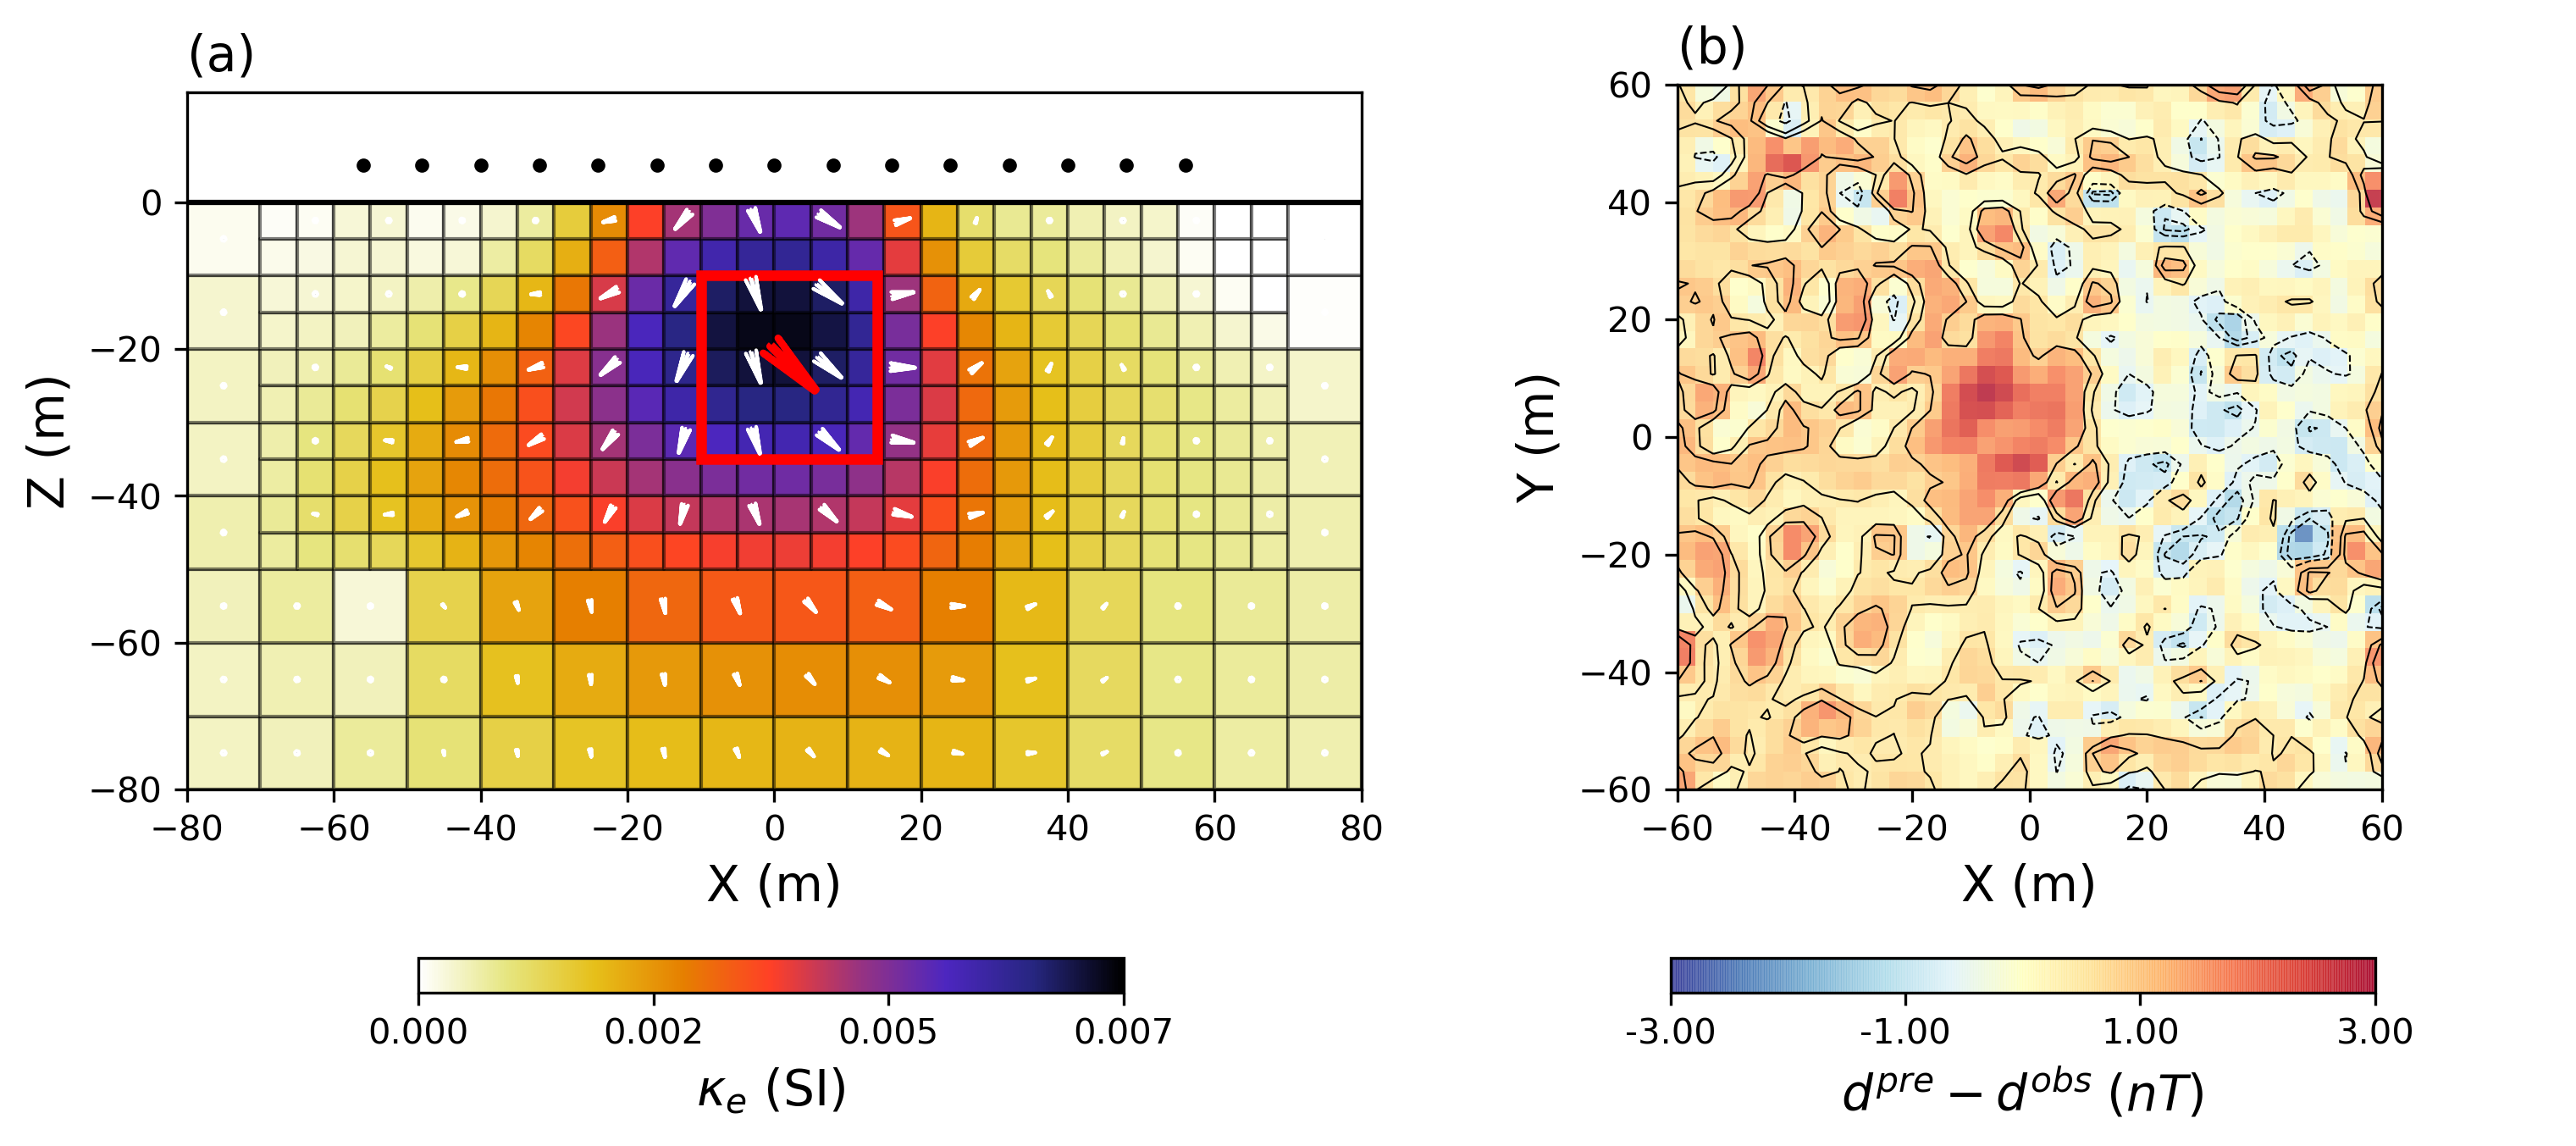
\includegraphics[width=\columnwidth]{Figures/Figure6.png}
\caption{(a) Vertical section through the recovered magnetization vector model in spherical coordinates using sensitivity based weighting and (b) the corresponding data residual map. The same poor starting model shown in Figure~\ref{MVI_S_model_noScale}a was used, but the algorithm converged to a solution similar to the Cartesian solution.}
\label{MVI_S_model}
\end{figure}

From a practical standpoint, we have found that it is more efficient to initialize the MVI-S algorithm with the Cartesian solution. The linear MVI-C approach allows us to rapidly find a model that fits the observed data and it provides a good starting point for the MVI-S formulation. We invert the data once more using the smooth Cartesian solution as a starting model. Figure~\ref{MVI_S_model_lp}a shows the recovered solution obtained after only three iterations of MVI-S. The solution closely resembles the starting Cartesian model. We note, however, that there is some correlated signal in the residual misfit map in Figure~\ref{MVI_S_model_lp}c.

Having achieved a stable and reasonable solution with the $\ell_2$-norm, we can now apply sparse norms to recover a block with a coherent magnetization direction.
We vary the regularization measures on the amplitude, derivatives of amplitude and derivatives of angles uniformly such that ($p_{i_s}$, $p_{i_x}$, $p_{i_y}$ $p_{i_z} = 0$).
Figure~\ref{MVI_S_model_lp}b presents a section through the magnetic vector model. The shape of the anomalous body matches the magnetic block and the magnetization direction is uniform and orientated at $45^\circ$ inclination. Also, the residual data map in Figure~\ref{MVI_S_model_lp}d shows almost no correlated signal. In previous inversions we showed that the data could be fit within the global tolerance $\phi_d \leq \phi_d^*$, but some of the important signal could not be replicated due to the smooth regularization. We have managed to better replicate the fields of a compact source by using the appropriate sparse and blocky assumptions. This result increases our confidence in our ability to accurately recover the magnetization of geological bodies in 3D, as long as the regularization function is adaptable to the geological settings.

\begin{figure}[p!]
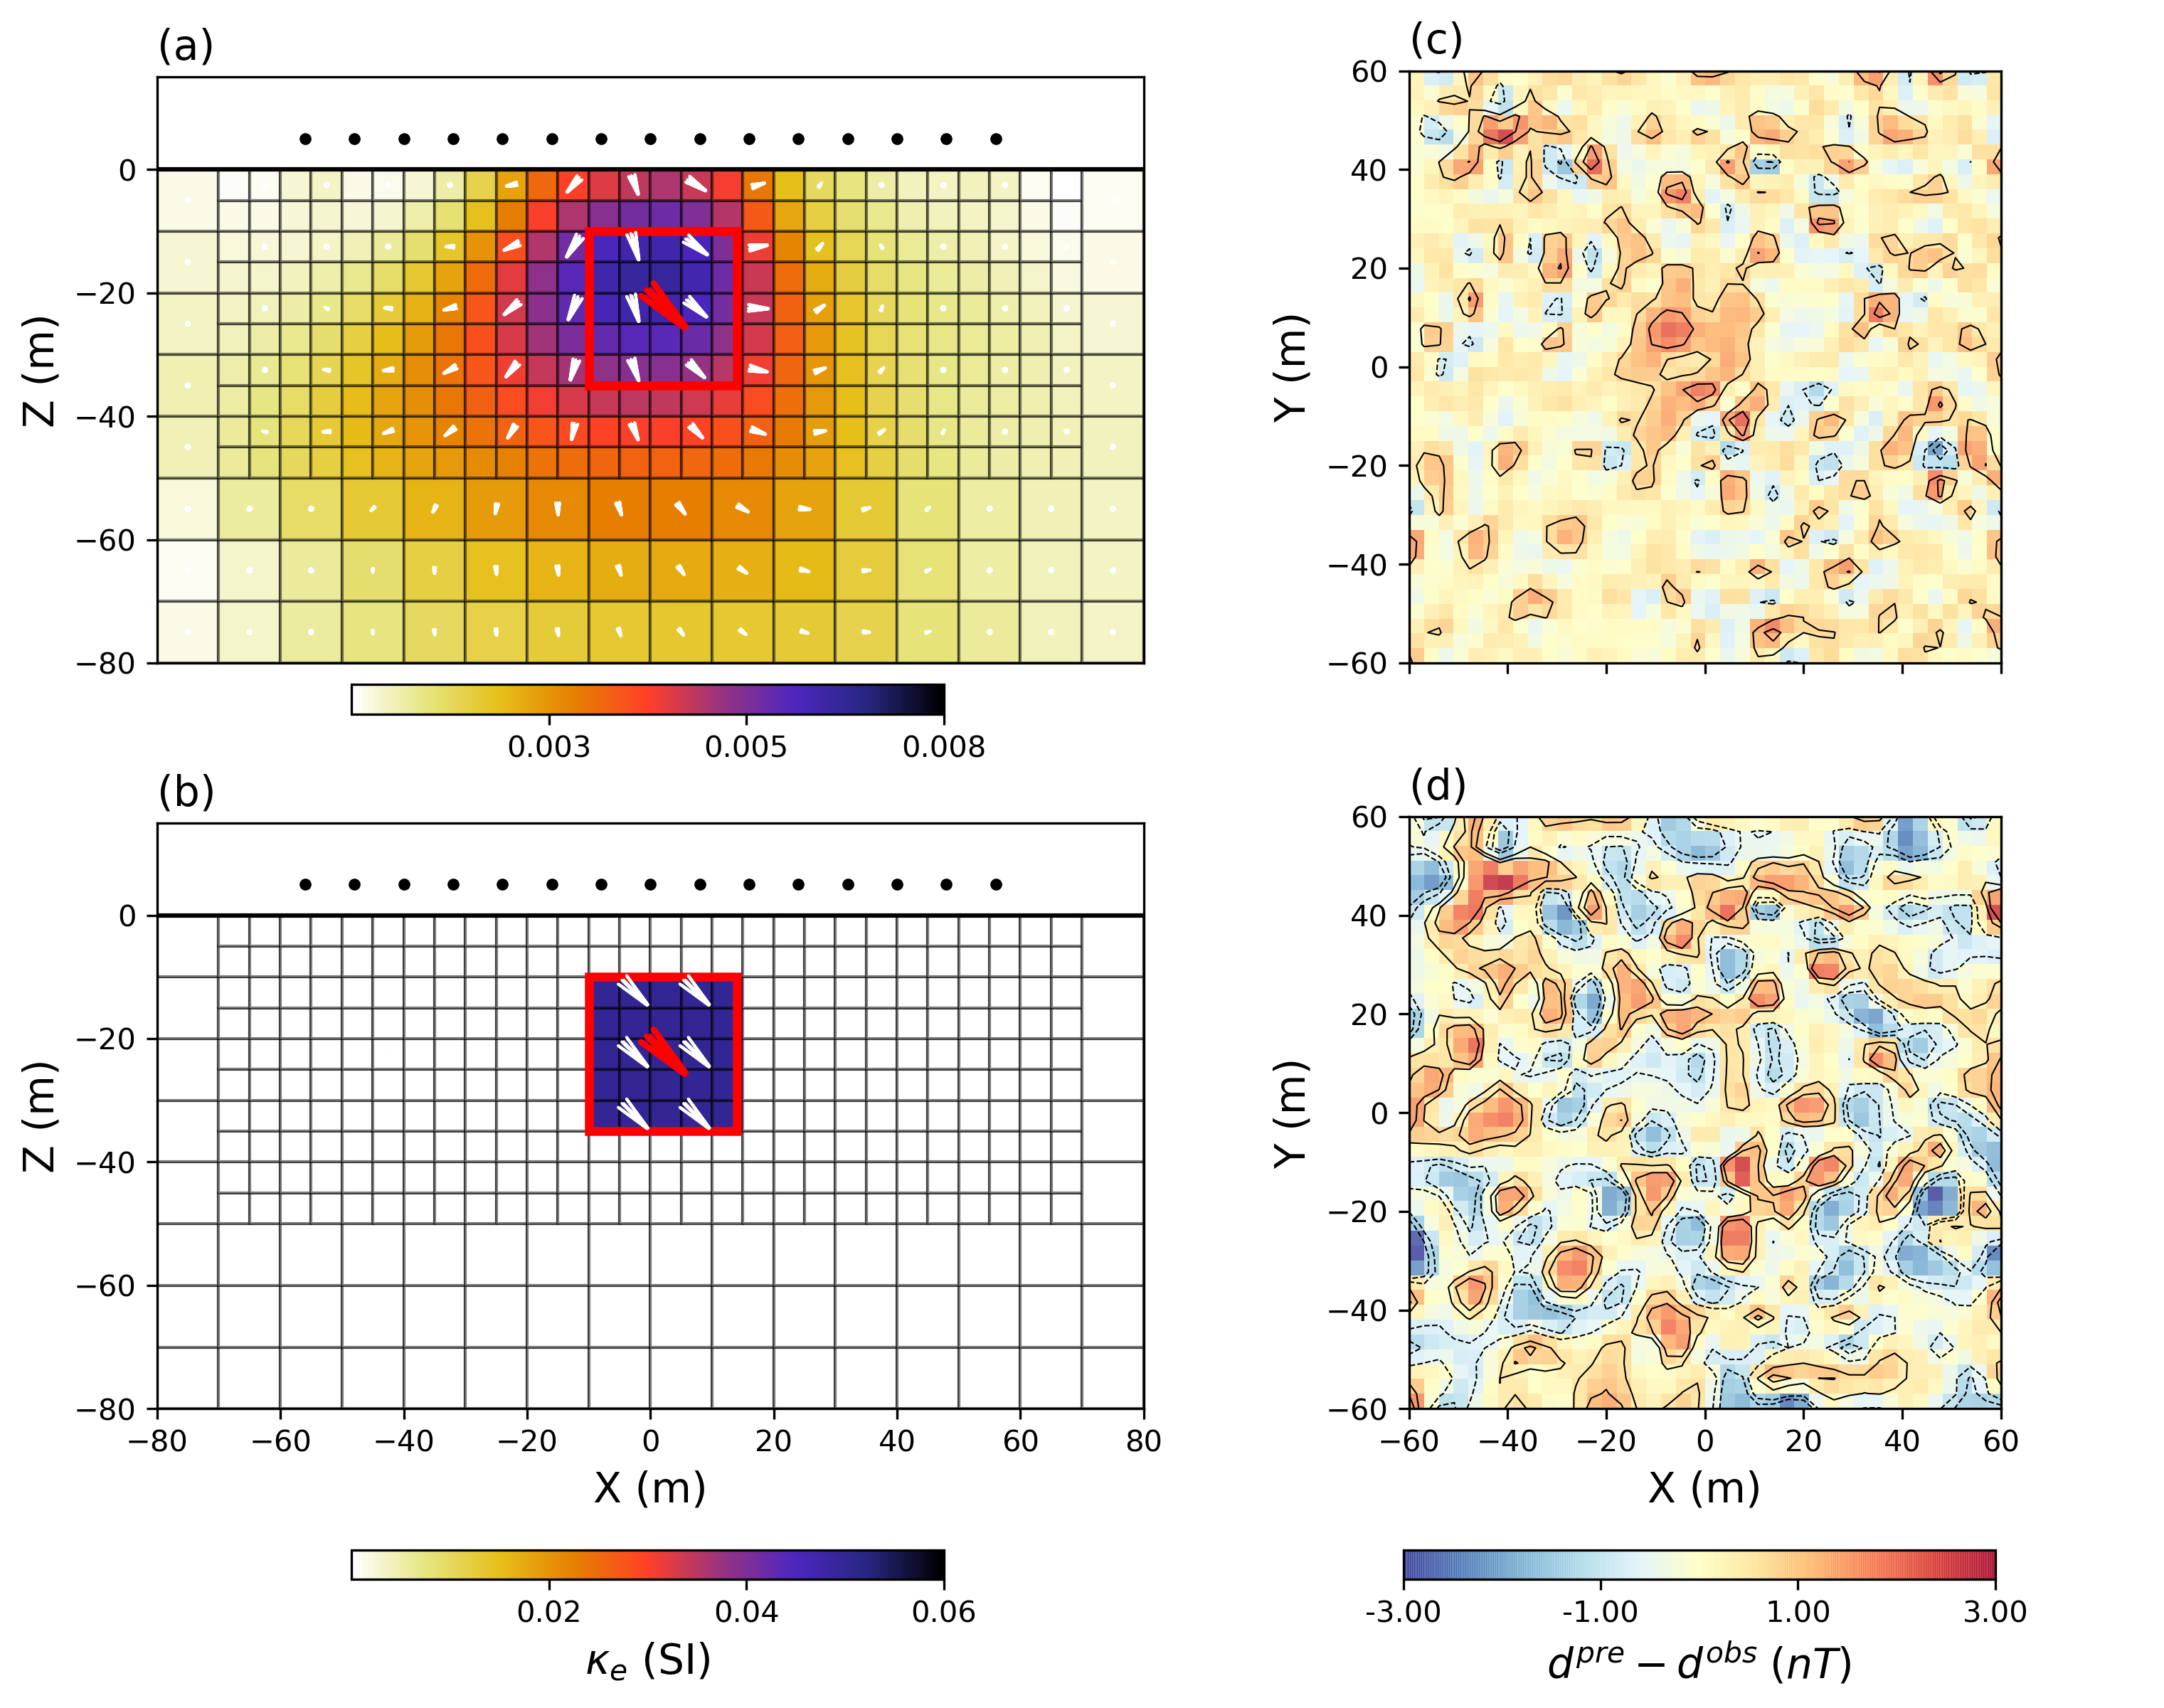
\includegraphics[width=\columnwidth]{Figures/Figure7.png}
\caption{Vertical section through the recovered magnetization vector model in spherical coordinates using sensitivity based weighting and the smooth Cartesian solution as starting model: (a) smooth regularization ($p_s=p_x=p_y=p_z = 2$) and (b) sparse norms on the strength and angles of the magnetization vector ($p_s=p_x=p_y=p_z = 0$). By using the sparse norms, we recover a solution that closely resembles the true model and, as observed in (d), we also eliminate the coherent signal in the residual data that is observed in (c).}
\label{MVI_S_model_lp}
\end{figure}

\section{Case Study: Kevitsa Ni-Cu-PGE deposit}
We demonstrate the capabilities of our inversion strategy with an airborne magnetic survey acquired over the Kevitsa Ni-Cu-PGE deposit, Northern Finland.
The deposit was discovered in the mid-1980s through exploration programs sponsored by the Geological Survey of Finland.
The geology of the deposit has been studied extensively over the past three decades by using  surface mapping and borehole logging.
Figure \ref{Kevitsa_Geology}a presents a simplified geological map of the Kevitsa-Satovaara intrusive complex, adapted from \cite{Koivisto2015}.

\begin{figure}[p!]
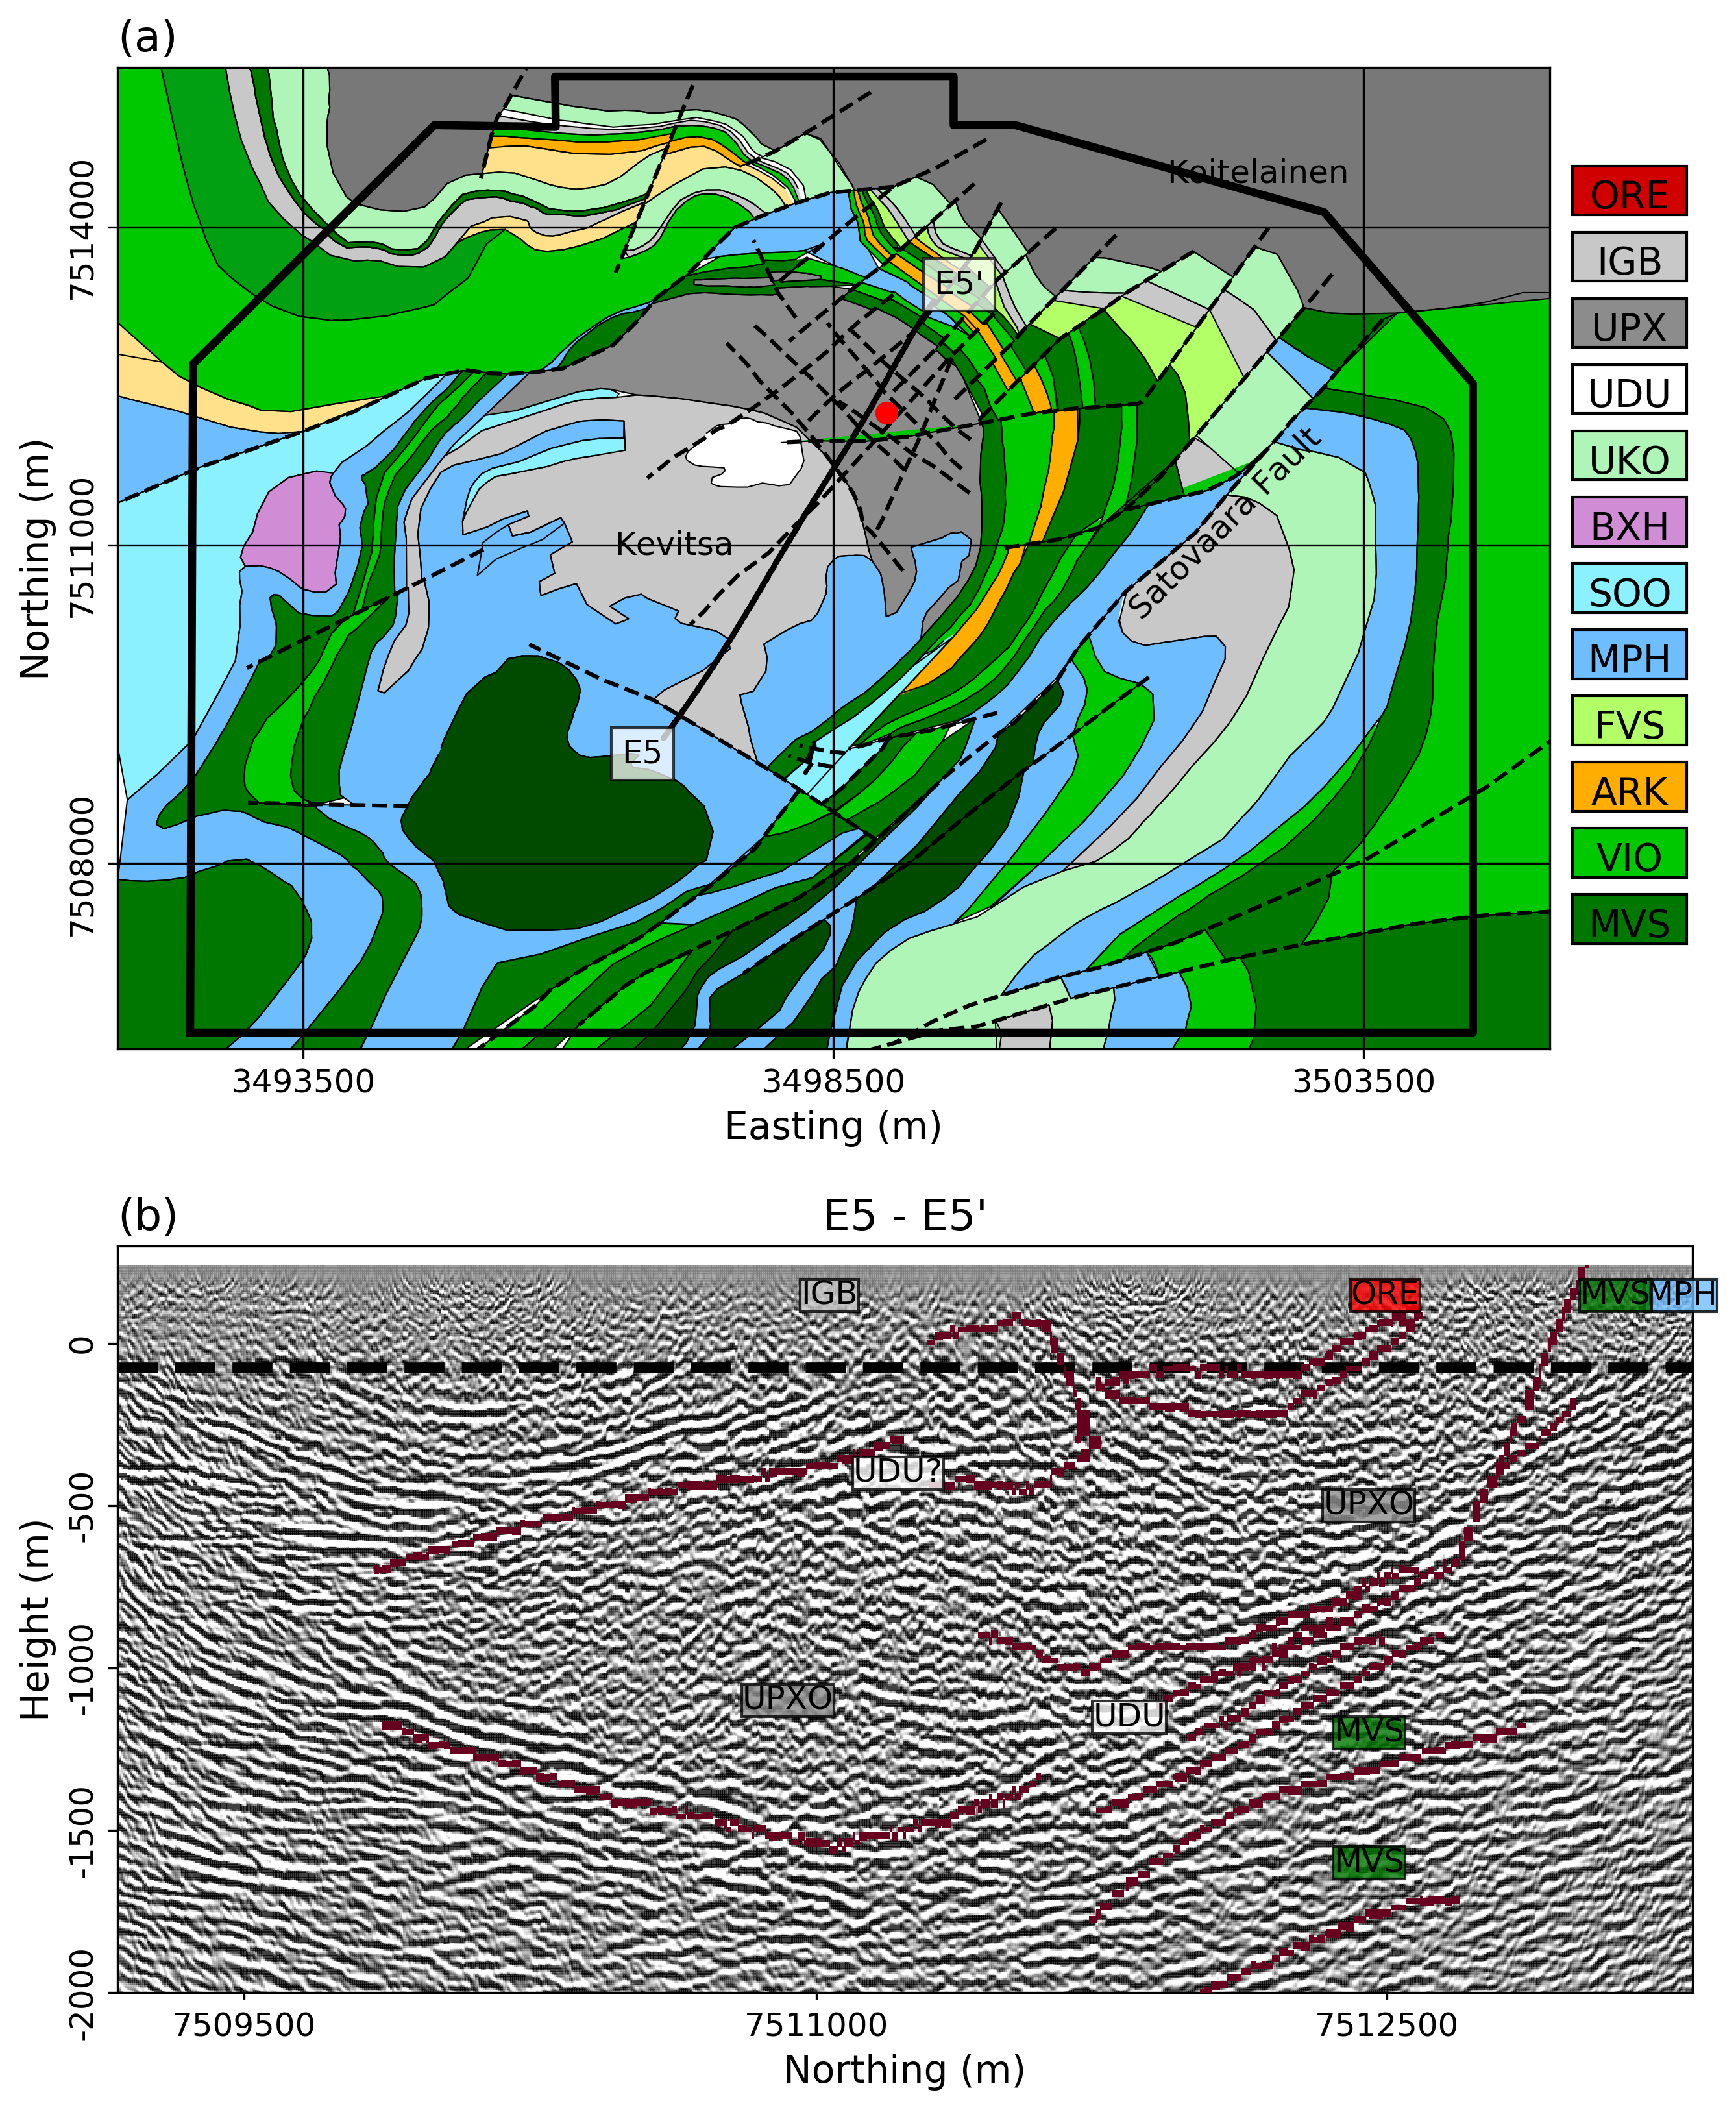
\includegraphics[width=\columnwidth]{Figures/Figure8.png}
\caption{(a) Geological map of the Kevitsa-Satovaara intrusive complex adapted from \cite{Koivisto2015}, with geological definition provided in Table~1. Mapped faults (dash) are shown for reference. (b) 2D seismic line reflection line E5 with interpreted geological contacts between the main reflectors.}
\label{Kevitsa_Geology}
\end{figure}

% \begin{table}
\documentclass[paper]{geophysics}
\usepackage{graphicx}
\usepackage{amsmath}
\usepackage{amsfonts}
\usepackage{multirow}
\usepackage{mathtools}

\usepackage{xcolor}
\newcommand\crule[3][black]{\textcolor{#1}{\rule{#2}{#3}}}
\renewcommand{\arraystretch}{0.5}

\definecolor{BXH}{RGB}{208, 140, 212}
\definecolor{BXHC}{RGB}{218, 150, 222}
\definecolor{UDU}{RGB}{230, 230, 230}
\definecolor{IGB}{RGB}{200, 200, 200}
\definecolor{IGP}{RGB}{128, 0, 128}
\definecolor{IGBM}{RGB}{170, 170, 170}
\definecolor{UPX}{RGB}{140, 140, 140}
\definecolor{UPXO}{RGB}{140, 140, 140}
\definecolor{UKO}{RGB}{176, 245, 184}
\definecolor{VTU}{RGB}{0, 160, 18}
\definecolor{MVO}{RGB}{0, 120, 0}
\definecolor{VBA}{RGB}{0, 90, 0}
\definecolor{VMO}{RGB}{0, 120, 0}
\definecolor{VFO}{RGB}{178, 255, 104}
\definecolor{SAK}{RGB}{255, 174, 0}
\definecolor{SAN}{RGB}{255, 225, 140}
\definecolor{MSC}{RGB}{150, 140, 140}
\definecolor{MPHB}{RGB}{110, 190, 255}
\definecolor{MPH}{RGB}{139, 241, 255}
\definecolor{SOO}{RGB}{139, 241, 255}
\definecolor{VOO}{RGB}{0, 200, 0}
\definecolor{OVB}{RGB}{255, 255, 0}

\begin{document}

\begin{table}
\begin{tabular}{|c | c| l | c |}\hline
& Code & Description & Susceptibility \\ \hline
\crule[OVB]{0.25cm}{0.25cm} & OVB & Overburden & Medium \\ \hline
\crule[IGB]{0.25cm}{0.25cm}& IGB &
\begin{tabular}{l}
IGB: Gabbro \\
IPG: Pegmatite \\
IGBO: Olivine gabbro\\
IDI: Diorite \\
IDB: Diabase \\
IMO: Intrusive (mafic)\\
IGBM: Magnetite gabbro
\end{tabular} & \begin{tabular}{c} \\ Medium \\ \\ \\ \\ \\ \hline High \end{tabular} \\ \hline
\crule[UPX]{0.25cm}{0.25cm}& UPX &
\begin{tabular}{l}
UPXO: Olivine peroxinite \\
UOO: Ultramafic (Undiff.)\\
MPE: Metaperidotite \\
UWB: Websterite \\
\end{tabular} & Medium \\ \hline
\crule[UDU]{0.25cm}{0.25cm}& UDU &
\begin{tabular}{l}
UDU: Dunite \\
UPE: Peridotite \\
\end{tabular} & High \\ \hline
\crule[UKO]{0.25cm}{0.25cm} & UKO & Komatiite & High \\ \hline
\crule[BXH]{0.25cm}{0.25cm} & BXH & \begin{tabular}{l}BXO (undiff.) \\ BXHC: Hydrothermal (crackle)\end{tabular} & Medium \\ \hline
\crule[SOO]{0.25cm}{0.25cm}& SOO &
\begin{tabular}{l}
MAB: Albitite \\
MAM: Amphibolite\\
MQZ: Quartzite \\
MSCSD: Schist \\
\end{tabular} & Low \\ \hline
\crule[MPHB]{0.25cm}{0.25cm}& MPH &
\begin{tabular}{l}
MPH: Phyllite \\
MPHB: Black Phyllite \\
MSCBK: Black Schist \\
MHF: Hornfels \\
\end{tabular} & Low \\ \hline
\crule[VMO]{0.25cm}{0.25cm}& MVS &
\begin{tabular}{l}
VMO: Volcanic Mafic \\
VBA: Basalt\\
VTUM: Volcanic tuff \\
\end{tabular} & Low \\ \hline
\crule[VOO]{0.25cm}{0.25cm}& VIO &
\begin{tabular}{l}
VIO: Volcanic Intermediate \\
VTUI: Volcanic tuff \\
VAN: Andesite \\
VOO: Volcanic (undiff.) \\
\end{tabular} & Medium \\ \hline
\end{tabular}
\end{table}


\end{document}



% \caption{Intervals along boreholes KV200 and KV297 reporting significant remanent magnetization.}
% \label{Table1}
% \end{table}

The Ni-Cu-PGE mineralization is hosted in a funnel shaped ultramafic olivine pyroxenite (UPXO) unit, bordered to the south-west by a gabbro (IGB) unit. The intrusion is hosted in a layered sequence of mafic volcanic (MVS) to intermediate volcanic (VIO) and carbonaceous phyllites (MPH) units. This sequence is interbedded with discontinuous layers of arkose (ARK), arenite (ARN), and felsic volcanic (FVS) units.

It is believed that the disseminated sulphide mineralization within the UPXO unit may have precipitated from the dissolution of Proterozoic Ni-Cu-PGE rich MPH units and sulfur rich evaporates \cite[]{Mutanen1997}. From seismic reflection surveys and borehole data, \cite{Koivisto2015} identified geological contacts at a depth $>1$ km that defines the base of the intrusion (Figure~\ref{Kevitsa_Geology}b).
A large dunite (UDU) block is located in the center of the intrusion. Thick lenses of dunite below the base of the Kevitsa intrusion were identified, as well as a vertical unit between the IGB and UPXO units. While the extent and geometry of these UDU units are not well understood, we expect the dunite be serpentinized and hence highly magnetic.
Table~\ref{Table2} provides a relative ranking of expected magnetization strength based upon the compilation of 105,000 susceptibility readings made on cores from 279 boreholes. Figure~\ref{Kevitsa_PhysProp} summarizes the susceptibility measurements grouped by lithologies.


\documentclass[paper]{geophysics}
\usepackage{graphicx}
\usepackage{amsmath}
\usepackage{amsfonts}
\usepackage{multirow}
\usepackage{mathtools}

\usepackage{xcolor}
\newcommand\crule[3][black]{\textcolor{#1}{\rule{#2}{#3}}}
\renewcommand{\arraystretch}{0.5}

\begin{document}

\begin{table}
\begin{tabular}{|c|c|c|c|c|c|}
\hline
Hole ID & Interval (m) & $\kappa$ (SI) & Inc. ($\circ$) & Q\\
\hline
KV297 & 0-52.9 & $0.034$ & $-42.4$&$[2, 10] $\\
\hline
KV200 & 29.9 & $0.038$ & $-50.9$&$ 5.4$\\
\hline
\end{tabular}
\label{MagCoreSamples}
\end{table}

\end{document}




\begin{figure}[p!]
\includegraphics[width=\columnwidth]{Figures/Figure9.png}
\caption{Whisker plot of magnetic susceptibility measured along 279 boreholes. The coloured boxes have a width scaled by the calculated standard deviation and centered on the mean value for all intercepts belonging to the same lithological classification, as defined in Table~1. The black lines on either side define the minimum and maximum values. The different lithologies are colour coded and grouped based on relative age and similarities in physical properties.}
\label{Kevitsa_PhysProp}
\end{figure}

The deposit is interesting from a geophysical perspective due to the large number of data acquired and made available to researchers: borehole petrophysical measurements, direct-current resistivity, magnetotelluric, ground gravity and magnetic data as well as two airborne time-domain EM surveys (VTEM 2009, SkyTEM 2010).
In this study, we focus our efforts on the magnetic data collected during the 2009 VTEM survey, presented in Figure~\ref{Kevitsa_TMI}. The inducing field parameters at the time of acquisition were $B_0\;[A:\:52,800\: \text{nT}, I:\:77.5^\circ, \;D:\:12.2^\circ]$.

\begin{figure}[p!]
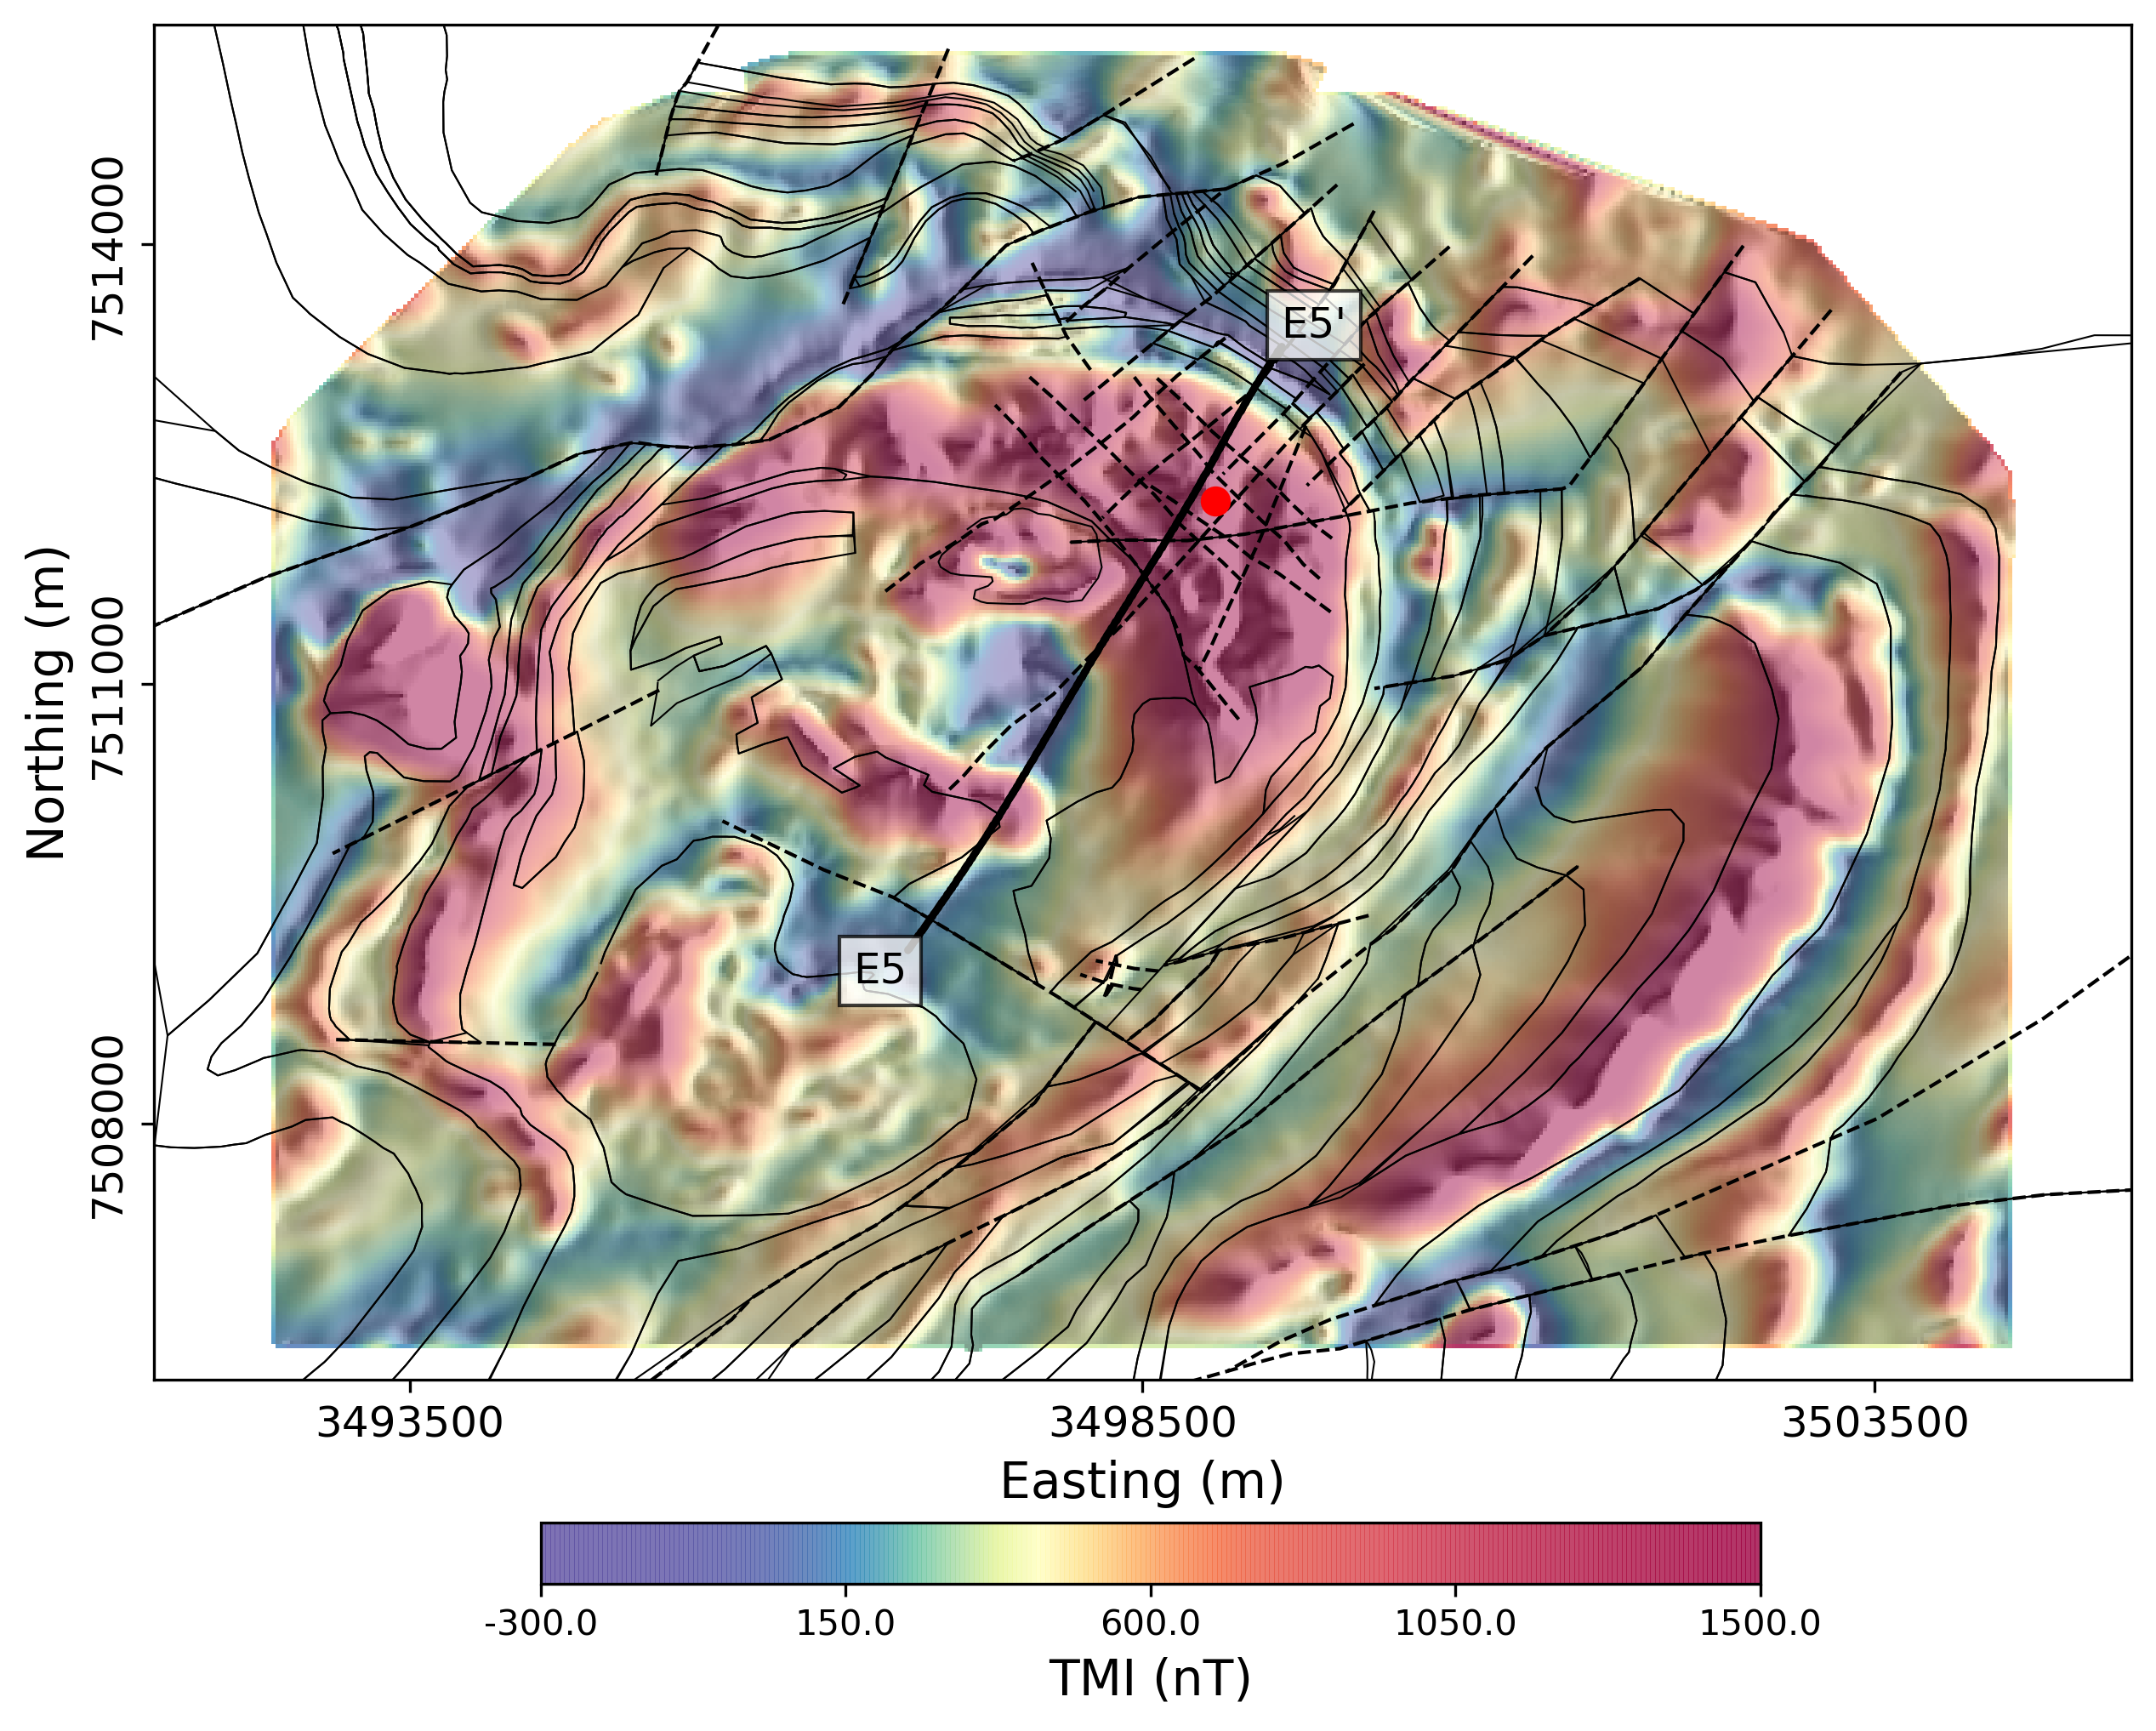
\includegraphics[width=\columnwidth]{Figures/Figure10.png}
\caption{Observed TMI data over the Kevitsa intrusion with histogram equalized color scale. Geological contacts (black), faults (dash) identified from surface mapping and the 2D seismic line locations E5, are shown for reference. Sun shading from east is added to highlight subtle features (Azimuth: $270^\circ$, Dip: $45^\circ$).}
\label{Kevitsa_TMI}
\end{figure}

\begin{table}
\caption{Summary table grouping the various lithological units logged from boreholes. Expected magnetic susceptibility contrasts are derived from Figure~\ref{Kevitsa_PhysProp}.}
\label{Table2}
\end{table}

From visual inspection, we note some obvious connections between the observed TMI data and the surface geology:
\begin{itemize}
\item Strong magnetic signal correlated with the UKO, UPXO and hydrothermal BXH
\item Moderate response from the MVS and VIO
\item Weak fields over most of the MPH units
\item Large negative anomaly within the UDU and near the southern edge of UPXO
\end{itemize}
The strong negative field observed over the dunite unit within the UPXO is of particular interest for this study since it is likely related to remanent magnetization.
Analysis of core samples indicates large Koenigsberger ratios and reversed magnetization direction in the UDU unit as summarized in Table~\ref{Table1} \cite[~p.~47]{Montonen2012}. It is important to note that large Koenigsberger ratios were also measured in the lower UPXO unit, although susceptibility values remained small. In the absence of oriented core, no magnetic declinations were provided. From forward modeling of magnetized sheets, \cite{Montonen2012} estimated that a magnetized unit with effective susceptibility 0.82 SI and orientated $[I=-42.5^\circ, D=240^\circ]$ could be responsible for the observed negative magnetic anomaly.

\subsection{Magnetic susceptibility model}
As a first pass, we invert the TMI data for a smooth susceptibility model ($p_s=p_x=p_y=p_z=2$) and ignore the effects of remanence.
To invert this large dataset we resort to a tiled-Octree mesh decoupling strategy \cite[]{Haber2014}. Sensitivity calculations are performed on nested sub-meshes to reduce the memory footprint required for the forward calculations. The dense sensitivity matrices are stored on disk in \texttt{zarr} file format and accessed in parallel using the open-source \texttt{Dask} library \cite[]{dask2016}. The combination of both the forward mesh decoupling and lazy-loading of sensitivities allows us to run large problems on a desktop computer without the need for compression. The inversion algorithm is written under the open-source SimPEG package in Python \cite[]{Cockett2015}. More details regarding the algorithm are provided in \cite{FournierPhD2019}(p.13). The full inversion domain comprises over 500,000 cells and 17,000 data points.

From sections through the recovered susceptibility model, presented in Figure~\ref{MAG_lp_EW}a and \ref{MAG_lp_EW}b, we note discrepancies with the known geology:
\begin{itemize}
\item In plan view, the arc shaped anomaly, SW of the deposit, is recovered outside the mapped UKO unit.
\item Along the E5 seismic section, no susceptibility anomaly is recovered over the central dunite. This  directly contradicts the core sample measurements made by \cite{Montonen2012}.
\item The shape and extent of the large anomaly correlates poorly with the UPXO unit interpreted by \cite{Koivisto2015} from seismic reflectors.
\end{itemize}
It is also important to note the large correlated residuals shown in Figure~\ref{MAG_lp_EW}c. The inversion had difficulty finding a strictly positive susceptibility model that could account for both the large positive and negative fields. This is a good indicator that the magnetic response observed at Kevitsa cannot solely be attributed to an induced magnetization alone.

\begin{figure}[p!]
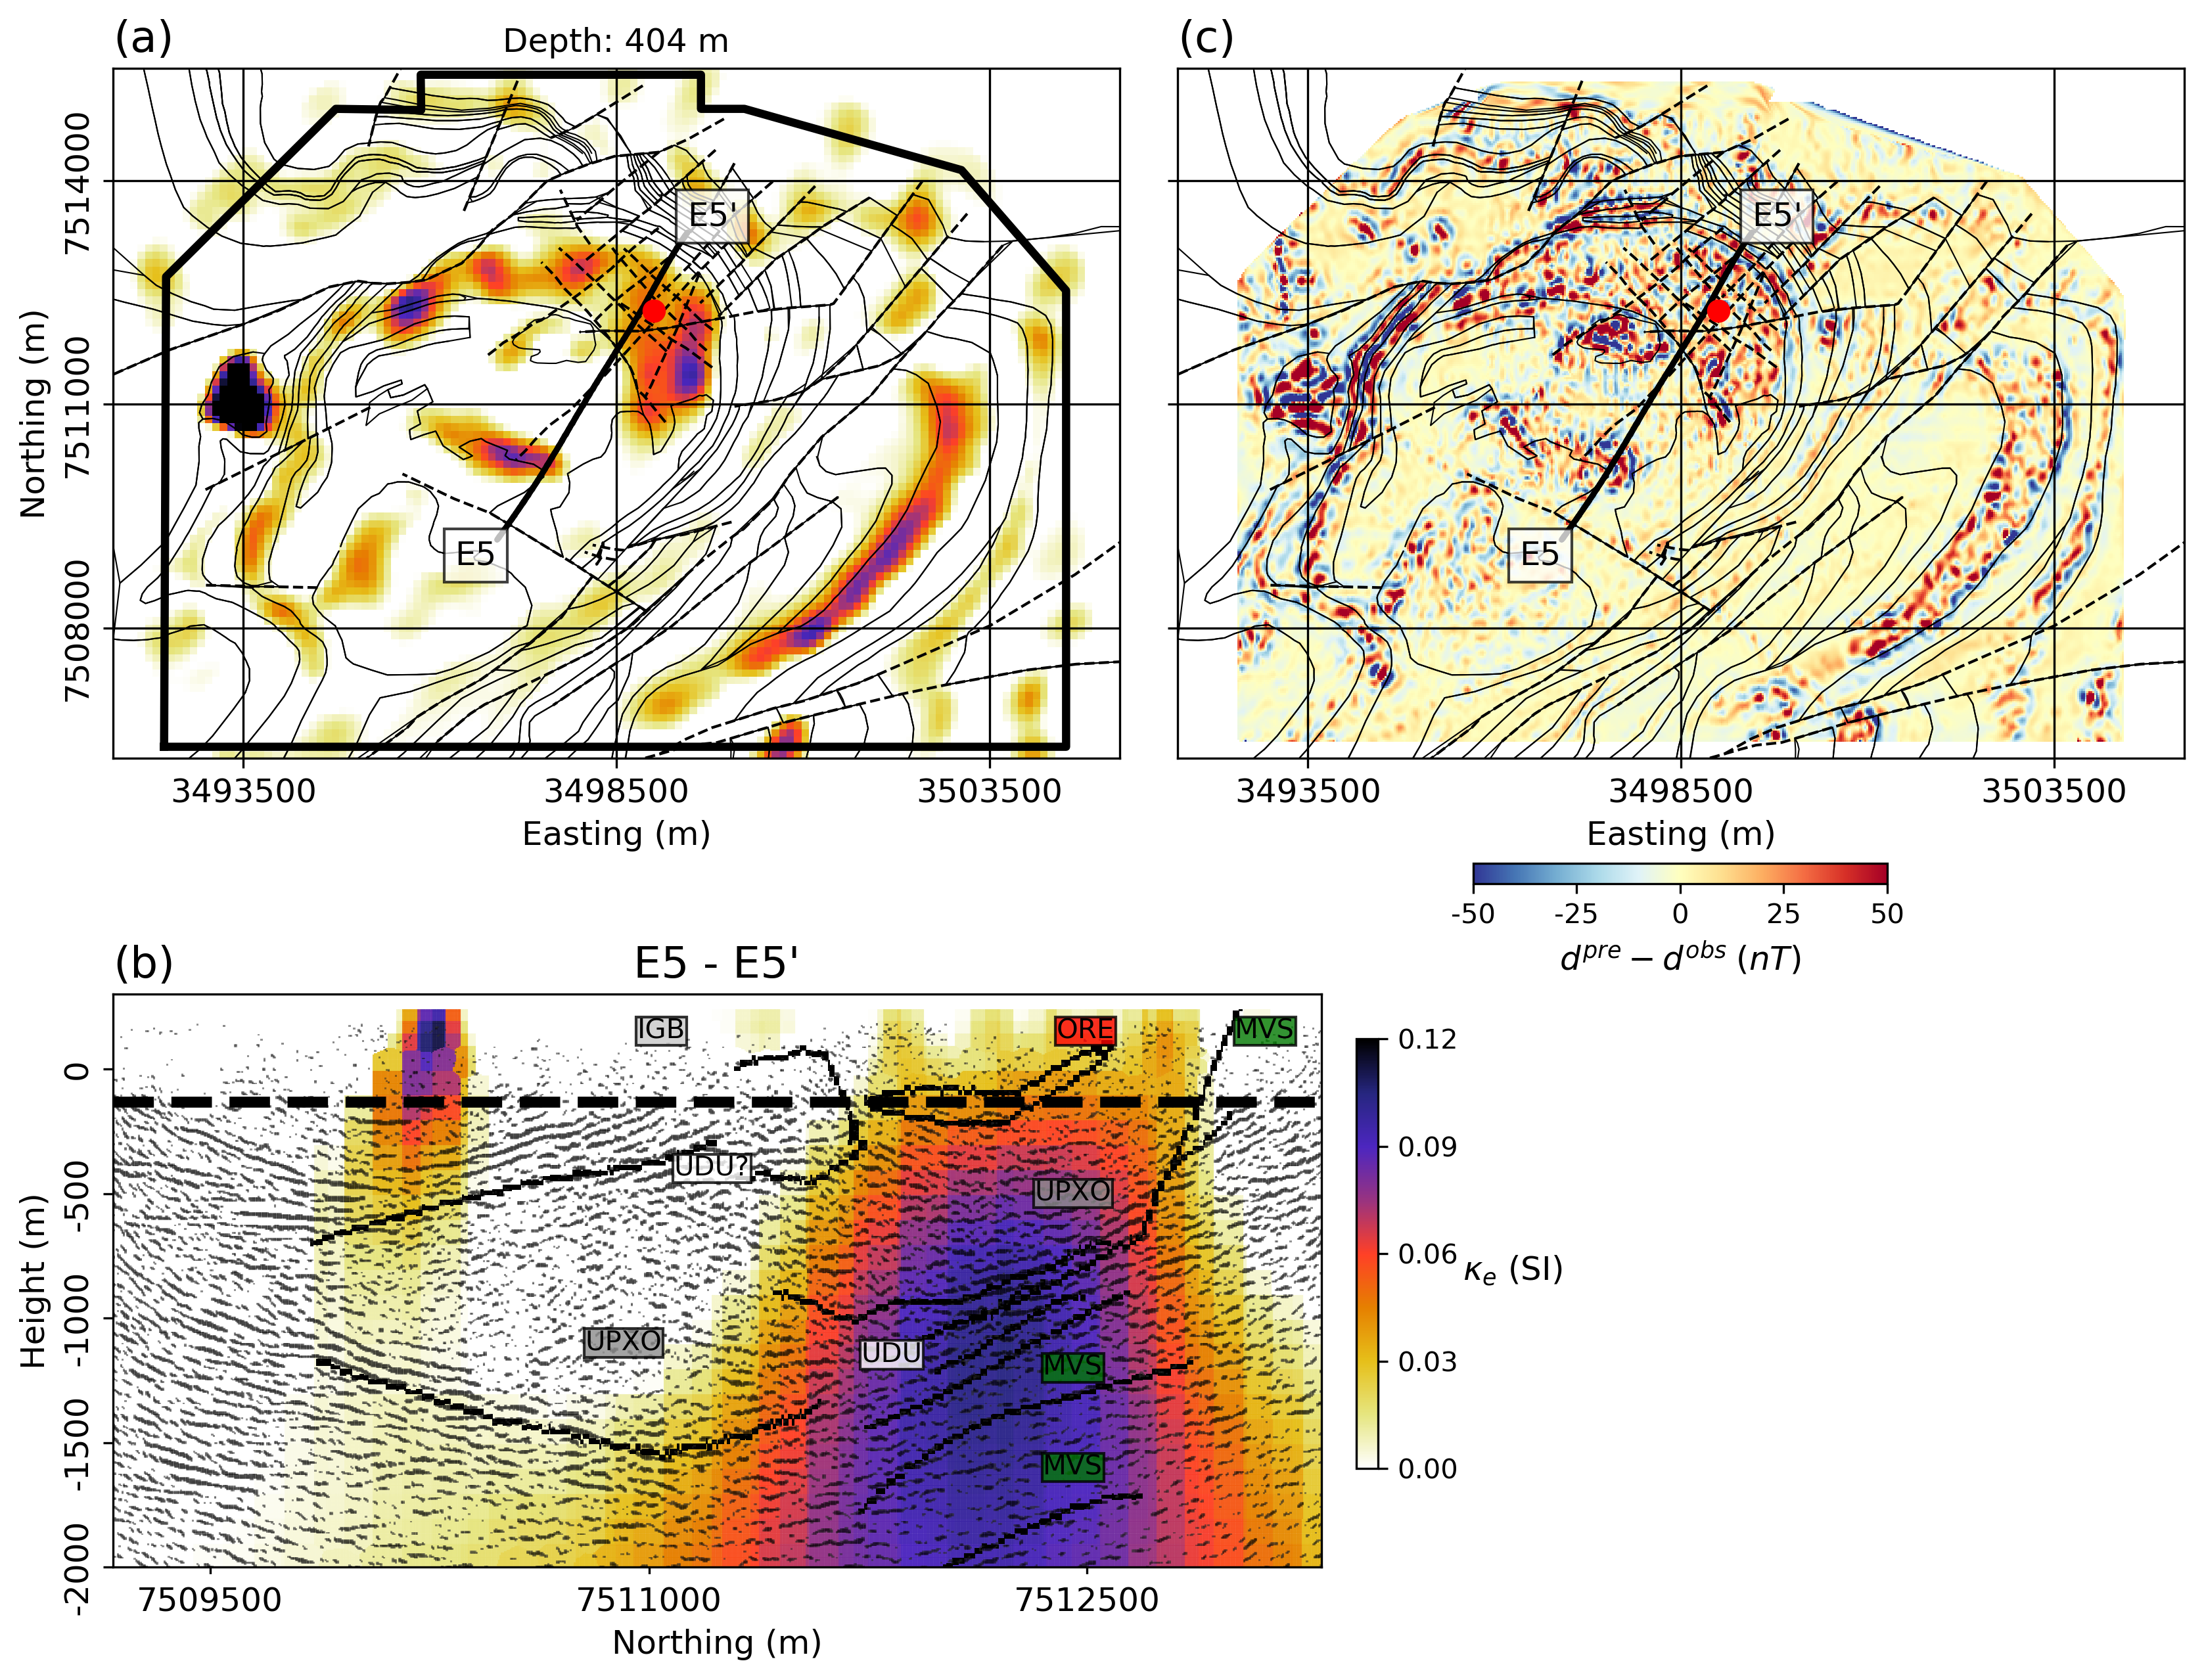
\includegraphics[width=\columnwidth]{Figures/Figure11.png}
\caption{(a) Horizontal and (b) vertical sections through the recovered susceptibility model that ignores the effect of remanence. Lithological contacts (black) identified by \cite{Koivisto2015} are shown for reference. (c) The residual map shows strong correlation with the negative magnetic data.}
\label{MAG_lp_EW}
\end{figure}

\subsection{Magnetization vector model}
To address the issues posed by remanence, we proceed with the MVI-S algorithm.
We perform a series of nine inversions with varying sparsity measures to assess the variability in the magnetization model. Starting from a common $\ell_2$-norm MVI-C model, we sequentially vary the combination of norms applied to the amplitude and its derivatives for ($p_{\rho_s}, p_{\rho_{xyz}} \in [0, 2]$). In all cases, we fix the $\ell_p$-norm regularization on the derivatives of the angles ($p_{\theta_{xyz}},\;p_{\phi_{xyz}} =0$) to promote coherent magnetization orientations.

Horizontal and vertical sections through the recovered nine magnetization models are shown in Figures~\ref{MVIS_Hsections} and \ref{MVIS_Vsections}, respectively.

\begin{figure}[p!]
\includegraphics[width=\columnwidth]{Figures/Figure12.png}
\caption{Horizontal sections at $\approx$ 300 m below topography for a suite of models using various sparsity assumptions put on the amplitude of magnetization for $p_s\;, p_{x,y,z} \in [0,\: 2]$. Norm measure on the magnetization angle are fixed to $p_{x,y,z}=0$ in order to promote uniform magnetization direction.}
\label{MVIS_Hsections}
\end{figure}

\begin{figure}[p!]
\includegraphics[width=\columnwidth]{Figures/Figure13.png}
\caption{Vertical sections along the E5 seismic reflection line for a suite of models using various sparsity assumptions put on the amplitude of magnetization for $p_s\;, p_{x,y,z} \in [0,\: 2]$. Norm measure on the magnetization angle are fixed to $p_{x,y,z}=0$ in order to promote uniform magnetization direction.}
\label{MVIS_Vsections}
\end{figure}

To simplify the analysis, we superimpose the $90^{th}$ percentile iso-value of amplitude for each of the nine models (Figure~\ref{MVIS_Vsections}). We calculate an average magnetization direction (white) and standard deviation on the angle (red). We observe the following:

\begin{itemize}
\item Parts of the central dunite (UDU) unit appear to be reversely magnetized $[\kappa_{e} = 0.09\;SI, \;I=-52^\circ \pm 15^\circ, \;D=246^\circ \pm 5^\circ]$. The recovered inclination in the model cells nearest to the published results from \cite{Montonen2012} agree well.
\item A tabular magnetic anomaly between the IGB and UPX unit, likely related to the central dunite unit, appears to be plunging towards SE, potentially extending below the UPX unit as hypothesized by \cite{Koivisto2015}.
\item Strong magnetization recovered along the outershell of the UPX ultramafic intrusion appears to be pointing normal to its base.
\item Similar radial outward magnetization recovered along the arc-shaped UKO unit, east of the Kevitsa deposit.
\end{itemize}
The last two remarks are interesting for a few reasons. First, strong magnetization near the base of the ultramafic supports the presence of magnetic UDU units below the intrusion.
Second, the orientation of magnetization pointing radially outward may be indicative of past tectonic deformation.
Under the assumption that the remanent magnetization component had been fairly uniform within the layered UDU, UKO and UPX unit at the time of formation, then the current radiating magnetization pattern would be explained by subsequent folding of the units.
If this is the case, than it would be one of the most complex geological scenarios for which magnetic data inversions have been used to infer tectonic deformation.

While our modeling of the central dunite unit agrees with published laboratory measurements, the cause for this reverse magnetization direction remains unclear. No other lithological units appear to share this orientation. Re-magnetization after emplacement of the ultramafic intrusion is unlikely as a similar reversed polarity pattern would also be expected elsewhere at Kevitsa. We speculate that the dunite block could be related to the lower UDU unit, which would have been folded to its current sub-vertical location.


\section{Conclusion}
In this study, we introduced an iterative sensitivity re-weighting strategy to improve the convergence of the non-linear MVI-S formulation.
The iterative re-scaling of the regularization function associated with the amplitude and angles of magnetization was crucial in order to achieve stable convergence of the algorithm.
Smoother and more robust solutions allowed us to apply compact norms on the three model parameters independently, which greatly simplified the solution over the conventional MVI-C formulation. Despite this improvement, the MVI problem remains largely under-determined. Incorporating $a \; priori$ information, either through model constraints or joint physical properties, remains important to accurately represent the geology.

We demonstrated the capability of the newly accessible MVI-S formulation on an airborne magnetic survey collected over the Kevitsa Ni-Cu-PGE deposit. The recovered effective susceptibility and magnetization model confirmed that the central dunite unit was associated with strong reversed magnetization oriented roughly [$\kappa_{e} = 0.09$ SI, $I=-52^\circ \pm 15^\circ$, $D=246^\circ \pm 5^\circ$].
Potentially the most significant outcome of this case study is the recovered sparse magnetization pointing normal to the base of the Kevitsa olivine-pyroxenite unit. If confirmed by laboratory measurements, this result would be one of the few paleomagnetic interpretations carried over folded geology that is based on the inversion of airborne magnetic data.

\section{Acknowledgments}
The authors would like to thank Markku Montonen at New Boliden for given us access to the geophysical data. Special thanks to Dr. Emilia Koivisto at the University of Helsinki for providing the 3D geological surfaces and interpretation and Dr. Frank Santaguida for providing the background information and putting us in contact with key people. Last but not least, we are grateful to the open-source community, in particular, those that contributed to the \texttt{Dask} and \texttt{SimPEG} packages.

\pagebreak
% \documentclass[paper]{geophysics}
\usepackage{graphicx}
\usepackage{amsmath}
\usepackage{amsfonts}
\usepackage{multirow}
\usepackage{mathtools}

\usepackage{xcolor}
\usepackage{setspace}

\newcommand\crule[3][black]{\textcolor{#1}{\rule{#2}{#3}}}
\renewcommand{\arraystretch}{0.5}
\doublespacing
% --- Defining math operators ---
\newcommand{\curl}[1]{\ensuremath{\nabla\times \mathbf{#1}}}
\newcommand{\curlSym}[1]{\ensuremath{\nabla\times \boldsymbol{#1}}}
\renewcommand{\div}{\nabla\cdot\,}
\newcommand{\mb}[1]{\ensuremath { {\mathbf #1}}}
\newcommand{\mbSym}[1]{\ensuremath{\boldsymbol{#1}}}
\renewcommand{\deg}{\ensuremath{^\circ}}
\pdfoptionpdfminorversion=6

\graphicspath{{./High-Res/}}

% -----------
\begin{document}

% --- Geophysics: ---
\title{Sparse magnetic vector inversion in spherical coordinates}

\begin{center}
{\LARGE\textbf{Sparse magnetic vector inversion in spherical coordinates}}
%\maketitle{}

\author{Dominique Fournier\footnotemark[1], Lindsey J. Heagy\footnotemark[2] and Douglas W. Oldenburg\footnotemark[1]}
{Dominique Fournier$^1$, Lindsey J. Heagy$^2$ and Douglas W. Oldenburg$^1$

\vspace{10 mm}
Right Running Head: Sparse magnetic vector inversion
\vspace{10 mm}


$^1$ Geophysical Inversion Facility, Department of Earth, Ocean, and Atmospheric Sciences,
University of British Columbia, Canada. E-mail: dfournie@eoas.ubc.ca, doug@eoas.ubc.ca

$^2$ Department of Statistics, the University of California, Berkeley, California. E-mail: lheady@berkeley.edu
}
\end{center}

\righthead{Sparse magnetic vector inversion}


\begin{abstract}
Magnetic vector inversion has received considerable attention over recent years for processing magnetic field data that are affected by remanent magnetization. However, the magnetization models obtained with current inversion algorithms are generally too smooth to be easily interpreted geologically. To address this, we review the magnetic vector inversion formulated in a spherical coordinate system. We tackle convergence issues posed by the non-linear transformation from Cartesian to spherical coordinates by using an iterative sensitivity weighting approach and a scaling of the spherical parameters. The spherical formulation allows us to impose sparsity assumptions on the magnitude and direction of magnetization independently and, as a result, the inversion recovers simpler and more coherent magnetization orientations. The numerical implementation of our algorithm on large-scale problems is facilitated by discretizing the forward problem using tiled Octree meshes. All of our results are generated using the open-source SimPEG software. We demonstrate the enhanced capabilities of our algorithm on a large airborne magnetic survey collected over the Kevitsa Ni-Cu-PGE deposit. The recovered magnetization direction inside the intrusive and in the host stratigraphy is consistent with laboratory measurements and provides evidence for tectonic deformation.
\end{abstract}


\section{Introduction}
The study of magnetism in rocks has a long history in Earth sciences and continues to play a key role in mineral exploration and tectonic studies \cite[]{NATOASIS1989, Pueyo2016, Li2019}. Magnetic susceptibility, the ability of rocks to become magnetized by the geomagnetic field, is a useful property for mapping geology under cover. To this end, a large number of datasets, from global satellite measurements to deposit scale surveys, have been made available over the years. These  data sets  have also brought to light the prevalence of remanent magnetization: a permanent magnetization direction acquired by certain minerals and often associated with mineral deposits such as diamondiferous kimberlites, volcanogenic massive sulphides and porphyry deposits \cite[]{Henkel1991, Enkin2014}. The remanent component of magnetization is typically ignored in the interpretation of magnetic data, and therefore it is often considered as ``noise'' which complicates the geologic interpretation.

Meanwhile, the same remanent component has been used extensively for paleomagnetic studies and regarded as meaningful geophysical “data”. A number of researchers have used the permanent magnetization orientation to map continental block rotation \cite[]{Norris1961, Vine1963, NATOASIS1989}, for fold and thrust belts reconstruction \cite[]{Ramon2012, Villalain2015} and in geochronology \cite[]{Henkel1991, Lockhart2004, Enkin2003}.
While these studies provide valuable information about Earth's history, they have relied primarily on laboratory measurements performed on oriented cores. Analysis based on point measurements of magnetization direction remains a limiting factor in understanding the spatial and temporal variability of large fold and thrust belts systems \cite[]{Pueyo2016}.

Geophysical inversions provide an approach for extracting information about magnetization and constructing a 3D model of the subsurface from observed total magnetic field (TMI) data.
Imaging the shape and depth of magnetic bodies can help identify mineral deposits, while recovering the orientation of magnetization can benefit paleomagnetic studies.
As noted in the review by \cite{Li2017}, inversion strategies for magnetic data put forward in the literature can be broadly grouped into three main categories. In the first group, the magnetization orientation of compact bodies is estimated through search algorithms \cite[]{Fedi1994, DannemillerLi06}, magnetic moment analysis \cite[]{Helbig1963, Phillips03}, and inversion methods. The most common inversion approach uses simple parametric shapes to approximate elongated and tabular bodies \cite[]{Foss2011a, Fullagar2013, Clark2014, Pratt2014}. These methods are computationally inexpensive and work well when the magnetic response can be isolated, but, in practice, they rely heavily on experts to build and test different scenarios; this can become impractical in complex geological settings.

The second group deals with remanence by transforming the field data into a quantity that is weakly sensitive to the orientation of magnetization. Magnetic amplitude data, for example, can be inverted for an effective susceptibility model; this approach was first introduced by \cite[~p.~52]{Shearer05}. While the amplitude inversion method has proven to be successful in identifying geological features \cite[]{Krahenbuhl2007, LiShearer10}, several drawbacks persist. First, the amplitude data must be calculated by pre-processing the observed TMI data either through a Fourier transform or by the equivalent source method \cite[]{LiNabighian14}. This process may introduce unintended biases or numerical errors into the inversion. Secondly, the solution does not provide information about the direction of magnetization unless estimated in post-processing. Thirdly, the conversion to amplitude removes phase information from the data. This makes dip interpretation more difficult.

The third category, which is the focus of this study, aims to recover a 3D distribution of magnetization vectors directly from TMI data. \cite{LelievreOldenburg2009} introduced a Magnetic Vector Inversion algorithm, implemented in both Cartesian (MVI-C) and spherical (MVI-S) coordinate systems.
The MVI-C formulation is closely related to the method proposed by \cite{Kubota2005}, and later adopted by \cite{Ellis2012}. This has substantially improved the interpretation of magnetic data and it is now frequently used by industry.
Solving for a vector model remains difficult however, since it results in a large underdetermined inverse problem with three times the number of variables (i.e. spatial components) compared to conventional inversions. The method relies heavily on the regularization function and often yields a smooth model that is too blurred for direct geological interpretation.
In order to deal with this deficiency, \cite{Li2016} introduce a fuzzy c-means clustering technique to force the magnetization to be in a set number of domains.
Sparsity constraints on the vector components have been proposed, either directly applied to the Cartesian components through Gramian constraints \cite[]{Zhu2015}, or indirectly through a cooperative approach \cite[~p.~101]{Liu2015, Fournier2015}. These `focusing' methods have shown success in better recovering the shape of compact bodies, but ambiguity remains about the magnetization direction.

\cite{LelievreOldenburg2009} advocate the use of the spherical representation so that constraints can be applied independently on the amplitude and orientation angles. This formulation is well-suited for incorporating sparsity and physical property constraints, but its implementation remains challenging. The nonlinear transformation makes the inversion prone to converge to a local minimum. The main reason is that the inversion parameters have different units (length, radian) and their respective sensitivities vary over several orders of magnitude. This issue has partially been addressed in \cite{Liu2017} with a fixed scaling parameter.

In this study, we propose to address the current limitations encountered with the MVI-S algorithm. Building upon the work of \cite{Liu2017}, we define two scaling mechanisms: the first addresses the differing magnitudes of parameters in spherical coordinates and the second compensates for rapid changes in the sensitivity due to the non-linearity of the problem. We demonstrate the benefit of our iterative sensitivity re-weighting strategy on a simple two-parameter problem. Employing a stable MVI-S algorithm allows us to impose penalties on the magnetization direction and amplitude independently, which allows us to recover compact bodies with coherent magnetization direction. We use a tiled Octree mesh decoupling approach to deal with the large memory footprint of the problem; this removes the need for compression. We first showcase our approach on a synthetic block model. The same algorithm is applied to an airborne magnetic field data set acquired over the Kevitsa Ni-Cu-PGE deposit, Finland. We unravel the complex magnetic signal to recover geologic units and their magnetization directions and we recover regions of high magnetization at depth which are in good agreement with known dunite units. The orientation of magnetization is consistent with  previously published measurements performed on core samples. We infer tectonic deformation from the orientation of magnetization recovered within the folded host stratigraphy.

\section{Methodology}
Our goal is to image the subsurface using magnetic field data.
From Gauss's law, the forward relation between magnetization and the magnetic field response can be expressed as:
\begin{equation} \label{b_integral}
\vec{b}(r) = \frac{\mu_0}{4\pi} \int_{V} \nabla \nabla \frac{1}{ r} \cdot \vec{M} \; dV\;,
\end{equation}
where $\vec{b}$ is the magnetic flux density in teslas (T) and $r$ is the radial distance between an arbitrary position and the magnetic source with magnetization per unit volume $\vec{M}$ (A/m).
For most geophysical applications, we do not measure the vector field $\vec b$ of magnetized bodies, but rather the amplitude of the field, or TMI data, that includes both the geomagnetic and secondary fields
\begin{equation}
b^{TMI} = \|\vec b_0 + \vec b \|
\end{equation}
where $\vec b_0 = \mu_0\vec h_0$ is the geomagnetic flux density.
The anomalous field data, $d^{TMA}$, is computed by subtracting $\|\vec b_0\|$ from the TMI data. Thus
\begin{equation}
\begin{split}
{d}^{TMA} &=  \|\vec b_0 + \vec b \| - \|\vec b_0\| \\
&\approx \vec{b}\cdot \hat b_0
\end{split}
\end{equation}
This approximation is valid so long as $\|\vec b\| \ll \|\vec b_0\|$.
In matter, the total magnetization per unit volume can be separated into its induced and remanent components such that:
\begin{equation}\label{Magnetization}
	\vec{M} = \kappa (\vec{h}_0 + \vec{h}_s) + \vec{M}_{r}\;,
\end{equation}
where the magnetic susceptibility $\kappa$ (SI) is the physical property describing the ability of a rock to get magnetized under an applied field. In nature this inducing field has two components: the Earth's geomagnetic field $\vec{h}_0$ and secondary fields $\vec{h}_s$ related to local magnetic anomalies.
The remanent magnetization $\vec{M}_{r}$ is a permanent magnetization preserved in the absence of an inducing field. This is the quantity of interest in the field of paleomagnetism as it preserves information about the inducing field direction and position of a rock at the time of remanence acquisition.

Our goal is to recover a 3D model $m$ describing some quantity related to magnetization ($m:=\vec{M}$) from the observed data.
The inverse problem can be formulated as an optimization problem of the form:
\begin{equation}
\begin{split}\label{GenMinProb}
\underset{{m}}{\text{min}}\; \phi({m}) & = \; \phi_d + \beta \phi_m \\
\text{subject to} \; \phi_d & \leq \phi_d^* \; .
\end{split}
\end{equation}
\cite[~p.~7]{TikhonovArsenin77}.
The objective function $\phi({m})$ has two terms.
The misfit function,
\begin{equation}\label{eq:misfit}
\phi_d =\sum_{i=1}^{N}\left(\frac{{d}_i^{pre} - {d}_i^{obs}}{\sigma_i}\right)^2 \;,
\end{equation}
measures the residual between the predicted data ${d}^{pre} = F[m]$ and observed ${d}^{obs}$ data normalized by estimated uncertainties ${\sigma}$. Assuming that the noise and error on the data are random, our expected target misfit $\phi_d^*=N$, where $N$ is the number of data.
The model objective function, $\phi_m$, also known as the regularization function, is typically made up of several functions that control the magnitude and roughness of the model. The trade-off parameter $\beta$ controls the relative importance between the two competing objectives.
In this research, we use the general $l_p$-norm measure of the model and its spatial gradients as our model objective function
\begin{equation}
\begin{split}\label{intReg}
\phi_m &= \sum_{r=s,x,y,z} \alpha_j \int_V w_r \;|f_r (m)|^{p_r} \;dV\;. \\
\end{split}
\end{equation}
The regularization functions $f_r$ are user-defined but most often have the following form
\begin{equation}
\begin{split}\label{fj}
f_s= m,\;f_x= \frac{d m}{dx},\; f_y= \frac{d m}{dy},\;f_z= \frac{d m}{dz}\;.
\end{split}
\end{equation}
Thus $f_s(m)$ measures the size of $m$ and $f_x(m)$, $f_y(m)$ and $f_z(m)$ measure the roughness along orthogonal directions. These functionals can also include a reference model $m_{ref}$ but for the sake of notation we set it to zero.
Weighting terms $w_r$ allow the user to adjust the strength of the regularization function in specific regions of the inversion domain.

The general strategy to minimize equation 5 requires that we discretize the model onto a mesh (we use $\mathbf{m}$ to denote the discretized model which has length $M$) and find a  solution such that the gradient of the objective function
\begin{equation}\label{gradPhi}
\mathbf{g} = \nabla_m \phi(\mathbf{m}) = \nabla_m \phi_d + \beta \bigg[ \alpha_s \nabla_m \phi_s + \alpha_x \nabla_m \phi_x + \alpha_y \nabla_m \phi_y + \alpha_z \nabla_m \phi_z \bigg] = \mathbf{0} \;.
\end{equation}
A solution to the optimization (equation 5) is found for decreasing values of the trade-off parameter $\beta$; we stop when we find a suitable model that reproduces the data to within a predefined tolerance:
\begin{equation}\label{phidTol}
\frac{|\phi_d- \phi_d^*|}{\phi_d^*} \leq \eta_{\phi_d}\;.
\end{equation}
Building upon the work presented in \cite{FournierDWO2019}, we solve the nonlinear problem in equation 7 by the Scaled Iteratively Reweighted Least Squares (S-IRLS) method.
The $\ell_p$-norm is approximated by the Lawson method, such that equation 7 is expressed as a weighted least-squares regularization of the form
\begin{equation} \label{eq:IRLS}
\phi_r^{p_r} = \sum_{j}^M\frac{f_{r_j}^2}{{{((f_{r_j}^{(k-1)})^{2} + \epsilon_r^2 )}^{1-p_r/2}} }w_j\;,
\end{equation}
where $k$ denotes the iteration number and the subscript $r$ is one of the functions making up the regularization (e.g. $s$, $x$, $y$, $z$). The regularization function in equation 12 allows for the independent mixing of norms on the complete interval $0 \leq p_r \leq 2$. This lets us generate a suite of models with different characteristics and assess the variability of the solution by varying the $p_r$ parameters. For small $p_s$ values, the inversion favors compact anomalies with large physical property contrasts, while reducing the $p_{xyz}$ values generate flat anomalies with sharp edges along the Cartesian directions. This formulation greatly increases the flexibility of inversion outcomes compared to those using conventional $\ell_2$-norm measures.

We express the regularization function equation 7 in matrix form as:
\begin{equation} \label{phi_m_sparse}
\begin{split}
\phi_m = \sum_{r = s,x,y,z} \alpha_r {\|\mathbf{W}_{r} \;\mathbf{R}_r \; \mathbf{D}_r \; \mathbf{m}\|}^2_2 \;,
\end{split}
\end{equation}
where the gradient terms $\mathbf{D}_x, \mathbf{D}_y$ and $\mathbf{D}_z$ are finite difference operators measuring the model roughness along the three Cartesian directions, and $\mathbf{D}_s$ is the identity matrix. Once again, each term may, or may not, include a reference model $\mathbf{m}_{ref}$. Hyper-parameters $\alpha_r$ allow the user to change the relative influence of each term. In this study we set $\alpha_r=1$ for simplicity.
Sparsity weights $\mathbf{R}_r$ are the discretized version of equation 11 and are calculated as:
\begin{equation}\label{eq:Rx_w}
\begin{split}
	\mathbf{R}_r = \text{diag} \left[ \gamma_r {\Big( {{\mathbf{D}_r\:(\mathbf{m}^{(k-1)}}})^{2} + \epsilon_r^2 \Big)}^{- (1 - p_r/2)} \right]^{1/2} \\
\end{split}
\end{equation}
such that weights depend on the model obtained at a previous $k^{th}$ iteration. The $\gamma_r$ scaling parameters are used to balance the contribution of different $\ell_p$-norms based on the maximum derivatives such that:
\begin{equation}\label{gammaScale}
\gamma_r = \frac{ \left\| \mathbf{g}_r^2 \right\|_\infty}{\left\|\mathbf{g}_r^{p_r}\right\|_\infty}\;.
\end{equation}
In equation 14, the superscript denotes the $p$-value used to approximate the $\ell_p$-norm used in equation 13. Our objective is to minimize equation 12 for $\epsilon_r \rightarrow 10^{-8}$, which we do along scaled gradient steps such that each regularization term $\phi_r$ remains influential throughout the iterative process.
More details about the S-IRLS algorithm are provided in \cite{FournierDWO2019}.

Lastly, the sensitivity weighting functions $\mathbf{W}_{r}$ are used to counteract spatial changes in sensitivities; designing these weights is the main focus of this research. In the work of \cite{LiOldenburg1996}, a distance weighting function is employed and is fixed at the onset. In this study we advocate for an iterative re-weighting strategy calculated directly from the sensitivity of a given problem. Adapted from \cite{Haber1997}, we formulate the sensitivity-based weighting function:
\begin{equation}\label{iter_sens_weight}
\begin{split}
\mathbf{W}_r &= \mathbf{P}_C^{F_r} \rm{diag} \left[ {\left[\frac{\mathbf{ w}}{\rm{max}(\mathbf{ w})}\right]}^{1/2}\right]\\
w_{j} &= {\left[\sum_{i=1}^{N}{J_{ij}}^2 + \delta \right]}^{1/2}\;,
\end{split}
\end{equation}
where weights $w_j$ measure the sum of squares of the columns of the sensitivity matrix
\begin{equation}\label{Jk}
\mathbf{J} = \frac{\partial \; \mathbb{F}[\mathbf{m}^{(k)}]}{\partial \boldsymbol{\mathbf{m}}}\;.
\end{equation}
The projection matrices $\mathbf{P}_C^{F_r}$ average the sensitivity weights from cell-center to corresponding faces (or the identity matrix for $\phi_s$). A small constant $\delta$ is added to avoid singularity. This sensitivity weighting strategy is general and adaptable to any inverse problems where the sensitivity matrix can be calculated explicitly.
While the initial purpose of the sensitivity weighting function of \cite{LiOldenburg1996} is to simply counteract the decay of potential fields, we will show numerically that the iterative re-scaling process can also be beneficial in improving the convergence of gradient methods applied to non-linear inverse problems.


\subsubsection{Susceptibility Inversion}
To illustrate some challenges that remanent magnetization can cause in magnetic inversions, we revisit the linear susceptibility method implemented by \cite{LiOldenburg1996}, \cite{Pilkington97} and others.
As derived by \cite{Sharma66}, the integral in equation 1 can be evaluated analytically for the magnetic field of a rectangular prism such that:
\begin{equation}\label{TMIdatum}
F[m] = d^{pre} = \mathbf{\hat b}_0^\top \: \mathbf{T} \:\mathbf{m}\;,
\end{equation}
where the matrix $\mathbf{T} \in \mathbb{R}^{3 \times 3}$ describes the linear relation between the magnetic field components measured outside a discrete prism with magnetization $\mathbf{m} = [m_x,\;m_y,\;m_z]^\top$. The dot product with the normalized inducing flux $\mathbf{\hat b}_0$ handles the TMA projection.
Different assumptions regarding the magnetization in equation 4 give rise to different inverse problems.
We will assume here that the magnetic response is purely induced along Earth's field and ignore remanent and self-demagnetization effects ($\vec{M}_{r}=\vec{h}_s=0$).
Under this assumption, the definition of magnetization equation 4 simplifies to
\begin{equation*}\label{Fwr_Susc}
\vec{M}= \kappa \vec{h}_0\;.
\end{equation*}
This assumption gives rise to a linear system relating $N$ data, $\mathbf{d}^{pre}$, to $M$ discrete model cells of magnetic susceptibility $\boldsymbol \kappa$
\begin{equation}\label{datatmi}
\begin{split}
	\mathbf{d}^{pre}&= \;\mathbf{F\;\boldsymbol{\kappa}} \\
\mathbf{d}^{pre} \in \mathbb{R}^{N},\mathbf{F}& \in \mathbb{R}^{N \times M}, \boldsymbol{\kappa} \in \mathbb{R}^{M}\;.
\end{split}
\end{equation}
As an entry point to the inverse problem with remanent magnetism, we provide a synthetic experiment. From equation 18 we generate magnetic data on 441 stations on a $21 \times 21$ grid. The data is centered over a magnetized cube 25 m in width and placed 15 m below the grid (Figure~\ref{REM_model}a). The earth is discretized in 5 m cubic cells. The magnetization of the block is made up of an induced and a remanent component. We set the magnetic susceptibility of the cube to be $\kappa$=0.035 SI and the inducing flux to be $\vec{b}_0$ [50,000 nT, I: $90^\circ$, D: $0^\circ$]. We set the remanent component equal in magnitude and pointing along the x-axis $\vec{M}_r$ [1.4\:A/m, I: 0$^\circ$, D: $90^\circ$]. This results in a total magnetization $\vec{M}$ [2.0 A/m, I: $45^\circ$, D: $90^\circ$] as shown in Figure~\ref{REM_model}b. From equation 18, we calculate the TMA data with random Gaussian noise added to simulate field conditions ($\sigma$ = 1 nT).

Since we are dealing with strictly positive magnetic susceptibility $\kappa$, we impose bounds by the projected gradient method \cite[~p.~157]{Vogel02} and use a Gauss-Newton method to solve the inverse problem.
A gradient descent direction $\delta \mathbf{m}$ is calculated by solving
\begin{equation}\label{GaussNewtStep}
\mathbf{H}\; \delta \mathbf{m} = -\mathbf{g}\;,
\end{equation}
where $\mathbf{g}$ is the gradient in equation 9 of the objective function
\begin{equation}\label{grad}
\begin{split}
\mathbf{g} =\; \mathbf{J}^\top \mathbf{W}_d^\top \mathbf{W}_d \left( \mathbb{F}[\mathbf{m}^{(k-1)}] - \mathbf{d}^{obs}\right)+
\beta \sum_{r = s,x,y,z} \alpha_r \mathbf{D}_r^\top \mathbf{R}_r^\top \mathbf{W}_r^\top \mathbf{W}_r \;\mathbf{R}_r \; \mathbf{D}_r \mathbf{m}^{(k-1)}\;,
\end{split}
\end{equation}
and $\mathbf{H}$ is the approximate Hessian:
\begin{equation}\label{Hessian}
\begin{split}
\frac{\partial^2 \phi}{\partial m^2} \approx \mathbf{H} =\;& \mathbf{J}^\top \mathbf{W}_d^\top \mathbf{W}_d \mathbf{J} + \\
& \beta \sum_{r = s,x,y,z} \alpha_r \mathbf{D}_r^\top \mathbf{R}_r^\top \mathbf{W}_r^\top \mathbf{W}_r \;\mathbf{R}_r \; \mathbf{D}_r \;.
\end{split}
\end{equation}
We use the Conjugate Gradient method \cite[]{HestenesStiefel1952} to solve equation 19.
The model update at the $k^{th}$ iteration is then given by
\begin{equation}
\mathbf{m}^{(k)} = \mathbf{m}^{(k-1)} + \alpha \delta \mathbf{m}
\end{equation}
where the step length $\alpha$ is found by a line-search method \cite[~p.~30]{NocedalWright99}.
The optimization problem is solved for a sequence of $\beta$-values until the data misfit reaches the user-defined tolerance $\eta_{\phi_d}$ defined in equation 10.
Since this problem is linear with respect to the model parameters, the sensitivity matrix simplifies to:
\begin{equation}
\mathbf{J} = \frac{\partial \; \mathbb{F}[\boldsymbol{\kappa}]}{\partial \boldsymbol{\kappa}} = \mathbf{F}
\end{equation}
and does not change as a function of iteration.

We begin with the conventional approach that assumes a smooth model ($p_s$, $p_x$, $p_y$, $p_z = 2$). After reaching the target misfit criteria in equation 10, we recover the susceptibility model shown in Figure~\ref{Susc_model}a. We note that the position of the susceptibility anomaly is shifted to the side of the true block and appears to dip at $45^\circ$ angle towards the west. This is due to the large negative lobe introduced in the data by the remanent component that we have ignored. Attempting to improve the solution by solving for a sparse model ($p_s$, $p_x$, $p_y$, $p_z = 0$) yields the solution presented in Figure~\ref{Susc_model}b. The magnetic anomaly is imaged at the right depth and the vertical extent is better recovered, but the position and shape of the anomaly have not improved. In both cases, the data residual maps (Figure~\ref{Susc_model}c and \ref{Susc_model}d) show correlated signal with the location of negative data. The inversion has difficulty reproducing the negative anomalies using strictly positive susceptibility subject to a vertical inducing field.

The presence of remanence has long been recognized as an obstacle for the geological interpretation of magnetic data.
In a mining exploration context, having the wrong image could result in false drilling targets which is costly in time, resources, and confidence in geophysical methods.
These factors motivate the need for a more robust algorithm that does not require knowledge about the orientation of magnetization.

\subsubsection{Magnetic Vector Inversion - Cartesian parameters}
Generalizing the susceptibility inversion, \cite{LelievreOldenburg2009}
proposed a strategy to directly recover the magnetization vector without assumptions about the orientation. They define an effective susceptibility parameter that scales the strength of magnetization along orthogonal directions such that
\begin{equation}
\vec \kappa_e = \frac{\vec{M}}{\|\vec{h}_0\|} \;.
\end{equation}
Re-writing the discrete system in equation 18 in terms of three orthogonal components of magnetization ($u, v, w$), we obtain the augmented system:
\begin{equation}\label{MVIlinear}
\begin{split}
\mathbf{d}^{pre} &= \mathbf{F}_{e} \boldsymbol{\kappa}_e \\
&= [ \mathbf{F}_u \: \mathbf{F}_v \: \mathbf{F}_w]
\begin{bsmallmatrix}
\boldsymbol{\kappa}_{u}\\
\boldsymbol{\kappa}_{v}\\
\boldsymbol{\kappa}_{w}
\end{bsmallmatrix} \\
\mathbf{F}_u,\; &\mathbf{F}_v, \;\mathbf{F}_w \in \mathbb{R}^{N \times M} \;,
\end{split}
\end{equation}
where $\mathbf{F}_u$, $\mathbf{F}_v$ and $\mathbf{F}_w$ are forward operators for the components of magnetization.
We are now dealing with a linear system that has three times the number of unknown parameters compared to the susceptibility assumption ($\boldsymbol{\kappa}_e \in \mathbb{R}^{3M}$). The regularization function in equation 12 becomes
\begin{equation} \label{phi_m_sparse_3C}
\begin{split}
\phi_m = \sum_{c = u,v,w} \;
\sum_{r = s,x,y,z} \alpha_{c_r} {\|\mathbf{W}_r \;\mathbf{R}_{c_r} \; \mathbf{D}_{c_r} \;\mathbf{P}_{c} \; \boldsymbol{\kappa}_e\|}^2_2 \;,
\end{split}
\end{equation}
where the projection matrices $\mathbf{P}_{c}$ select individual components of the vector model $\boldsymbol{\kappa}_e$. Our regularization is made up of 12 terms. Norm measures can be applied to each Cartesian component independently.

Keeping the same inversion methodology and smooth assumptions ($p_{c_s}, \;p_{c_x},\; p_{c_y},\; p_{c_z} = 2$), we recover the magnetization model presented in Figure~\ref{MVI_C_model}a.
This solution is an improvement over the susceptibility inversion as the bulk magnetization is recovered at the right position and with the correct magnetization orientation on average inside the block. We note however that the solution is distributed over a large volume and with a broad distribution in magnetization direction.

In order to reduce the complexity of the solution, we once again resort to the $\ell_p$-norm measure ($p_{c_s}, \;p_{c_x},\; p_{c_y},\; p_{c_z} = 0$). As shown in Figure~\ref{MVI_C_model}b, the recovery of the block has clearly improved. It is important to point out, however, that the magnetization vectors are pointing along the Cartesian directions and the anomaly is slightly wider than the true model. In the Cartesian formulation, both the direction and strength of magnetizations are coupled in the vector components. This formulation therefore lacks flexibility in recovering sparse vector along arbitrary orientations. This was the main motivation behind recent research investigating more advanced regularization methodologies \cite[~p.~101]{Zhu2015, Liu2015, Fournier2015}. We will attempt to improve this solution by decoupling the strength and direction of the magnetization vector with the spherical formulation.

\subsubsection{Magnetic Vector Inversion - Spherical parameters}
As an alternative to the Cartesian formulation, \cite{LelievreOldenburg2009} also proposed the vector inversion in a spherical coordinate system.
The conversion between Cartesian to spherical system follows the relation:
\begin{equation}\label{eq:Cart_to_Spherical}
\begin{split}
u = & \rho \; \cos(\theta)\;\cos(\phi) \\
v = & \rho \; \cos(\theta)\;\sin(\phi) \\
w = & \rho \; \sin(\theta)
\end{split}
\end{equation}
where the magnetization vector is defined by parameters of amplitude (${\rho}$) and two angles (${\theta}$, ${\phi}$).
The spherical formulation separates the magnitude and orientation of magnetization vector, which comes with two advantages. First, physical property constraints from rock measurements (Koenigsberger ratio, magnetization angle) can easily be incorporated. Second, sparsity constraints can be applied to the magnitude and orientation independently, potentially resulting in compact bodies with uniform magnetization direction in any orientation.

Despite its obvious advantages, the MVI-S method has received little attention in the literature due to the non-linear transformation it introduces.
We demonstrate challenges encountered with the spherical approach on our synthetic problem.
Taking the partial derivatives of equation 25 as a function of $\mathbf{m}( \boldsymbol{\rho}, \boldsymbol{\theta}, \boldsymbol{\phi})$ yields:
\begin{equation} \label{eq:spherical}
\mathbf{J} = \frac{\partial \mathbf{F}_{e}[\boldsymbol{\kappa}_e]}{\partial \mathbf{m}} = \frac{\partial \mathbf{F}_{e}[\boldsymbol{\kappa}_e]}{\partial \boldsymbol{\kappa}_e} \frac{\partial \boldsymbol{\kappa}_e}{\partial \mathbf{m}}\;,
\end{equation}
where $\frac{\partial \mathbf{k}_e}{\partial \mathbf{m}}$ involves partial derivatives of trigonometric functions prescribed in equation 27.
The sensitivity matrix can be linearized before each Gauss-Newton step as:
\begin{equation} \label{eq:lin_sph}
\mathbf{J} = \mathbf{F}_{e}\: \mathbf{S}\;,
\end{equation}
where the matrix $\mathbf{S}$ holds the partial derivatives
\begin{equation} \label{eq:Smatrix}
\mathbf{S} = \begin{bmatrix} \cos{\theta}\cos{\phi} & -\rho\sin{\theta}\cos{\phi} & -\rho\cos{\theta}\sin{\phi} \\
\cos{\theta}\sin{\phi} & -\rho\sin{\theta}\sin{\phi} & \rho\cos{\theta}\cos{\phi} \\
\sin{\theta} & \rho\cos{\theta} & 0 \end{bmatrix}\;.
\end{equation}
With this choice of parameterization, the regularization function becomes
\begin{equation} \label{phi_m_sparse_Spherical}
\begin{split}
\phi_m = \sum_{c = \rho,\theta,\phi} \;
\sum_{r = s,x,y,z} \alpha_{c_r} {\|\mathbf{W}_r \;\mathbf{R}_{c_r} \; \mathbf{D}_{c_r} \;\mathbf{P}_{c} \; \mathbf{m}\|}^2_2 \;.
\end{split}
\end{equation}
We note that zero reference angle values $\boldsymbol \theta_{ref}$ and $\boldsymbol \phi_{ref}$ would imply a magnetization direction pointing along the $x$-axis. Since we do not want to assume a specific orientation (no ground truth), we set $\alpha_{\theta_s}=\alpha_{\phi_s} = 0$ in all our experiments such that the regularization only penalizes the change in angle between neighboring cells.

To demonstrate the difficulties that the nonlinearity of the MVI-S formulation can cause in the inversion, we invert our synthetic TMI data with the wrong initial assumption $\mathbf{m_0}(\rho=10^{-2}, \theta=-45^{\circ}, \phi=0^{\circ}$), such that the starting magnetization orientation is  $90^\circ$ from the true model (Figure~\ref{MVI_S_model_noScale}a). After convergence of the algorithm, we recover the model shown in Figure~\ref{MVI_S_model_noScale}b. The solution is a poor representation the true magnetization. Model updates were forced to stop before reaching the target data misfit and the optimization is likely trapped in a local minimum. We note that most of the model updates were performed on the amplitude $\rho$, with only marginal changes on the angle of magnetization. Similar behaviors have been documented by \cite{LelievreOldenburg2009} and later by \cite{Liu2017}, who attributed  the problem to an imbalance between the model parameters. Before attempting to implement more advanced constraints, we make improvements to the convergence of the non-linear MVI-S formulation.


\subsection{Iterative sensitivity re-weighting}
To gain some insight about the issues encountered with the MVI-S formulation, we consider a simpler two-parameter linear problem of the form
\begin{equation}
x + \:2\:y =1 \;,
\end{equation}
which we can express in matrix form as
\begin{equation}\label{twoParam}
\begin{split}
\mathbf{F}_C\;\mathbf{m}_C &= \mathbf{d}^{obs} \;,\\
\mathbf{F}_C = [1\;2], \;
\mathbf{m}_C &=
\begin{bsmallmatrix}
x\\
y
\end{bsmallmatrix}, \;
\mathbf{d}^{obs} = 1
\end{split}
\end{equation}
This defines an under-determined linear system of equations. Just as we did for the magnetic inverse problem, we can isolate a solution by minimizing an objective function of the form
\begin{equation}\label{toyProblem}
\phi(m) = \| \mathbf{F}_C\;\mathbf{m}_C - \mathbf{d}^{obs} \|_2^2 + \beta_C \| \mathbf{m}_C \|_2^2 \;.
\end{equation}
Figure~\ref{NonLinearGN}a displays a contour map of the objective function along with its gradients.
Following the same methodology as in equation 9, we find a solution such that the gradient of the objective function $\phi(m)$ vanishes
\begin{equation}\label{gradLinear}
\begin{split}
\frac{\partial \phi}{\partial \mathbf{m}}=\mathbf{g} = \left(\mathbf{F}_C^\top\mathbf{F}_C + \beta_C \mathbf{I}\right) \mathbf{m}_C - \mathbf{F}_C^\top \mathbf{d}^{obs} &= \mathbf{0}\;,
\end{split}
\end{equation}
where $\mathbf{I}$ is the identity matrix. The factor of 2 from the derivative of the $\ell_2$-norm is absorbed by the zero right-hand side.
After determining a trade-off parameter $\beta_C$ such that $\phi_d \leq 10^{-3}$, we recover the Cartesian model $\mathbf{m}_C[x=0.2, y=0.4]$. It is the solution that minimizes the distance (evaluated with the $\ell_2$-norm) between the origin and the solution space of $\mathbf{F}_C$. We note that the relative magnitudes of model parameters in $\mathbf{m}_C$ reflect the size of the forward coefficients in $\mathbf{F}_C$.


As previously discussed for the magnetic problem, the smallest solution is often not satisfactory as it is strongly influenced by the physics of the experiment.
From equation 15, we can introduce sensitivity-based weights to counteract this bias towards a large $y$ value:
\begin{equation}
\begin{split}
\mathbf{W}_C &= \rm{diag} \left[ {\left[\frac{\mathbf{ w}_C}{\rm{max}(\mathbf{ w}_C)}\right]}^{1/2}\right]\\
w_{C_j} &= {\left[\sum_{i=1}^{N}{F_{ij}}^2 \right]}^{1/2}\;,
\end{split}
\end{equation}
where $\mathbf{W}_C$ holds sensitivity weights added to the regularization ($\mathbf{w}_C=[1,\:2]^\top$).
The new weighted objective function becomes
\begin{equation}\label{toyProblem}
\phi(m) = \| \mathbf{F}_C\;\mathbf{m}_C - \mathbf{d}^{obs} \|_2^2 + \beta_C \| \mathbf{W}_C \mathbf{m}_C \|_2^2 \;,
\end{equation}
and the weighted gradient is
\begin{equation}\label{gradLinearWeighted}
\begin{split}
\mathbf{g}_C = \mathbf{F}_C^\top\mathbf{F}_C \mathbf{m}_C + \beta_C \mathbf{W}_C^\top\mathbf{W}_C\mathbf{m}_C - \mathbf{F}_C^\top \mathbf{d}^{obs}\;.
\end{split}
\end{equation}
After determining the appropriate $\beta_C^*$, we get the solution $\mathbf{m}^*_C[x=0.33, y=0.33]$ marked with a black circle in Figure~\ref{NonLinearGN}a. We have reached the only solution with equal contribution from both model parameters that also predicts the data within the tolerance.

Alternatively, we can attempt to solve the same problem in a polar coordinate system under the transformation
\begin{equation}
\begin{split}
	\mathbf{m}_P &= [\rho,\;\theta]^\top\\
	x &= \rho \cos{\theta} \\
	y &= \rho \sin{\theta} \;,\\
\end{split}
\end{equation}
where the polar model $\mathbf{m}_P$ is defined by a radius $\rho$ and an angle $\theta$. This is analogous to the spherical transformation performed for the MVI-S formulation in equation 27.
The objective function to be minimized becomes
\begin{equation}\label{toyPolar}
\begin{split}
\phi(\mathbf{m}_P)= \| \mathbb{F}[\mathbf{m}_P] - \mathbf{d}^{obs} \|_2^2 + \beta_P \| \mathbf{W}_C \mathbf{m}_P \|_2^2 \;.
\end{split}
\end{equation}
The inverse problem is now non-linear with respect to the polar model so we solve it iteratively with the standard Gauss-Newton procedure described in equation 19.
The partial derivatives of the forward mapping with respect to the polar coordinates are calculated by
\begin{equation}\label{Jpolar}
\begin{split}
\mathbf{J} = \frac{\partial \mathbb{F}[\mathbf{m}_P]}{\partial \mathbf{m}_P} &= \frac{\partial \mathbb{F}[\mathbf{m}_P]}{\partial \mathbf{m}_C} \frac{\partial \mathbf{m}_C}{\partial \mathbf{m}_P} = \mathbf{F}_C\mathbf{S} \\
\end{split}
\end{equation}
where the matrix $\mathbf{S}$ holds the partial derivatives of the model with respect to the polar parameters
\begin{equation}\label{nonlinF}\begin{split}
\mathbf{S} &=
\begin{bmatrix}
\cos{\theta} & -\rho\sin{\theta} \\
\sin{\theta} & \rho\cos{\theta}
\end{bmatrix} \;.
\end{split}
\end{equation}
The gradient of the objective function becomes
\begin{equation}\label{gradPolar}
\begin{split}
\mathbf{g}_P = \mathbf{S}^\top \mathbf{F}_C^\top \:\mathbb{F}[\mathbf{m}_P] + \beta_P \mathbf{W}_C^\top\mathbf{W}_C \mathbf{m}_P - \mathbf{S}^\top \mathbf{F}_C^\top \mathbf{d}^{obs} \;.
\end{split}
\end{equation}
A trade-off parameter $\beta_P$ is determined through the cooling schedule established previously. The inversion is terminated once the data misfit falls below the tolerances $\eta_{\phi_d}$ defined in equation 10.

Since $\mathbf{m}_C^*\;[x=0.33, y=0.33]$ is a desirable model, we would like to be able to recover a similar solution in polar parameters ($\mathbf{m}_P^{*}[\rho=0.47, \theta=0.76]$). Unfortunately, as shown in Figure~\ref{NonLinearGN}b, the minimization process performed in polar coordinates converges to a different solution ($\mathbf{m}_P\;[ \rho=0.67,\:\theta=0.26]$) and the iterations steps are oscillatory.
We display the equivalent iterations (red dash) in the Cartesian space for comparison ($\mathbf{m}_C^P\;[ x=0.65,\:y=0.17]$). This is an unsatisfactory solution.

Our main goal is to recover the solution $\mathbf{m}_P^{*}$, and we want to reach it with only a few model updates.
To understand  why the problem has arisen we compare their respective gradients for a given starting model $\mathbf{m}_C^{(0)}$ and its equivalent polar model $\mathbf{m}_P^{(0)}$. In Cartesian coordinates, the gradient direction is
\begin{equation}\label{gradC_0}
\begin{split}
\mathbf{g}_C^{(0)} = \mathbf{F}_C^\top \:\mathbf{F}_C\mathbf{m}_C^{(0)} + \beta_C \mathbf{W}_C^\top\mathbf{W}_C \mathbf{m}_C^{(0)} - \mathbf{F}_C^\top \mathbf{d}^{obs}\;. \\
\end{split}
\end{equation}
We can convert these gradients to polar coordinate by multiplying equation 44 with the matrix of partial derivatives $\mathbf{S}$ such that
\begin{equation}\label{gradCtoP}
\begin{split}
\mathbf{g}_P^C = \mathbf{S}^\top \left[ \mathbf{F}_C^\top \:\mathbf{F}_C\mathbf{m}_C^{(0)} + \beta_C \mathbf{W}_C^\top\mathbf{W}_C \mathbf{m}_C^{(0)} - \mathbf{F}_C^\top \mathbf{d}^{obs} \right] \;.\\
\end{split}
\end{equation}
We want to compare this gradient to the gradient calculated in polar coordinates. From equation 43, and also keeping the same $\beta_C$ used in the Cartesian framework, we have
\begin{equation}\label{gradP}
\begin{split}
\mathbf{g}_P &= \mathbf{S}^\top \mathbf{F}_C^\top \:\mathbb{F}[\mathbf{m}_P^{(0)}] + \beta_C \mathbf{W}_C^\top\mathbf{W}_C \mathbf{m}_P^{(0)} - \mathbf{S}^\top \mathbf{F}_C^\top \mathbf{d}^{obs}\;.
\end{split}
\end{equation}
Noting that $\mathbf{F}_C \mathbf{m}_C^{(0)} = \mathbb{F}[ \mathbf{m}_P^{(0)}]$ (i.e. the forward modellings are consistent) then equation 45 and 46 are the same only if
\begin{equation}\label{gradientmCvsmPSimple}
\begin{split}
 \mathbf{S}^\top \mathbf{W}_C^\top\mathbf{W}_C \mathbf{m}_C^{(0)} & \simeq  \mathbf{W}_C^\top\mathbf{W}_C \mathbf{m}_P^{(0)}\;.
\end{split}
\end{equation}
We would like both sides to be roughly equal such that the gradient direction in polar space resembles the gradient direction calculated in the Cartesian space. This is unlikely since S is a coordinate transformation matrix whose columns can have quite different values (see equation 42).
The critical element is the specification of the regularization matrix for the polar system. Using the regularization matrix generated for the Cartesian system is inappropriate. Instead, we should use the sensitivity weighting for the polar problem. From equation 41 we had defined the polar sensitivities as $\mathbf{J}=\mathbf{F}_C\mathbf{S}$. We can define a new weighting matrix $\mathbf{W}_P$ by
\begin{equation}
\begin{split}
\mathbf{W}_P &= \rm{diag} \left[ {\left[\frac{\mathbf{ w}_P}{\rm{max}(\mathbf{w}_P)}\right]}^{1/2}\right]\\
w_{P_j} &= {\left[\sum_{i=1}^{N}{J_{ij}}^2 \right]}^{1/2}\;,
\end{split}
\end{equation}
 and our objective function to be minimized is
\begin{equation}\label{toyPolarSensW}
\begin{split}
\phi(\mathbf{m}_P) = \| \mathbb{F}[\mathbf{m}_P] - \mathbf{d}^{obs} \|_2^2 + \beta_P \| \mathbf{W}_P \mathbf{m}_P \|_2^2 \;.
\end{split}
\end{equation}
Importantly, we note that the sensitivities change at each iteration and so $\mathbf{W}_P$ must be continually updated.
Inverting the non-linear problem with the iterative scaling strategies (green) we recover the model $\mathbf{m}_P[\rho=0.53,\: \theta=0.53]$ (see Figure~\ref{NonLinearGN}b). The solution has equal parameters of $\rho$ and $\theta$, and we reached this solution in a few iterations. In most applications, however, obtaining proportionality between the magnitude and angle of the vector is not meaningful. Converted to Cartesian space $\mathbf{m}_C^P[x=0.46,\: y=0.27]$, we note that the solution is still different from $\mathbf{m}_C^*$.

To understand this result, we now examine equation 47 in terms of the size of the model parameters in $\mathbf{m}_P$.
We have used a regularization function to penalize two parameters with different units: the radius $\rho \in [0, \infty]$ has units of length and angle $\theta \in [-\pi,\: \pi]$ is in radians. The range of values spanned by these parameters differs in scale as depicted by the aspect ratio of Figure~\ref{NonLinearGN}b.
Handling this disparity can be accomplished by introducing an additional weighting matrix that effectively scales the variables to the same dynamic range. We define a scaling factor between the two parameters
\begin{equation}\label{unitScale}
\omega = \frac{\|\boldsymbol{\rho} \|_\infty}{\|\boldsymbol{\theta} \|_\infty}\;.
\end{equation}
In a general problem with lots of variables, we can evaluate $\|\boldsymbol{\rho} \|_\infty$ and $\|\boldsymbol{\theta} \|_\infty$ (ratio of largest model parameters at a given iteration).
Here, where we have a restricted problem of two variables and one datum, we set this to the target
($\omega = \rho^*/\theta^*$).
The scaled regularization becomes
\begin{equation}
\begin{split}
\mathbf{\hat W}_P &= diag\left(
\begin{bmatrix}
1 &
\omega
\end{bmatrix}^{(1/2)}\right) \mathbf{W}_P\;.
\end{split}
\end{equation}
The new scaled objective function becomes
\begin{equation}\label{toyPolarSensWScaled}
\begin{split}
\phi(\mathbf{m}_P) = \| \mathbb{F}[\mathbf{m}_P] - \mathbf{d}^{obs} \|_2^2 + \beta_P \| \mathbf{\hat W}_P \mathbf{m}_P \|_2^2 \;.
\end{split}
\end{equation}
Minimizing this function we get the model (blue) presented in Figure~\ref{NonLinearGN} ($\mathbf{m}_P\;[\rho=0.47,\: \theta=0.74]$). Converted to Cartesian space, this solution $\mathbf{m}_C^P[x=0.35,\: y=0.32]$ closely matches $\mathbf{m}^*_C$.

\subsubsection{Scaled MVI-S algorithm}
Now that we have demonstrated the benefit of an iterative sensitivity re-weighting of the regularization, we re-visit our synthetic magnetic problem.
We invert the synthetic data once more with the starting magnetization orientated at $90^\circ$ from the true model $\mathbf{m}_0( \rho=10^{-2},\; \theta=-45^\circ,\;\phi=0^\circ)$.
The recovered magnetization obtained after convergence of the scaled MVIS-S algorithm with smooth assumptions is presented in Figure~\ref{MVI_S_model}a. We note close similarities with the MVI-C solution presented in \ref{MVI_C_model}a, with the bulk magnetization centered around the position of the block. The inversion took 15 iterations to converge to this solution. This is a clear improvement over the model previously shown in Figure~\ref{MVI_S_model_noScale}b.

From a practical standpoint, we have found that it is more efficient to initialize the MVI-S algorithm with the Cartesian solution. The linear MVI-C approach allows us to rapidly find a model that fits the observed data and it provides a good starting point for the MVI-S formulation. We invert the data once more using the smooth Cartesian solution as a starting model. Figure~\ref{MVI_S_model_lp}a shows the recovered solution obtained after only three iterations of MVI-S. The solution closely resembles the starting Cartesian model. We note, however, that there is some correlated signal in the residual misfit map in Figure~\ref{MVI_S_model_lp}c.

Having achieved a stable and reasonable solution with the $\ell_2$-norm, we can now apply sparse norms to recover a block with a coherent magnetization direction.
We vary the regularization measures on the amplitude, derivatives of amplitude and derivatives of angles uniformly such that ($p_{i_s}$, $p_{i_x}$, $p_{i_y}$ $p_{i_z} = 0$).
Figure~\ref{MVI_S_model_lp}b presents a section through the magnetic vector model. The shape of the anomalous body matches the magnetic block and the magnetization direction is uniform and orientated at $45^\circ$ inclination. Also, the residual data map in Figure~\ref{MVI_S_model_lp}d shows almost no correlated signal. In previous inversions we showed that the data could be fit within the global tolerance $\phi_d \leq \phi_d^*$, but some of the important signal could not be replicated due to the smooth regularization. We have managed to better replicate the fields of a compact source by using the appropriate sparse and blocky assumptions. This result increases our confidence in our ability to accurately recover the magnetization of geological bodies in 3D, as long as the regularization function is adaptable to the geological settings.


\section{Case Study: Kevitsa Ni-Cu-PGE deposit}
We demonstrate the capabilities of our inversion strategy with an airborne magnetic survey acquired over the Kevitsa Ni-Cu-PGE deposit, Northern Finland.
The deposit was discovered in the mid-1980s through exploration programs sponsored by the Geological Survey of Finland.
The geology of the deposit has been studied extensively over the past three decades by using  surface mapping and borehole logging.
Figure \ref{Kevitsa_Geology}a presents a simplified geological map of the Kevitsa-Satovaara intrusive complex, adapted from \cite{Koivisto2015}.
The Ni-Cu-PGE mineralization is hosted in a funnel shaped ultramafic olivine pyroxenite (UPXO) unit, bordered to the south-west by a gabbro (IGB) unit. The intrusion is hosted in a layered sequence of mafic volcanic (MVS) to intermediate volcanic (VIO) and carbonaceous phyllites (MPH) units. This sequence is interbedded with discontinuous layers of arkose (ARK), arenite (ARN), and felsic volcanic (FVS) units.

It is believed that the disseminated sulphide mineralization within the UPXO unit may have precipitated from the dissolution of Proterozoic Ni-Cu-PGE rich MPH units and sulfur rich evaporates \cite[]{Mutanen1997}. From seismic reflection surveys and borehole data, \cite{Koivisto2015} identified geological contacts at a depth $>1$ km that defines the base of the intrusion (Figure~\ref{Kevitsa_Geology}b).
A large dunite (UDU) block is located in the center of the intrusion. Thick lenses of dunite below the base of the Kevitsa intrusion were identified, as well as a vertical unit between the IGB and UPXO units. While the extent and geometry of these UDU units are not well understood, we expect the dunite be serpentinized and hence highly magnetic.
Table~\ref{Table2} provides a relative ranking of expected magnetization strength based upon the compilation of 105,000 susceptibility readings made on cores from 279 boreholes. Figure~\ref{Kevitsa_PhysProp} summarizes the susceptibility measurements grouped by lithologies.


The deposit is interesting from a geophysical perspective due to the large number of data acquired and made available to researchers: borehole petrophysical measurements, direct-current resistivity, magnetotelluric, ground gravity and magnetic data as well as two airborne time-domain EM surveys (VTEM 2009, SkyTEM 2010).
In this study, we focus our efforts on the magnetic data collected during the 2009 VTEM survey, presented in Figure~\ref{Kevitsa_TMI}. The inducing field parameters at the time of acquisition were $B_0\;[A:\:52,800\: \text{nT}, I:\:77.5^\circ, \;D:\:12.2^\circ]$.


From visual inspection, we note some obvious connections between the observed TMI data and the surface geology:
\begin{itemize}
\item Strong magnetic signal correlated with the UKO, UPXO and hydrothermal BXH
\item Moderate response from the MVS and VIO
\item Weak fields over most of the MPH units
\item Large negative anomaly within the UDU and near the southern edge of UPXO
\end{itemize}
The strong negative field observed over the dunite unit within the UPXO is of particular interest for this study since it is likely related to remanent magnetization.
Analysis of core samples indicates large Koenigsberger ratios and reversed magnetization direction in the UDU unit as summarized in Table~\ref{Table1} \cite[~p.~47]{Montonen2012}. It is important to note that large Koenigsberger ratios were also measured in the lower UPXO unit, although susceptibility values remained small. In the absence of oriented core, no magnetic declinations were provided. From forward modeling of magnetized sheets, \cite{Montonen2012} estimated that a magnetized unit with effective susceptibility 0.82 SI and orientated $[I=-42.5^\circ, D=240^\circ]$ could be responsible for the observed negative magnetic anomaly.




\subsection{Magnetic susceptibility model}
As a first pass, we invert the TMI data for a smooth susceptibility model ($p_s=p_x=p_y=p_z=2$) and ignore the effects of remanence.
To invert this large dataset we resort to a tiled-Octree mesh decoupling strategy \cite[]{Haber2014}. Sensitivity calculations are performed on nested sub-meshes to reduce the memory footprint required for the forward calculations. The dense sensitivity matrices are stored on disk in \texttt{zarr} file format and accessed in parallel using the open-source \texttt{Dask} library \cite[]{dask2016}. The combination of both the forward mesh decoupling and lazy-loading of sensitivities allows us to run large problems on a desktop computer without the need for compression. The inversion algorithm is written under the open-source SimPEG package in Python \cite[]{Cockett2015}. More details regarding the algorithm are provided in \cite{FournierPhD2019}(p.13). The full inversion domain comprises over 500,000 cells and 17,000 data points.

From sections through the recovered susceptibility model, presented in Figure~\ref{MAG_lp_EW}a and \ref{MAG_lp_EW}b, we note discrepancies with the known geology:
\begin{itemize}
\item In plan view, the arc shaped anomaly, SW of the deposit, is recovered outside the mapped UKO unit.
\item Along the E5 seismic section, no susceptibility anomaly is recovered over the central dunite. This  directly contradicts the core sample measurements made by \cite{Montonen2012}.
\item The shape and extent of the large anomaly correlates poorly with the UPXO unit interpreted by \cite{Koivisto2015} from seismic reflectors.
\end{itemize}
It is also important to note the large correlated residuals shown in Figure~\ref{MAG_lp_EW}c. The inversion had difficulty finding a strictly positive susceptibility model that could account for both the large positive and negative fields. This is a good indicator that the magnetic response observed at Kevitsa cannot solely be attributed to an induced magnetization alone.



\subsection{Magnetization vector model}
To address the issues posed by remanence, we proceed with the MVI-S algorithm.
We perform a series of nine inversions with varying sparsity measures to assess the variability in the magnetization model. Starting from a common $\ell_2$-norm MVI-C model, we sequentially vary the combination of norms applied to the amplitude and its derivatives for ($p_{\rho_s}, p_{\rho_{xyz}} \in [0, 2]$). In all cases, we fix the $\ell_p$-norm regularization on the derivatives of the angles ($p_{\theta_{xyz}},\;p_{\phi_{xyz}} =0$) to promote coherent magnetization orientations.

Horizontal and vertical sections through the recovered nine magnetization models are shown in Figures~\ref{MVIS_Hsections} and \ref{MVIS_Vsections}, respectively.
To simplify the analysis, we superimpose the $90^{th}$ percentile iso-value of amplitude for each of the nine models (Figure~\ref{MVIS_Vsections}). We calculate an average magnetization direction (white) and standard deviation on the angle (red). We observe the following:
\begin{itemize}
\item Parts of the central dunite (UDU) unit appear to be reversely magnetized $[\kappa_{e} = 0.09\;SI, \;I=-52^\circ \pm 15^\circ, \;D=246^\circ \pm 5^\circ]$. The recovered inclination in the model cells nearest to the published results from \cite{Montonen2012} agree well.
\item A tabular magnetic anomaly between the IGB and UPX unit, likely related to the central dunite unit, appears to be plunging towards SE, potentially extending below the UPX unit as hypothesized by \cite{Koivisto2015}.
\item Strong magnetization recovered along the outershell of the UPX ultramafic intrusion appears to be pointing normal to its base.
\item Similar radial outward magnetization recovered along the arc-shaped UKO unit, east of the Kevitsa deposit.
\end{itemize}
The last two remarks are interesting for a few reasons. First, strong magnetization near the base of the ultramafic supports the presence of magnetic UDU units below the intrusion.
Second, the orientation of magnetization pointing radially outward may be indicative of past tectonic deformation.
Under the assumption that the remanent magnetization component had been fairly uniform within the layered UDU, UKO and UPX unit at the time of formation, then the current radiating magnetization pattern would be explained by subsequent folding of the units.
If this is the case, than it would be one of the most complex geological scenarios for which magnetic data inversions have been used to infer tectonic deformation.

While our modeling of the central dunite unit agrees with published laboratory measurements, the cause for this reverse magnetization direction remains unclear. No other lithological units appear to share this orientation. Re-magnetization after emplacement of the ultramafic intrusion is unlikely as a similar reversed polarity pattern would also be expected elsewhere at Kevitsa. We speculate that the dunite block could be related to the lower UDU unit, which would have been folded to its current sub-vertical location.


\section{Conclusion}
In this study, we introduced an iterative sensitivity re-weighting strategy to improve the convergence of the non-linear MVI-S formulation.
The iterative re-scaling of the regularization function associated with the amplitude and angles of magnetization was crucial in order to achieve stable convergence of the algorithm.
Smoother and more robust solutions allowed us to apply compact norms on the three model parameters independently, which greatly simplified the solution over the conventional MVI-C formulation. Despite this improvement, the MVI problem remains largely under-determined. Incorporating $a \; priori$ information, either through model constraints or joint physical properties, remains important to accurately represent the geology.

We demonstrated the capability of the newly accessible MVI-S formulation on an airborne magnetic survey collected over the Kevitsa Ni-Cu-PGE deposit. The recovered effective susceptibility and magnetization model confirmed that the central dunite unit was associated with strong reversed magnetization oriented roughly [$\kappa_{e} = 0.09$ SI, $I=-52^\circ \pm 15^\circ$, $D=246^\circ \pm 5^\circ$].
Potentially the most significant outcome of this case study is the recovered sparse magnetization pointing normal to the base of the Kevitsa olivine-pyroxenite unit. If confirmed by laboratory measurements, this result would be one of the few paleomagnetic interpretations carried over folded geology that is based on the inversion of airborne magnetic data.

\section{Acknowledgments}
The authors would like to thank Markku Montonen at New Boliden for given us access to the geophysical data. Special thanks to Dr. Emilia Koivisto at the University of Helsinki for providing the 3D geological surfaces and interpretation and Dr. Frank Santaguida for providing the background information and putting us in contact with key people. Last but not least, we are grateful to the open-source community, in particular, those that contributed to the \texttt{Dask} and \texttt{SimPEG} packages.

\pagebreak
% \documentclass[paper]{geophysics}
\usepackage{graphicx}
\usepackage{amsmath}
\usepackage{amsfonts}
\usepackage{multirow}
\usepackage{mathtools}

\usepackage{xcolor}
\usepackage{setspace}

\newcommand\crule[3][black]{\textcolor{#1}{\rule{#2}{#3}}}
\renewcommand{\arraystretch}{0.5}
\doublespacing
% --- Defining math operators ---
\newcommand{\curl}[1]{\ensuremath{\nabla\times \mathbf{#1}}}
\newcommand{\curlSym}[1]{\ensuremath{\nabla\times \boldsymbol{#1}}}
\renewcommand{\div}{\nabla\cdot\,}
\newcommand{\mb}[1]{\ensuremath { {\mathbf #1}}}
\newcommand{\mbSym}[1]{\ensuremath{\boldsymbol{#1}}}
\renewcommand{\deg}{\ensuremath{^\circ}}
\pdfoptionpdfminorversion=6

\graphicspath{{./High-Res/}}

% -----------
\begin{document}

% --- Geophysics: ---
\title{Sparse magnetic vector inversion in spherical coordinates}

\begin{center}
{\LARGE\textbf{Sparse magnetic vector inversion in spherical coordinates}}
%\maketitle{}

\author{Dominique Fournier\footnotemark[1], Lindsey J. Heagy\footnotemark[2] and Douglas W. Oldenburg\footnotemark[1]}
{Dominique Fournier$^1$, Lindsey J. Heagy$^2$ and Douglas W. Oldenburg$^1$

\vspace{10 mm}
Right Running Head: Sparse magnetic vector inversion
\vspace{10 mm}


$^1$ Geophysical Inversion Facility, Department of Earth, Ocean, and Atmospheric Sciences,
University of British Columbia, Canada. E-mail: dfournie@eoas.ubc.ca, doug@eoas.ubc.ca

$^2$ Department of Statistics, the University of California, Berkeley, California. E-mail: lheady@berkeley.edu
}
\end{center}

\righthead{Sparse magnetic vector inversion}


\begin{abstract}
Magnetic vector inversion has received considerable attention over recent years for processing magnetic field data that are affected by remanent magnetization. However, the magnetization models obtained with current inversion algorithms are generally too smooth to be easily interpreted geologically. To address this, we review the magnetic vector inversion formulated in a spherical coordinate system. We tackle convergence issues posed by the non-linear transformation from Cartesian to spherical coordinates by using an iterative sensitivity weighting approach and a scaling of the spherical parameters. The spherical formulation allows us to impose sparsity assumptions on the magnitude and direction of magnetization independently and, as a result, the inversion recovers simpler and more coherent magnetization orientations. The numerical implementation of our algorithm on large-scale problems is facilitated by discretizing the forward problem using tiled Octree meshes. All of our results are generated using the open-source SimPEG software. We demonstrate the enhanced capabilities of our algorithm on a large airborne magnetic survey collected over the Kevitsa Ni-Cu-PGE deposit. The recovered magnetization direction inside the intrusive and in the host stratigraphy is consistent with laboratory measurements and provides evidence for tectonic deformation.
\end{abstract}


\section{Introduction}
The study of magnetism in rocks has a long history in Earth sciences and continues to play a key role in mineral exploration and tectonic studies \cite[]{NATOASIS1989, Pueyo2016, Li2019}. Magnetic susceptibility, the ability of rocks to become magnetized by the geomagnetic field, is a useful property for mapping geology under cover. To this end, a large number of datasets, from global satellite measurements to deposit scale surveys, have been made available over the years. These  data sets  have also brought to light the prevalence of remanent magnetization: a permanent magnetization direction acquired by certain minerals and often associated with mineral deposits such as diamondiferous kimberlites, volcanogenic massive sulphides and porphyry deposits \cite[]{Henkel1991, Enkin2014}. The remanent component of magnetization is typically ignored in the interpretation of magnetic data, and therefore it is often considered as ``noise'' which complicates the geologic interpretation.

Meanwhile, the same remanent component has been used extensively for paleomagnetic studies and regarded as meaningful geophysical “data”. A number of researchers have used the permanent magnetization orientation to map continental block rotation \cite[]{Norris1961, Vine1963, NATOASIS1989}, for fold and thrust belts reconstruction \cite[]{Ramon2012, Villalain2015} and in geochronology \cite[]{Henkel1991, Lockhart2004, Enkin2003}.
While these studies provide valuable information about Earth's history, they have relied primarily on laboratory measurements performed on oriented cores. Analysis based on point measurements of magnetization direction remains a limiting factor in understanding the spatial and temporal variability of large fold and thrust belts systems \cite[]{Pueyo2016}.

Geophysical inversions provide an approach for extracting information about magnetization and constructing a 3D model of the subsurface from observed total magnetic field (TMI) data.
Imaging the shape and depth of magnetic bodies can help identify mineral deposits, while recovering the orientation of magnetization can benefit paleomagnetic studies.
As noted in the review by \cite{Li2017}, inversion strategies for magnetic data put forward in the literature can be broadly grouped into three main categories. In the first group, the magnetization orientation of compact bodies is estimated through search algorithms \cite[]{Fedi1994, DannemillerLi06}, magnetic moment analysis \cite[]{Helbig1963, Phillips03}, and inversion methods. The most common inversion approach uses simple parametric shapes to approximate elongated and tabular bodies \cite[]{Foss2011a, Fullagar2013, Clark2014, Pratt2014}. These methods are computationally inexpensive and work well when the magnetic response can be isolated, but, in practice, they rely heavily on experts to build and test different scenarios; this can become impractical in complex geological settings.

The second group deals with remanence by transforming the field data into a quantity that is weakly sensitive to the orientation of magnetization. Magnetic amplitude data, for example, can be inverted for an effective susceptibility model; this approach was first introduced by \cite[~p.~52]{Shearer05}. While the amplitude inversion method has proven to be successful in identifying geological features \cite[]{Krahenbuhl2007, LiShearer10}, several drawbacks persist. First, the amplitude data must be calculated by pre-processing the observed TMI data either through a Fourier transform or by the equivalent source method \cite[]{LiNabighian14}. This process may introduce unintended biases or numerical errors into the inversion. Secondly, the solution does not provide information about the direction of magnetization unless estimated in post-processing. Thirdly, the conversion to amplitude removes phase information from the data. This makes dip interpretation more difficult.

The third category, which is the focus of this study, aims to recover a 3D distribution of magnetization vectors directly from TMI data. \cite{LelievreOldenburg2009} introduced a Magnetic Vector Inversion algorithm, implemented in both Cartesian (MVI-C) and spherical (MVI-S) coordinate systems.
The MVI-C formulation is closely related to the method proposed by \cite{Kubota2005}, and later adopted by \cite{Ellis2012}. This has substantially improved the interpretation of magnetic data and it is now frequently used by industry.
Solving for a vector model remains difficult however, since it results in a large underdetermined inverse problem with three times the number of variables (i.e. spatial components) compared to conventional inversions. The method relies heavily on the regularization function and often yields a smooth model that is too blurred for direct geological interpretation.
In order to deal with this deficiency, \cite{Li2016} introduce a fuzzy c-means clustering technique to force the magnetization to be in a set number of domains.
Sparsity constraints on the vector components have been proposed, either directly applied to the Cartesian components through Gramian constraints \cite[]{Zhu2015}, or indirectly through a cooperative approach \cite[~p.~101]{Liu2015, Fournier2015}. These `focusing' methods have shown success in better recovering the shape of compact bodies, but ambiguity remains about the magnetization direction.

\cite{LelievreOldenburg2009} advocate the use of the spherical representation so that constraints can be applied independently on the amplitude and orientation angles. This formulation is well-suited for incorporating sparsity and physical property constraints, but its implementation remains challenging. The nonlinear transformation makes the inversion prone to converge to a local minimum. The main reason is that the inversion parameters have different units (length, radian) and their respective sensitivities vary over several orders of magnitude. This issue has partially been addressed in \cite{Liu2017} with a fixed scaling parameter.

In this study, we propose to address the current limitations encountered with the MVI-S algorithm. Building upon the work of \cite{Liu2017}, we define two scaling mechanisms: the first addresses the differing magnitudes of parameters in spherical coordinates and the second compensates for rapid changes in the sensitivity due to the non-linearity of the problem. We demonstrate the benefit of our iterative sensitivity re-weighting strategy on a simple two-parameter problem. Employing a stable MVI-S algorithm allows us to impose penalties on the magnetization direction and amplitude independently, which allows us to recover compact bodies with coherent magnetization direction. We use a tiled Octree mesh decoupling approach to deal with the large memory footprint of the problem; this removes the need for compression. We first showcase our approach on a synthetic block model. The same algorithm is applied to an airborne magnetic field data set acquired over the Kevitsa Ni-Cu-PGE deposit, Finland. We unravel the complex magnetic signal to recover geologic units and their magnetization directions and we recover regions of high magnetization at depth which are in good agreement with known dunite units. The orientation of magnetization is consistent with  previously published measurements performed on core samples. We infer tectonic deformation from the orientation of magnetization recovered within the folded host stratigraphy.

\section{Methodology}
Our goal is to image the subsurface using magnetic field data.
From Gauss's law, the forward relation between magnetization and the magnetic field response can be expressed as:
\begin{equation} \label{b_integral}
\vec{b}(r) = \frac{\mu_0}{4\pi} \int_{V} \nabla \nabla \frac{1}{ r} \cdot \vec{M} \; dV\;,
\end{equation}
where $\vec{b}$ is the magnetic flux density in teslas (T) and $r$ is the radial distance between an arbitrary position and the magnetic source with magnetization per unit volume $\vec{M}$ (A/m).
For most geophysical applications, we do not measure the vector field $\vec b$ of magnetized bodies, but rather the amplitude of the field, or TMI data, that includes both the geomagnetic and secondary fields
\begin{equation}
b^{TMI} = \|\vec b_0 + \vec b \|
\end{equation}
where $\vec b_0 = \mu_0\vec h_0$ is the geomagnetic flux density.
The anomalous field data, $d^{TMA}$, is computed by subtracting $\|\vec b_0\|$ from the TMI data. Thus
\begin{equation}
\begin{split}
{d}^{TMA} &=  \|\vec b_0 + \vec b \| - \|\vec b_0\| \\
&\approx \vec{b}\cdot \hat b_0
\end{split}
\end{equation}
This approximation is valid so long as $\|\vec b\| \ll \|\vec b_0\|$.
In matter, the total magnetization per unit volume can be separated into its induced and remanent components such that:
\begin{equation}\label{Magnetization}
	\vec{M} = \kappa (\vec{h}_0 + \vec{h}_s) + \vec{M}_{r}\;,
\end{equation}
where the magnetic susceptibility $\kappa$ (SI) is the physical property describing the ability of a rock to get magnetized under an applied field. In nature this inducing field has two components: the Earth's geomagnetic field $\vec{h}_0$ and secondary fields $\vec{h}_s$ related to local magnetic anomalies.
The remanent magnetization $\vec{M}_{r}$ is a permanent magnetization preserved in the absence of an inducing field. This is the quantity of interest in the field of paleomagnetism as it preserves information about the inducing field direction and position of a rock at the time of remanence acquisition.

Our goal is to recover a 3D model $m$ describing some quantity related to magnetization ($m:=\vec{M}$) from the observed data.
The inverse problem can be formulated as an optimization problem of the form:
\begin{equation}
\begin{split}\label{GenMinProb}
\underset{{m}}{\text{min}}\; \phi({m}) & = \; \phi_d + \beta \phi_m \\
\text{subject to} \; \phi_d & \leq \phi_d^* \; .
\end{split}
\end{equation}
\cite[~p.~7]{TikhonovArsenin77}.
The objective function $\phi({m})$ has two terms.
The misfit function,
\begin{equation}\label{eq:misfit}
\phi_d =\sum_{i=1}^{N}\left(\frac{{d}_i^{pre} - {d}_i^{obs}}{\sigma_i}\right)^2 \;,
\end{equation}
measures the residual between the predicted data ${d}^{pre} = F[m]$ and observed ${d}^{obs}$ data normalized by estimated uncertainties ${\sigma}$. Assuming that the noise and error on the data are random, our expected target misfit $\phi_d^*=N$, where $N$ is the number of data.
The model objective function, $\phi_m$, also known as the regularization function, is typically made up of several functions that control the magnitude and roughness of the model. The trade-off parameter $\beta$ controls the relative importance between the two competing objectives.
In this research, we use the general $l_p$-norm measure of the model and its spatial gradients as our model objective function
\begin{equation}
\begin{split}\label{intReg}
\phi_m &= \sum_{r=s,x,y,z} \alpha_j \int_V w_r \;|f_r (m)|^{p_r} \;dV\;. \\
\end{split}
\end{equation}
The regularization functions $f_r$ are user-defined but most often have the following form
\begin{equation}
\begin{split}\label{fj}
f_s= m,\;f_x= \frac{d m}{dx},\; f_y= \frac{d m}{dy},\;f_z= \frac{d m}{dz}\;.
\end{split}
\end{equation}
Thus $f_s(m)$ measures the size of $m$ and $f_x(m)$, $f_y(m)$ and $f_z(m)$ measure the roughness along orthogonal directions. These functionals can also include a reference model $m_{ref}$ but for the sake of notation we set it to zero.
Weighting terms $w_r$ allow the user to adjust the strength of the regularization function in specific regions of the inversion domain.

The general strategy to minimize equation 5 requires that we discretize the model onto a mesh (we use $\mathbf{m}$ to denote the discretized model which has length $M$) and find a  solution such that the gradient of the objective function
\begin{equation}\label{gradPhi}
\mathbf{g} = \nabla_m \phi(\mathbf{m}) = \nabla_m \phi_d + \beta \bigg[ \alpha_s \nabla_m \phi_s + \alpha_x \nabla_m \phi_x + \alpha_y \nabla_m \phi_y + \alpha_z \nabla_m \phi_z \bigg] = \mathbf{0} \;.
\end{equation}
A solution to the optimization (equation 5) is found for decreasing values of the trade-off parameter $\beta$; we stop when we find a suitable model that reproduces the data to within a predefined tolerance:
\begin{equation}\label{phidTol}
\frac{|\phi_d- \phi_d^*|}{\phi_d^*} \leq \eta_{\phi_d}\;.
\end{equation}
Building upon the work presented in \cite{FournierDWO2019}, we solve the nonlinear problem in equation 7 by the Scaled Iteratively Reweighted Least Squares (S-IRLS) method.
The $\ell_p$-norm is approximated by the Lawson method, such that equation 7 is expressed as a weighted least-squares regularization of the form
\begin{equation} \label{eq:IRLS}
\phi_r^{p_r} = \sum_{j}^M\frac{f_{r_j}^2}{{{((f_{r_j}^{(k-1)})^{2} + \epsilon_r^2 )}^{1-p_r/2}} }w_j\;,
\end{equation}
where $k$ denotes the iteration number and the subscript $r$ is one of the functions making up the regularization (e.g. $s$, $x$, $y$, $z$). The regularization function in equation 12 allows for the independent mixing of norms on the complete interval $0 \leq p_r \leq 2$. This lets us generate a suite of models with different characteristics and assess the variability of the solution by varying the $p_r$ parameters. For small $p_s$ values, the inversion favors compact anomalies with large physical property contrasts, while reducing the $p_{xyz}$ values generate flat anomalies with sharp edges along the Cartesian directions. This formulation greatly increases the flexibility of inversion outcomes compared to those using conventional $\ell_2$-norm measures.

We express the regularization function equation 7 in matrix form as:
\begin{equation} \label{phi_m_sparse}
\begin{split}
\phi_m = \sum_{r = s,x,y,z} \alpha_r {\|\mathbf{W}_{r} \;\mathbf{R}_r \; \mathbf{D}_r \; \mathbf{m}\|}^2_2 \;,
\end{split}
\end{equation}
where the gradient terms $\mathbf{D}_x, \mathbf{D}_y$ and $\mathbf{D}_z$ are finite difference operators measuring the model roughness along the three Cartesian directions, and $\mathbf{D}_s$ is the identity matrix. Once again, each term may, or may not, include a reference model $\mathbf{m}_{ref}$. Hyper-parameters $\alpha_r$ allow the user to change the relative influence of each term. In this study we set $\alpha_r=1$ for simplicity.
Sparsity weights $\mathbf{R}_r$ are the discretized version of equation 11 and are calculated as:
\begin{equation}\label{eq:Rx_w}
\begin{split}
	\mathbf{R}_r = \text{diag} \left[ \gamma_r {\Big( {{\mathbf{D}_r\:(\mathbf{m}^{(k-1)}}})^{2} + \epsilon_r^2 \Big)}^{- (1 - p_r/2)} \right]^{1/2} \\
\end{split}
\end{equation}
such that weights depend on the model obtained at a previous $k^{th}$ iteration. The $\gamma_r$ scaling parameters are used to balance the contribution of different $\ell_p$-norms based on the maximum derivatives such that:
\begin{equation}\label{gammaScale}
\gamma_r = \frac{ \left\| \mathbf{g}_r^2 \right\|_\infty}{\left\|\mathbf{g}_r^{p_r}\right\|_\infty}\;.
\end{equation}
In equation 14, the superscript denotes the $p$-value used to approximate the $\ell_p$-norm used in equation 13. Our objective is to minimize equation 12 for $\epsilon_r \rightarrow 10^{-8}$, which we do along scaled gradient steps such that each regularization term $\phi_r$ remains influential throughout the iterative process.
More details about the S-IRLS algorithm are provided in \cite{FournierDWO2019}.

Lastly, the sensitivity weighting functions $\mathbf{W}_{r}$ are used to counteract spatial changes in sensitivities; designing these weights is the main focus of this research. In the work of \cite{LiOldenburg1996}, a distance weighting function is employed and is fixed at the onset. In this study we advocate for an iterative re-weighting strategy calculated directly from the sensitivity of a given problem. Adapted from \cite{Haber1997}, we formulate the sensitivity-based weighting function:
\begin{equation}\label{iter_sens_weight}
\begin{split}
\mathbf{W}_r &= \mathbf{P}_C^{F_r} \rm{diag} \left[ {\left[\frac{\mathbf{ w}}{\rm{max}(\mathbf{ w})}\right]}^{1/2}\right]\\
w_{j} &= {\left[\sum_{i=1}^{N}{J_{ij}}^2 + \delta \right]}^{1/2}\;,
\end{split}
\end{equation}
where weights $w_j$ measure the sum of squares of the columns of the sensitivity matrix
\begin{equation}\label{Jk}
\mathbf{J} = \frac{\partial \; \mathbb{F}[\mathbf{m}^{(k)}]}{\partial \boldsymbol{\mathbf{m}}}\;.
\end{equation}
The projection matrices $\mathbf{P}_C^{F_r}$ average the sensitivity weights from cell-center to corresponding faces (or the identity matrix for $\phi_s$). A small constant $\delta$ is added to avoid singularity. This sensitivity weighting strategy is general and adaptable to any inverse problems where the sensitivity matrix can be calculated explicitly.
While the initial purpose of the sensitivity weighting function of \cite{LiOldenburg1996} is to simply counteract the decay of potential fields, we will show numerically that the iterative re-scaling process can also be beneficial in improving the convergence of gradient methods applied to non-linear inverse problems.


\subsubsection{Susceptibility Inversion}
To illustrate some challenges that remanent magnetization can cause in magnetic inversions, we revisit the linear susceptibility method implemented by \cite{LiOldenburg1996}, \cite{Pilkington97} and others.
As derived by \cite{Sharma66}, the integral in equation 1 can be evaluated analytically for the magnetic field of a rectangular prism such that:
\begin{equation}\label{TMIdatum}
F[m] = d^{pre} = \mathbf{\hat b}_0^\top \: \mathbf{T} \:\mathbf{m}\;,
\end{equation}
where the matrix $\mathbf{T} \in \mathbb{R}^{3 \times 3}$ describes the linear relation between the magnetic field components measured outside a discrete prism with magnetization $\mathbf{m} = [m_x,\;m_y,\;m_z]^\top$. The dot product with the normalized inducing flux $\mathbf{\hat b}_0$ handles the TMA projection.
Different assumptions regarding the magnetization in equation 4 give rise to different inverse problems.
We will assume here that the magnetic response is purely induced along Earth's field and ignore remanent and self-demagnetization effects ($\vec{M}_{r}=\vec{h}_s=0$).
Under this assumption, the definition of magnetization equation 4 simplifies to
\begin{equation*}\label{Fwr_Susc}
\vec{M}= \kappa \vec{h}_0\;.
\end{equation*}
This assumption gives rise to a linear system relating $N$ data, $\mathbf{d}^{pre}$, to $M$ discrete model cells of magnetic susceptibility $\boldsymbol \kappa$
\begin{equation}\label{datatmi}
\begin{split}
	\mathbf{d}^{pre}&= \;\mathbf{F\;\boldsymbol{\kappa}} \\
\mathbf{d}^{pre} \in \mathbb{R}^{N},\mathbf{F}& \in \mathbb{R}^{N \times M}, \boldsymbol{\kappa} \in \mathbb{R}^{M}\;.
\end{split}
\end{equation}
As an entry point to the inverse problem with remanent magnetism, we provide a synthetic experiment. From equation 18 we generate magnetic data on 441 stations on a $21 \times 21$ grid. The data is centered over a magnetized cube 25 m in width and placed 15 m below the grid (Figure~\ref{REM_model}a). The earth is discretized in 5 m cubic cells. The magnetization of the block is made up of an induced and a remanent component. We set the magnetic susceptibility of the cube to be $\kappa$=0.035 SI and the inducing flux to be $\vec{b}_0$ [50,000 nT, I: $90^\circ$, D: $0^\circ$]. We set the remanent component equal in magnitude and pointing along the x-axis $\vec{M}_r$ [1.4\:A/m, I: 0$^\circ$, D: $90^\circ$]. This results in a total magnetization $\vec{M}$ [2.0 A/m, I: $45^\circ$, D: $90^\circ$] as shown in Figure~\ref{REM_model}b. From equation 18, we calculate the TMA data with random Gaussian noise added to simulate field conditions ($\sigma$ = 1 nT).

Since we are dealing with strictly positive magnetic susceptibility $\kappa$, we impose bounds by the projected gradient method \cite[~p.~157]{Vogel02} and use a Gauss-Newton method to solve the inverse problem.
A gradient descent direction $\delta \mathbf{m}$ is calculated by solving
\begin{equation}\label{GaussNewtStep}
\mathbf{H}\; \delta \mathbf{m} = -\mathbf{g}\;,
\end{equation}
where $\mathbf{g}$ is the gradient in equation 9 of the objective function
\begin{equation}\label{grad}
\begin{split}
\mathbf{g} =\; \mathbf{J}^\top \mathbf{W}_d^\top \mathbf{W}_d \left( \mathbb{F}[\mathbf{m}^{(k-1)}] - \mathbf{d}^{obs}\right)+
\beta \sum_{r = s,x,y,z} \alpha_r \mathbf{D}_r^\top \mathbf{R}_r^\top \mathbf{W}_r^\top \mathbf{W}_r \;\mathbf{R}_r \; \mathbf{D}_r \mathbf{m}^{(k-1)}\;,
\end{split}
\end{equation}
and $\mathbf{H}$ is the approximate Hessian:
\begin{equation}\label{Hessian}
\begin{split}
\frac{\partial^2 \phi}{\partial m^2} \approx \mathbf{H} =\;& \mathbf{J}^\top \mathbf{W}_d^\top \mathbf{W}_d \mathbf{J} + \\
& \beta \sum_{r = s,x,y,z} \alpha_r \mathbf{D}_r^\top \mathbf{R}_r^\top \mathbf{W}_r^\top \mathbf{W}_r \;\mathbf{R}_r \; \mathbf{D}_r \;.
\end{split}
\end{equation}
We use the Conjugate Gradient method \cite[]{HestenesStiefel1952} to solve equation 19.
The model update at the $k^{th}$ iteration is then given by
\begin{equation}
\mathbf{m}^{(k)} = \mathbf{m}^{(k-1)} + \alpha \delta \mathbf{m}
\end{equation}
where the step length $\alpha$ is found by a line-search method \cite[~p.~30]{NocedalWright99}.
The optimization problem is solved for a sequence of $\beta$-values until the data misfit reaches the user-defined tolerance $\eta_{\phi_d}$ defined in equation 10.
Since this problem is linear with respect to the model parameters, the sensitivity matrix simplifies to:
\begin{equation}
\mathbf{J} = \frac{\partial \; \mathbb{F}[\boldsymbol{\kappa}]}{\partial \boldsymbol{\kappa}} = \mathbf{F}
\end{equation}
and does not change as a function of iteration.

We begin with the conventional approach that assumes a smooth model ($p_s$, $p_x$, $p_y$, $p_z = 2$). After reaching the target misfit criteria in equation 10, we recover the susceptibility model shown in Figure~\ref{Susc_model}a. We note that the position of the susceptibility anomaly is shifted to the side of the true block and appears to dip at $45^\circ$ angle towards the west. This is due to the large negative lobe introduced in the data by the remanent component that we have ignored. Attempting to improve the solution by solving for a sparse model ($p_s$, $p_x$, $p_y$, $p_z = 0$) yields the solution presented in Figure~\ref{Susc_model}b. The magnetic anomaly is imaged at the right depth and the vertical extent is better recovered, but the position and shape of the anomaly have not improved. In both cases, the data residual maps (Figure~\ref{Susc_model}c and \ref{Susc_model}d) show correlated signal with the location of negative data. The inversion has difficulty reproducing the negative anomalies using strictly positive susceptibility subject to a vertical inducing field.

The presence of remanence has long been recognized as an obstacle for the geological interpretation of magnetic data.
In a mining exploration context, having the wrong image could result in false drilling targets which is costly in time, resources, and confidence in geophysical methods.
These factors motivate the need for a more robust algorithm that does not require knowledge about the orientation of magnetization.

\subsubsection{Magnetic Vector Inversion - Cartesian parameters}
Generalizing the susceptibility inversion, \cite{LelievreOldenburg2009}
proposed a strategy to directly recover the magnetization vector without assumptions about the orientation. They define an effective susceptibility parameter that scales the strength of magnetization along orthogonal directions such that
\begin{equation}
\vec \kappa_e = \frac{\vec{M}}{\|\vec{h}_0\|} \;.
\end{equation}
Re-writing the discrete system in equation 18 in terms of three orthogonal components of magnetization ($u, v, w$), we obtain the augmented system:
\begin{equation}\label{MVIlinear}
\begin{split}
\mathbf{d}^{pre} &= \mathbf{F}_{e} \boldsymbol{\kappa}_e \\
&= [ \mathbf{F}_u \: \mathbf{F}_v \: \mathbf{F}_w]
\begin{bsmallmatrix}
\boldsymbol{\kappa}_{u}\\
\boldsymbol{\kappa}_{v}\\
\boldsymbol{\kappa}_{w}
\end{bsmallmatrix} \\
\mathbf{F}_u,\; &\mathbf{F}_v, \;\mathbf{F}_w \in \mathbb{R}^{N \times M} \;,
\end{split}
\end{equation}
where $\mathbf{F}_u$, $\mathbf{F}_v$ and $\mathbf{F}_w$ are forward operators for the components of magnetization.
We are now dealing with a linear system that has three times the number of unknown parameters compared to the susceptibility assumption ($\boldsymbol{\kappa}_e \in \mathbb{R}^{3M}$). The regularization function in equation 12 becomes
\begin{equation} \label{phi_m_sparse_3C}
\begin{split}
\phi_m = \sum_{c = u,v,w} \;
\sum_{r = s,x,y,z} \alpha_{c_r} {\|\mathbf{W}_r \;\mathbf{R}_{c_r} \; \mathbf{D}_{c_r} \;\mathbf{P}_{c} \; \boldsymbol{\kappa}_e\|}^2_2 \;,
\end{split}
\end{equation}
where the projection matrices $\mathbf{P}_{c}$ select individual components of the vector model $\boldsymbol{\kappa}_e$. Our regularization is made up of 12 terms. Norm measures can be applied to each Cartesian component independently.

Keeping the same inversion methodology and smooth assumptions ($p_{c_s}, \;p_{c_x},\; p_{c_y},\; p_{c_z} = 2$), we recover the magnetization model presented in Figure~\ref{MVI_C_model}a.
This solution is an improvement over the susceptibility inversion as the bulk magnetization is recovered at the right position and with the correct magnetization orientation on average inside the block. We note however that the solution is distributed over a large volume and with a broad distribution in magnetization direction.

In order to reduce the complexity of the solution, we once again resort to the $\ell_p$-norm measure ($p_{c_s}, \;p_{c_x},\; p_{c_y},\; p_{c_z} = 0$). As shown in Figure~\ref{MVI_C_model}b, the recovery of the block has clearly improved. It is important to point out, however, that the magnetization vectors are pointing along the Cartesian directions and the anomaly is slightly wider than the true model. In the Cartesian formulation, both the direction and strength of magnetizations are coupled in the vector components. This formulation therefore lacks flexibility in recovering sparse vector along arbitrary orientations. This was the main motivation behind recent research investigating more advanced regularization methodologies \cite[~p.~101]{Zhu2015, Liu2015, Fournier2015}. We will attempt to improve this solution by decoupling the strength and direction of the magnetization vector with the spherical formulation.

\subsubsection{Magnetic Vector Inversion - Spherical parameters}
As an alternative to the Cartesian formulation, \cite{LelievreOldenburg2009} also proposed the vector inversion in a spherical coordinate system.
The conversion between Cartesian to spherical system follows the relation:
\begin{equation}\label{eq:Cart_to_Spherical}
\begin{split}
u = & \rho \; \cos(\theta)\;\cos(\phi) \\
v = & \rho \; \cos(\theta)\;\sin(\phi) \\
w = & \rho \; \sin(\theta)
\end{split}
\end{equation}
where the magnetization vector is defined by parameters of amplitude (${\rho}$) and two angles (${\theta}$, ${\phi}$).
The spherical formulation separates the magnitude and orientation of magnetization vector, which comes with two advantages. First, physical property constraints from rock measurements (Koenigsberger ratio, magnetization angle) can easily be incorporated. Second, sparsity constraints can be applied to the magnitude and orientation independently, potentially resulting in compact bodies with uniform magnetization direction in any orientation.

Despite its obvious advantages, the MVI-S method has received little attention in the literature due to the non-linear transformation it introduces.
We demonstrate challenges encountered with the spherical approach on our synthetic problem.
Taking the partial derivatives of equation 25 as a function of $\mathbf{m}( \boldsymbol{\rho}, \boldsymbol{\theta}, \boldsymbol{\phi})$ yields:
\begin{equation} \label{eq:spherical}
\mathbf{J} = \frac{\partial \mathbf{F}_{e}[\boldsymbol{\kappa}_e]}{\partial \mathbf{m}} = \frac{\partial \mathbf{F}_{e}[\boldsymbol{\kappa}_e]}{\partial \boldsymbol{\kappa}_e} \frac{\partial \boldsymbol{\kappa}_e}{\partial \mathbf{m}}\;,
\end{equation}
where $\frac{\partial \mathbf{k}_e}{\partial \mathbf{m}}$ involves partial derivatives of trigonometric functions prescribed in equation 27.
The sensitivity matrix can be linearized before each Gauss-Newton step as:
\begin{equation} \label{eq:lin_sph}
\mathbf{J} = \mathbf{F}_{e}\: \mathbf{S}\;,
\end{equation}
where the matrix $\mathbf{S}$ holds the partial derivatives
\begin{equation} \label{eq:Smatrix}
\mathbf{S} = \begin{bmatrix} \cos{\theta}\cos{\phi} & -\rho\sin{\theta}\cos{\phi} & -\rho\cos{\theta}\sin{\phi} \\
\cos{\theta}\sin{\phi} & -\rho\sin{\theta}\sin{\phi} & \rho\cos{\theta}\cos{\phi} \\
\sin{\theta} & \rho\cos{\theta} & 0 \end{bmatrix}\;.
\end{equation}
With this choice of parameterization, the regularization function becomes
\begin{equation} \label{phi_m_sparse_Spherical}
\begin{split}
\phi_m = \sum_{c = \rho,\theta,\phi} \;
\sum_{r = s,x,y,z} \alpha_{c_r} {\|\mathbf{W}_r \;\mathbf{R}_{c_r} \; \mathbf{D}_{c_r} \;\mathbf{P}_{c} \; \mathbf{m}\|}^2_2 \;.
\end{split}
\end{equation}
We note that zero reference angle values $\boldsymbol \theta_{ref}$ and $\boldsymbol \phi_{ref}$ would imply a magnetization direction pointing along the $x$-axis. Since we do not want to assume a specific orientation (no ground truth), we set $\alpha_{\theta_s}=\alpha_{\phi_s} = 0$ in all our experiments such that the regularization only penalizes the change in angle between neighboring cells.

To demonstrate the difficulties that the nonlinearity of the MVI-S formulation can cause in the inversion, we invert our synthetic TMI data with the wrong initial assumption $\mathbf{m_0}(\rho=10^{-2}, \theta=-45^{\circ}, \phi=0^{\circ}$), such that the starting magnetization orientation is  $90^\circ$ from the true model (Figure~\ref{MVI_S_model_noScale}a). After convergence of the algorithm, we recover the model shown in Figure~\ref{MVI_S_model_noScale}b. The solution is a poor representation the true magnetization. Model updates were forced to stop before reaching the target data misfit and the optimization is likely trapped in a local minimum. We note that most of the model updates were performed on the amplitude $\rho$, with only marginal changes on the angle of magnetization. Similar behaviors have been documented by \cite{LelievreOldenburg2009} and later by \cite{Liu2017}, who attributed  the problem to an imbalance between the model parameters. Before attempting to implement more advanced constraints, we make improvements to the convergence of the non-linear MVI-S formulation.


\subsection{Iterative sensitivity re-weighting}
To gain some insight about the issues encountered with the MVI-S formulation, we consider a simpler two-parameter linear problem of the form
\begin{equation}
x + \:2\:y =1 \;,
\end{equation}
which we can express in matrix form as
\begin{equation}\label{twoParam}
\begin{split}
\mathbf{F}_C\;\mathbf{m}_C &= \mathbf{d}^{obs} \;,\\
\mathbf{F}_C = [1\;2], \;
\mathbf{m}_C &=
\begin{bsmallmatrix}
x\\
y
\end{bsmallmatrix}, \;
\mathbf{d}^{obs} = 1
\end{split}
\end{equation}
This defines an under-determined linear system of equations. Just as we did for the magnetic inverse problem, we can isolate a solution by minimizing an objective function of the form
\begin{equation}\label{toyProblem}
\phi(m) = \| \mathbf{F}_C\;\mathbf{m}_C - \mathbf{d}^{obs} \|_2^2 + \beta_C \| \mathbf{m}_C \|_2^2 \;.
\end{equation}
Figure~\ref{NonLinearGN}a displays a contour map of the objective function along with its gradients.
Following the same methodology as in equation 9, we find a solution such that the gradient of the objective function $\phi(m)$ vanishes
\begin{equation}\label{gradLinear}
\begin{split}
\frac{\partial \phi}{\partial \mathbf{m}}=\mathbf{g} = \left(\mathbf{F}_C^\top\mathbf{F}_C + \beta_C \mathbf{I}\right) \mathbf{m}_C - \mathbf{F}_C^\top \mathbf{d}^{obs} &= \mathbf{0}\;,
\end{split}
\end{equation}
where $\mathbf{I}$ is the identity matrix. The factor of 2 from the derivative of the $\ell_2$-norm is absorbed by the zero right-hand side.
After determining a trade-off parameter $\beta_C$ such that $\phi_d \leq 10^{-3}$, we recover the Cartesian model $\mathbf{m}_C[x=0.2, y=0.4]$. It is the solution that minimizes the distance (evaluated with the $\ell_2$-norm) between the origin and the solution space of $\mathbf{F}_C$. We note that the relative magnitudes of model parameters in $\mathbf{m}_C$ reflect the size of the forward coefficients in $\mathbf{F}_C$.


As previously discussed for the magnetic problem, the smallest solution is often not satisfactory as it is strongly influenced by the physics of the experiment.
From equation 15, we can introduce sensitivity-based weights to counteract this bias towards a large $y$ value:
\begin{equation}
\begin{split}
\mathbf{W}_C &= \rm{diag} \left[ {\left[\frac{\mathbf{ w}_C}{\rm{max}(\mathbf{ w}_C)}\right]}^{1/2}\right]\\
w_{C_j} &= {\left[\sum_{i=1}^{N}{F_{ij}}^2 \right]}^{1/2}\;,
\end{split}
\end{equation}
where $\mathbf{W}_C$ holds sensitivity weights added to the regularization ($\mathbf{w}_C=[1,\:2]^\top$).
The new weighted objective function becomes
\begin{equation}\label{toyProblem}
\phi(m) = \| \mathbf{F}_C\;\mathbf{m}_C - \mathbf{d}^{obs} \|_2^2 + \beta_C \| \mathbf{W}_C \mathbf{m}_C \|_2^2 \;,
\end{equation}
and the weighted gradient is
\begin{equation}\label{gradLinearWeighted}
\begin{split}
\mathbf{g}_C = \mathbf{F}_C^\top\mathbf{F}_C \mathbf{m}_C + \beta_C \mathbf{W}_C^\top\mathbf{W}_C\mathbf{m}_C - \mathbf{F}_C^\top \mathbf{d}^{obs}\;.
\end{split}
\end{equation}
After determining the appropriate $\beta_C^*$, we get the solution $\mathbf{m}^*_C[x=0.33, y=0.33]$ marked with a black circle in Figure~\ref{NonLinearGN}a. We have reached the only solution with equal contribution from both model parameters that also predicts the data within the tolerance.

Alternatively, we can attempt to solve the same problem in a polar coordinate system under the transformation
\begin{equation}
\begin{split}
	\mathbf{m}_P &= [\rho,\;\theta]^\top\\
	x &= \rho \cos{\theta} \\
	y &= \rho \sin{\theta} \;,\\
\end{split}
\end{equation}
where the polar model $\mathbf{m}_P$ is defined by a radius $\rho$ and an angle $\theta$. This is analogous to the spherical transformation performed for the MVI-S formulation in equation 27.
The objective function to be minimized becomes
\begin{equation}\label{toyPolar}
\begin{split}
\phi(\mathbf{m}_P)= \| \mathbb{F}[\mathbf{m}_P] - \mathbf{d}^{obs} \|_2^2 + \beta_P \| \mathbf{W}_C \mathbf{m}_P \|_2^2 \;.
\end{split}
\end{equation}
The inverse problem is now non-linear with respect to the polar model so we solve it iteratively with the standard Gauss-Newton procedure described in equation 19.
The partial derivatives of the forward mapping with respect to the polar coordinates are calculated by
\begin{equation}\label{Jpolar}
\begin{split}
\mathbf{J} = \frac{\partial \mathbb{F}[\mathbf{m}_P]}{\partial \mathbf{m}_P} &= \frac{\partial \mathbb{F}[\mathbf{m}_P]}{\partial \mathbf{m}_C} \frac{\partial \mathbf{m}_C}{\partial \mathbf{m}_P} = \mathbf{F}_C\mathbf{S} \\
\end{split}
\end{equation}
where the matrix $\mathbf{S}$ holds the partial derivatives of the model with respect to the polar parameters
\begin{equation}\label{nonlinF}\begin{split}
\mathbf{S} &=
\begin{bmatrix}
\cos{\theta} & -\rho\sin{\theta} \\
\sin{\theta} & \rho\cos{\theta}
\end{bmatrix} \;.
\end{split}
\end{equation}
The gradient of the objective function becomes
\begin{equation}\label{gradPolar}
\begin{split}
\mathbf{g}_P = \mathbf{S}^\top \mathbf{F}_C^\top \:\mathbb{F}[\mathbf{m}_P] + \beta_P \mathbf{W}_C^\top\mathbf{W}_C \mathbf{m}_P - \mathbf{S}^\top \mathbf{F}_C^\top \mathbf{d}^{obs} \;.
\end{split}
\end{equation}
A trade-off parameter $\beta_P$ is determined through the cooling schedule established previously. The inversion is terminated once the data misfit falls below the tolerances $\eta_{\phi_d}$ defined in equation 10.

Since $\mathbf{m}_C^*\;[x=0.33, y=0.33]$ is a desirable model, we would like to be able to recover a similar solution in polar parameters ($\mathbf{m}_P^{*}[\rho=0.47, \theta=0.76]$). Unfortunately, as shown in Figure~\ref{NonLinearGN}b, the minimization process performed in polar coordinates converges to a different solution ($\mathbf{m}_P\;[ \rho=0.67,\:\theta=0.26]$) and the iterations steps are oscillatory.
We display the equivalent iterations (red dash) in the Cartesian space for comparison ($\mathbf{m}_C^P\;[ x=0.65,\:y=0.17]$). This is an unsatisfactory solution.

Our main goal is to recover the solution $\mathbf{m}_P^{*}$, and we want to reach it with only a few model updates.
To understand  why the problem has arisen we compare their respective gradients for a given starting model $\mathbf{m}_C^{(0)}$ and its equivalent polar model $\mathbf{m}_P^{(0)}$. In Cartesian coordinates, the gradient direction is
\begin{equation}\label{gradC_0}
\begin{split}
\mathbf{g}_C^{(0)} = \mathbf{F}_C^\top \:\mathbf{F}_C\mathbf{m}_C^{(0)} + \beta_C \mathbf{W}_C^\top\mathbf{W}_C \mathbf{m}_C^{(0)} - \mathbf{F}_C^\top \mathbf{d}^{obs}\;. \\
\end{split}
\end{equation}
We can convert these gradients to polar coordinate by multiplying equation 44 with the matrix of partial derivatives $\mathbf{S}$ such that
\begin{equation}\label{gradCtoP}
\begin{split}
\mathbf{g}_P^C = \mathbf{S}^\top \left[ \mathbf{F}_C^\top \:\mathbf{F}_C\mathbf{m}_C^{(0)} + \beta_C \mathbf{W}_C^\top\mathbf{W}_C \mathbf{m}_C^{(0)} - \mathbf{F}_C^\top \mathbf{d}^{obs} \right] \;.\\
\end{split}
\end{equation}
We want to compare this gradient to the gradient calculated in polar coordinates. From equation 43, and also keeping the same $\beta_C$ used in the Cartesian framework, we have
\begin{equation}\label{gradP}
\begin{split}
\mathbf{g}_P &= \mathbf{S}^\top \mathbf{F}_C^\top \:\mathbb{F}[\mathbf{m}_P^{(0)}] + \beta_C \mathbf{W}_C^\top\mathbf{W}_C \mathbf{m}_P^{(0)} - \mathbf{S}^\top \mathbf{F}_C^\top \mathbf{d}^{obs}\;.
\end{split}
\end{equation}
Noting that $\mathbf{F}_C \mathbf{m}_C^{(0)} = \mathbb{F}[ \mathbf{m}_P^{(0)}]$ (i.e. the forward modellings are consistent) then equation 45 and 46 are the same only if
\begin{equation}\label{gradientmCvsmPSimple}
\begin{split}
 \mathbf{S}^\top \mathbf{W}_C^\top\mathbf{W}_C \mathbf{m}_C^{(0)} & \simeq  \mathbf{W}_C^\top\mathbf{W}_C \mathbf{m}_P^{(0)}\;.
\end{split}
\end{equation}
We would like both sides to be roughly equal such that the gradient direction in polar space resembles the gradient direction calculated in the Cartesian space. This is unlikely since S is a coordinate transformation matrix whose columns can have quite different values (see equation 42).
The critical element is the specification of the regularization matrix for the polar system. Using the regularization matrix generated for the Cartesian system is inappropriate. Instead, we should use the sensitivity weighting for the polar problem. From equation 41 we had defined the polar sensitivities as $\mathbf{J}=\mathbf{F}_C\mathbf{S}$. We can define a new weighting matrix $\mathbf{W}_P$ by
\begin{equation}
\begin{split}
\mathbf{W}_P &= \rm{diag} \left[ {\left[\frac{\mathbf{ w}_P}{\rm{max}(\mathbf{w}_P)}\right]}^{1/2}\right]\\
w_{P_j} &= {\left[\sum_{i=1}^{N}{J_{ij}}^2 \right]}^{1/2}\;,
\end{split}
\end{equation}
 and our objective function to be minimized is
\begin{equation}\label{toyPolarSensW}
\begin{split}
\phi(\mathbf{m}_P) = \| \mathbb{F}[\mathbf{m}_P] - \mathbf{d}^{obs} \|_2^2 + \beta_P \| \mathbf{W}_P \mathbf{m}_P \|_2^2 \;.
\end{split}
\end{equation}
Importantly, we note that the sensitivities change at each iteration and so $\mathbf{W}_P$ must be continually updated.
Inverting the non-linear problem with the iterative scaling strategies (green) we recover the model $\mathbf{m}_P[\rho=0.53,\: \theta=0.53]$ (see Figure~\ref{NonLinearGN}b). The solution has equal parameters of $\rho$ and $\theta$, and we reached this solution in a few iterations. In most applications, however, obtaining proportionality between the magnitude and angle of the vector is not meaningful. Converted to Cartesian space $\mathbf{m}_C^P[x=0.46,\: y=0.27]$, we note that the solution is still different from $\mathbf{m}_C^*$.

To understand this result, we now examine equation 47 in terms of the size of the model parameters in $\mathbf{m}_P$.
We have used a regularization function to penalize two parameters with different units: the radius $\rho \in [0, \infty]$ has units of length and angle $\theta \in [-\pi,\: \pi]$ is in radians. The range of values spanned by these parameters differs in scale as depicted by the aspect ratio of Figure~\ref{NonLinearGN}b.
Handling this disparity can be accomplished by introducing an additional weighting matrix that effectively scales the variables to the same dynamic range. We define a scaling factor between the two parameters
\begin{equation}\label{unitScale}
\omega = \frac{\|\boldsymbol{\rho} \|_\infty}{\|\boldsymbol{\theta} \|_\infty}\;.
\end{equation}
In a general problem with lots of variables, we can evaluate $\|\boldsymbol{\rho} \|_\infty$ and $\|\boldsymbol{\theta} \|_\infty$ (ratio of largest model parameters at a given iteration).
Here, where we have a restricted problem of two variables and one datum, we set this to the target
($\omega = \rho^*/\theta^*$).
The scaled regularization becomes
\begin{equation}
\begin{split}
\mathbf{\hat W}_P &= diag\left(
\begin{bmatrix}
1 &
\omega
\end{bmatrix}^{(1/2)}\right) \mathbf{W}_P\;.
\end{split}
\end{equation}
The new scaled objective function becomes
\begin{equation}\label{toyPolarSensWScaled}
\begin{split}
\phi(\mathbf{m}_P) = \| \mathbb{F}[\mathbf{m}_P] - \mathbf{d}^{obs} \|_2^2 + \beta_P \| \mathbf{\hat W}_P \mathbf{m}_P \|_2^2 \;.
\end{split}
\end{equation}
Minimizing this function we get the model (blue) presented in Figure~\ref{NonLinearGN} ($\mathbf{m}_P\;[\rho=0.47,\: \theta=0.74]$). Converted to Cartesian space, this solution $\mathbf{m}_C^P[x=0.35,\: y=0.32]$ closely matches $\mathbf{m}^*_C$.

\subsubsection{Scaled MVI-S algorithm}
Now that we have demonstrated the benefit of an iterative sensitivity re-weighting of the regularization, we re-visit our synthetic magnetic problem.
We invert the synthetic data once more with the starting magnetization orientated at $90^\circ$ from the true model $\mathbf{m}_0( \rho=10^{-2},\; \theta=-45^\circ,\;\phi=0^\circ)$.
The recovered magnetization obtained after convergence of the scaled MVIS-S algorithm with smooth assumptions is presented in Figure~\ref{MVI_S_model}a. We note close similarities with the MVI-C solution presented in \ref{MVI_C_model}a, with the bulk magnetization centered around the position of the block. The inversion took 15 iterations to converge to this solution. This is a clear improvement over the model previously shown in Figure~\ref{MVI_S_model_noScale}b.

From a practical standpoint, we have found that it is more efficient to initialize the MVI-S algorithm with the Cartesian solution. The linear MVI-C approach allows us to rapidly find a model that fits the observed data and it provides a good starting point for the MVI-S formulation. We invert the data once more using the smooth Cartesian solution as a starting model. Figure~\ref{MVI_S_model_lp}a shows the recovered solution obtained after only three iterations of MVI-S. The solution closely resembles the starting Cartesian model. We note, however, that there is some correlated signal in the residual misfit map in Figure~\ref{MVI_S_model_lp}c.

Having achieved a stable and reasonable solution with the $\ell_2$-norm, we can now apply sparse norms to recover a block with a coherent magnetization direction.
We vary the regularization measures on the amplitude, derivatives of amplitude and derivatives of angles uniformly such that ($p_{i_s}$, $p_{i_x}$, $p_{i_y}$ $p_{i_z} = 0$).
Figure~\ref{MVI_S_model_lp}b presents a section through the magnetic vector model. The shape of the anomalous body matches the magnetic block and the magnetization direction is uniform and orientated at $45^\circ$ inclination. Also, the residual data map in Figure~\ref{MVI_S_model_lp}d shows almost no correlated signal. In previous inversions we showed that the data could be fit within the global tolerance $\phi_d \leq \phi_d^*$, but some of the important signal could not be replicated due to the smooth regularization. We have managed to better replicate the fields of a compact source by using the appropriate sparse and blocky assumptions. This result increases our confidence in our ability to accurately recover the magnetization of geological bodies in 3D, as long as the regularization function is adaptable to the geological settings.


\section{Case Study: Kevitsa Ni-Cu-PGE deposit}
We demonstrate the capabilities of our inversion strategy with an airborne magnetic survey acquired over the Kevitsa Ni-Cu-PGE deposit, Northern Finland.
The deposit was discovered in the mid-1980s through exploration programs sponsored by the Geological Survey of Finland.
The geology of the deposit has been studied extensively over the past three decades by using  surface mapping and borehole logging.
Figure \ref{Kevitsa_Geology}a presents a simplified geological map of the Kevitsa-Satovaara intrusive complex, adapted from \cite{Koivisto2015}.
The Ni-Cu-PGE mineralization is hosted in a funnel shaped ultramafic olivine pyroxenite (UPXO) unit, bordered to the south-west by a gabbro (IGB) unit. The intrusion is hosted in a layered sequence of mafic volcanic (MVS) to intermediate volcanic (VIO) and carbonaceous phyllites (MPH) units. This sequence is interbedded with discontinuous layers of arkose (ARK), arenite (ARN), and felsic volcanic (FVS) units.

It is believed that the disseminated sulphide mineralization within the UPXO unit may have precipitated from the dissolution of Proterozoic Ni-Cu-PGE rich MPH units and sulfur rich evaporates \cite[]{Mutanen1997}. From seismic reflection surveys and borehole data, \cite{Koivisto2015} identified geological contacts at a depth $>1$ km that defines the base of the intrusion (Figure~\ref{Kevitsa_Geology}b).
A large dunite (UDU) block is located in the center of the intrusion. Thick lenses of dunite below the base of the Kevitsa intrusion were identified, as well as a vertical unit between the IGB and UPXO units. While the extent and geometry of these UDU units are not well understood, we expect the dunite be serpentinized and hence highly magnetic.
Table~\ref{Table2} provides a relative ranking of expected magnetization strength based upon the compilation of 105,000 susceptibility readings made on cores from 279 boreholes. Figure~\ref{Kevitsa_PhysProp} summarizes the susceptibility measurements grouped by lithologies.


The deposit is interesting from a geophysical perspective due to the large number of data acquired and made available to researchers: borehole petrophysical measurements, direct-current resistivity, magnetotelluric, ground gravity and magnetic data as well as two airborne time-domain EM surveys (VTEM 2009, SkyTEM 2010).
In this study, we focus our efforts on the magnetic data collected during the 2009 VTEM survey, presented in Figure~\ref{Kevitsa_TMI}. The inducing field parameters at the time of acquisition were $B_0\;[A:\:52,800\: \text{nT}, I:\:77.5^\circ, \;D:\:12.2^\circ]$.


From visual inspection, we note some obvious connections between the observed TMI data and the surface geology:
\begin{itemize}
\item Strong magnetic signal correlated with the UKO, UPXO and hydrothermal BXH
\item Moderate response from the MVS and VIO
\item Weak fields over most of the MPH units
\item Large negative anomaly within the UDU and near the southern edge of UPXO
\end{itemize}
The strong negative field observed over the dunite unit within the UPXO is of particular interest for this study since it is likely related to remanent magnetization.
Analysis of core samples indicates large Koenigsberger ratios and reversed magnetization direction in the UDU unit as summarized in Table~\ref{Table1} \cite[~p.~47]{Montonen2012}. It is important to note that large Koenigsberger ratios were also measured in the lower UPXO unit, although susceptibility values remained small. In the absence of oriented core, no magnetic declinations were provided. From forward modeling of magnetized sheets, \cite{Montonen2012} estimated that a magnetized unit with effective susceptibility 0.82 SI and orientated $[I=-42.5^\circ, D=240^\circ]$ could be responsible for the observed negative magnetic anomaly.




\subsection{Magnetic susceptibility model}
As a first pass, we invert the TMI data for a smooth susceptibility model ($p_s=p_x=p_y=p_z=2$) and ignore the effects of remanence.
To invert this large dataset we resort to a tiled-Octree mesh decoupling strategy \cite[]{Haber2014}. Sensitivity calculations are performed on nested sub-meshes to reduce the memory footprint required for the forward calculations. The dense sensitivity matrices are stored on disk in \texttt{zarr} file format and accessed in parallel using the open-source \texttt{Dask} library \cite[]{dask2016}. The combination of both the forward mesh decoupling and lazy-loading of sensitivities allows us to run large problems on a desktop computer without the need for compression. The inversion algorithm is written under the open-source SimPEG package in Python \cite[]{Cockett2015}. More details regarding the algorithm are provided in \cite{FournierPhD2019}(p.13). The full inversion domain comprises over 500,000 cells and 17,000 data points.

From sections through the recovered susceptibility model, presented in Figure~\ref{MAG_lp_EW}a and \ref{MAG_lp_EW}b, we note discrepancies with the known geology:
\begin{itemize}
\item In plan view, the arc shaped anomaly, SW of the deposit, is recovered outside the mapped UKO unit.
\item Along the E5 seismic section, no susceptibility anomaly is recovered over the central dunite. This  directly contradicts the core sample measurements made by \cite{Montonen2012}.
\item The shape and extent of the large anomaly correlates poorly with the UPXO unit interpreted by \cite{Koivisto2015} from seismic reflectors.
\end{itemize}
It is also important to note the large correlated residuals shown in Figure~\ref{MAG_lp_EW}c. The inversion had difficulty finding a strictly positive susceptibility model that could account for both the large positive and negative fields. This is a good indicator that the magnetic response observed at Kevitsa cannot solely be attributed to an induced magnetization alone.



\subsection{Magnetization vector model}
To address the issues posed by remanence, we proceed with the MVI-S algorithm.
We perform a series of nine inversions with varying sparsity measures to assess the variability in the magnetization model. Starting from a common $\ell_2$-norm MVI-C model, we sequentially vary the combination of norms applied to the amplitude and its derivatives for ($p_{\rho_s}, p_{\rho_{xyz}} \in [0, 2]$). In all cases, we fix the $\ell_p$-norm regularization on the derivatives of the angles ($p_{\theta_{xyz}},\;p_{\phi_{xyz}} =0$) to promote coherent magnetization orientations.

Horizontal and vertical sections through the recovered nine magnetization models are shown in Figures~\ref{MVIS_Hsections} and \ref{MVIS_Vsections}, respectively.
To simplify the analysis, we superimpose the $90^{th}$ percentile iso-value of amplitude for each of the nine models (Figure~\ref{MVIS_Vsections}). We calculate an average magnetization direction (white) and standard deviation on the angle (red). We observe the following:
\begin{itemize}
\item Parts of the central dunite (UDU) unit appear to be reversely magnetized $[\kappa_{e} = 0.09\;SI, \;I=-52^\circ \pm 15^\circ, \;D=246^\circ \pm 5^\circ]$. The recovered inclination in the model cells nearest to the published results from \cite{Montonen2012} agree well.
\item A tabular magnetic anomaly between the IGB and UPX unit, likely related to the central dunite unit, appears to be plunging towards SE, potentially extending below the UPX unit as hypothesized by \cite{Koivisto2015}.
\item Strong magnetization recovered along the outershell of the UPX ultramafic intrusion appears to be pointing normal to its base.
\item Similar radial outward magnetization recovered along the arc-shaped UKO unit, east of the Kevitsa deposit.
\end{itemize}
The last two remarks are interesting for a few reasons. First, strong magnetization near the base of the ultramafic supports the presence of magnetic UDU units below the intrusion.
Second, the orientation of magnetization pointing radially outward may be indicative of past tectonic deformation.
Under the assumption that the remanent magnetization component had been fairly uniform within the layered UDU, UKO and UPX unit at the time of formation, then the current radiating magnetization pattern would be explained by subsequent folding of the units.
If this is the case, than it would be one of the most complex geological scenarios for which magnetic data inversions have been used to infer tectonic deformation.

While our modeling of the central dunite unit agrees with published laboratory measurements, the cause for this reverse magnetization direction remains unclear. No other lithological units appear to share this orientation. Re-magnetization after emplacement of the ultramafic intrusion is unlikely as a similar reversed polarity pattern would also be expected elsewhere at Kevitsa. We speculate that the dunite block could be related to the lower UDU unit, which would have been folded to its current sub-vertical location.


\section{Conclusion}
In this study, we introduced an iterative sensitivity re-weighting strategy to improve the convergence of the non-linear MVI-S formulation.
The iterative re-scaling of the regularization function associated with the amplitude and angles of magnetization was crucial in order to achieve stable convergence of the algorithm.
Smoother and more robust solutions allowed us to apply compact norms on the three model parameters independently, which greatly simplified the solution over the conventional MVI-C formulation. Despite this improvement, the MVI problem remains largely under-determined. Incorporating $a \; priori$ information, either through model constraints or joint physical properties, remains important to accurately represent the geology.

We demonstrated the capability of the newly accessible MVI-S formulation on an airborne magnetic survey collected over the Kevitsa Ni-Cu-PGE deposit. The recovered effective susceptibility and magnetization model confirmed that the central dunite unit was associated with strong reversed magnetization oriented roughly [$\kappa_{e} = 0.09$ SI, $I=-52^\circ \pm 15^\circ$, $D=246^\circ \pm 5^\circ$].
Potentially the most significant outcome of this case study is the recovered sparse magnetization pointing normal to the base of the Kevitsa olivine-pyroxenite unit. If confirmed by laboratory measurements, this result would be one of the few paleomagnetic interpretations carried over folded geology that is based on the inversion of airborne magnetic data.

\section{Acknowledgments}
The authors would like to thank Markku Montonen at New Boliden for given us access to the geophysical data. Special thanks to Dr. Emilia Koivisto at the University of Helsinki for providing the 3D geological surfaces and interpretation and Dr. Frank Santaguida for providing the background information and putting us in contact with key people. Last but not least, we are grateful to the open-source community, in particular, those that contributed to the \texttt{Dask} and \texttt{SimPEG} packages.

\pagebreak
% \documentclass[paper]{geophysics}
\usepackage{graphicx}
\usepackage{amsmath}
\usepackage{amsfonts}
\usepackage{multirow}
\usepackage{mathtools}

\usepackage{xcolor}
\usepackage{setspace}

\newcommand\crule[3][black]{\textcolor{#1}{\rule{#2}{#3}}}
\renewcommand{\arraystretch}{0.5}
\doublespacing
% --- Defining math operators ---
\newcommand{\curl}[1]{\ensuremath{\nabla\times \mathbf{#1}}}
\newcommand{\curlSym}[1]{\ensuremath{\nabla\times \boldsymbol{#1}}}
\renewcommand{\div}{\nabla\cdot\,}
\newcommand{\mb}[1]{\ensuremath { {\mathbf #1}}}
\newcommand{\mbSym}[1]{\ensuremath{\boldsymbol{#1}}}
\renewcommand{\deg}{\ensuremath{^\circ}}
\pdfoptionpdfminorversion=6

\graphicspath{{./High-Res/}}

% -----------
\begin{document}

% --- Geophysics: ---
\title{Sparse magnetic vector inversion in spherical coordinates}

\begin{center}
{\LARGE\textbf{Sparse magnetic vector inversion in spherical coordinates}}
%\maketitle{}

\author{Dominique Fournier\footnotemark[1], Lindsey J. Heagy\footnotemark[2] and Douglas W. Oldenburg\footnotemark[1]}
{Dominique Fournier$^1$, Lindsey J. Heagy$^2$ and Douglas W. Oldenburg$^1$

\vspace{10 mm}
Right Running Head: Sparse magnetic vector inversion
\vspace{10 mm}


$^1$ Geophysical Inversion Facility, Department of Earth, Ocean, and Atmospheric Sciences,
University of British Columbia, Canada. E-mail: dfournie@eoas.ubc.ca, doug@eoas.ubc.ca

$^2$ Department of Statistics, the University of California, Berkeley, California. E-mail: lheady@berkeley.edu
}
\end{center}

\righthead{Sparse magnetic vector inversion}


\begin{abstract}
Magnetic vector inversion has received considerable attention over recent years for processing magnetic field data that are affected by remanent magnetization. However, the magnetization models obtained with current inversion algorithms are generally too smooth to be easily interpreted geologically. To address this, we review the magnetic vector inversion formulated in a spherical coordinate system. We tackle convergence issues posed by the non-linear transformation from Cartesian to spherical coordinates by using an iterative sensitivity weighting approach and a scaling of the spherical parameters. The spherical formulation allows us to impose sparsity assumptions on the magnitude and direction of magnetization independently and, as a result, the inversion recovers simpler and more coherent magnetization orientations. The numerical implementation of our algorithm on large-scale problems is facilitated by discretizing the forward problem using tiled Octree meshes. All of our results are generated using the open-source SimPEG software. We demonstrate the enhanced capabilities of our algorithm on a large airborne magnetic survey collected over the Kevitsa Ni-Cu-PGE deposit. The recovered magnetization direction inside the intrusive and in the host stratigraphy is consistent with laboratory measurements and provides evidence for tectonic deformation.
\end{abstract}


\section{Introduction}
The study of magnetism in rocks has a long history in Earth sciences and continues to play a key role in mineral exploration and tectonic studies \cite[]{NATOASIS1989, Pueyo2016, Li2019}. Magnetic susceptibility, the ability of rocks to become magnetized by the geomagnetic field, is a useful property for mapping geology under cover. To this end, a large number of datasets, from global satellite measurements to deposit scale surveys, have been made available over the years. These  data sets  have also brought to light the prevalence of remanent magnetization: a permanent magnetization direction acquired by certain minerals and often associated with mineral deposits such as diamondiferous kimberlites, volcanogenic massive sulphides and porphyry deposits \cite[]{Henkel1991, Enkin2014}. The remanent component of magnetization is typically ignored in the interpretation of magnetic data, and therefore it is often considered as ``noise'' which complicates the geologic interpretation.

Meanwhile, the same remanent component has been used extensively for paleomagnetic studies and regarded as meaningful geophysical “data”. A number of researchers have used the permanent magnetization orientation to map continental block rotation \cite[]{Norris1961, Vine1963, NATOASIS1989}, for fold and thrust belts reconstruction \cite[]{Ramon2012, Villalain2015} and in geochronology \cite[]{Henkel1991, Lockhart2004, Enkin2003}.
While these studies provide valuable information about Earth's history, they have relied primarily on laboratory measurements performed on oriented cores. Analysis based on point measurements of magnetization direction remains a limiting factor in understanding the spatial and temporal variability of large fold and thrust belts systems \cite[]{Pueyo2016}.

Geophysical inversions provide an approach for extracting information about magnetization and constructing a 3D model of the subsurface from observed total magnetic field (TMI) data.
Imaging the shape and depth of magnetic bodies can help identify mineral deposits, while recovering the orientation of magnetization can benefit paleomagnetic studies.
As noted in the review by \cite{Li2017}, inversion strategies for magnetic data put forward in the literature can be broadly grouped into three main categories. In the first group, the magnetization orientation of compact bodies is estimated through search algorithms \cite[]{Fedi1994, DannemillerLi06}, magnetic moment analysis \cite[]{Helbig1963, Phillips03}, and inversion methods. The most common inversion approach uses simple parametric shapes to approximate elongated and tabular bodies \cite[]{Foss2011a, Fullagar2013, Clark2014, Pratt2014}. These methods are computationally inexpensive and work well when the magnetic response can be isolated, but, in practice, they rely heavily on experts to build and test different scenarios; this can become impractical in complex geological settings.

The second group deals with remanence by transforming the field data into a quantity that is weakly sensitive to the orientation of magnetization. Magnetic amplitude data, for example, can be inverted for an effective susceptibility model; this approach was first introduced by \cite[~p.~52]{Shearer05}. While the amplitude inversion method has proven to be successful in identifying geological features \cite[]{Krahenbuhl2007, LiShearer10}, several drawbacks persist. First, the amplitude data must be calculated by pre-processing the observed TMI data either through a Fourier transform or by the equivalent source method \cite[]{LiNabighian14}. This process may introduce unintended biases or numerical errors into the inversion. Secondly, the solution does not provide information about the direction of magnetization unless estimated in post-processing. Thirdly, the conversion to amplitude removes phase information from the data. This makes dip interpretation more difficult.

The third category, which is the focus of this study, aims to recover a 3D distribution of magnetization vectors directly from TMI data. \cite{LelievreOldenburg2009} introduced a Magnetic Vector Inversion algorithm, implemented in both Cartesian (MVI-C) and spherical (MVI-S) coordinate systems.
The MVI-C formulation is closely related to the method proposed by \cite{Kubota2005}, and later adopted by \cite{Ellis2012}. This has substantially improved the interpretation of magnetic data and it is now frequently used by industry.
Solving for a vector model remains difficult however, since it results in a large underdetermined inverse problem with three times the number of variables (i.e. spatial components) compared to conventional inversions. The method relies heavily on the regularization function and often yields a smooth model that is too blurred for direct geological interpretation.
In order to deal with this deficiency, \cite{Li2016} introduce a fuzzy c-means clustering technique to force the magnetization to be in a set number of domains.
Sparsity constraints on the vector components have been proposed, either directly applied to the Cartesian components through Gramian constraints \cite[]{Zhu2015}, or indirectly through a cooperative approach \cite[~p.~101]{Liu2015, Fournier2015}. These `focusing' methods have shown success in better recovering the shape of compact bodies, but ambiguity remains about the magnetization direction.

\cite{LelievreOldenburg2009} advocate the use of the spherical representation so that constraints can be applied independently on the amplitude and orientation angles. This formulation is well-suited for incorporating sparsity and physical property constraints, but its implementation remains challenging. The nonlinear transformation makes the inversion prone to converge to a local minimum. The main reason is that the inversion parameters have different units (length, radian) and their respective sensitivities vary over several orders of magnitude. This issue has partially been addressed in \cite{Liu2017} with a fixed scaling parameter.

In this study, we propose to address the current limitations encountered with the MVI-S algorithm. Building upon the work of \cite{Liu2017}, we define two scaling mechanisms: the first addresses the differing magnitudes of parameters in spherical coordinates and the second compensates for rapid changes in the sensitivity due to the non-linearity of the problem. We demonstrate the benefit of our iterative sensitivity re-weighting strategy on a simple two-parameter problem. Employing a stable MVI-S algorithm allows us to impose penalties on the magnetization direction and amplitude independently, which allows us to recover compact bodies with coherent magnetization direction. We use a tiled Octree mesh decoupling approach to deal with the large memory footprint of the problem; this removes the need for compression. We first showcase our approach on a synthetic block model. The same algorithm is applied to an airborne magnetic field data set acquired over the Kevitsa Ni-Cu-PGE deposit, Finland. We unravel the complex magnetic signal to recover geologic units and their magnetization directions and we recover regions of high magnetization at depth which are in good agreement with known dunite units. The orientation of magnetization is consistent with  previously published measurements performed on core samples. We infer tectonic deformation from the orientation of magnetization recovered within the folded host stratigraphy.

\section{Methodology}
Our goal is to image the subsurface using magnetic field data.
From Gauss's law, the forward relation between magnetization and the magnetic field response can be expressed as:
\begin{equation} \label{b_integral}
\vec{b}(r) = \frac{\mu_0}{4\pi} \int_{V} \nabla \nabla \frac{1}{ r} \cdot \vec{M} \; dV\;,
\end{equation}
where $\vec{b}$ is the magnetic flux density in teslas (T) and $r$ is the radial distance between an arbitrary position and the magnetic source with magnetization per unit volume $\vec{M}$ (A/m).
For most geophysical applications, we do not measure the vector field $\vec b$ of magnetized bodies, but rather the amplitude of the field, or TMI data, that includes both the geomagnetic and secondary fields
\begin{equation}
b^{TMI} = \|\vec b_0 + \vec b \|
\end{equation}
where $\vec b_0 = \mu_0\vec h_0$ is the geomagnetic flux density.
The anomalous field data, $d^{TMA}$, is computed by subtracting $\|\vec b_0\|$ from the TMI data. Thus
\begin{equation}
\begin{split}
{d}^{TMA} &=  \|\vec b_0 + \vec b \| - \|\vec b_0\| \\
&\approx \vec{b}\cdot \hat b_0
\end{split}
\end{equation}
This approximation is valid so long as $\|\vec b\| \ll \|\vec b_0\|$.
In matter, the total magnetization per unit volume can be separated into its induced and remanent components such that:
\begin{equation}\label{Magnetization}
	\vec{M} = \kappa (\vec{h}_0 + \vec{h}_s) + \vec{M}_{r}\;,
\end{equation}
where the magnetic susceptibility $\kappa$ (SI) is the physical property describing the ability of a rock to get magnetized under an applied field. In nature this inducing field has two components: the Earth's geomagnetic field $\vec{h}_0$ and secondary fields $\vec{h}_s$ related to local magnetic anomalies.
The remanent magnetization $\vec{M}_{r}$ is a permanent magnetization preserved in the absence of an inducing field. This is the quantity of interest in the field of paleomagnetism as it preserves information about the inducing field direction and position of a rock at the time of remanence acquisition.

Our goal is to recover a 3D model $m$ describing some quantity related to magnetization ($m:=\vec{M}$) from the observed data.
The inverse problem can be formulated as an optimization problem of the form:
\begin{equation}
\begin{split}\label{GenMinProb}
\underset{{m}}{\text{min}}\; \phi({m}) & = \; \phi_d + \beta \phi_m \\
\text{subject to} \; \phi_d & \leq \phi_d^* \; .
\end{split}
\end{equation}
\cite[~p.~7]{TikhonovArsenin77}.
The objective function $\phi({m})$ has two terms.
The misfit function,
\begin{equation}\label{eq:misfit}
\phi_d =\sum_{i=1}^{N}\left(\frac{{d}_i^{pre} - {d}_i^{obs}}{\sigma_i}\right)^2 \;,
\end{equation}
measures the residual between the predicted data ${d}^{pre} = F[m]$ and observed ${d}^{obs}$ data normalized by estimated uncertainties ${\sigma}$. Assuming that the noise and error on the data are random, our expected target misfit $\phi_d^*=N$, where $N$ is the number of data.
The model objective function, $\phi_m$, also known as the regularization function, is typically made up of several functions that control the magnitude and roughness of the model. The trade-off parameter $\beta$ controls the relative importance between the two competing objectives.
In this research, we use the general $l_p$-norm measure of the model and its spatial gradients as our model objective function
\begin{equation}
\begin{split}\label{intReg}
\phi_m &= \sum_{r=s,x,y,z} \alpha_j \int_V w_r \;|f_r (m)|^{p_r} \;dV\;. \\
\end{split}
\end{equation}
The regularization functions $f_r$ are user-defined but most often have the following form
\begin{equation}
\begin{split}\label{fj}
f_s= m,\;f_x= \frac{d m}{dx},\; f_y= \frac{d m}{dy},\;f_z= \frac{d m}{dz}\;.
\end{split}
\end{equation}
Thus $f_s(m)$ measures the size of $m$ and $f_x(m)$, $f_y(m)$ and $f_z(m)$ measure the roughness along orthogonal directions. These functionals can also include a reference model $m_{ref}$ but for the sake of notation we set it to zero.
Weighting terms $w_r$ allow the user to adjust the strength of the regularization function in specific regions of the inversion domain.

The general strategy to minimize equation 5 requires that we discretize the model onto a mesh (we use $\mathbf{m}$ to denote the discretized model which has length $M$) and find a  solution such that the gradient of the objective function
\begin{equation}\label{gradPhi}
\mathbf{g} = \nabla_m \phi(\mathbf{m}) = \nabla_m \phi_d + \beta \bigg[ \alpha_s \nabla_m \phi_s + \alpha_x \nabla_m \phi_x + \alpha_y \nabla_m \phi_y + \alpha_z \nabla_m \phi_z \bigg] = \mathbf{0} \;.
\end{equation}
A solution to the optimization (equation 5) is found for decreasing values of the trade-off parameter $\beta$; we stop when we find a suitable model that reproduces the data to within a predefined tolerance:
\begin{equation}\label{phidTol}
\frac{|\phi_d- \phi_d^*|}{\phi_d^*} \leq \eta_{\phi_d}\;.
\end{equation}
Building upon the work presented in \cite{FournierDWO2019}, we solve the nonlinear problem in equation 7 by the Scaled Iteratively Reweighted Least Squares (S-IRLS) method.
The $\ell_p$-norm is approximated by the Lawson method, such that equation 7 is expressed as a weighted least-squares regularization of the form
\begin{equation} \label{eq:IRLS}
\phi_r^{p_r} = \sum_{j}^M\frac{f_{r_j}^2}{{{((f_{r_j}^{(k-1)})^{2} + \epsilon_r^2 )}^{1-p_r/2}} }w_j\;,
\end{equation}
where $k$ denotes the iteration number and the subscript $r$ is one of the functions making up the regularization (e.g. $s$, $x$, $y$, $z$). The regularization function in equation 12 allows for the independent mixing of norms on the complete interval $0 \leq p_r \leq 2$. This lets us generate a suite of models with different characteristics and assess the variability of the solution by varying the $p_r$ parameters. For small $p_s$ values, the inversion favors compact anomalies with large physical property contrasts, while reducing the $p_{xyz}$ values generate flat anomalies with sharp edges along the Cartesian directions. This formulation greatly increases the flexibility of inversion outcomes compared to those using conventional $\ell_2$-norm measures.

We express the regularization function equation 7 in matrix form as:
\begin{equation} \label{phi_m_sparse}
\begin{split}
\phi_m = \sum_{r = s,x,y,z} \alpha_r {\|\mathbf{W}_{r} \;\mathbf{R}_r \; \mathbf{D}_r \; \mathbf{m}\|}^2_2 \;,
\end{split}
\end{equation}
where the gradient terms $\mathbf{D}_x, \mathbf{D}_y$ and $\mathbf{D}_z$ are finite difference operators measuring the model roughness along the three Cartesian directions, and $\mathbf{D}_s$ is the identity matrix. Once again, each term may, or may not, include a reference model $\mathbf{m}_{ref}$. Hyper-parameters $\alpha_r$ allow the user to change the relative influence of each term. In this study we set $\alpha_r=1$ for simplicity.
Sparsity weights $\mathbf{R}_r$ are the discretized version of equation 11 and are calculated as:
\begin{equation}\label{eq:Rx_w}
\begin{split}
	\mathbf{R}_r = \text{diag} \left[ \gamma_r {\Big( {{\mathbf{D}_r\:(\mathbf{m}^{(k-1)}}})^{2} + \epsilon_r^2 \Big)}^{- (1 - p_r/2)} \right]^{1/2} \\
\end{split}
\end{equation}
such that weights depend on the model obtained at a previous $k^{th}$ iteration. The $\gamma_r$ scaling parameters are used to balance the contribution of different $\ell_p$-norms based on the maximum derivatives such that:
\begin{equation}\label{gammaScale}
\gamma_r = \frac{ \left\| \mathbf{g}_r^2 \right\|_\infty}{\left\|\mathbf{g}_r^{p_r}\right\|_\infty}\;.
\end{equation}
In equation 14, the superscript denotes the $p$-value used to approximate the $\ell_p$-norm used in equation 13. Our objective is to minimize equation 12 for $\epsilon_r \rightarrow 10^{-8}$, which we do along scaled gradient steps such that each regularization term $\phi_r$ remains influential throughout the iterative process.
More details about the S-IRLS algorithm are provided in \cite{FournierDWO2019}.

Lastly, the sensitivity weighting functions $\mathbf{W}_{r}$ are used to counteract spatial changes in sensitivities; designing these weights is the main focus of this research. In the work of \cite{LiOldenburg1996}, a distance weighting function is employed and is fixed at the onset. In this study we advocate for an iterative re-weighting strategy calculated directly from the sensitivity of a given problem. Adapted from \cite{Haber1997}, we formulate the sensitivity-based weighting function:
\begin{equation}\label{iter_sens_weight}
\begin{split}
\mathbf{W}_r &= \mathbf{P}_C^{F_r} \rm{diag} \left[ {\left[\frac{\mathbf{ w}}{\rm{max}(\mathbf{ w})}\right]}^{1/2}\right]\\
w_{j} &= {\left[\sum_{i=1}^{N}{J_{ij}}^2 + \delta \right]}^{1/2}\;,
\end{split}
\end{equation}
where weights $w_j$ measure the sum of squares of the columns of the sensitivity matrix
\begin{equation}\label{Jk}
\mathbf{J} = \frac{\partial \; \mathbb{F}[\mathbf{m}^{(k)}]}{\partial \boldsymbol{\mathbf{m}}}\;.
\end{equation}
The projection matrices $\mathbf{P}_C^{F_r}$ average the sensitivity weights from cell-center to corresponding faces (or the identity matrix for $\phi_s$). A small constant $\delta$ is added to avoid singularity. This sensitivity weighting strategy is general and adaptable to any inverse problems where the sensitivity matrix can be calculated explicitly.
While the initial purpose of the sensitivity weighting function of \cite{LiOldenburg1996} is to simply counteract the decay of potential fields, we will show numerically that the iterative re-scaling process can also be beneficial in improving the convergence of gradient methods applied to non-linear inverse problems.


\subsubsection{Susceptibility Inversion}
To illustrate some challenges that remanent magnetization can cause in magnetic inversions, we revisit the linear susceptibility method implemented by \cite{LiOldenburg1996}, \cite{Pilkington97} and others.
As derived by \cite{Sharma66}, the integral in equation 1 can be evaluated analytically for the magnetic field of a rectangular prism such that:
\begin{equation}\label{TMIdatum}
F[m] = d^{pre} = \mathbf{\hat b}_0^\top \: \mathbf{T} \:\mathbf{m}\;,
\end{equation}
where the matrix $\mathbf{T} \in \mathbb{R}^{3 \times 3}$ describes the linear relation between the magnetic field components measured outside a discrete prism with magnetization $\mathbf{m} = [m_x,\;m_y,\;m_z]^\top$. The dot product with the normalized inducing flux $\mathbf{\hat b}_0$ handles the TMA projection.
Different assumptions regarding the magnetization in equation 4 give rise to different inverse problems.
We will assume here that the magnetic response is purely induced along Earth's field and ignore remanent and self-demagnetization effects ($\vec{M}_{r}=\vec{h}_s=0$).
Under this assumption, the definition of magnetization equation 4 simplifies to
\begin{equation*}\label{Fwr_Susc}
\vec{M}= \kappa \vec{h}_0\;.
\end{equation*}
This assumption gives rise to a linear system relating $N$ data, $\mathbf{d}^{pre}$, to $M$ discrete model cells of magnetic susceptibility $\boldsymbol \kappa$
\begin{equation}\label{datatmi}
\begin{split}
	\mathbf{d}^{pre}&= \;\mathbf{F\;\boldsymbol{\kappa}} \\
\mathbf{d}^{pre} \in \mathbb{R}^{N},\mathbf{F}& \in \mathbb{R}^{N \times M}, \boldsymbol{\kappa} \in \mathbb{R}^{M}\;.
\end{split}
\end{equation}
As an entry point to the inverse problem with remanent magnetism, we provide a synthetic experiment. From equation 18 we generate magnetic data on 441 stations on a $21 \times 21$ grid. The data is centered over a magnetized cube 25 m in width and placed 15 m below the grid (Figure~\ref{REM_model}a). The earth is discretized in 5 m cubic cells. The magnetization of the block is made up of an induced and a remanent component. We set the magnetic susceptibility of the cube to be $\kappa$=0.035 SI and the inducing flux to be $\vec{b}_0$ [50,000 nT, I: $90^\circ$, D: $0^\circ$]. We set the remanent component equal in magnitude and pointing along the x-axis $\vec{M}_r$ [1.4\:A/m, I: 0$^\circ$, D: $90^\circ$]. This results in a total magnetization $\vec{M}$ [2.0 A/m, I: $45^\circ$, D: $90^\circ$] as shown in Figure~\ref{REM_model}b. From equation 18, we calculate the TMA data with random Gaussian noise added to simulate field conditions ($\sigma$ = 1 nT).

Since we are dealing with strictly positive magnetic susceptibility $\kappa$, we impose bounds by the projected gradient method \cite[~p.~157]{Vogel02} and use a Gauss-Newton method to solve the inverse problem.
A gradient descent direction $\delta \mathbf{m}$ is calculated by solving
\begin{equation}\label{GaussNewtStep}
\mathbf{H}\; \delta \mathbf{m} = -\mathbf{g}\;,
\end{equation}
where $\mathbf{g}$ is the gradient in equation 9 of the objective function
\begin{equation}\label{grad}
\begin{split}
\mathbf{g} =\; \mathbf{J}^\top \mathbf{W}_d^\top \mathbf{W}_d \left( \mathbb{F}[\mathbf{m}^{(k-1)}] - \mathbf{d}^{obs}\right)+
\beta \sum_{r = s,x,y,z} \alpha_r \mathbf{D}_r^\top \mathbf{R}_r^\top \mathbf{W}_r^\top \mathbf{W}_r \;\mathbf{R}_r \; \mathbf{D}_r \mathbf{m}^{(k-1)}\;,
\end{split}
\end{equation}
and $\mathbf{H}$ is the approximate Hessian:
\begin{equation}\label{Hessian}
\begin{split}
\frac{\partial^2 \phi}{\partial m^2} \approx \mathbf{H} =\;& \mathbf{J}^\top \mathbf{W}_d^\top \mathbf{W}_d \mathbf{J} + \\
& \beta \sum_{r = s,x,y,z} \alpha_r \mathbf{D}_r^\top \mathbf{R}_r^\top \mathbf{W}_r^\top \mathbf{W}_r \;\mathbf{R}_r \; \mathbf{D}_r \;.
\end{split}
\end{equation}
We use the Conjugate Gradient method \cite[]{HestenesStiefel1952} to solve equation 19.
The model update at the $k^{th}$ iteration is then given by
\begin{equation}
\mathbf{m}^{(k)} = \mathbf{m}^{(k-1)} + \alpha \delta \mathbf{m}
\end{equation}
where the step length $\alpha$ is found by a line-search method \cite[~p.~30]{NocedalWright99}.
The optimization problem is solved for a sequence of $\beta$-values until the data misfit reaches the user-defined tolerance $\eta_{\phi_d}$ defined in equation 10.
Since this problem is linear with respect to the model parameters, the sensitivity matrix simplifies to:
\begin{equation}
\mathbf{J} = \frac{\partial \; \mathbb{F}[\boldsymbol{\kappa}]}{\partial \boldsymbol{\kappa}} = \mathbf{F}
\end{equation}
and does not change as a function of iteration.

We begin with the conventional approach that assumes a smooth model ($p_s$, $p_x$, $p_y$, $p_z = 2$). After reaching the target misfit criteria in equation 10, we recover the susceptibility model shown in Figure~\ref{Susc_model}a. We note that the position of the susceptibility anomaly is shifted to the side of the true block and appears to dip at $45^\circ$ angle towards the west. This is due to the large negative lobe introduced in the data by the remanent component that we have ignored. Attempting to improve the solution by solving for a sparse model ($p_s$, $p_x$, $p_y$, $p_z = 0$) yields the solution presented in Figure~\ref{Susc_model}b. The magnetic anomaly is imaged at the right depth and the vertical extent is better recovered, but the position and shape of the anomaly have not improved. In both cases, the data residual maps (Figure~\ref{Susc_model}c and \ref{Susc_model}d) show correlated signal with the location of negative data. The inversion has difficulty reproducing the negative anomalies using strictly positive susceptibility subject to a vertical inducing field.

The presence of remanence has long been recognized as an obstacle for the geological interpretation of magnetic data.
In a mining exploration context, having the wrong image could result in false drilling targets which is costly in time, resources, and confidence in geophysical methods.
These factors motivate the need for a more robust algorithm that does not require knowledge about the orientation of magnetization.

\subsubsection{Magnetic Vector Inversion - Cartesian parameters}
Generalizing the susceptibility inversion, \cite{LelievreOldenburg2009}
proposed a strategy to directly recover the magnetization vector without assumptions about the orientation. They define an effective susceptibility parameter that scales the strength of magnetization along orthogonal directions such that
\begin{equation}
\vec \kappa_e = \frac{\vec{M}}{\|\vec{h}_0\|} \;.
\end{equation}
Re-writing the discrete system in equation 18 in terms of three orthogonal components of magnetization ($u, v, w$), we obtain the augmented system:
\begin{equation}\label{MVIlinear}
\begin{split}
\mathbf{d}^{pre} &= \mathbf{F}_{e} \boldsymbol{\kappa}_e \\
&= [ \mathbf{F}_u \: \mathbf{F}_v \: \mathbf{F}_w]
\begin{bsmallmatrix}
\boldsymbol{\kappa}_{u}\\
\boldsymbol{\kappa}_{v}\\
\boldsymbol{\kappa}_{w}
\end{bsmallmatrix} \\
\mathbf{F}_u,\; &\mathbf{F}_v, \;\mathbf{F}_w \in \mathbb{R}^{N \times M} \;,
\end{split}
\end{equation}
where $\mathbf{F}_u$, $\mathbf{F}_v$ and $\mathbf{F}_w$ are forward operators for the components of magnetization.
We are now dealing with a linear system that has three times the number of unknown parameters compared to the susceptibility assumption ($\boldsymbol{\kappa}_e \in \mathbb{R}^{3M}$). The regularization function in equation 12 becomes
\begin{equation} \label{phi_m_sparse_3C}
\begin{split}
\phi_m = \sum_{c = u,v,w} \;
\sum_{r = s,x,y,z} \alpha_{c_r} {\|\mathbf{W}_r \;\mathbf{R}_{c_r} \; \mathbf{D}_{c_r} \;\mathbf{P}_{c} \; \boldsymbol{\kappa}_e\|}^2_2 \;,
\end{split}
\end{equation}
where the projection matrices $\mathbf{P}_{c}$ select individual components of the vector model $\boldsymbol{\kappa}_e$. Our regularization is made up of 12 terms. Norm measures can be applied to each Cartesian component independently.

Keeping the same inversion methodology and smooth assumptions ($p_{c_s}, \;p_{c_x},\; p_{c_y},\; p_{c_z} = 2$), we recover the magnetization model presented in Figure~\ref{MVI_C_model}a.
This solution is an improvement over the susceptibility inversion as the bulk magnetization is recovered at the right position and with the correct magnetization orientation on average inside the block. We note however that the solution is distributed over a large volume and with a broad distribution in magnetization direction.

In order to reduce the complexity of the solution, we once again resort to the $\ell_p$-norm measure ($p_{c_s}, \;p_{c_x},\; p_{c_y},\; p_{c_z} = 0$). As shown in Figure~\ref{MVI_C_model}b, the recovery of the block has clearly improved. It is important to point out, however, that the magnetization vectors are pointing along the Cartesian directions and the anomaly is slightly wider than the true model. In the Cartesian formulation, both the direction and strength of magnetizations are coupled in the vector components. This formulation therefore lacks flexibility in recovering sparse vector along arbitrary orientations. This was the main motivation behind recent research investigating more advanced regularization methodologies \cite[~p.~101]{Zhu2015, Liu2015, Fournier2015}. We will attempt to improve this solution by decoupling the strength and direction of the magnetization vector with the spherical formulation.

\subsubsection{Magnetic Vector Inversion - Spherical parameters}
As an alternative to the Cartesian formulation, \cite{LelievreOldenburg2009} also proposed the vector inversion in a spherical coordinate system.
The conversion between Cartesian to spherical system follows the relation:
\begin{equation}\label{eq:Cart_to_Spherical}
\begin{split}
u = & \rho \; \cos(\theta)\;\cos(\phi) \\
v = & \rho \; \cos(\theta)\;\sin(\phi) \\
w = & \rho \; \sin(\theta)
\end{split}
\end{equation}
where the magnetization vector is defined by parameters of amplitude (${\rho}$) and two angles (${\theta}$, ${\phi}$).
The spherical formulation separates the magnitude and orientation of magnetization vector, which comes with two advantages. First, physical property constraints from rock measurements (Koenigsberger ratio, magnetization angle) can easily be incorporated. Second, sparsity constraints can be applied to the magnitude and orientation independently, potentially resulting in compact bodies with uniform magnetization direction in any orientation.

Despite its obvious advantages, the MVI-S method has received little attention in the literature due to the non-linear transformation it introduces.
We demonstrate challenges encountered with the spherical approach on our synthetic problem.
Taking the partial derivatives of equation 25 as a function of $\mathbf{m}( \boldsymbol{\rho}, \boldsymbol{\theta}, \boldsymbol{\phi})$ yields:
\begin{equation} \label{eq:spherical}
\mathbf{J} = \frac{\partial \mathbf{F}_{e}[\boldsymbol{\kappa}_e]}{\partial \mathbf{m}} = \frac{\partial \mathbf{F}_{e}[\boldsymbol{\kappa}_e]}{\partial \boldsymbol{\kappa}_e} \frac{\partial \boldsymbol{\kappa}_e}{\partial \mathbf{m}}\;,
\end{equation}
where $\frac{\partial \mathbf{k}_e}{\partial \mathbf{m}}$ involves partial derivatives of trigonometric functions prescribed in equation 27.
The sensitivity matrix can be linearized before each Gauss-Newton step as:
\begin{equation} \label{eq:lin_sph}
\mathbf{J} = \mathbf{F}_{e}\: \mathbf{S}\;,
\end{equation}
where the matrix $\mathbf{S}$ holds the partial derivatives
\begin{equation} \label{eq:Smatrix}
\mathbf{S} = \begin{bmatrix} \cos{\theta}\cos{\phi} & -\rho\sin{\theta}\cos{\phi} & -\rho\cos{\theta}\sin{\phi} \\
\cos{\theta}\sin{\phi} & -\rho\sin{\theta}\sin{\phi} & \rho\cos{\theta}\cos{\phi} \\
\sin{\theta} & \rho\cos{\theta} & 0 \end{bmatrix}\;.
\end{equation}
With this choice of parameterization, the regularization function becomes
\begin{equation} \label{phi_m_sparse_Spherical}
\begin{split}
\phi_m = \sum_{c = \rho,\theta,\phi} \;
\sum_{r = s,x,y,z} \alpha_{c_r} {\|\mathbf{W}_r \;\mathbf{R}_{c_r} \; \mathbf{D}_{c_r} \;\mathbf{P}_{c} \; \mathbf{m}\|}^2_2 \;.
\end{split}
\end{equation}
We note that zero reference angle values $\boldsymbol \theta_{ref}$ and $\boldsymbol \phi_{ref}$ would imply a magnetization direction pointing along the $x$-axis. Since we do not want to assume a specific orientation (no ground truth), we set $\alpha_{\theta_s}=\alpha_{\phi_s} = 0$ in all our experiments such that the regularization only penalizes the change in angle between neighboring cells.

To demonstrate the difficulties that the nonlinearity of the MVI-S formulation can cause in the inversion, we invert our synthetic TMI data with the wrong initial assumption $\mathbf{m_0}(\rho=10^{-2}, \theta=-45^{\circ}, \phi=0^{\circ}$), such that the starting magnetization orientation is  $90^\circ$ from the true model (Figure~\ref{MVI_S_model_noScale}a). After convergence of the algorithm, we recover the model shown in Figure~\ref{MVI_S_model_noScale}b. The solution is a poor representation the true magnetization. Model updates were forced to stop before reaching the target data misfit and the optimization is likely trapped in a local minimum. We note that most of the model updates were performed on the amplitude $\rho$, with only marginal changes on the angle of magnetization. Similar behaviors have been documented by \cite{LelievreOldenburg2009} and later by \cite{Liu2017}, who attributed  the problem to an imbalance between the model parameters. Before attempting to implement more advanced constraints, we make improvements to the convergence of the non-linear MVI-S formulation.


\subsection{Iterative sensitivity re-weighting}
To gain some insight about the issues encountered with the MVI-S formulation, we consider a simpler two-parameter linear problem of the form
\begin{equation}
x + \:2\:y =1 \;,
\end{equation}
which we can express in matrix form as
\begin{equation}\label{twoParam}
\begin{split}
\mathbf{F}_C\;\mathbf{m}_C &= \mathbf{d}^{obs} \;,\\
\mathbf{F}_C = [1\;2], \;
\mathbf{m}_C &=
\begin{bsmallmatrix}
x\\
y
\end{bsmallmatrix}, \;
\mathbf{d}^{obs} = 1
\end{split}
\end{equation}
This defines an under-determined linear system of equations. Just as we did for the magnetic inverse problem, we can isolate a solution by minimizing an objective function of the form
\begin{equation}\label{toyProblem}
\phi(m) = \| \mathbf{F}_C\;\mathbf{m}_C - \mathbf{d}^{obs} \|_2^2 + \beta_C \| \mathbf{m}_C \|_2^2 \;.
\end{equation}
Figure~\ref{NonLinearGN}a displays a contour map of the objective function along with its gradients.
Following the same methodology as in equation 9, we find a solution such that the gradient of the objective function $\phi(m)$ vanishes
\begin{equation}\label{gradLinear}
\begin{split}
\frac{\partial \phi}{\partial \mathbf{m}}=\mathbf{g} = \left(\mathbf{F}_C^\top\mathbf{F}_C + \beta_C \mathbf{I}\right) \mathbf{m}_C - \mathbf{F}_C^\top \mathbf{d}^{obs} &= \mathbf{0}\;,
\end{split}
\end{equation}
where $\mathbf{I}$ is the identity matrix. The factor of 2 from the derivative of the $\ell_2$-norm is absorbed by the zero right-hand side.
After determining a trade-off parameter $\beta_C$ such that $\phi_d \leq 10^{-3}$, we recover the Cartesian model $\mathbf{m}_C[x=0.2, y=0.4]$. It is the solution that minimizes the distance (evaluated with the $\ell_2$-norm) between the origin and the solution space of $\mathbf{F}_C$. We note that the relative magnitudes of model parameters in $\mathbf{m}_C$ reflect the size of the forward coefficients in $\mathbf{F}_C$.


As previously discussed for the magnetic problem, the smallest solution is often not satisfactory as it is strongly influenced by the physics of the experiment.
From equation 15, we can introduce sensitivity-based weights to counteract this bias towards a large $y$ value:
\begin{equation}
\begin{split}
\mathbf{W}_C &= \rm{diag} \left[ {\left[\frac{\mathbf{ w}_C}{\rm{max}(\mathbf{ w}_C)}\right]}^{1/2}\right]\\
w_{C_j} &= {\left[\sum_{i=1}^{N}{F_{ij}}^2 \right]}^{1/2}\;,
\end{split}
\end{equation}
where $\mathbf{W}_C$ holds sensitivity weights added to the regularization ($\mathbf{w}_C=[1,\:2]^\top$).
The new weighted objective function becomes
\begin{equation}\label{toyProblem}
\phi(m) = \| \mathbf{F}_C\;\mathbf{m}_C - \mathbf{d}^{obs} \|_2^2 + \beta_C \| \mathbf{W}_C \mathbf{m}_C \|_2^2 \;,
\end{equation}
and the weighted gradient is
\begin{equation}\label{gradLinearWeighted}
\begin{split}
\mathbf{g}_C = \mathbf{F}_C^\top\mathbf{F}_C \mathbf{m}_C + \beta_C \mathbf{W}_C^\top\mathbf{W}_C\mathbf{m}_C - \mathbf{F}_C^\top \mathbf{d}^{obs}\;.
\end{split}
\end{equation}
After determining the appropriate $\beta_C^*$, we get the solution $\mathbf{m}^*_C[x=0.33, y=0.33]$ marked with a black circle in Figure~\ref{NonLinearGN}a. We have reached the only solution with equal contribution from both model parameters that also predicts the data within the tolerance.

Alternatively, we can attempt to solve the same problem in a polar coordinate system under the transformation
\begin{equation}
\begin{split}
	\mathbf{m}_P &= [\rho,\;\theta]^\top\\
	x &= \rho \cos{\theta} \\
	y &= \rho \sin{\theta} \;,\\
\end{split}
\end{equation}
where the polar model $\mathbf{m}_P$ is defined by a radius $\rho$ and an angle $\theta$. This is analogous to the spherical transformation performed for the MVI-S formulation in equation 27.
The objective function to be minimized becomes
\begin{equation}\label{toyPolar}
\begin{split}
\phi(\mathbf{m}_P)= \| \mathbb{F}[\mathbf{m}_P] - \mathbf{d}^{obs} \|_2^2 + \beta_P \| \mathbf{W}_C \mathbf{m}_P \|_2^2 \;.
\end{split}
\end{equation}
The inverse problem is now non-linear with respect to the polar model so we solve it iteratively with the standard Gauss-Newton procedure described in equation 19.
The partial derivatives of the forward mapping with respect to the polar coordinates are calculated by
\begin{equation}\label{Jpolar}
\begin{split}
\mathbf{J} = \frac{\partial \mathbb{F}[\mathbf{m}_P]}{\partial \mathbf{m}_P} &= \frac{\partial \mathbb{F}[\mathbf{m}_P]}{\partial \mathbf{m}_C} \frac{\partial \mathbf{m}_C}{\partial \mathbf{m}_P} = \mathbf{F}_C\mathbf{S} \\
\end{split}
\end{equation}
where the matrix $\mathbf{S}$ holds the partial derivatives of the model with respect to the polar parameters
\begin{equation}\label{nonlinF}\begin{split}
\mathbf{S} &=
\begin{bmatrix}
\cos{\theta} & -\rho\sin{\theta} \\
\sin{\theta} & \rho\cos{\theta}
\end{bmatrix} \;.
\end{split}
\end{equation}
The gradient of the objective function becomes
\begin{equation}\label{gradPolar}
\begin{split}
\mathbf{g}_P = \mathbf{S}^\top \mathbf{F}_C^\top \:\mathbb{F}[\mathbf{m}_P] + \beta_P \mathbf{W}_C^\top\mathbf{W}_C \mathbf{m}_P - \mathbf{S}^\top \mathbf{F}_C^\top \mathbf{d}^{obs} \;.
\end{split}
\end{equation}
A trade-off parameter $\beta_P$ is determined through the cooling schedule established previously. The inversion is terminated once the data misfit falls below the tolerances $\eta_{\phi_d}$ defined in equation 10.

Since $\mathbf{m}_C^*\;[x=0.33, y=0.33]$ is a desirable model, we would like to be able to recover a similar solution in polar parameters ($\mathbf{m}_P^{*}[\rho=0.47, \theta=0.76]$). Unfortunately, as shown in Figure~\ref{NonLinearGN}b, the minimization process performed in polar coordinates converges to a different solution ($\mathbf{m}_P\;[ \rho=0.67,\:\theta=0.26]$) and the iterations steps are oscillatory.
We display the equivalent iterations (red dash) in the Cartesian space for comparison ($\mathbf{m}_C^P\;[ x=0.65,\:y=0.17]$). This is an unsatisfactory solution.

Our main goal is to recover the solution $\mathbf{m}_P^{*}$, and we want to reach it with only a few model updates.
To understand  why the problem has arisen we compare their respective gradients for a given starting model $\mathbf{m}_C^{(0)}$ and its equivalent polar model $\mathbf{m}_P^{(0)}$. In Cartesian coordinates, the gradient direction is
\begin{equation}\label{gradC_0}
\begin{split}
\mathbf{g}_C^{(0)} = \mathbf{F}_C^\top \:\mathbf{F}_C\mathbf{m}_C^{(0)} + \beta_C \mathbf{W}_C^\top\mathbf{W}_C \mathbf{m}_C^{(0)} - \mathbf{F}_C^\top \mathbf{d}^{obs}\;. \\
\end{split}
\end{equation}
We can convert these gradients to polar coordinate by multiplying equation 44 with the matrix of partial derivatives $\mathbf{S}$ such that
\begin{equation}\label{gradCtoP}
\begin{split}
\mathbf{g}_P^C = \mathbf{S}^\top \left[ \mathbf{F}_C^\top \:\mathbf{F}_C\mathbf{m}_C^{(0)} + \beta_C \mathbf{W}_C^\top\mathbf{W}_C \mathbf{m}_C^{(0)} - \mathbf{F}_C^\top \mathbf{d}^{obs} \right] \;.\\
\end{split}
\end{equation}
We want to compare this gradient to the gradient calculated in polar coordinates. From equation 43, and also keeping the same $\beta_C$ used in the Cartesian framework, we have
\begin{equation}\label{gradP}
\begin{split}
\mathbf{g}_P &= \mathbf{S}^\top \mathbf{F}_C^\top \:\mathbb{F}[\mathbf{m}_P^{(0)}] + \beta_C \mathbf{W}_C^\top\mathbf{W}_C \mathbf{m}_P^{(0)} - \mathbf{S}^\top \mathbf{F}_C^\top \mathbf{d}^{obs}\;.
\end{split}
\end{equation}
Noting that $\mathbf{F}_C \mathbf{m}_C^{(0)} = \mathbb{F}[ \mathbf{m}_P^{(0)}]$ (i.e. the forward modellings are consistent) then equation 45 and 46 are the same only if
\begin{equation}\label{gradientmCvsmPSimple}
\begin{split}
 \mathbf{S}^\top \mathbf{W}_C^\top\mathbf{W}_C \mathbf{m}_C^{(0)} & \simeq  \mathbf{W}_C^\top\mathbf{W}_C \mathbf{m}_P^{(0)}\;.
\end{split}
\end{equation}
We would like both sides to be roughly equal such that the gradient direction in polar space resembles the gradient direction calculated in the Cartesian space. This is unlikely since S is a coordinate transformation matrix whose columns can have quite different values (see equation 42).
The critical element is the specification of the regularization matrix for the polar system. Using the regularization matrix generated for the Cartesian system is inappropriate. Instead, we should use the sensitivity weighting for the polar problem. From equation 41 we had defined the polar sensitivities as $\mathbf{J}=\mathbf{F}_C\mathbf{S}$. We can define a new weighting matrix $\mathbf{W}_P$ by
\begin{equation}
\begin{split}
\mathbf{W}_P &= \rm{diag} \left[ {\left[\frac{\mathbf{ w}_P}{\rm{max}(\mathbf{w}_P)}\right]}^{1/2}\right]\\
w_{P_j} &= {\left[\sum_{i=1}^{N}{J_{ij}}^2 \right]}^{1/2}\;,
\end{split}
\end{equation}
 and our objective function to be minimized is
\begin{equation}\label{toyPolarSensW}
\begin{split}
\phi(\mathbf{m}_P) = \| \mathbb{F}[\mathbf{m}_P] - \mathbf{d}^{obs} \|_2^2 + \beta_P \| \mathbf{W}_P \mathbf{m}_P \|_2^2 \;.
\end{split}
\end{equation}
Importantly, we note that the sensitivities change at each iteration and so $\mathbf{W}_P$ must be continually updated.
Inverting the non-linear problem with the iterative scaling strategies (green) we recover the model $\mathbf{m}_P[\rho=0.53,\: \theta=0.53]$ (see Figure~\ref{NonLinearGN}b). The solution has equal parameters of $\rho$ and $\theta$, and we reached this solution in a few iterations. In most applications, however, obtaining proportionality between the magnitude and angle of the vector is not meaningful. Converted to Cartesian space $\mathbf{m}_C^P[x=0.46,\: y=0.27]$, we note that the solution is still different from $\mathbf{m}_C^*$.

To understand this result, we now examine equation 47 in terms of the size of the model parameters in $\mathbf{m}_P$.
We have used a regularization function to penalize two parameters with different units: the radius $\rho \in [0, \infty]$ has units of length and angle $\theta \in [-\pi,\: \pi]$ is in radians. The range of values spanned by these parameters differs in scale as depicted by the aspect ratio of Figure~\ref{NonLinearGN}b.
Handling this disparity can be accomplished by introducing an additional weighting matrix that effectively scales the variables to the same dynamic range. We define a scaling factor between the two parameters
\begin{equation}\label{unitScale}
\omega = \frac{\|\boldsymbol{\rho} \|_\infty}{\|\boldsymbol{\theta} \|_\infty}\;.
\end{equation}
In a general problem with lots of variables, we can evaluate $\|\boldsymbol{\rho} \|_\infty$ and $\|\boldsymbol{\theta} \|_\infty$ (ratio of largest model parameters at a given iteration).
Here, where we have a restricted problem of two variables and one datum, we set this to the target
($\omega = \rho^*/\theta^*$).
The scaled regularization becomes
\begin{equation}
\begin{split}
\mathbf{\hat W}_P &= diag\left(
\begin{bmatrix}
1 &
\omega
\end{bmatrix}^{(1/2)}\right) \mathbf{W}_P\;.
\end{split}
\end{equation}
The new scaled objective function becomes
\begin{equation}\label{toyPolarSensWScaled}
\begin{split}
\phi(\mathbf{m}_P) = \| \mathbb{F}[\mathbf{m}_P] - \mathbf{d}^{obs} \|_2^2 + \beta_P \| \mathbf{\hat W}_P \mathbf{m}_P \|_2^2 \;.
\end{split}
\end{equation}
Minimizing this function we get the model (blue) presented in Figure~\ref{NonLinearGN} ($\mathbf{m}_P\;[\rho=0.47,\: \theta=0.74]$). Converted to Cartesian space, this solution $\mathbf{m}_C^P[x=0.35,\: y=0.32]$ closely matches $\mathbf{m}^*_C$.

\subsubsection{Scaled MVI-S algorithm}
Now that we have demonstrated the benefit of an iterative sensitivity re-weighting of the regularization, we re-visit our synthetic magnetic problem.
We invert the synthetic data once more with the starting magnetization orientated at $90^\circ$ from the true model $\mathbf{m}_0( \rho=10^{-2},\; \theta=-45^\circ,\;\phi=0^\circ)$.
The recovered magnetization obtained after convergence of the scaled MVIS-S algorithm with smooth assumptions is presented in Figure~\ref{MVI_S_model}a. We note close similarities with the MVI-C solution presented in \ref{MVI_C_model}a, with the bulk magnetization centered around the position of the block. The inversion took 15 iterations to converge to this solution. This is a clear improvement over the model previously shown in Figure~\ref{MVI_S_model_noScale}b.

From a practical standpoint, we have found that it is more efficient to initialize the MVI-S algorithm with the Cartesian solution. The linear MVI-C approach allows us to rapidly find a model that fits the observed data and it provides a good starting point for the MVI-S formulation. We invert the data once more using the smooth Cartesian solution as a starting model. Figure~\ref{MVI_S_model_lp}a shows the recovered solution obtained after only three iterations of MVI-S. The solution closely resembles the starting Cartesian model. We note, however, that there is some correlated signal in the residual misfit map in Figure~\ref{MVI_S_model_lp}c.

Having achieved a stable and reasonable solution with the $\ell_2$-norm, we can now apply sparse norms to recover a block with a coherent magnetization direction.
We vary the regularization measures on the amplitude, derivatives of amplitude and derivatives of angles uniformly such that ($p_{i_s}$, $p_{i_x}$, $p_{i_y}$ $p_{i_z} = 0$).
Figure~\ref{MVI_S_model_lp}b presents a section through the magnetic vector model. The shape of the anomalous body matches the magnetic block and the magnetization direction is uniform and orientated at $45^\circ$ inclination. Also, the residual data map in Figure~\ref{MVI_S_model_lp}d shows almost no correlated signal. In previous inversions we showed that the data could be fit within the global tolerance $\phi_d \leq \phi_d^*$, but some of the important signal could not be replicated due to the smooth regularization. We have managed to better replicate the fields of a compact source by using the appropriate sparse and blocky assumptions. This result increases our confidence in our ability to accurately recover the magnetization of geological bodies in 3D, as long as the regularization function is adaptable to the geological settings.


\section{Case Study: Kevitsa Ni-Cu-PGE deposit}
We demonstrate the capabilities of our inversion strategy with an airborne magnetic survey acquired over the Kevitsa Ni-Cu-PGE deposit, Northern Finland.
The deposit was discovered in the mid-1980s through exploration programs sponsored by the Geological Survey of Finland.
The geology of the deposit has been studied extensively over the past three decades by using  surface mapping and borehole logging.
Figure \ref{Kevitsa_Geology}a presents a simplified geological map of the Kevitsa-Satovaara intrusive complex, adapted from \cite{Koivisto2015}.
The Ni-Cu-PGE mineralization is hosted in a funnel shaped ultramafic olivine pyroxenite (UPXO) unit, bordered to the south-west by a gabbro (IGB) unit. The intrusion is hosted in a layered sequence of mafic volcanic (MVS) to intermediate volcanic (VIO) and carbonaceous phyllites (MPH) units. This sequence is interbedded with discontinuous layers of arkose (ARK), arenite (ARN), and felsic volcanic (FVS) units.

It is believed that the disseminated sulphide mineralization within the UPXO unit may have precipitated from the dissolution of Proterozoic Ni-Cu-PGE rich MPH units and sulfur rich evaporates \cite[]{Mutanen1997}. From seismic reflection surveys and borehole data, \cite{Koivisto2015} identified geological contacts at a depth $>1$ km that defines the base of the intrusion (Figure~\ref{Kevitsa_Geology}b).
A large dunite (UDU) block is located in the center of the intrusion. Thick lenses of dunite below the base of the Kevitsa intrusion were identified, as well as a vertical unit between the IGB and UPXO units. While the extent and geometry of these UDU units are not well understood, we expect the dunite be serpentinized and hence highly magnetic.
Table~\ref{Table2} provides a relative ranking of expected magnetization strength based upon the compilation of 105,000 susceptibility readings made on cores from 279 boreholes. Figure~\ref{Kevitsa_PhysProp} summarizes the susceptibility measurements grouped by lithologies.


The deposit is interesting from a geophysical perspective due to the large number of data acquired and made available to researchers: borehole petrophysical measurements, direct-current resistivity, magnetotelluric, ground gravity and magnetic data as well as two airborne time-domain EM surveys (VTEM 2009, SkyTEM 2010).
In this study, we focus our efforts on the magnetic data collected during the 2009 VTEM survey, presented in Figure~\ref{Kevitsa_TMI}. The inducing field parameters at the time of acquisition were $B_0\;[A:\:52,800\: \text{nT}, I:\:77.5^\circ, \;D:\:12.2^\circ]$.


From visual inspection, we note some obvious connections between the observed TMI data and the surface geology:
\begin{itemize}
\item Strong magnetic signal correlated with the UKO, UPXO and hydrothermal BXH
\item Moderate response from the MVS and VIO
\item Weak fields over most of the MPH units
\item Large negative anomaly within the UDU and near the southern edge of UPXO
\end{itemize}
The strong negative field observed over the dunite unit within the UPXO is of particular interest for this study since it is likely related to remanent magnetization.
Analysis of core samples indicates large Koenigsberger ratios and reversed magnetization direction in the UDU unit as summarized in Table~\ref{Table1} \cite[~p.~47]{Montonen2012}. It is important to note that large Koenigsberger ratios were also measured in the lower UPXO unit, although susceptibility values remained small. In the absence of oriented core, no magnetic declinations were provided. From forward modeling of magnetized sheets, \cite{Montonen2012} estimated that a magnetized unit with effective susceptibility 0.82 SI and orientated $[I=-42.5^\circ, D=240^\circ]$ could be responsible for the observed negative magnetic anomaly.




\subsection{Magnetic susceptibility model}
As a first pass, we invert the TMI data for a smooth susceptibility model ($p_s=p_x=p_y=p_z=2$) and ignore the effects of remanence.
To invert this large dataset we resort to a tiled-Octree mesh decoupling strategy \cite[]{Haber2014}. Sensitivity calculations are performed on nested sub-meshes to reduce the memory footprint required for the forward calculations. The dense sensitivity matrices are stored on disk in \texttt{zarr} file format and accessed in parallel using the open-source \texttt{Dask} library \cite[]{dask2016}. The combination of both the forward mesh decoupling and lazy-loading of sensitivities allows us to run large problems on a desktop computer without the need for compression. The inversion algorithm is written under the open-source SimPEG package in Python \cite[]{Cockett2015}. More details regarding the algorithm are provided in \cite{FournierPhD2019}(p.13). The full inversion domain comprises over 500,000 cells and 17,000 data points.

From sections through the recovered susceptibility model, presented in Figure~\ref{MAG_lp_EW}a and \ref{MAG_lp_EW}b, we note discrepancies with the known geology:
\begin{itemize}
\item In plan view, the arc shaped anomaly, SW of the deposit, is recovered outside the mapped UKO unit.
\item Along the E5 seismic section, no susceptibility anomaly is recovered over the central dunite. This  directly contradicts the core sample measurements made by \cite{Montonen2012}.
\item The shape and extent of the large anomaly correlates poorly with the UPXO unit interpreted by \cite{Koivisto2015} from seismic reflectors.
\end{itemize}
It is also important to note the large correlated residuals shown in Figure~\ref{MAG_lp_EW}c. The inversion had difficulty finding a strictly positive susceptibility model that could account for both the large positive and negative fields. This is a good indicator that the magnetic response observed at Kevitsa cannot solely be attributed to an induced magnetization alone.



\subsection{Magnetization vector model}
To address the issues posed by remanence, we proceed with the MVI-S algorithm.
We perform a series of nine inversions with varying sparsity measures to assess the variability in the magnetization model. Starting from a common $\ell_2$-norm MVI-C model, we sequentially vary the combination of norms applied to the amplitude and its derivatives for ($p_{\rho_s}, p_{\rho_{xyz}} \in [0, 2]$). In all cases, we fix the $\ell_p$-norm regularization on the derivatives of the angles ($p_{\theta_{xyz}},\;p_{\phi_{xyz}} =0$) to promote coherent magnetization orientations.

Horizontal and vertical sections through the recovered nine magnetization models are shown in Figures~\ref{MVIS_Hsections} and \ref{MVIS_Vsections}, respectively.
To simplify the analysis, we superimpose the $90^{th}$ percentile iso-value of amplitude for each of the nine models (Figure~\ref{MVIS_Vsections}). We calculate an average magnetization direction (white) and standard deviation on the angle (red). We observe the following:
\begin{itemize}
\item Parts of the central dunite (UDU) unit appear to be reversely magnetized $[\kappa_{e} = 0.09\;SI, \;I=-52^\circ \pm 15^\circ, \;D=246^\circ \pm 5^\circ]$. The recovered inclination in the model cells nearest to the published results from \cite{Montonen2012} agree well.
\item A tabular magnetic anomaly between the IGB and UPX unit, likely related to the central dunite unit, appears to be plunging towards SE, potentially extending below the UPX unit as hypothesized by \cite{Koivisto2015}.
\item Strong magnetization recovered along the outershell of the UPX ultramafic intrusion appears to be pointing normal to its base.
\item Similar radial outward magnetization recovered along the arc-shaped UKO unit, east of the Kevitsa deposit.
\end{itemize}
The last two remarks are interesting for a few reasons. First, strong magnetization near the base of the ultramafic supports the presence of magnetic UDU units below the intrusion.
Second, the orientation of magnetization pointing radially outward may be indicative of past tectonic deformation.
Under the assumption that the remanent magnetization component had been fairly uniform within the layered UDU, UKO and UPX unit at the time of formation, then the current radiating magnetization pattern would be explained by subsequent folding of the units.
If this is the case, than it would be one of the most complex geological scenarios for which magnetic data inversions have been used to infer tectonic deformation.

While our modeling of the central dunite unit agrees with published laboratory measurements, the cause for this reverse magnetization direction remains unclear. No other lithological units appear to share this orientation. Re-magnetization after emplacement of the ultramafic intrusion is unlikely as a similar reversed polarity pattern would also be expected elsewhere at Kevitsa. We speculate that the dunite block could be related to the lower UDU unit, which would have been folded to its current sub-vertical location.


\section{Conclusion}
In this study, we introduced an iterative sensitivity re-weighting strategy to improve the convergence of the non-linear MVI-S formulation.
The iterative re-scaling of the regularization function associated with the amplitude and angles of magnetization was crucial in order to achieve stable convergence of the algorithm.
Smoother and more robust solutions allowed us to apply compact norms on the three model parameters independently, which greatly simplified the solution over the conventional MVI-C formulation. Despite this improvement, the MVI problem remains largely under-determined. Incorporating $a \; priori$ information, either through model constraints or joint physical properties, remains important to accurately represent the geology.

We demonstrated the capability of the newly accessible MVI-S formulation on an airborne magnetic survey collected over the Kevitsa Ni-Cu-PGE deposit. The recovered effective susceptibility and magnetization model confirmed that the central dunite unit was associated with strong reversed magnetization oriented roughly [$\kappa_{e} = 0.09$ SI, $I=-52^\circ \pm 15^\circ$, $D=246^\circ \pm 5^\circ$].
Potentially the most significant outcome of this case study is the recovered sparse magnetization pointing normal to the base of the Kevitsa olivine-pyroxenite unit. If confirmed by laboratory measurements, this result would be one of the few paleomagnetic interpretations carried over folded geology that is based on the inversion of airborne magnetic data.

\section{Acknowledgments}
The authors would like to thank Markku Montonen at New Boliden for given us access to the geophysical data. Special thanks to Dr. Emilia Koivisto at the University of Helsinki for providing the 3D geological surfaces and interpretation and Dr. Frank Santaguida for providing the background information and putting us in contact with key people. Last but not least, we are grateful to the open-source community, in particular, those that contributed to the \texttt{Dask} and \texttt{SimPEG} packages.

\pagebreak
% \input{MVIS_Kevitsa_Final.tex}
\bibliography{references}
\bibliographystyle{seg}

%\listoffigures
\pagebreak
%\listoftables

\begin{table}
\caption{Intervals along boreholes KV200 and KV297 reporting significant remanent magnetization.}
\label{Table1}
\end{table}

\begin{table}
\caption{Summary table grouping the various lithological units logged from boreholes. Expected magnetic susceptibility contrasts are derived from Figure~\ref{Kevitsa_PhysProp}.}
\label{Table2}
\end{table}

\pagebreak

\begin{figure}[p!]
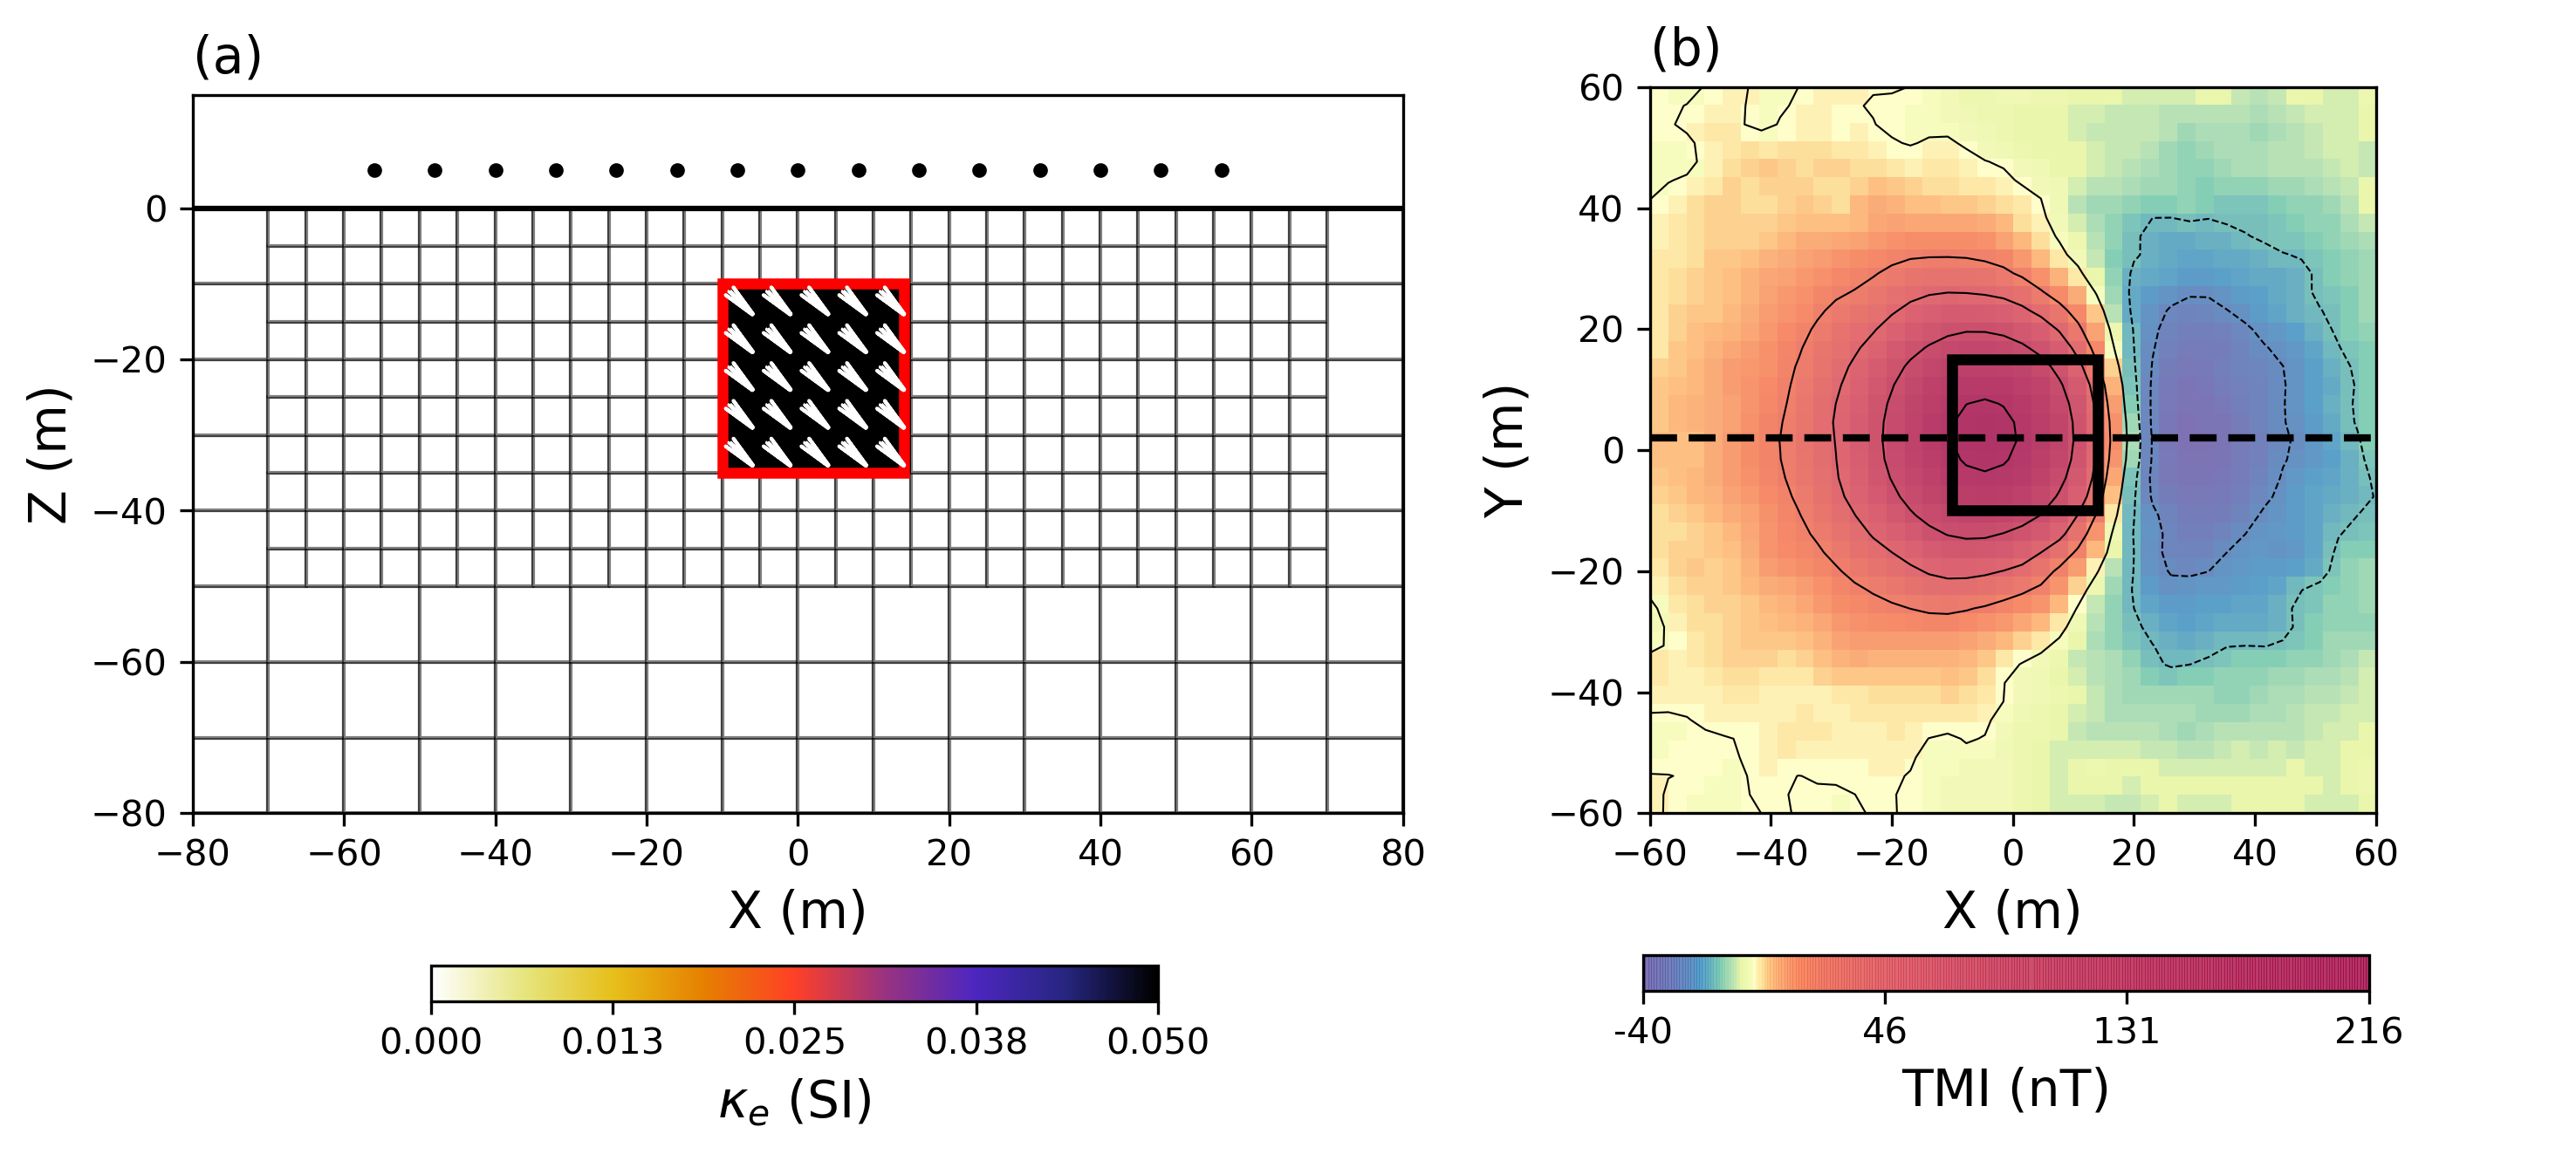
\includegraphics[width=\columnwidth]{Figures/Figure1.png}
\caption{(a) Vertical section through the synthetic block model (Y = 0 m) with magnetization $\mathbf{M}$ [$2.0\: A/m,\; I: 45^\circ,\; D: 90^\circ$]($\kappa_e$ = 0.05 SI). Survey points (black dots) are placed 15 m above the magnetic anomaly. (b) Simulated TMI data map with random Gaussian noise added, 1 nT standard deviation. The horizontal position of the block is shown in black for reference.}
\label{REM_model}
\end{figure}

\begin{figure}[p!]
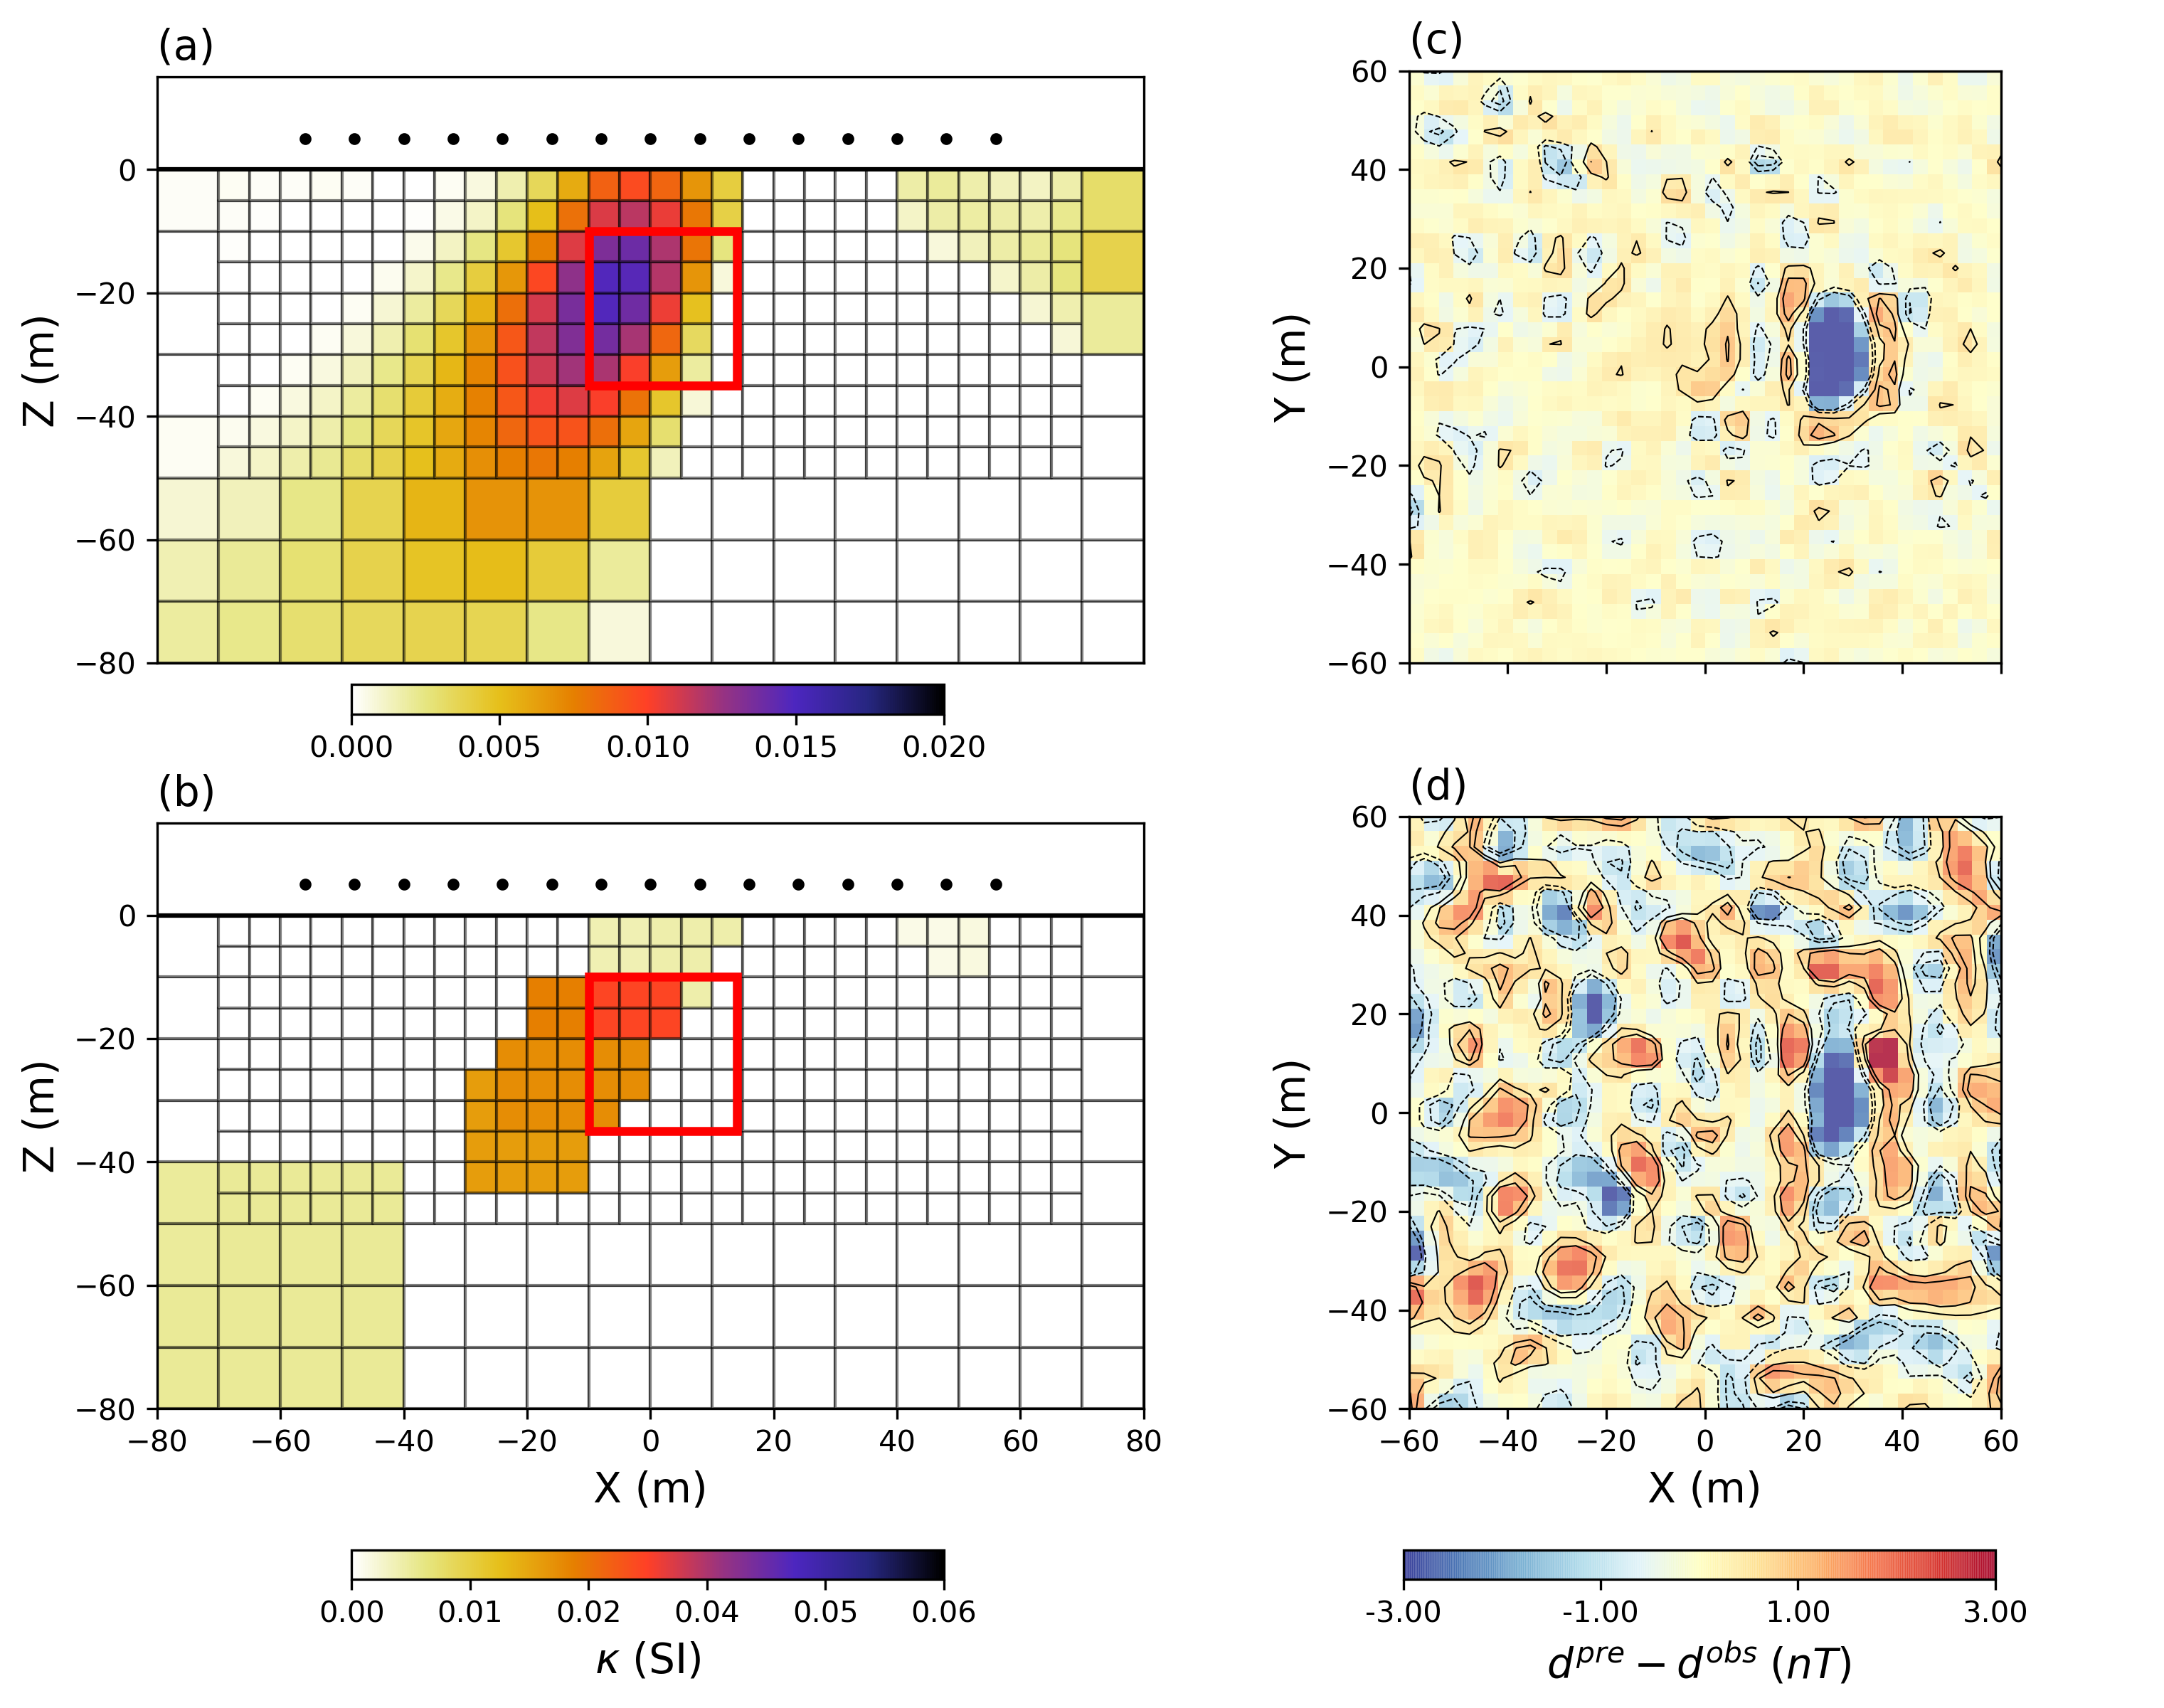
\includegraphics[width=\columnwidth]{Figures/Figure2.png}
\caption{Vertical section through the recovered susceptibility model using (a) smooth assumption ($p_s, \;p_x,\; p_y,\; p_z = 2$) and (b) sparse $\ell_p$-norms to recover a compact model ($p_s,\;p_x,\; p_y,\; p_z = 0$). Both solutions show an anomaly with a false dip due to the wrong assumption of a vertical magnetization. Data residuals for (c) the smooth and (d) compact solution shows correlated signal with the negative data.}\label{Susc_model}
\end{figure}

\begin{figure}[p!]
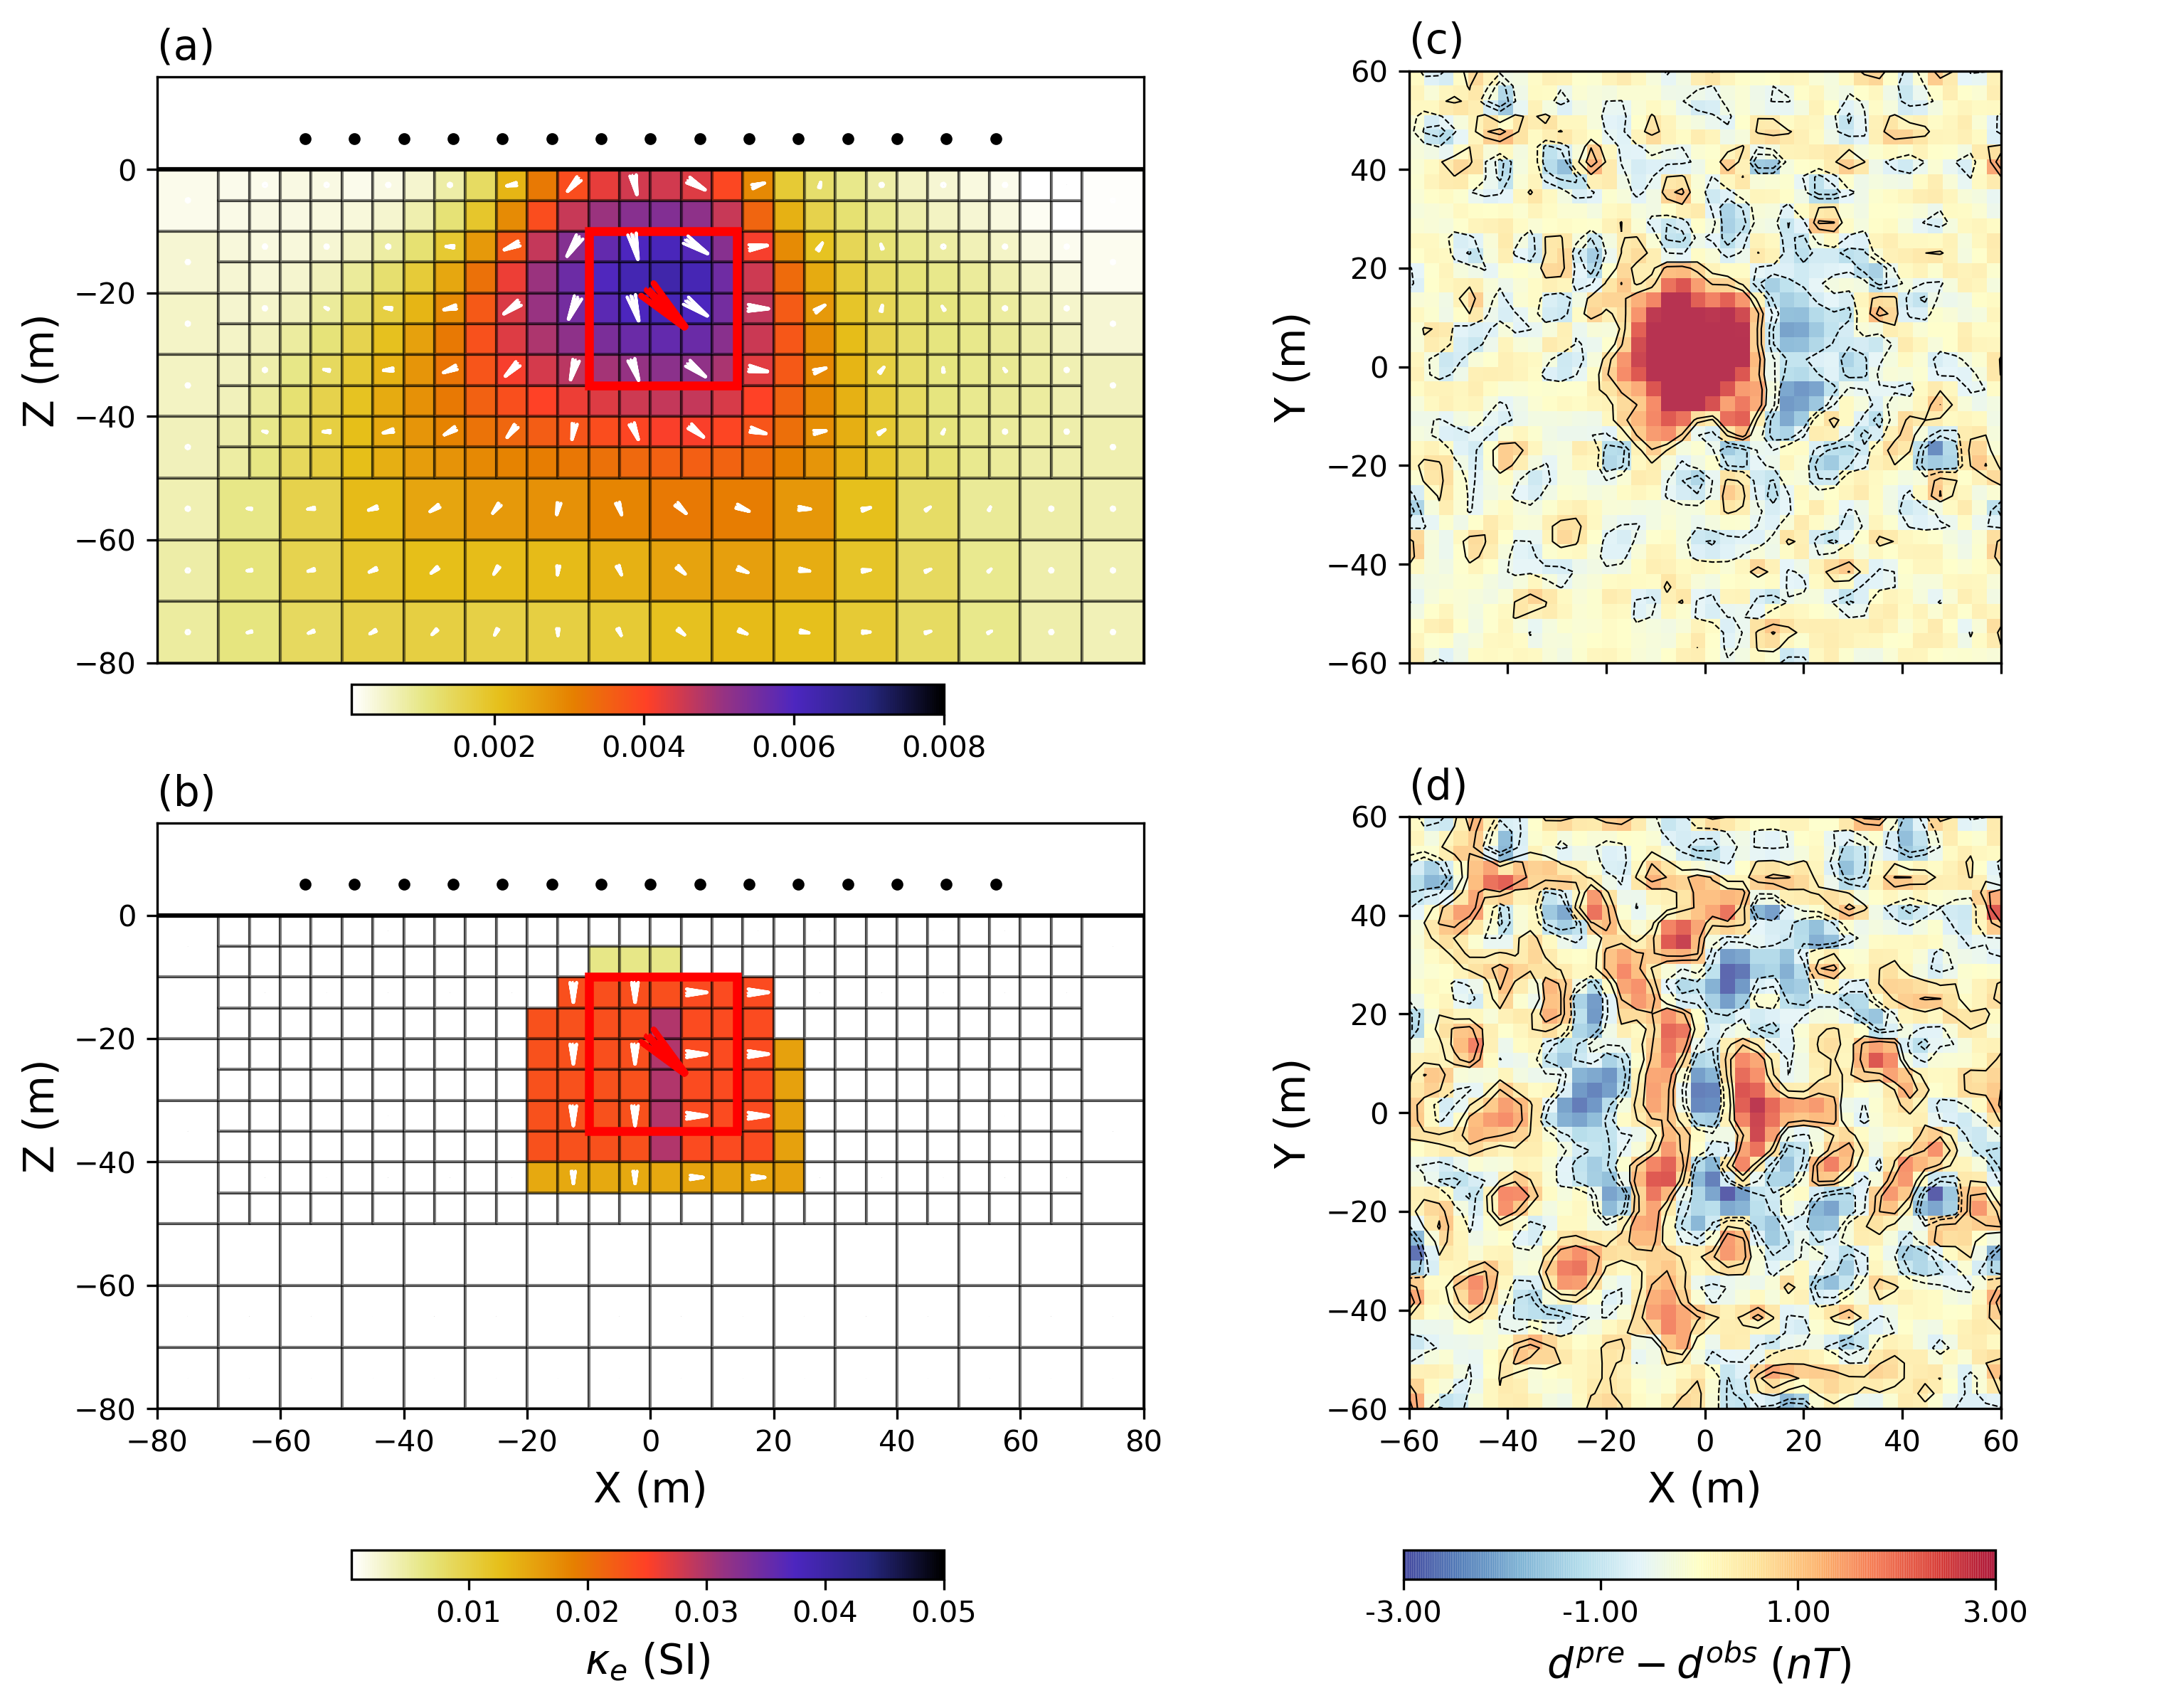
\includegraphics[width=\columnwidth]{Figures/Figure3.png}
\caption{Vertical section through the recovered magnetization vector model using the Cartesian formulation with (a) smooth $l_2$-norm assumption and (b) sparsity constraints applied on all three Cartesian components ($p_{i_s}, \;p_{i_x},\; p_{i_y},\; p_{i_z} = 0$). Color is scaled by the magnitude of magnetization. The true magnetization direction is shown with a red arrow. Data residual map calculated with (c) the smooth and (d) compact solution.}
\label{MVI_C_model}
\end{figure}

\begin{figure}[p!]
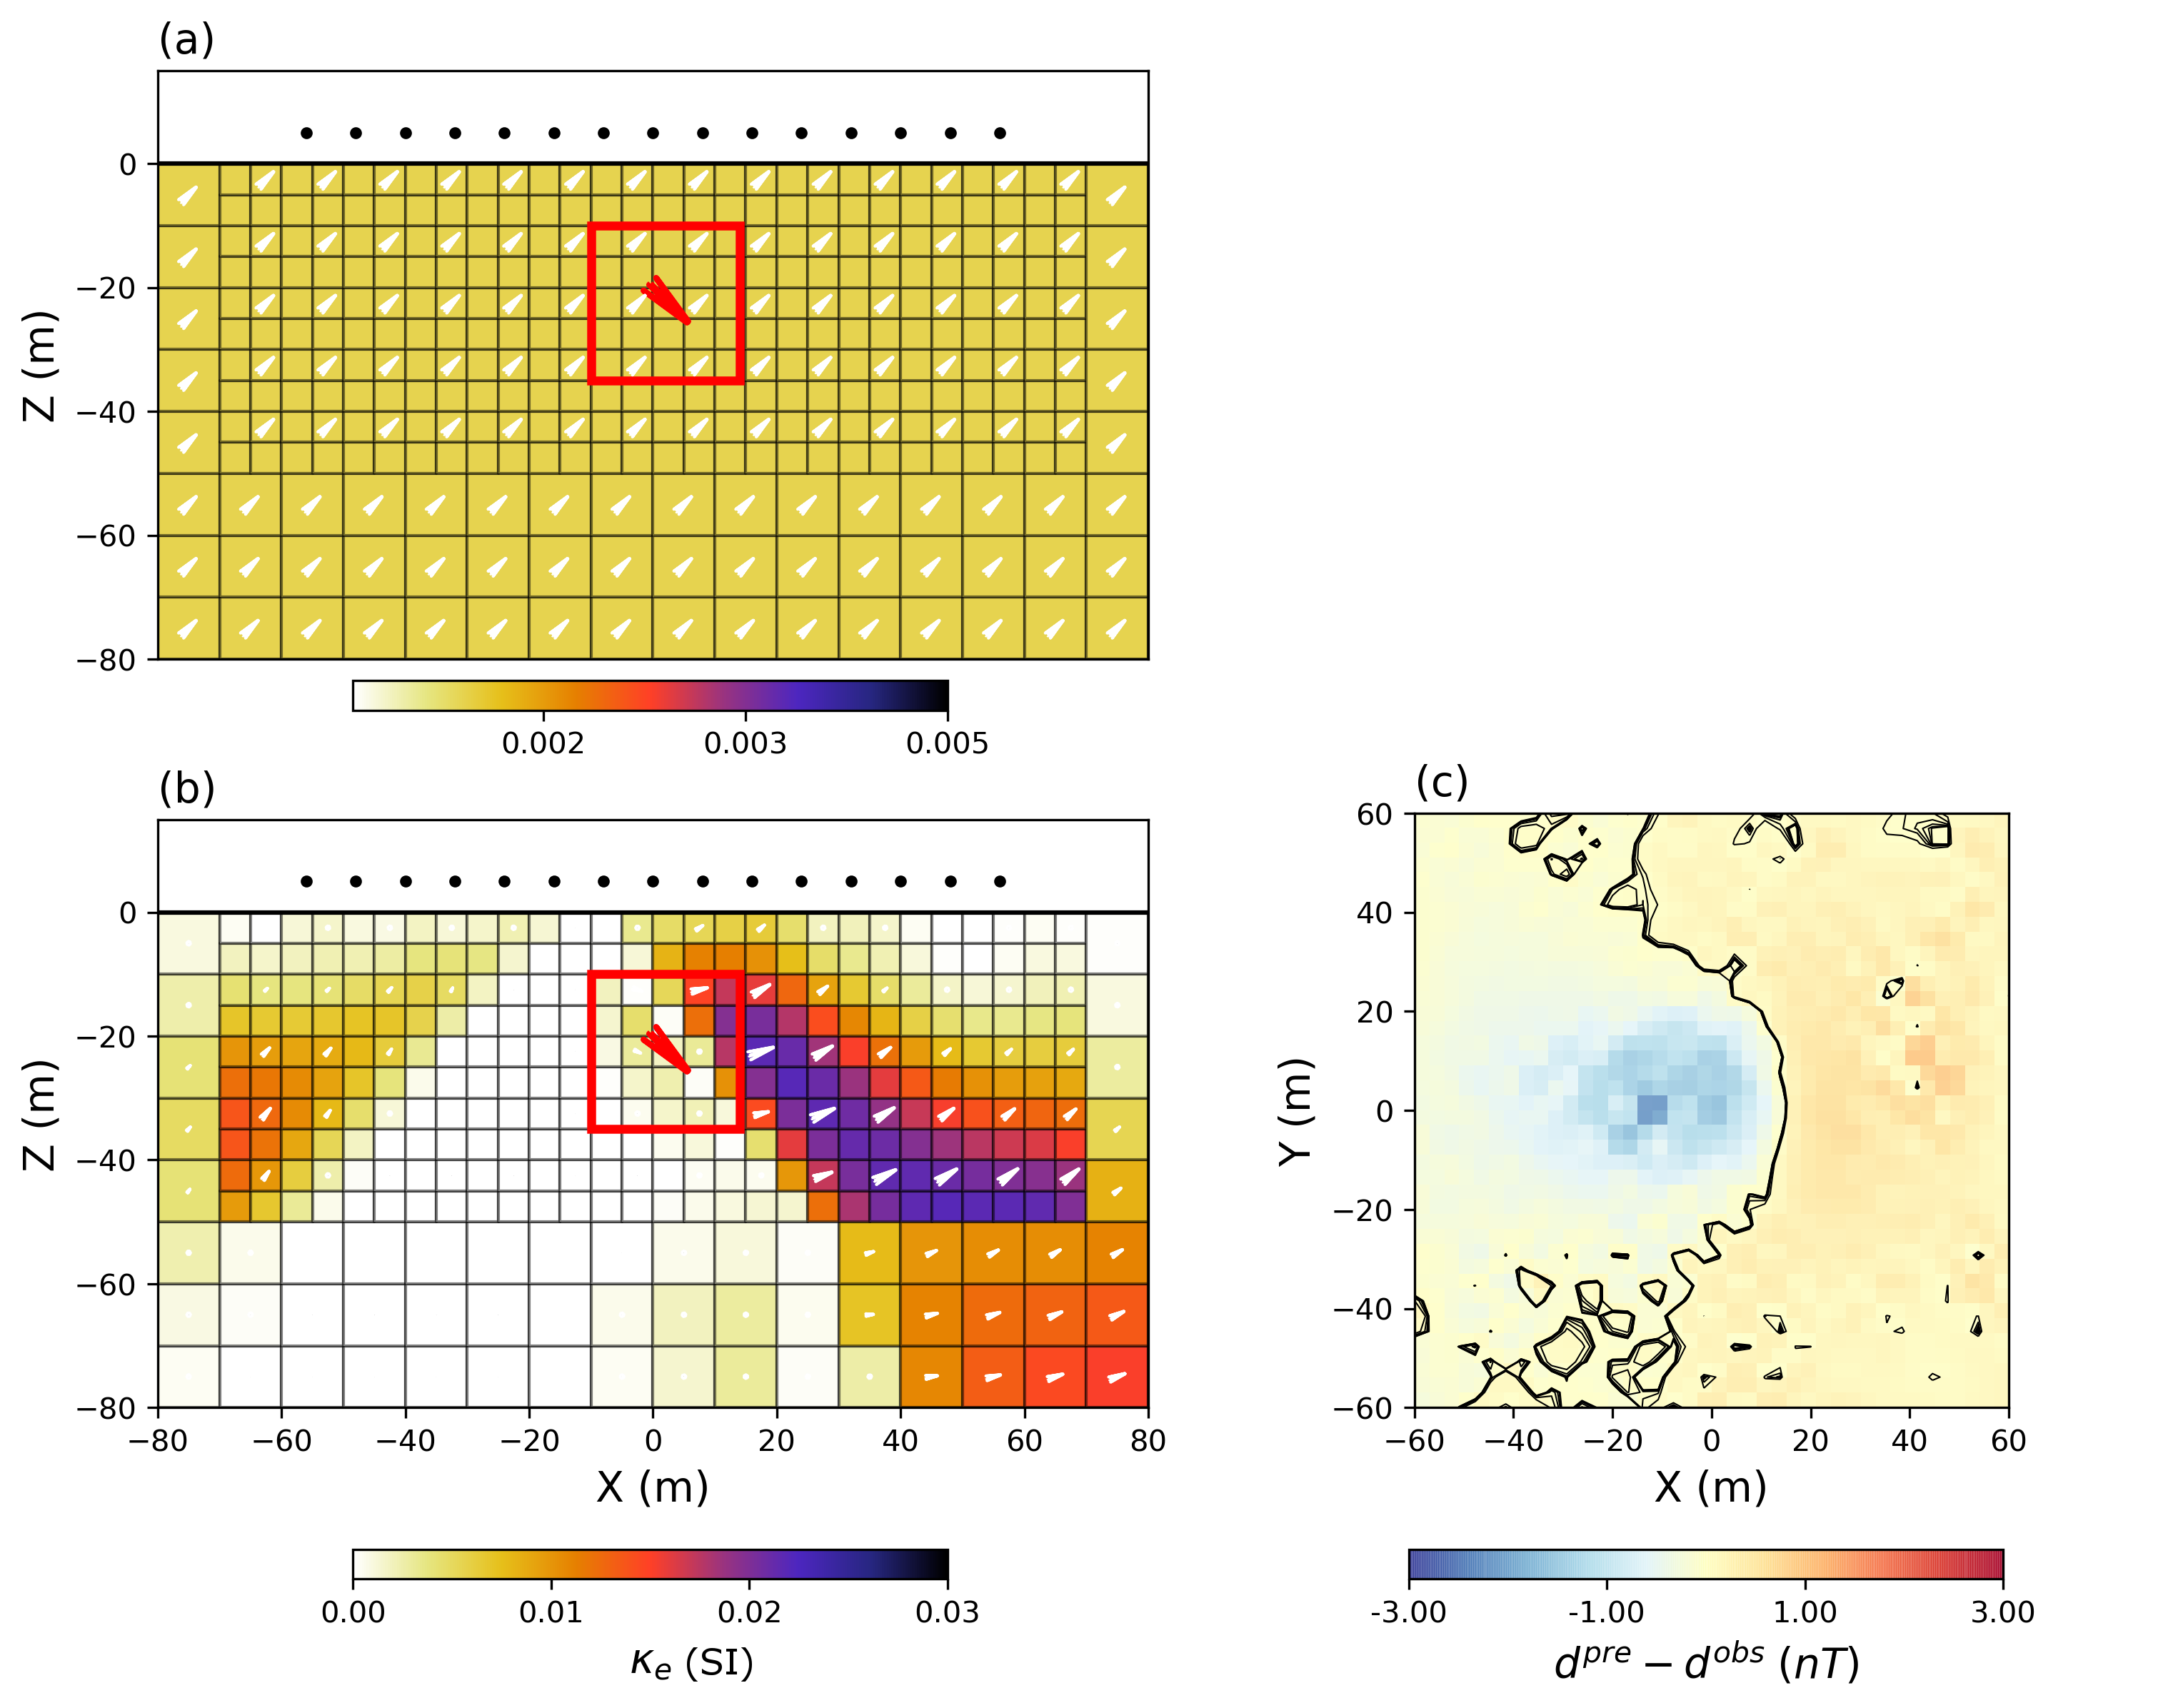
\includegraphics[width=\columnwidth]{Figures/Figure4.png}
\caption{ Vertical section through the (a) starting model and (b) recovered magnetization vector model in spherical coordinates with its (c) data residual map. The inversion stopped after three iterations, unable to further reduce the objective function.}
\label{MVI_S_model_noScale}
\end{figure}

\begin{figure}[p!]
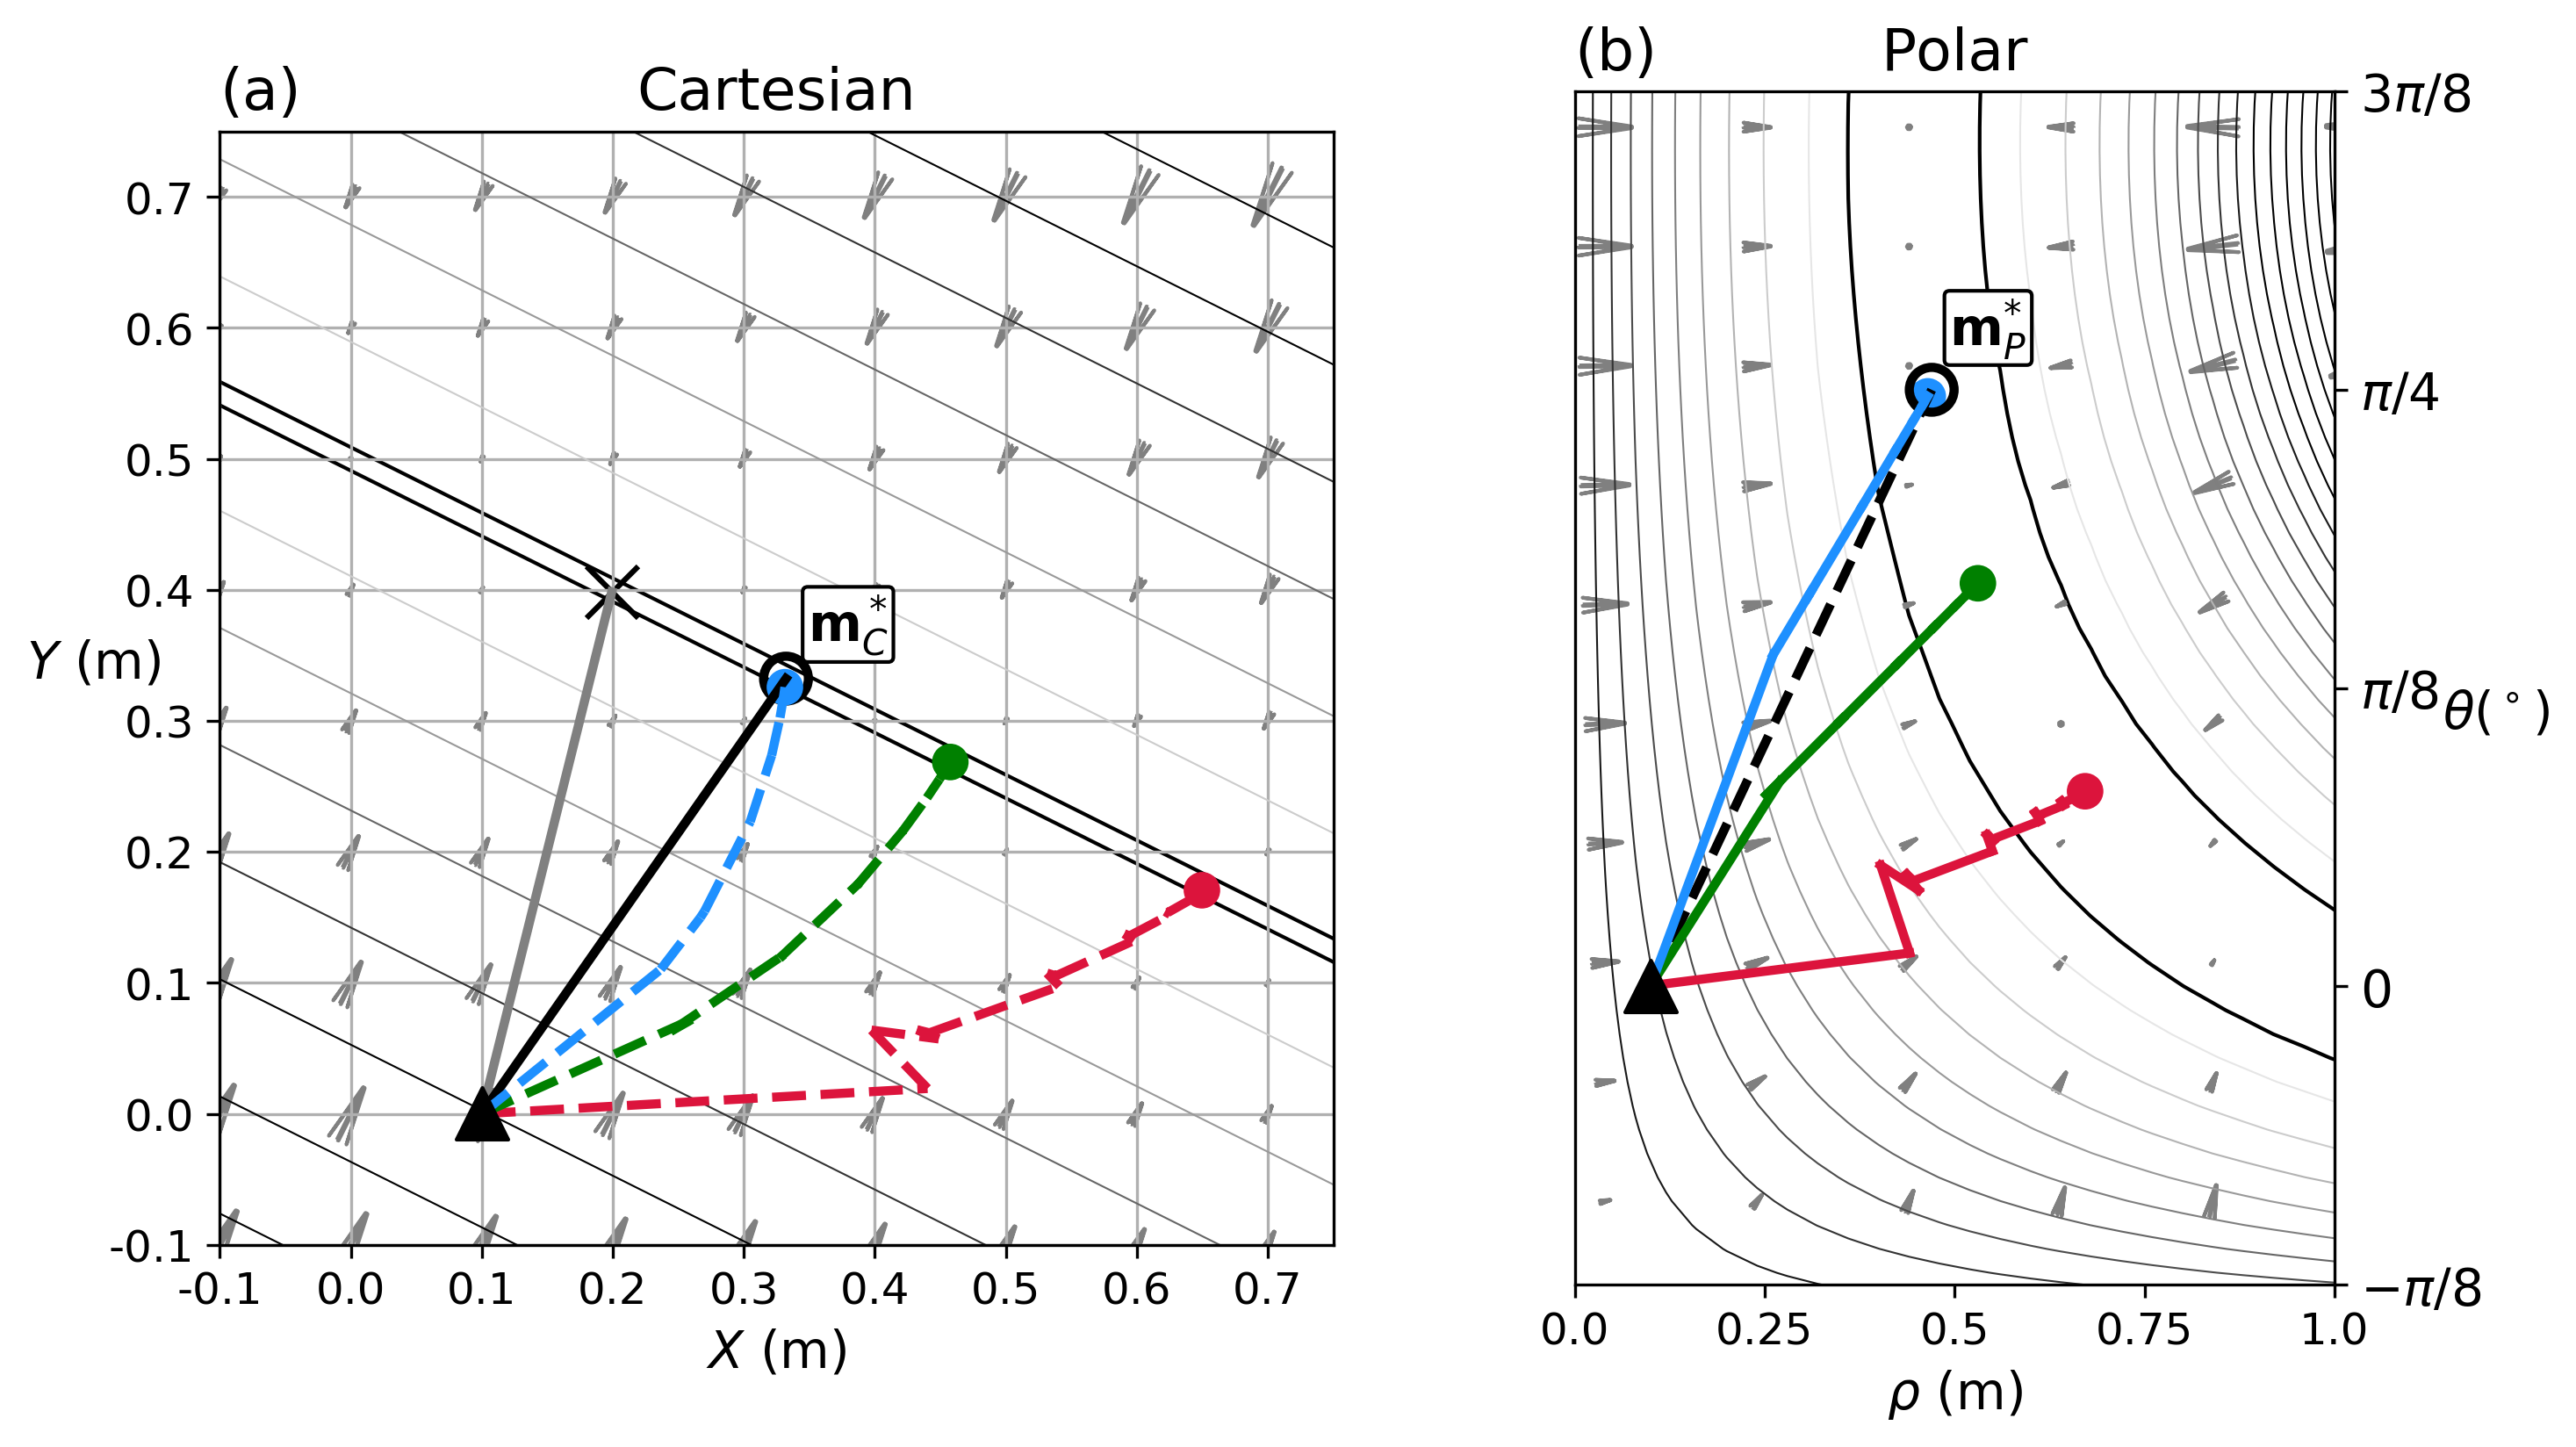
\includegraphics[width=\columnwidth]{Figures/Figure5.png}
\caption{Contour maps for the objective functions of a two-parameter inverse problem solved in (a) Cartesian and (b) polar coordinate systems. Solid colored lines show the model updates taken by different algorithms in their respective coordinate systems and, in dash, the equivalent steps in the other domain for comparison. Each inversion started with the same initial model (triangle). The colors and inversions are: Gray: the non-weighted Cartesian problem; Black: the sensitivity weighted Cartesian problem; Red: the non-linear polar coordinate system with fixed sensitivity weights; Green: the polar problem with iterative sensitivity re-weighting; and Blue: with the added scaling to compensate for the dynamic range of the parameters (see equation~50). }
\label{NonLinearGN}
\end{figure}

\begin{figure}[p!]
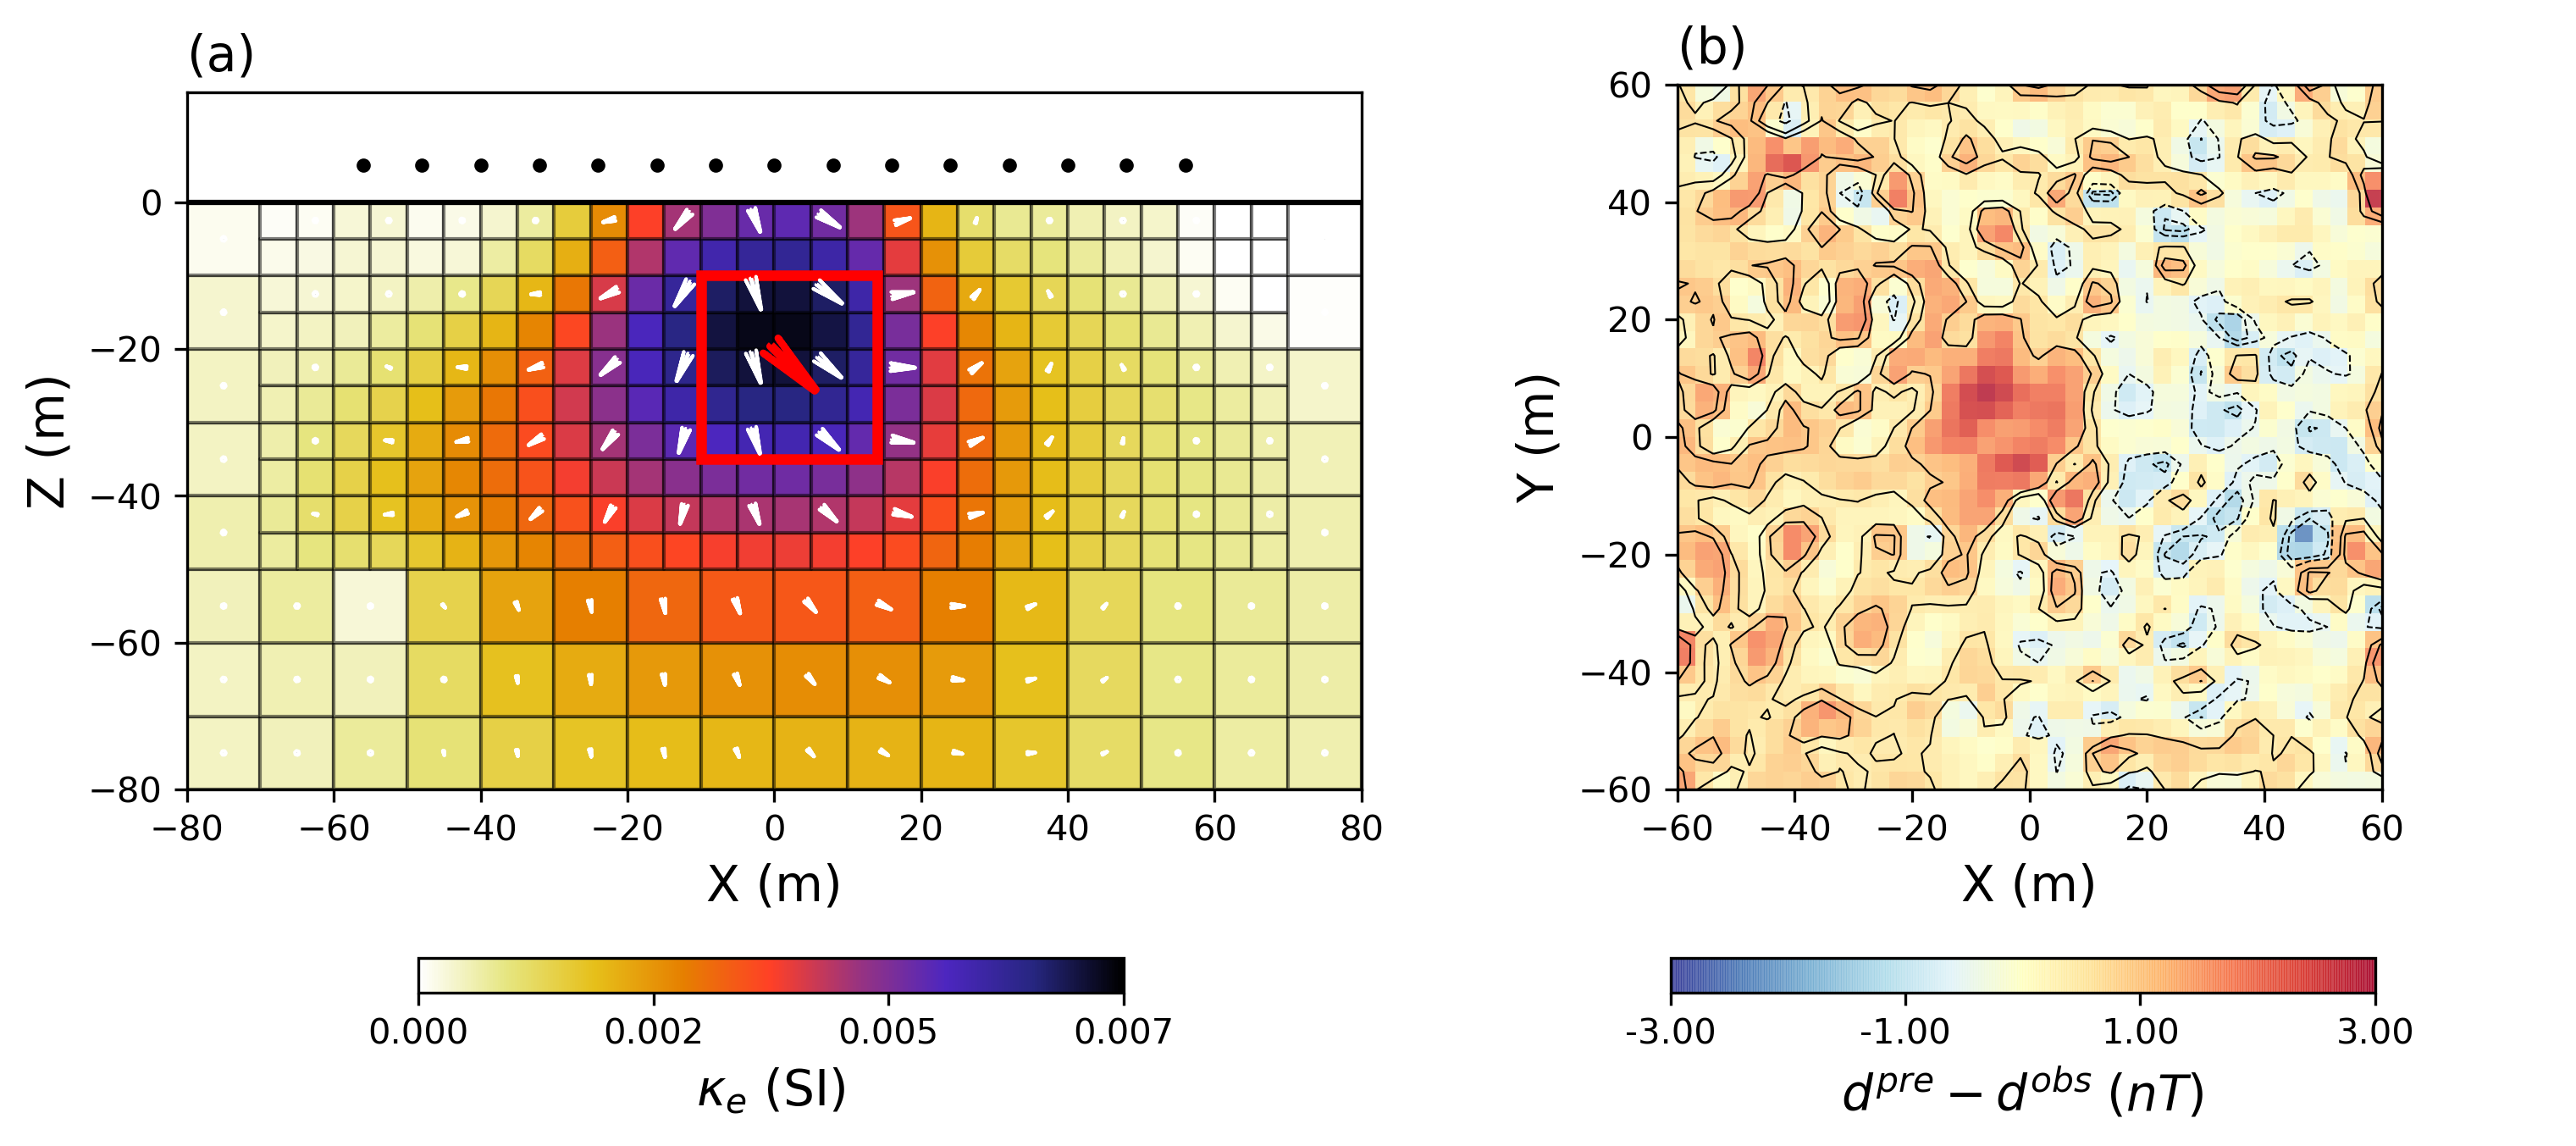
\includegraphics[width=\columnwidth]{Figures/Figure6.png}
\caption{(a) Vertical section through the recovered magnetization vector model in spherical coordinates using sensitivity based weighting and (b) the corresponding data residual map. The same poor starting model shown in Figure~\ref{MVI_S_model_noScale}a was used, but the algorithm converged to a solution similar to the Cartesian solution.}
\label{MVI_S_model}
\end{figure}

\begin{figure}[p!]
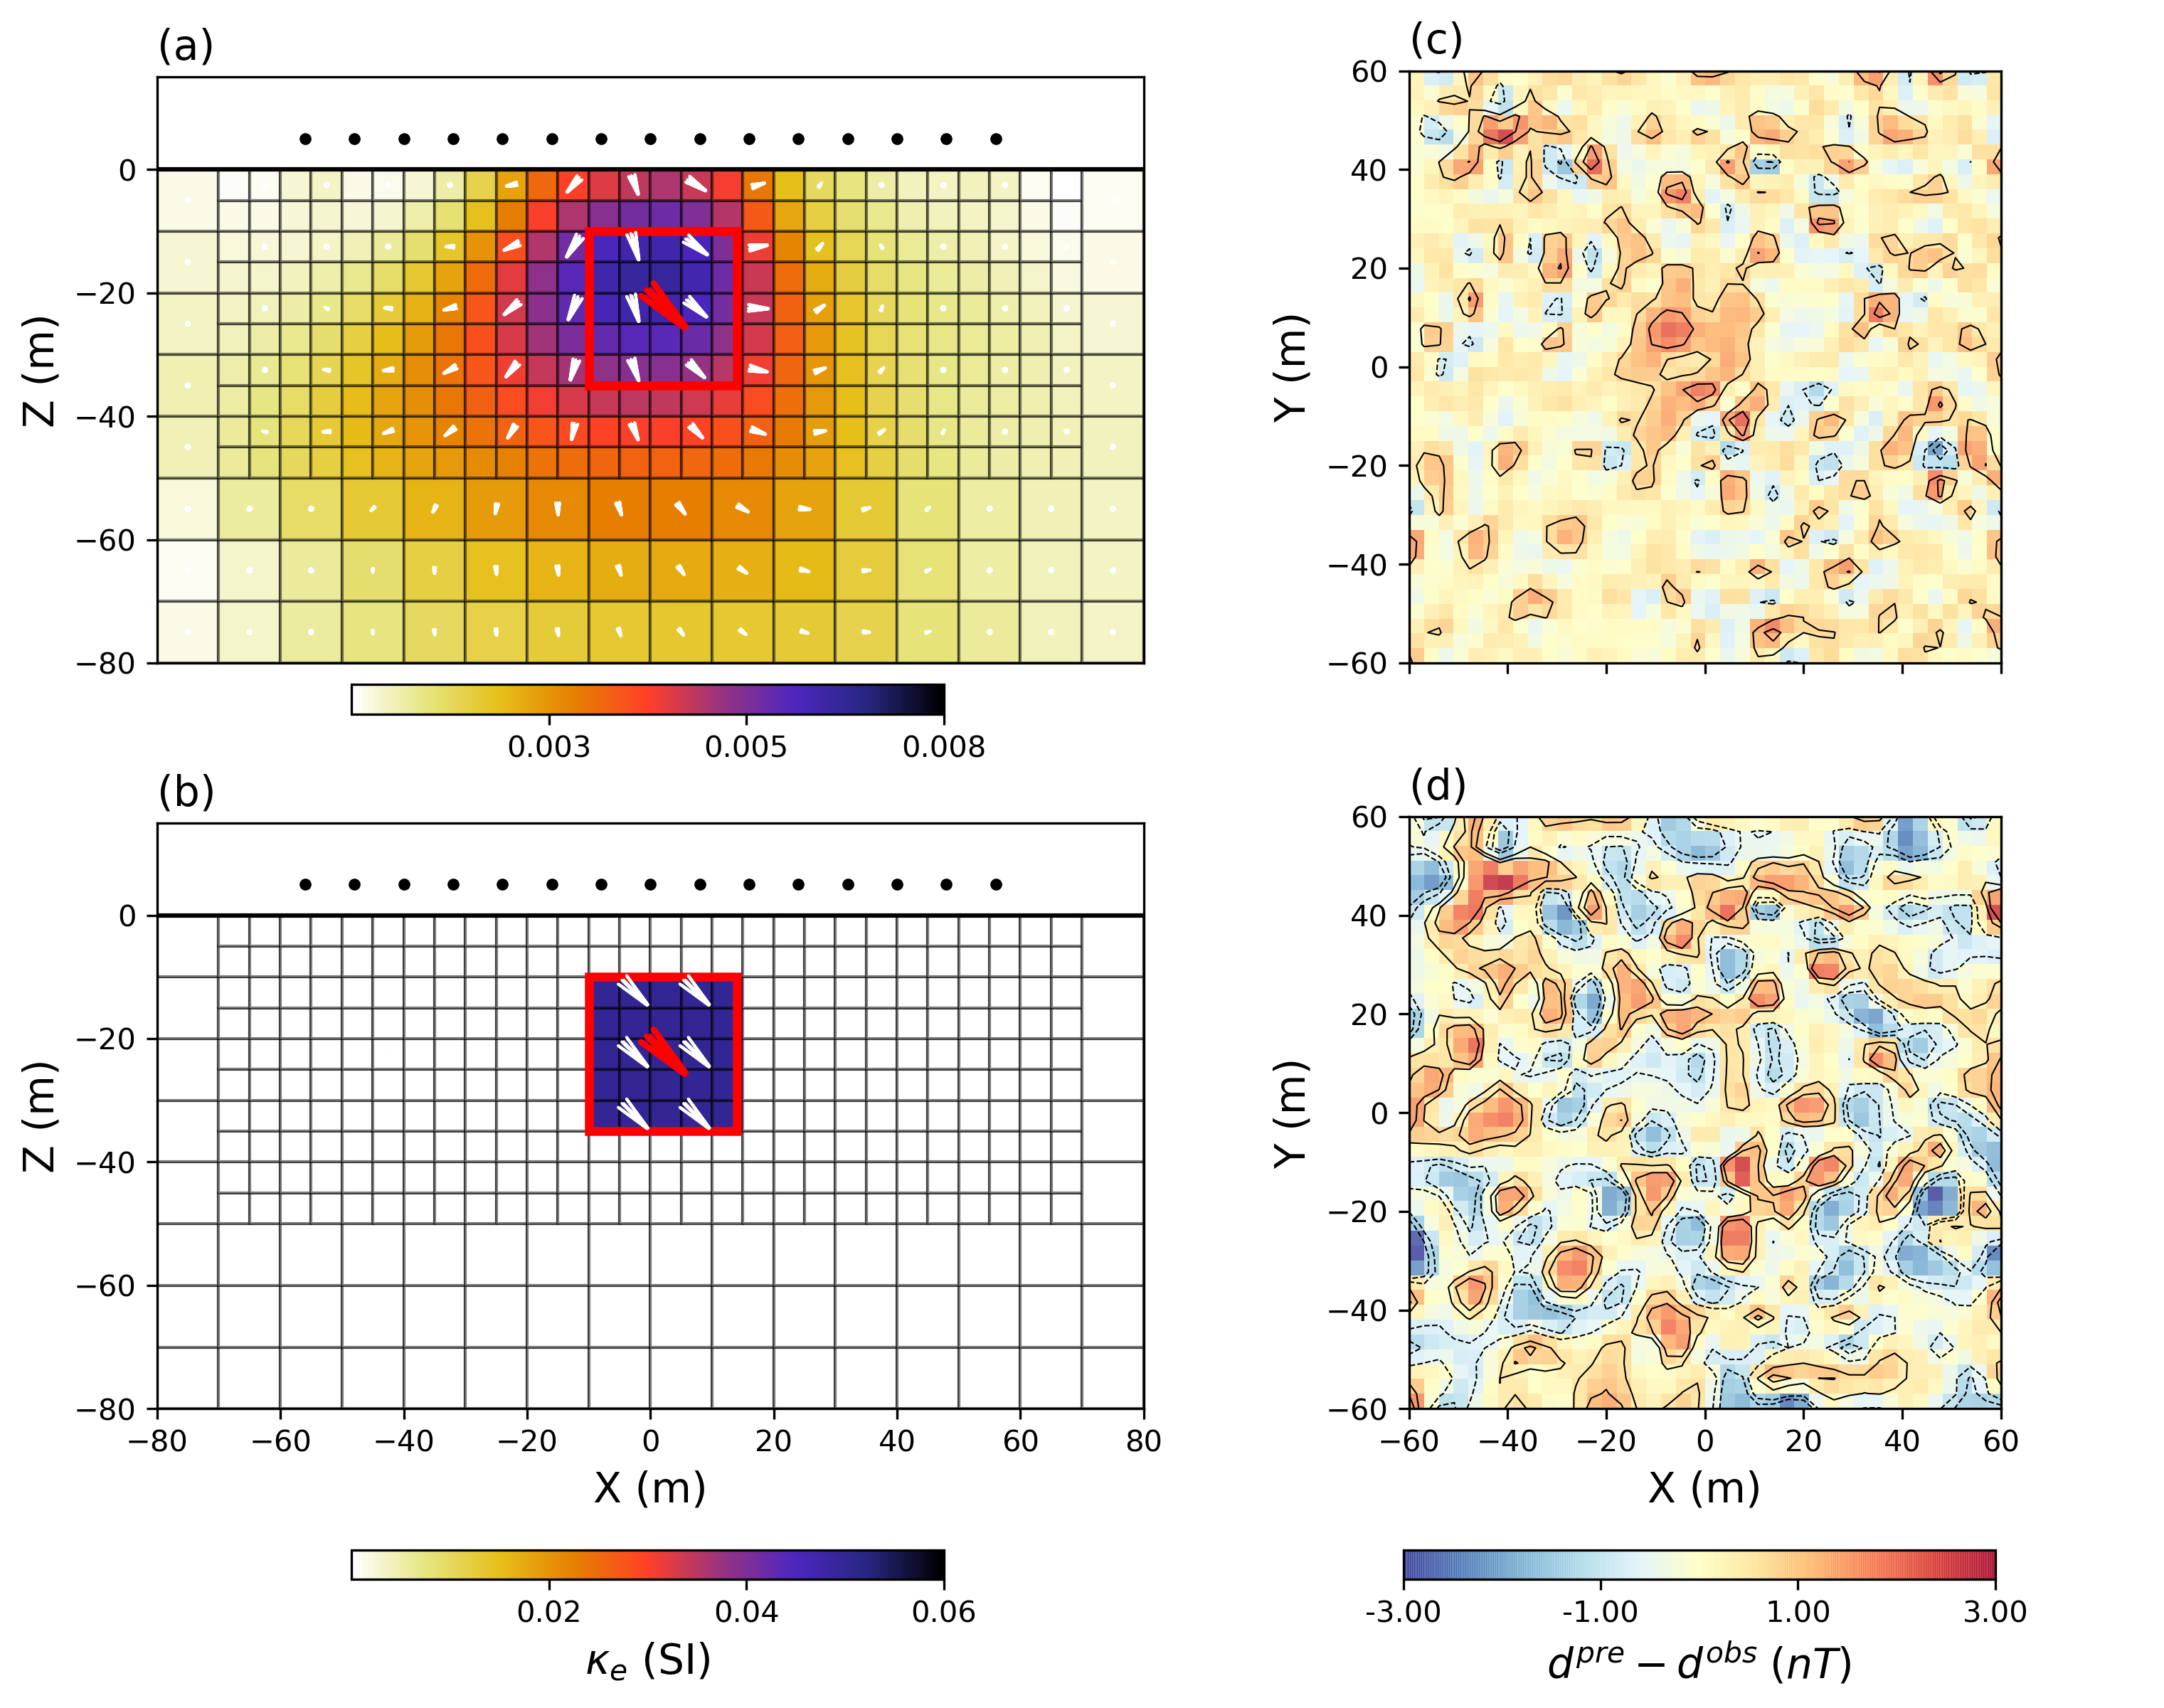
\includegraphics[width=\columnwidth]{Figures/Figure7.png}
\caption{Vertical section through the recovered magnetization vector model in spherical coordinates using sensitivity based weighting and the smooth Cartesian solution as starting model: (a) smooth regularization ($p_s=p_x=p_y=p_z = 2$) and (b) sparse norms on the strength and angles of the magnetization vector ($p_s=p_x=p_y=p_z = 0$). By using the sparse norms, we recover a solution that closely resembles the true model and, as observed in (d), we also eliminate the coherent signal in the residual data that is observed in (c).}
\label{MVI_S_model_lp}
\end{figure}

\begin{figure}[p!]
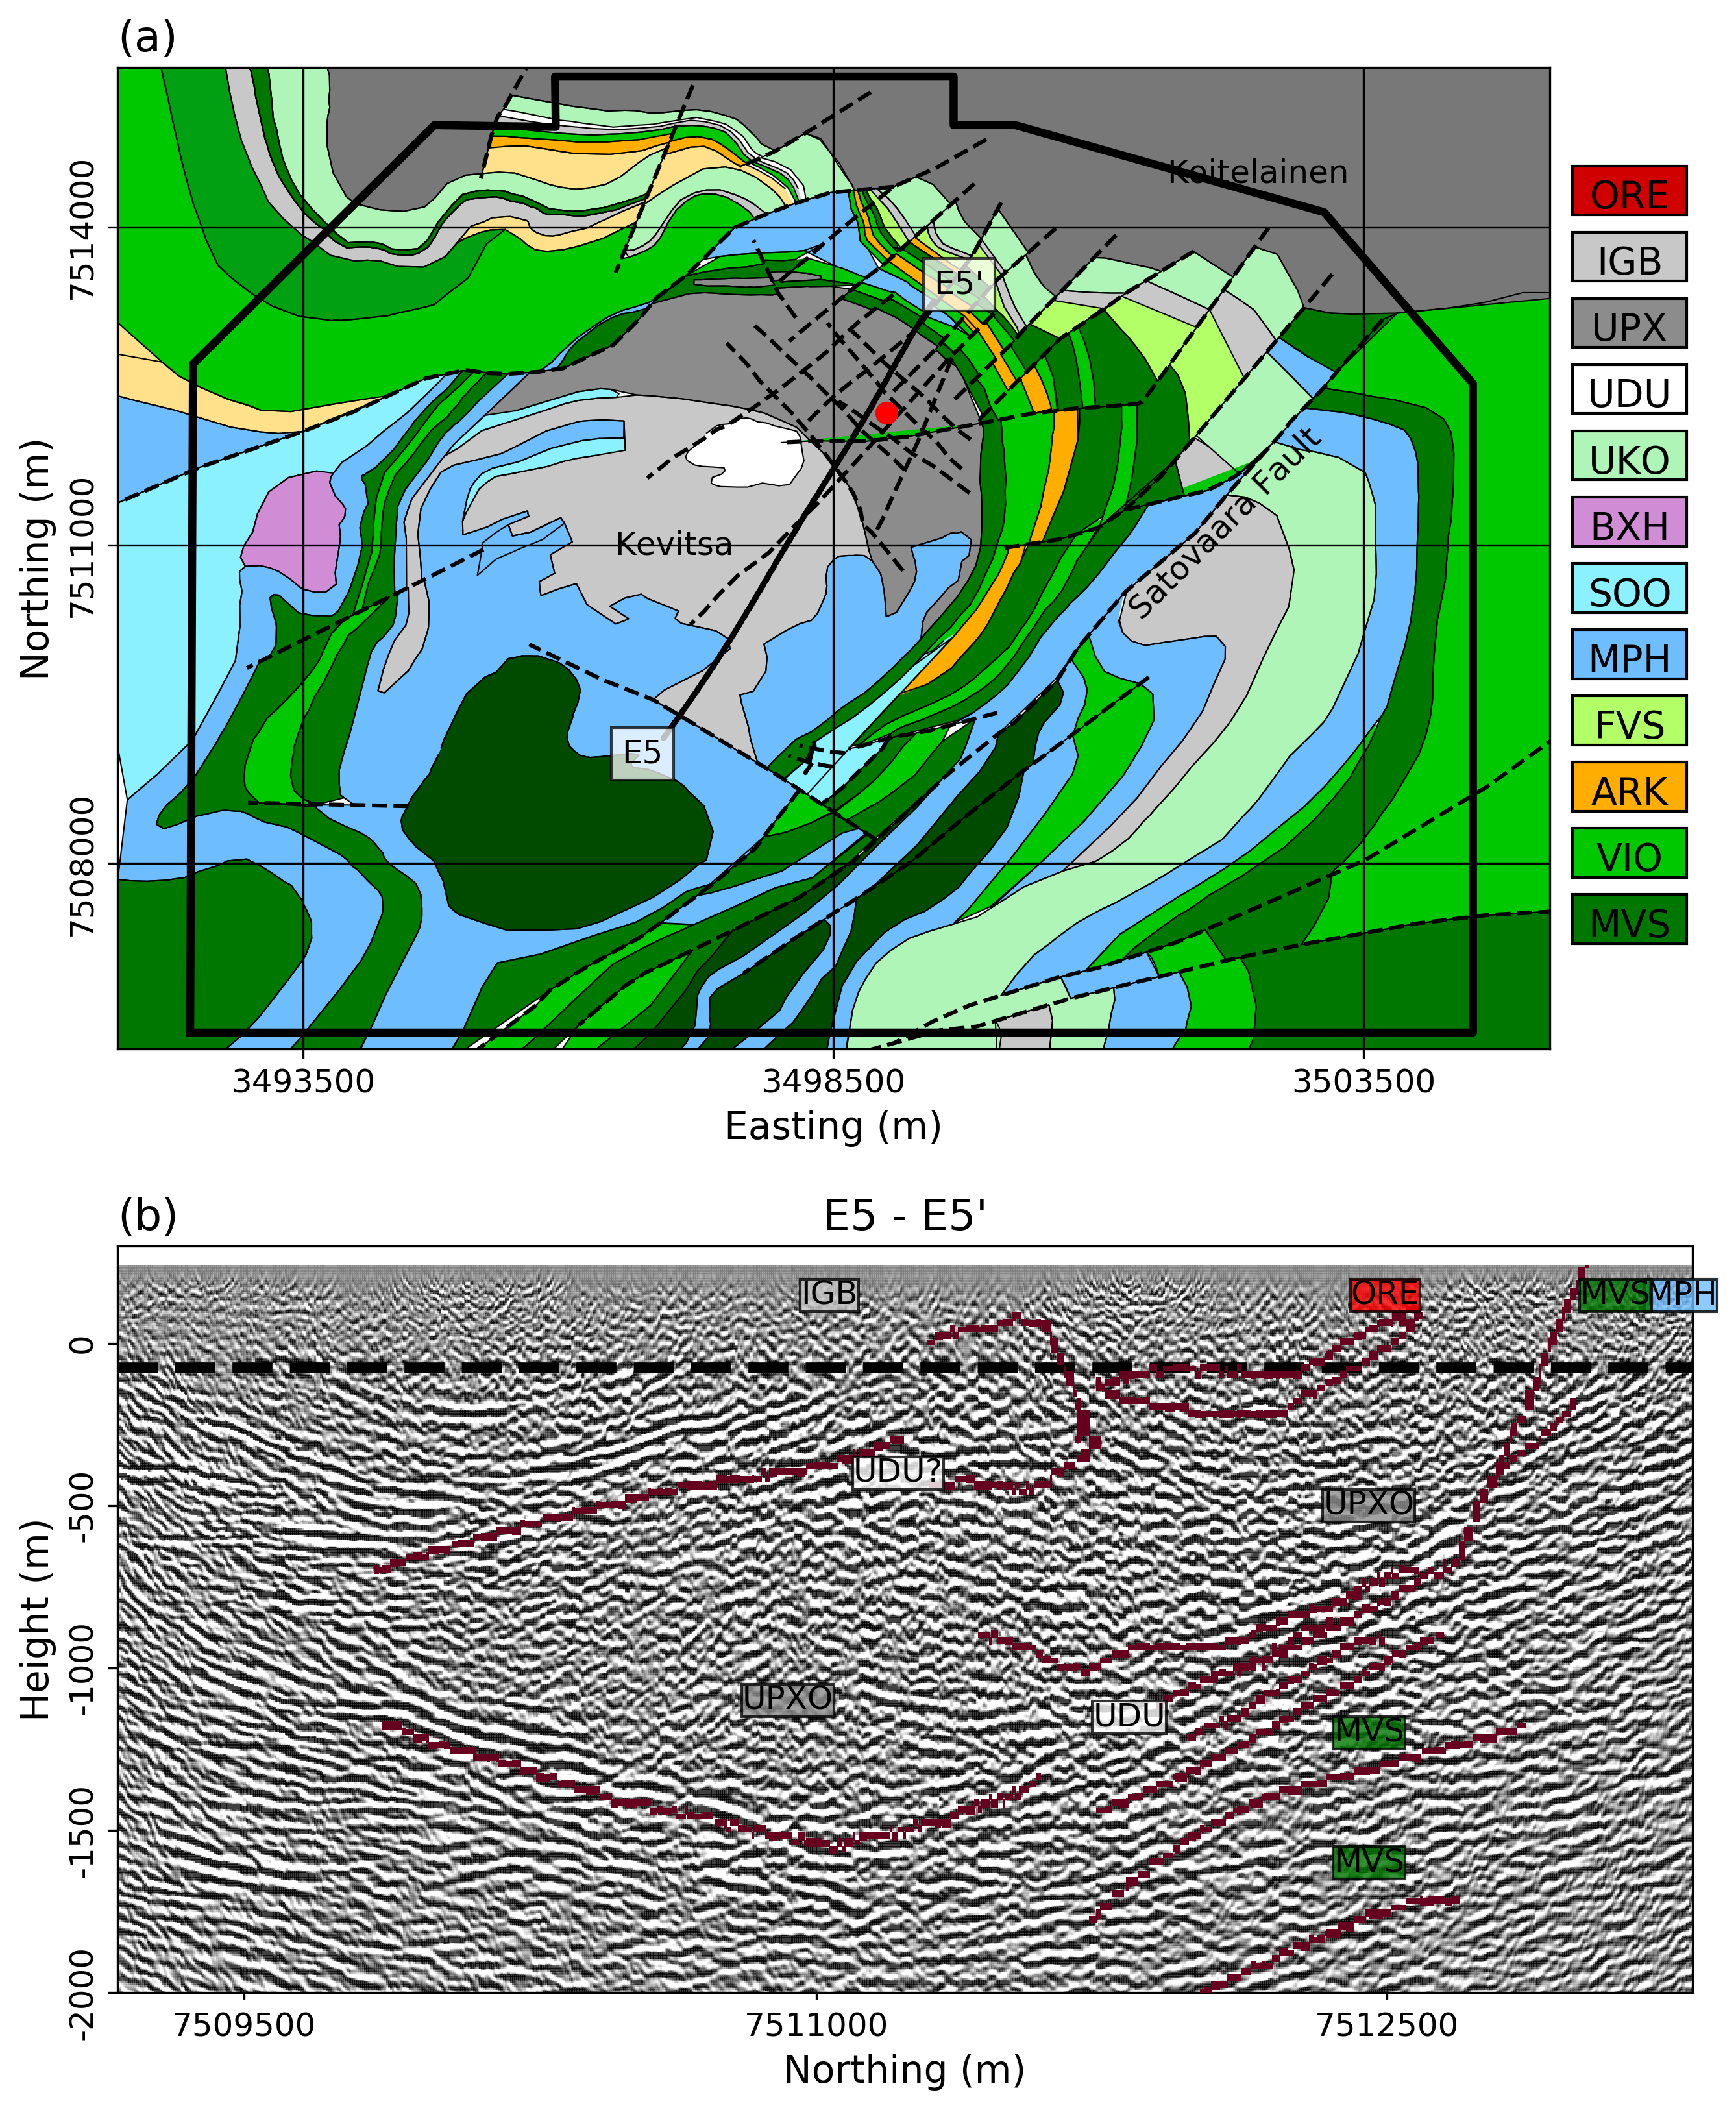
\includegraphics[width=\columnwidth]{Figures/Figure8.png}
\caption{(a) Geological map of the Kevitsa-Satovaara intrusive complex adapted from \cite{Koivisto2015}, with geological definition provided in Table~1. Mapped faults (dash) are shown for reference. (b) 2D seismic line reflection line E5 with interpreted geological contacts between the main reflectors.}
\label{Kevitsa_Geology}
\end{figure}

\begin{figure}[p!]
%\includegraphics[width=0.5\columnwidth]{Figure9.png}
\caption{Whisker plot of magnetic susceptibility measured along 279 boreholes. The coloured boxes have a width scaled by the calculated standard deviation and centered on the mean value for all intercepts belonging to the same lithological classification, as defined in Table~1. The black lines on either side define the minimum and maximum values. The different lithologies are colour coded and grouped based on relative age and similarities in physical properties.}
\label{Kevitsa_PhysProp}
\end{figure}

\begin{figure}[p!]
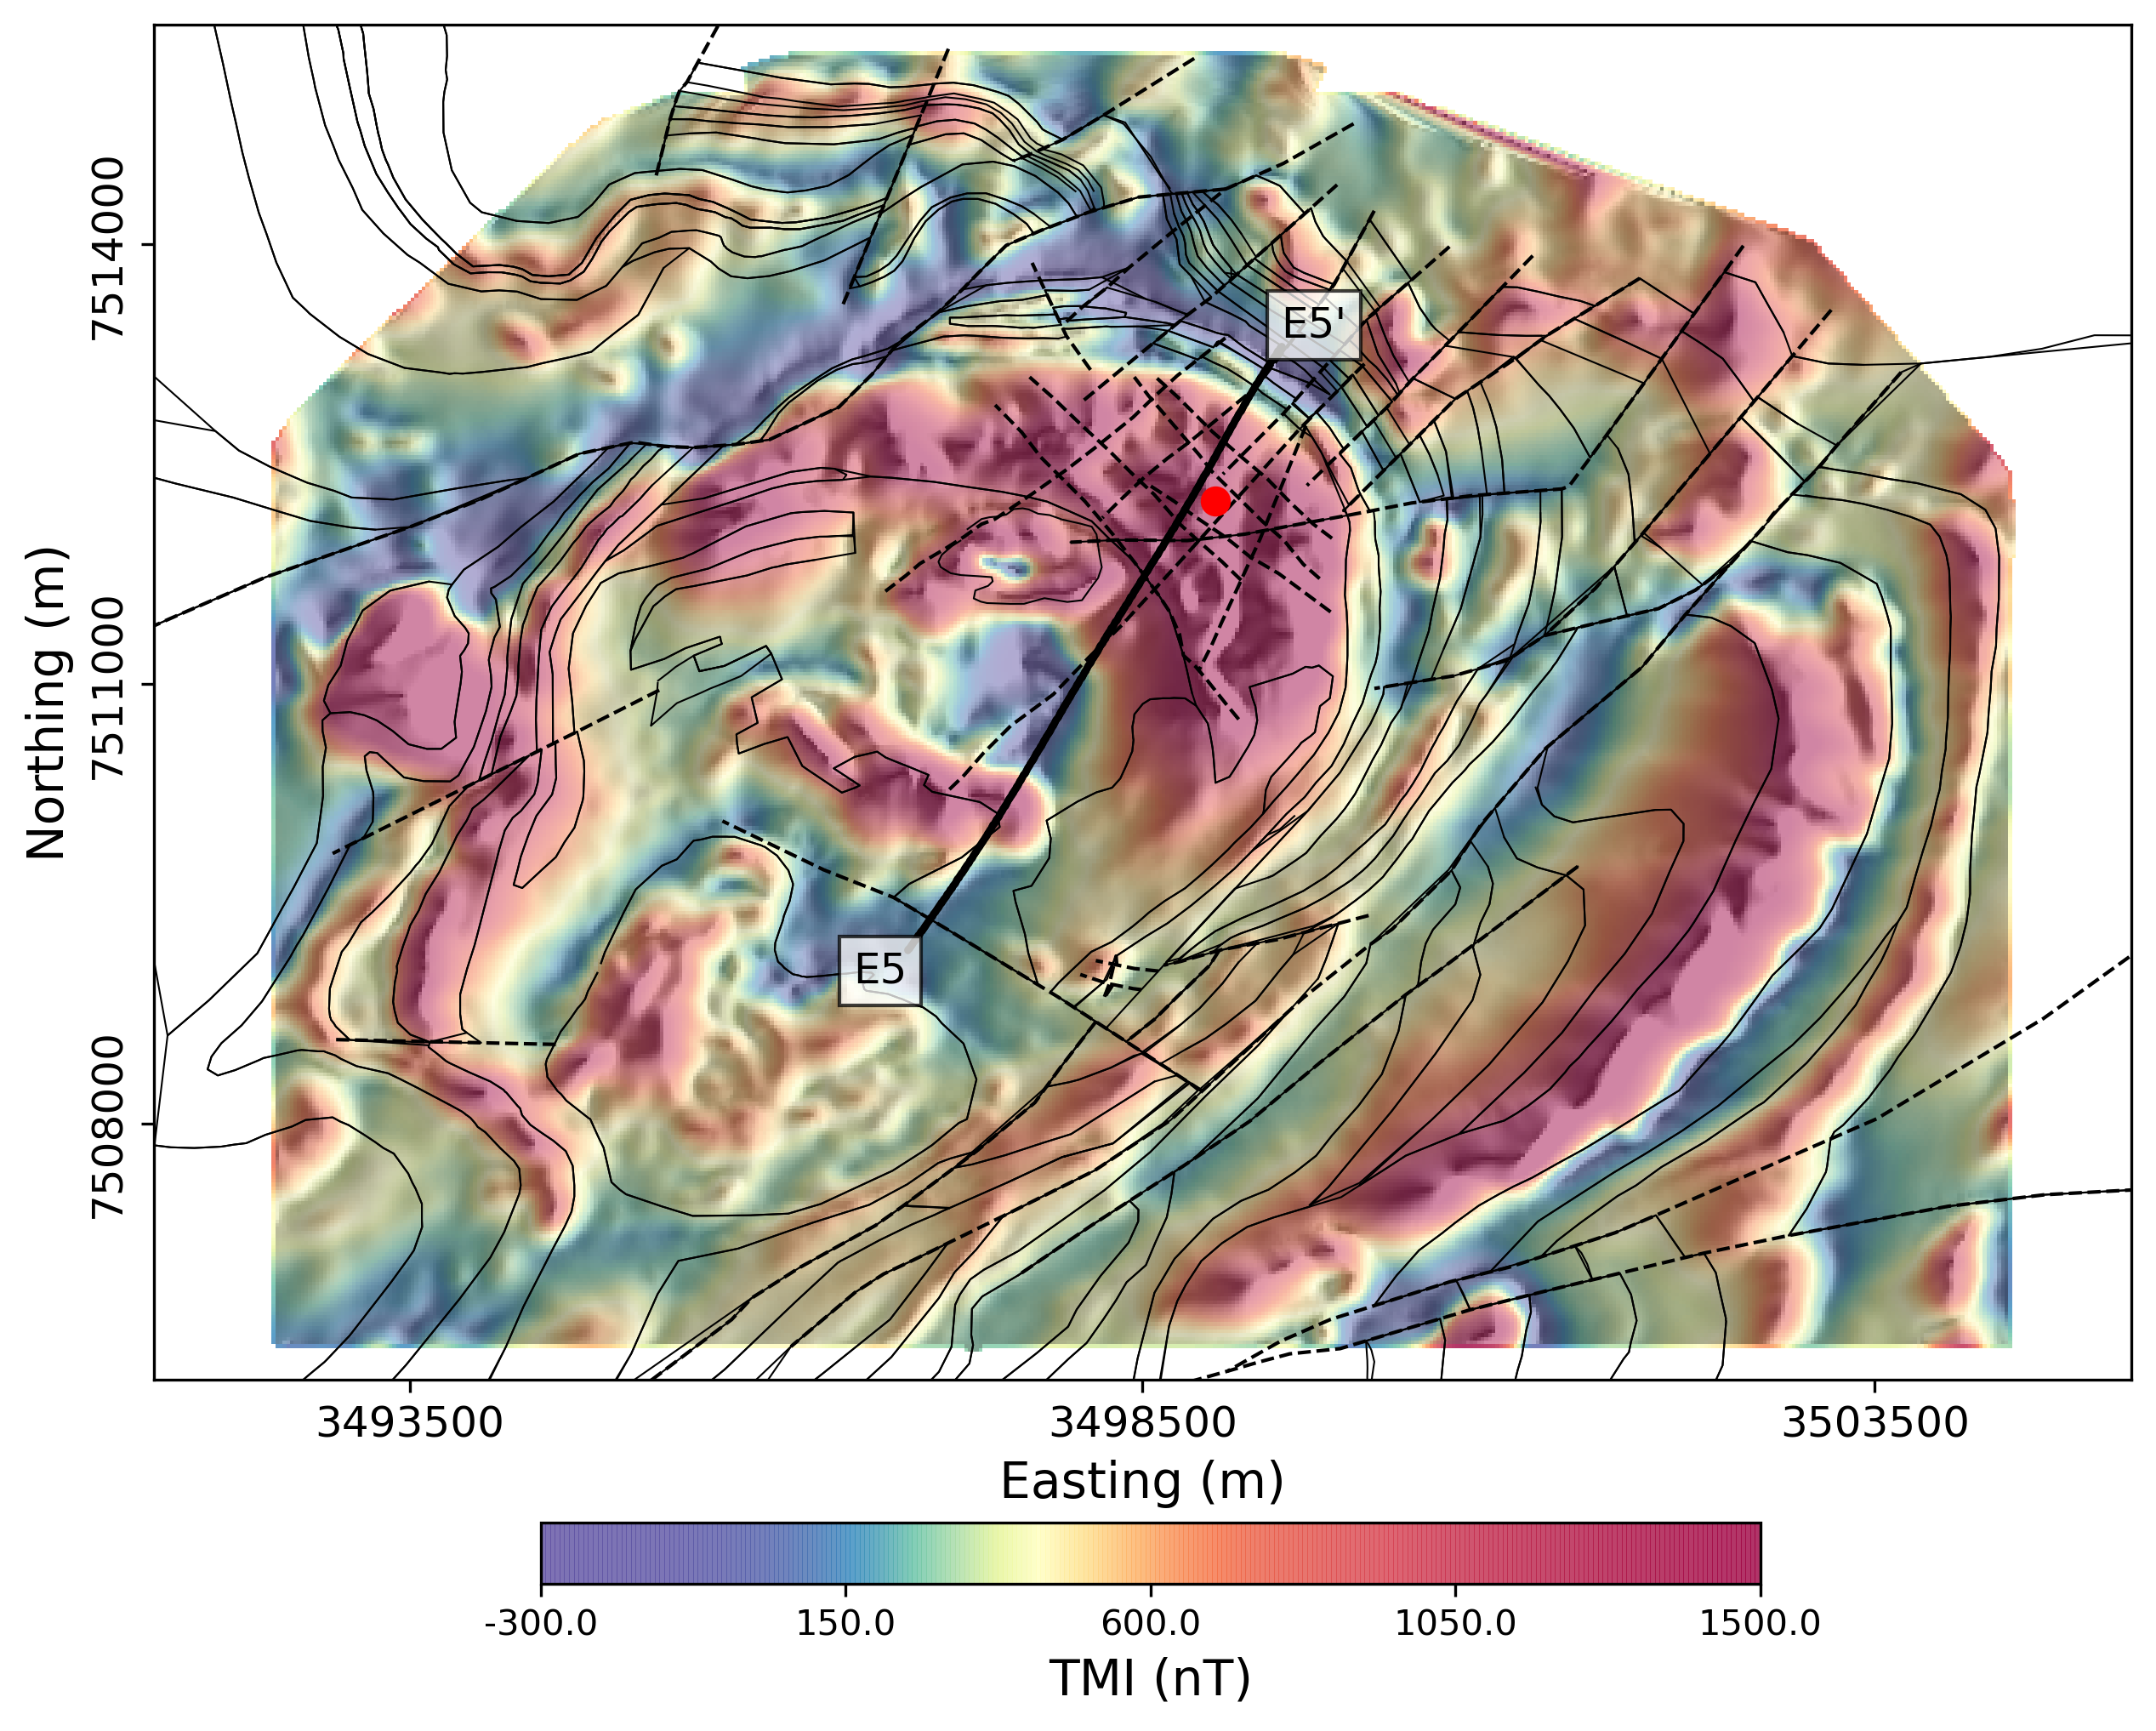
\includegraphics[width=\columnwidth]{Figures/Figure10.png}
\caption{Observed TMI data over the Kevitsa intrusion with histogram equalized color scale. Geological contacts (black), faults (dash) identified from surface mapping and the 2D seismic line locations E5, are shown for reference. Sun shading from east is added to highlight subtle features (Azimuth: $270^\circ$, Dip: $45^\circ$).}
\label{Kevitsa_TMI}
\end{figure}

\begin{figure}[p!]
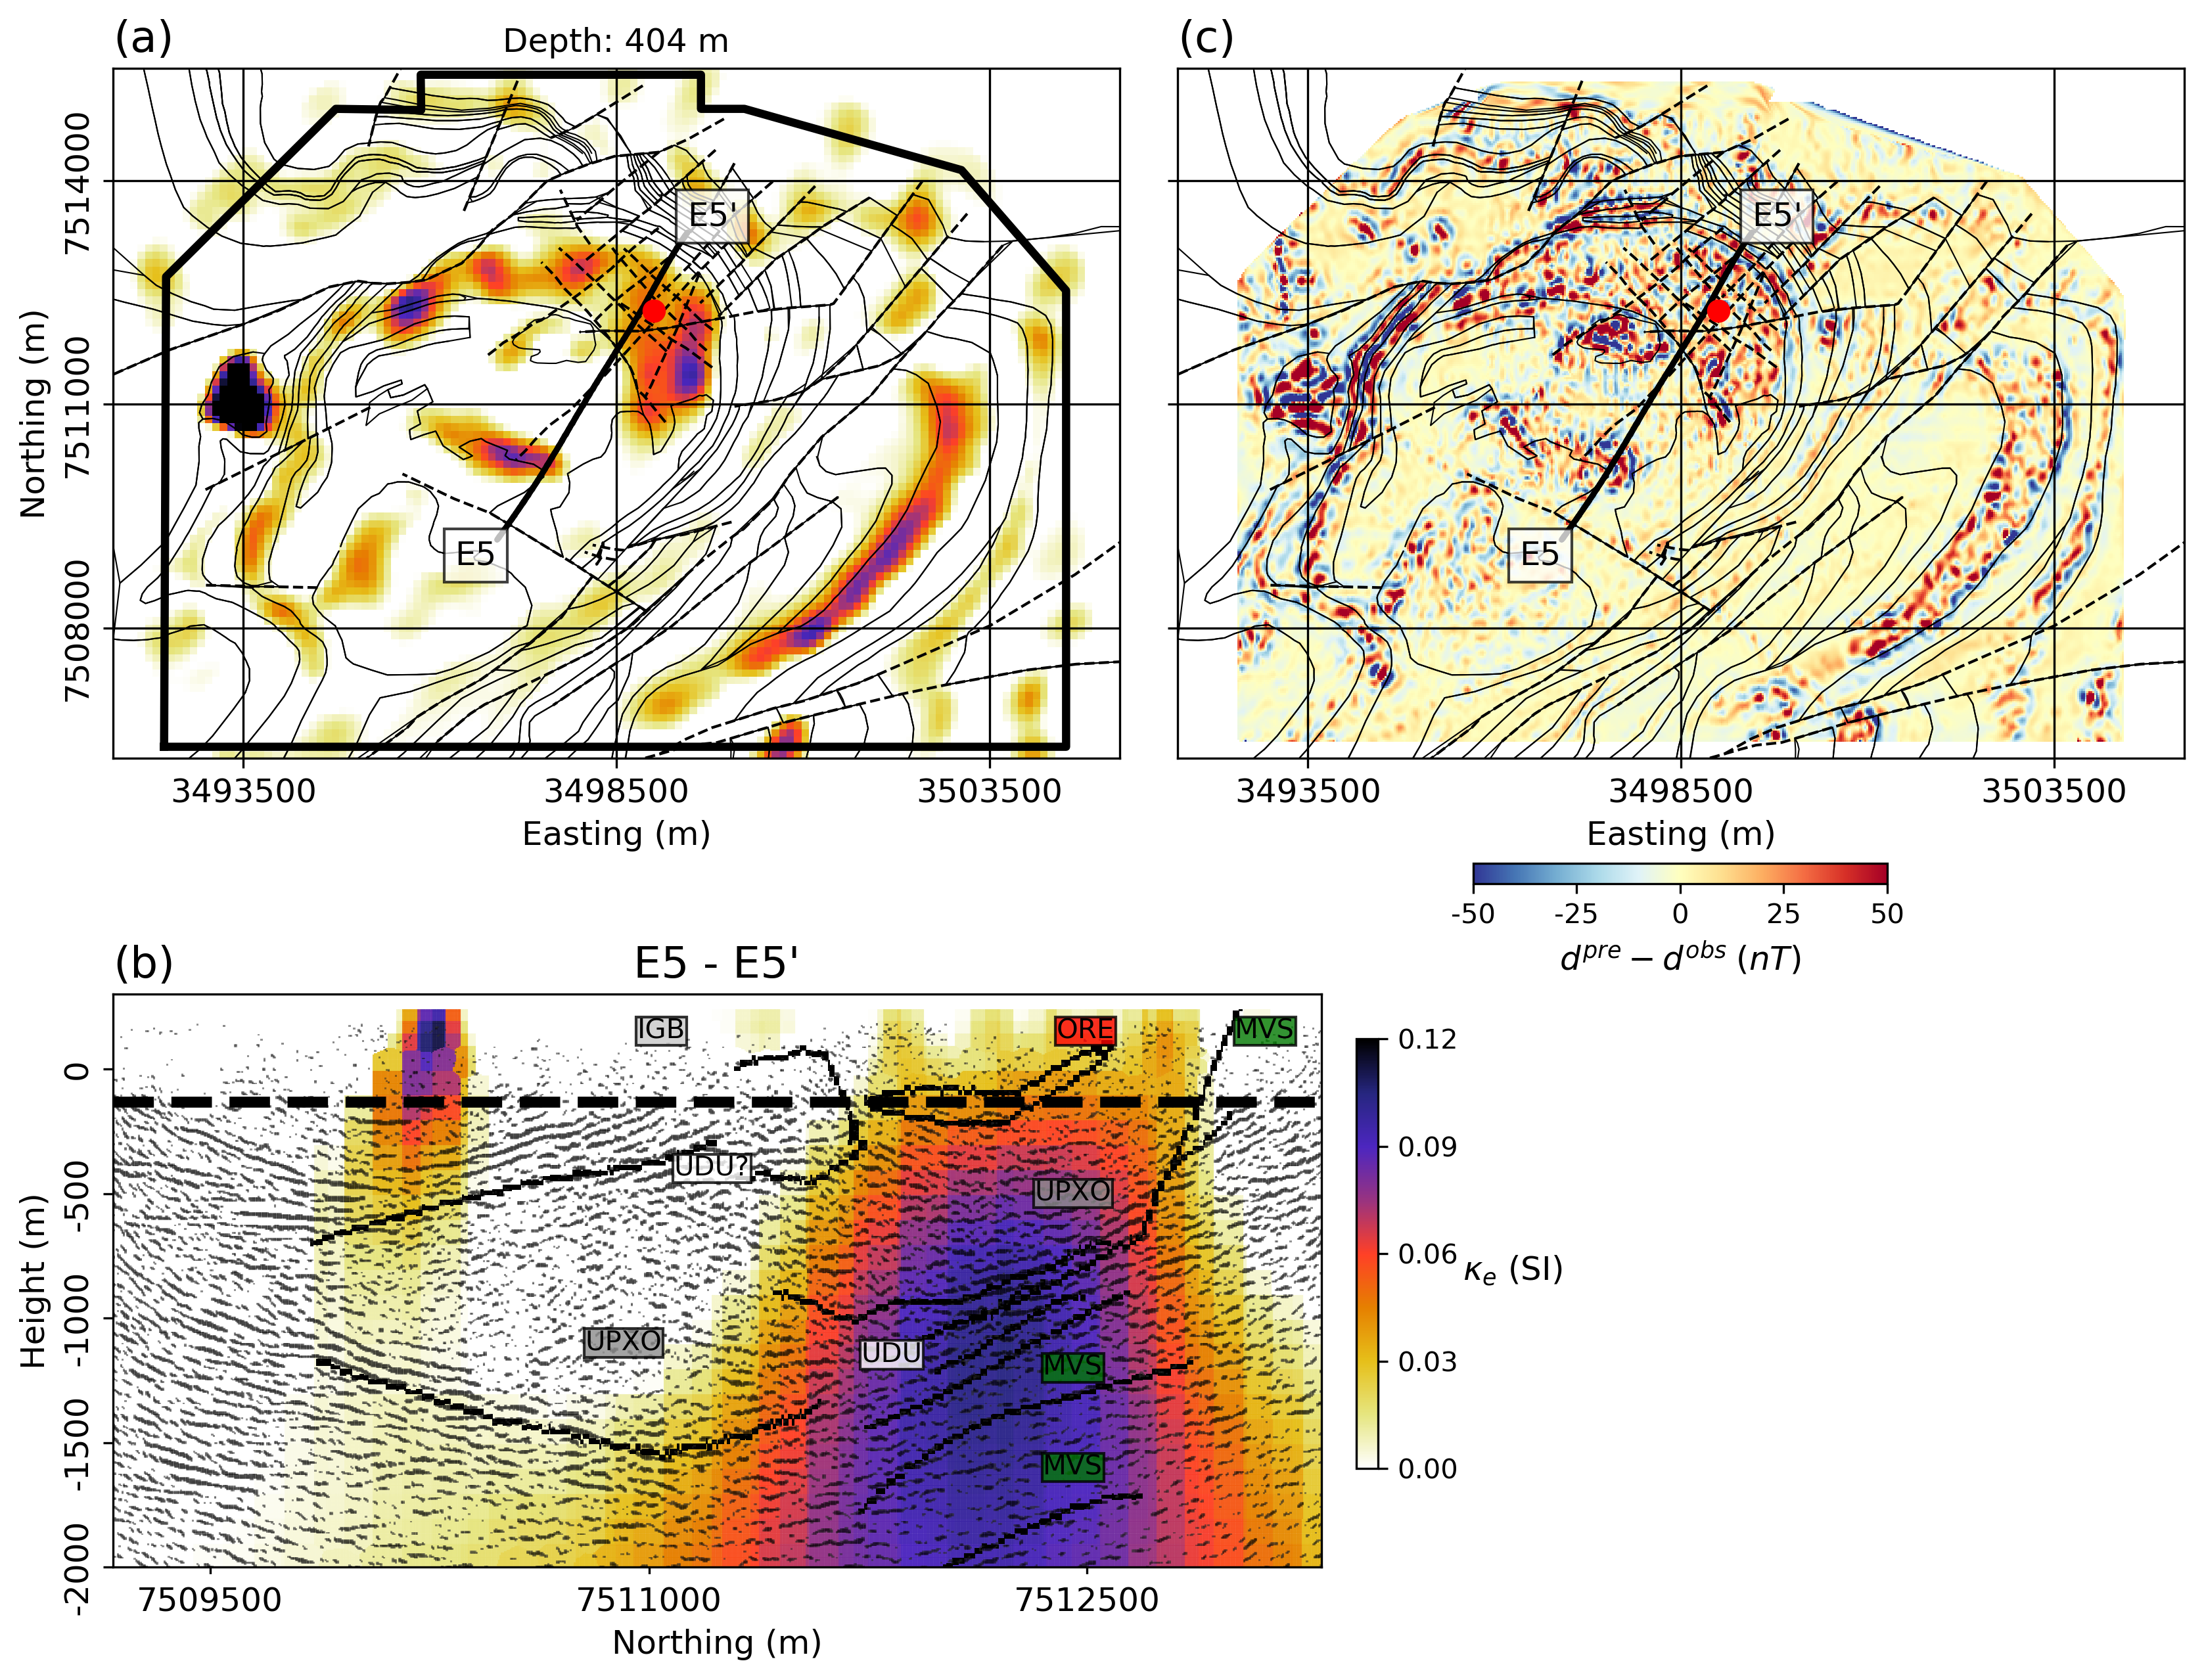
\includegraphics[width=\columnwidth]{Figures/Figure11.png}
\caption{(a) Horizontal and (b) vertical sections through the recovered susceptibility model that ignores the effect of remanence. Lithological contacts (black) identified by \cite{Koivisto2015} are shown for reference. (c) The residual map shows strong correlation with the negative magnetic data.}
\label{MAG_lp_EW}
\end{figure}

\begin{figure}[p!]
\includegraphics[width=\columnwidth]{Figures/Figure12.png}
\caption{Horizontal sections at $\approx$ 300 m below topography for a suite of models using various sparsity assumptions put on the amplitude of magnetization for $p_s\;, p_{x,y,z} \in [0,\: 2]$. Norm measure on the magnetization angle are fixed to $p_{x,y,z}=0$ in order to promote uniform magnetization direction.}
\label{MVIS_Hsections}
\end{figure}

\begin{figure}[p!]
\includegraphics[width=\columnwidth]{Figures/Figure13.png}
\caption{Vertical sections along the E5 seismic reflection line for a suite of models using various sparsity assumptions put on the amplitude of magnetization for $p_s\;, p_{x,y,z} \in [0,\: 2]$. Norm measure on the magnetization angle are fixed to $p_{x,y,z}=0$ in order to promote uniform magnetization direction.}
\label{MVIS_Vsections}
\end{figure}

\begin{figure}[p!]
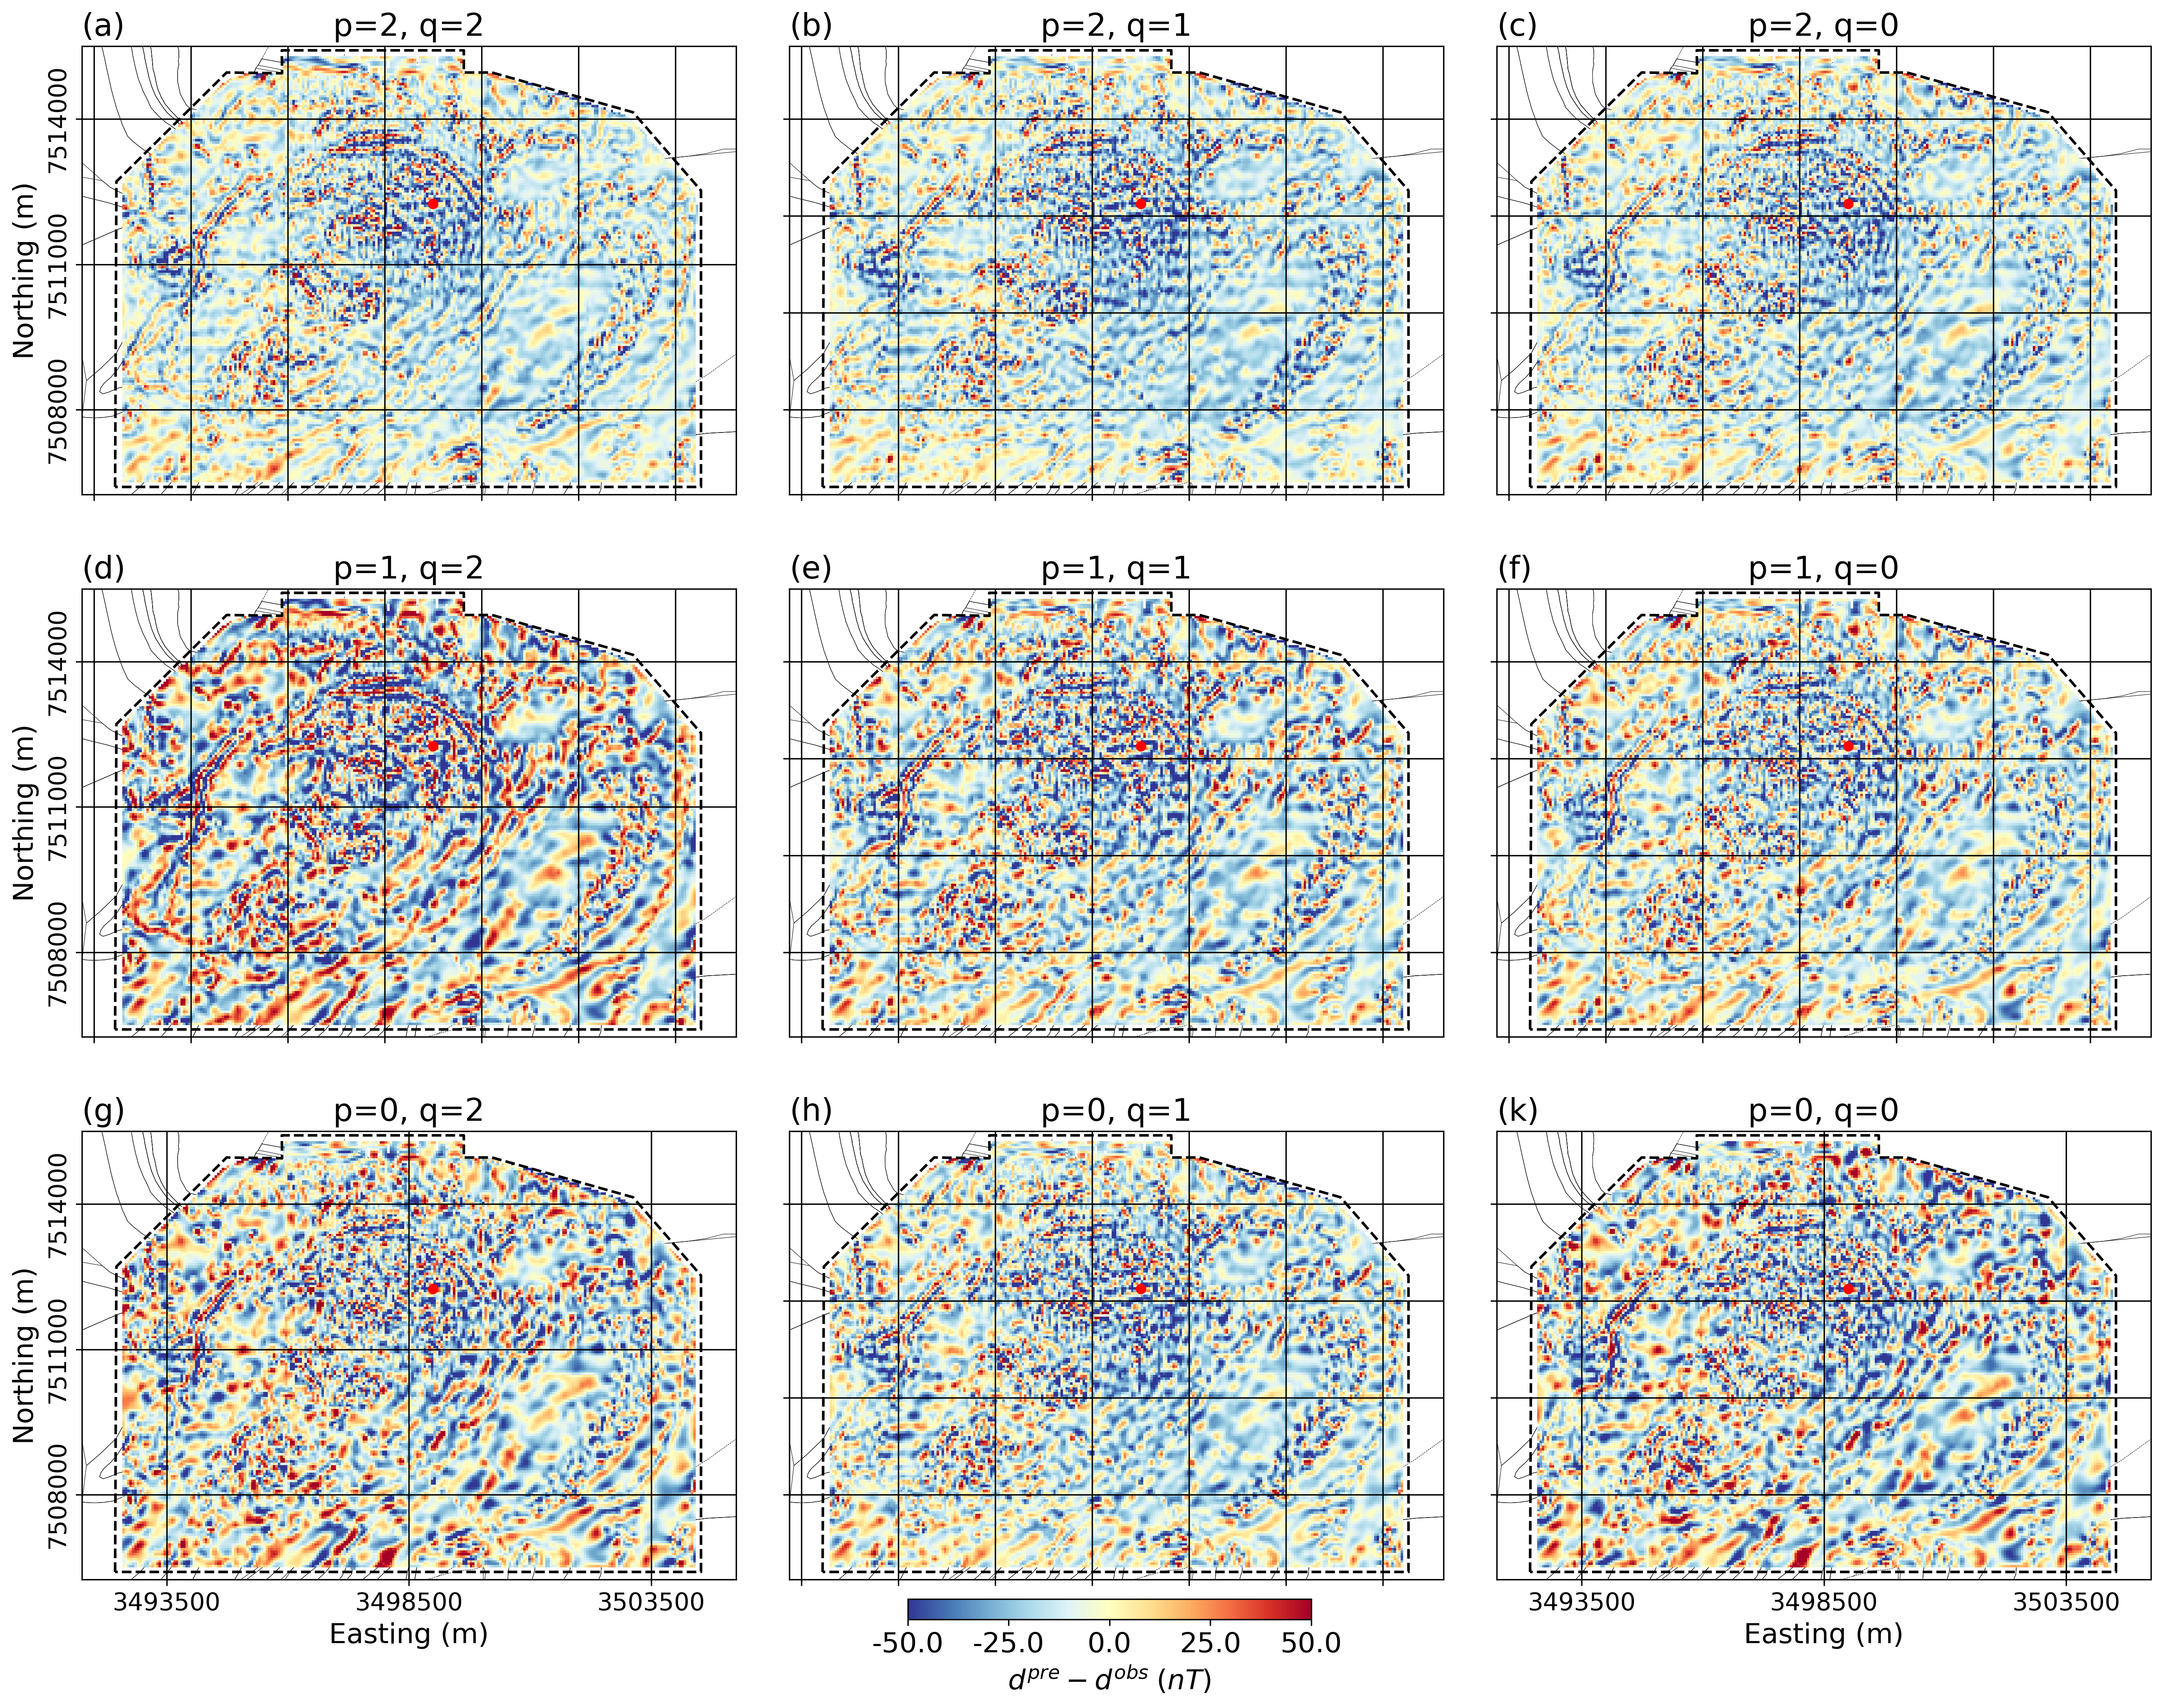
\includegraphics[width=\columnwidth]{Figures/Figure14.png}
\caption{Residual data maps for the nine inversions shown in Figure~\ref{MVIS_Hsections} and \ref{MVIS_Vsections}.}
\label{MVIS_predicted}
\end{figure}

\begin{figure}[p!]
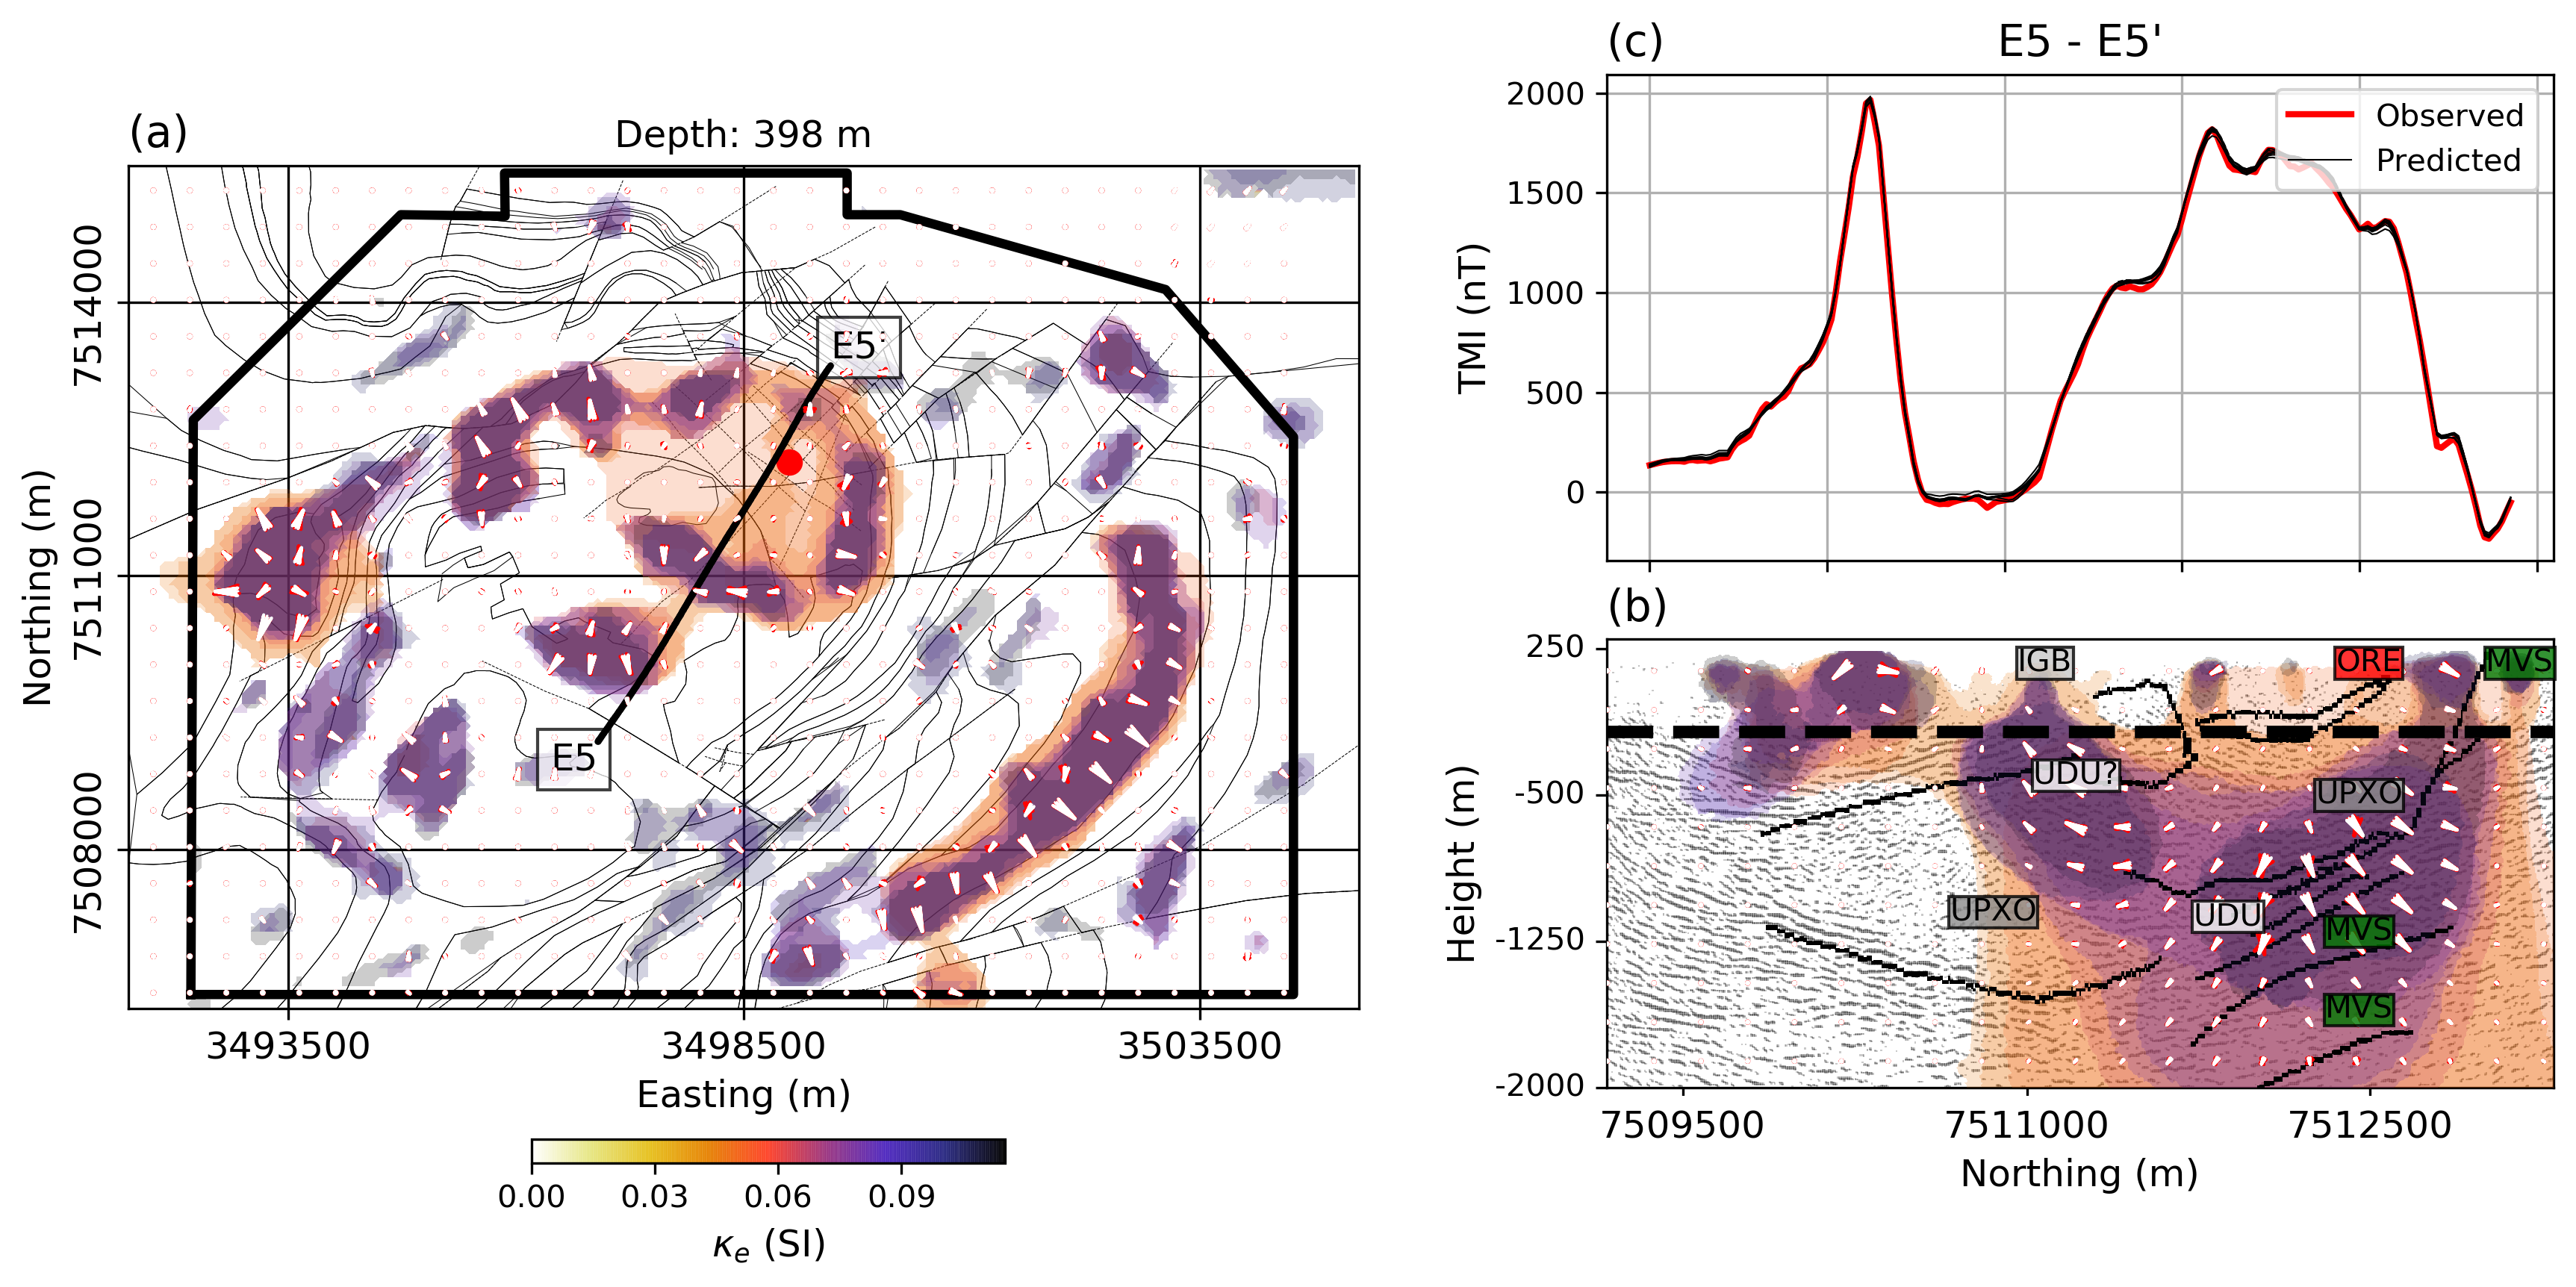
\includegraphics[width=\columnwidth]{Figures/Figure15.png}
\caption{(a) Horizontal and (b) vertical sections through iso-contours of magnetization recovered from nine mixed $\ell_p$-norm inversions. Magnetization orientation (white arrowheads) and standard deviation on the angle (red arrowheads) are shown. (c) Data profile along the E5 section for the observed and predicted data calculated from the recovered models.}
\label{MVIS_Iso_model}
\end{figure}

\end{document}



\bibliography{references}
\bibliographystyle{seg}

%\listoffigures
\pagebreak
%\listoftables

\begin{table}
\caption{Intervals along boreholes KV200 and KV297 reporting significant remanent magnetization.}
\label{Table1}
\end{table}

\begin{table}
\caption{Summary table grouping the various lithological units logged from boreholes. Expected magnetic susceptibility contrasts are derived from Figure~\ref{Kevitsa_PhysProp}.}
\label{Table2}
\end{table}

\pagebreak

\begin{figure}[p!]
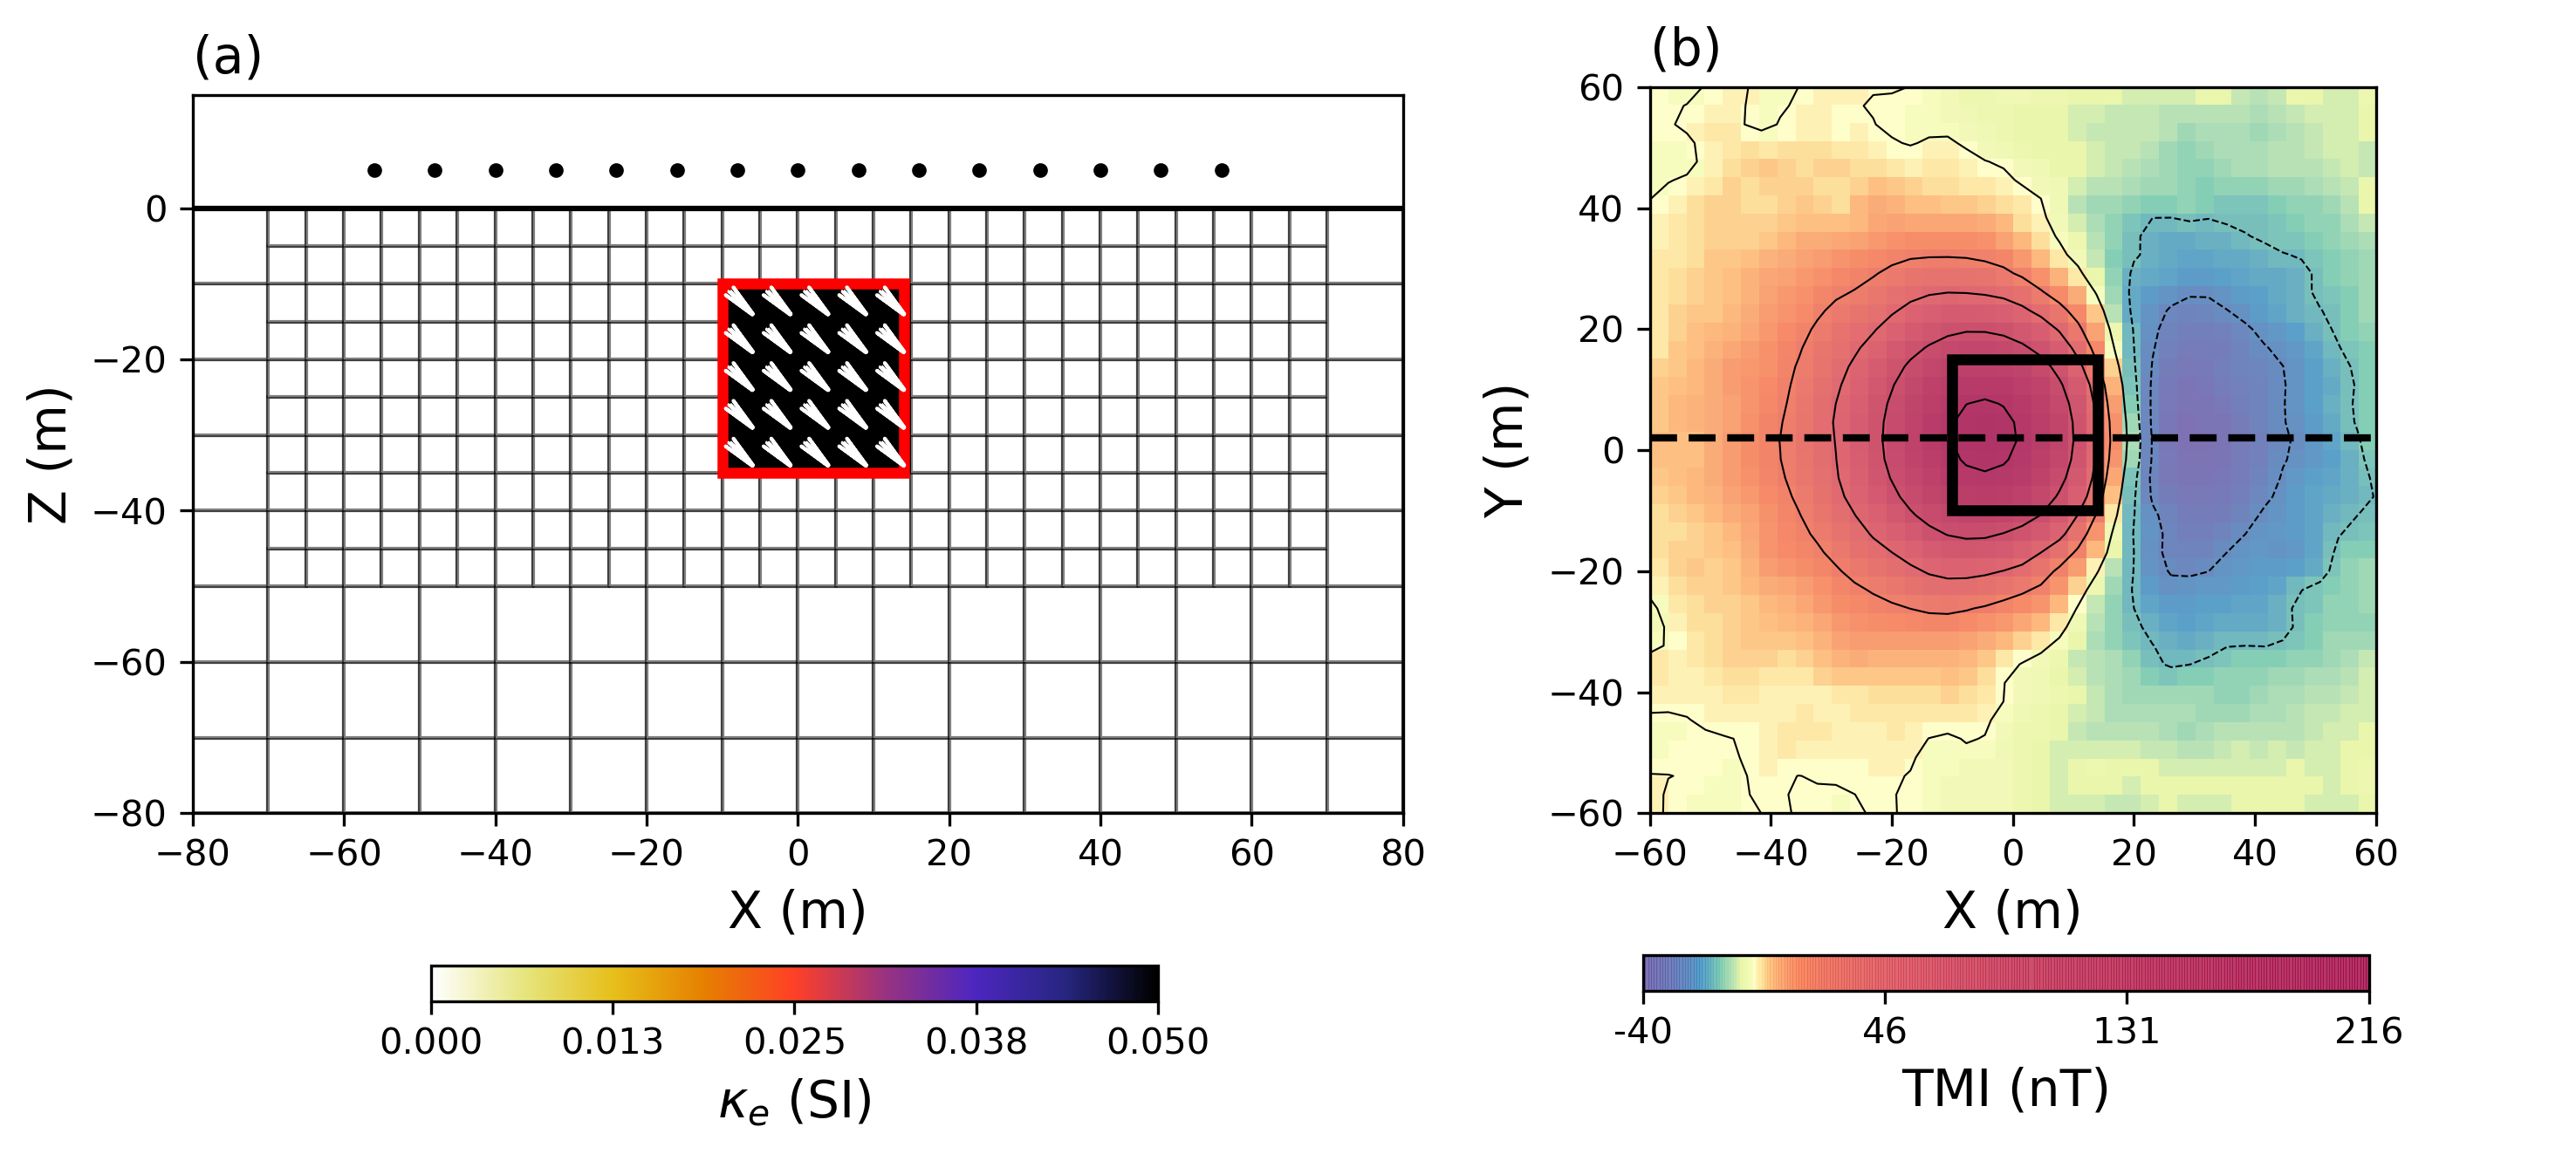
\includegraphics[width=\columnwidth]{Figures/Figure1.png}
\caption{(a) Vertical section through the synthetic block model (Y = 0 m) with magnetization $\mathbf{M}$ [$2.0\: A/m,\; I: 45^\circ,\; D: 90^\circ$]($\kappa_e$ = 0.05 SI). Survey points (black dots) are placed 15 m above the magnetic anomaly. (b) Simulated TMI data map with random Gaussian noise added, 1 nT standard deviation. The horizontal position of the block is shown in black for reference.}
\label{REM_model}
\end{figure}

\begin{figure}[p!]
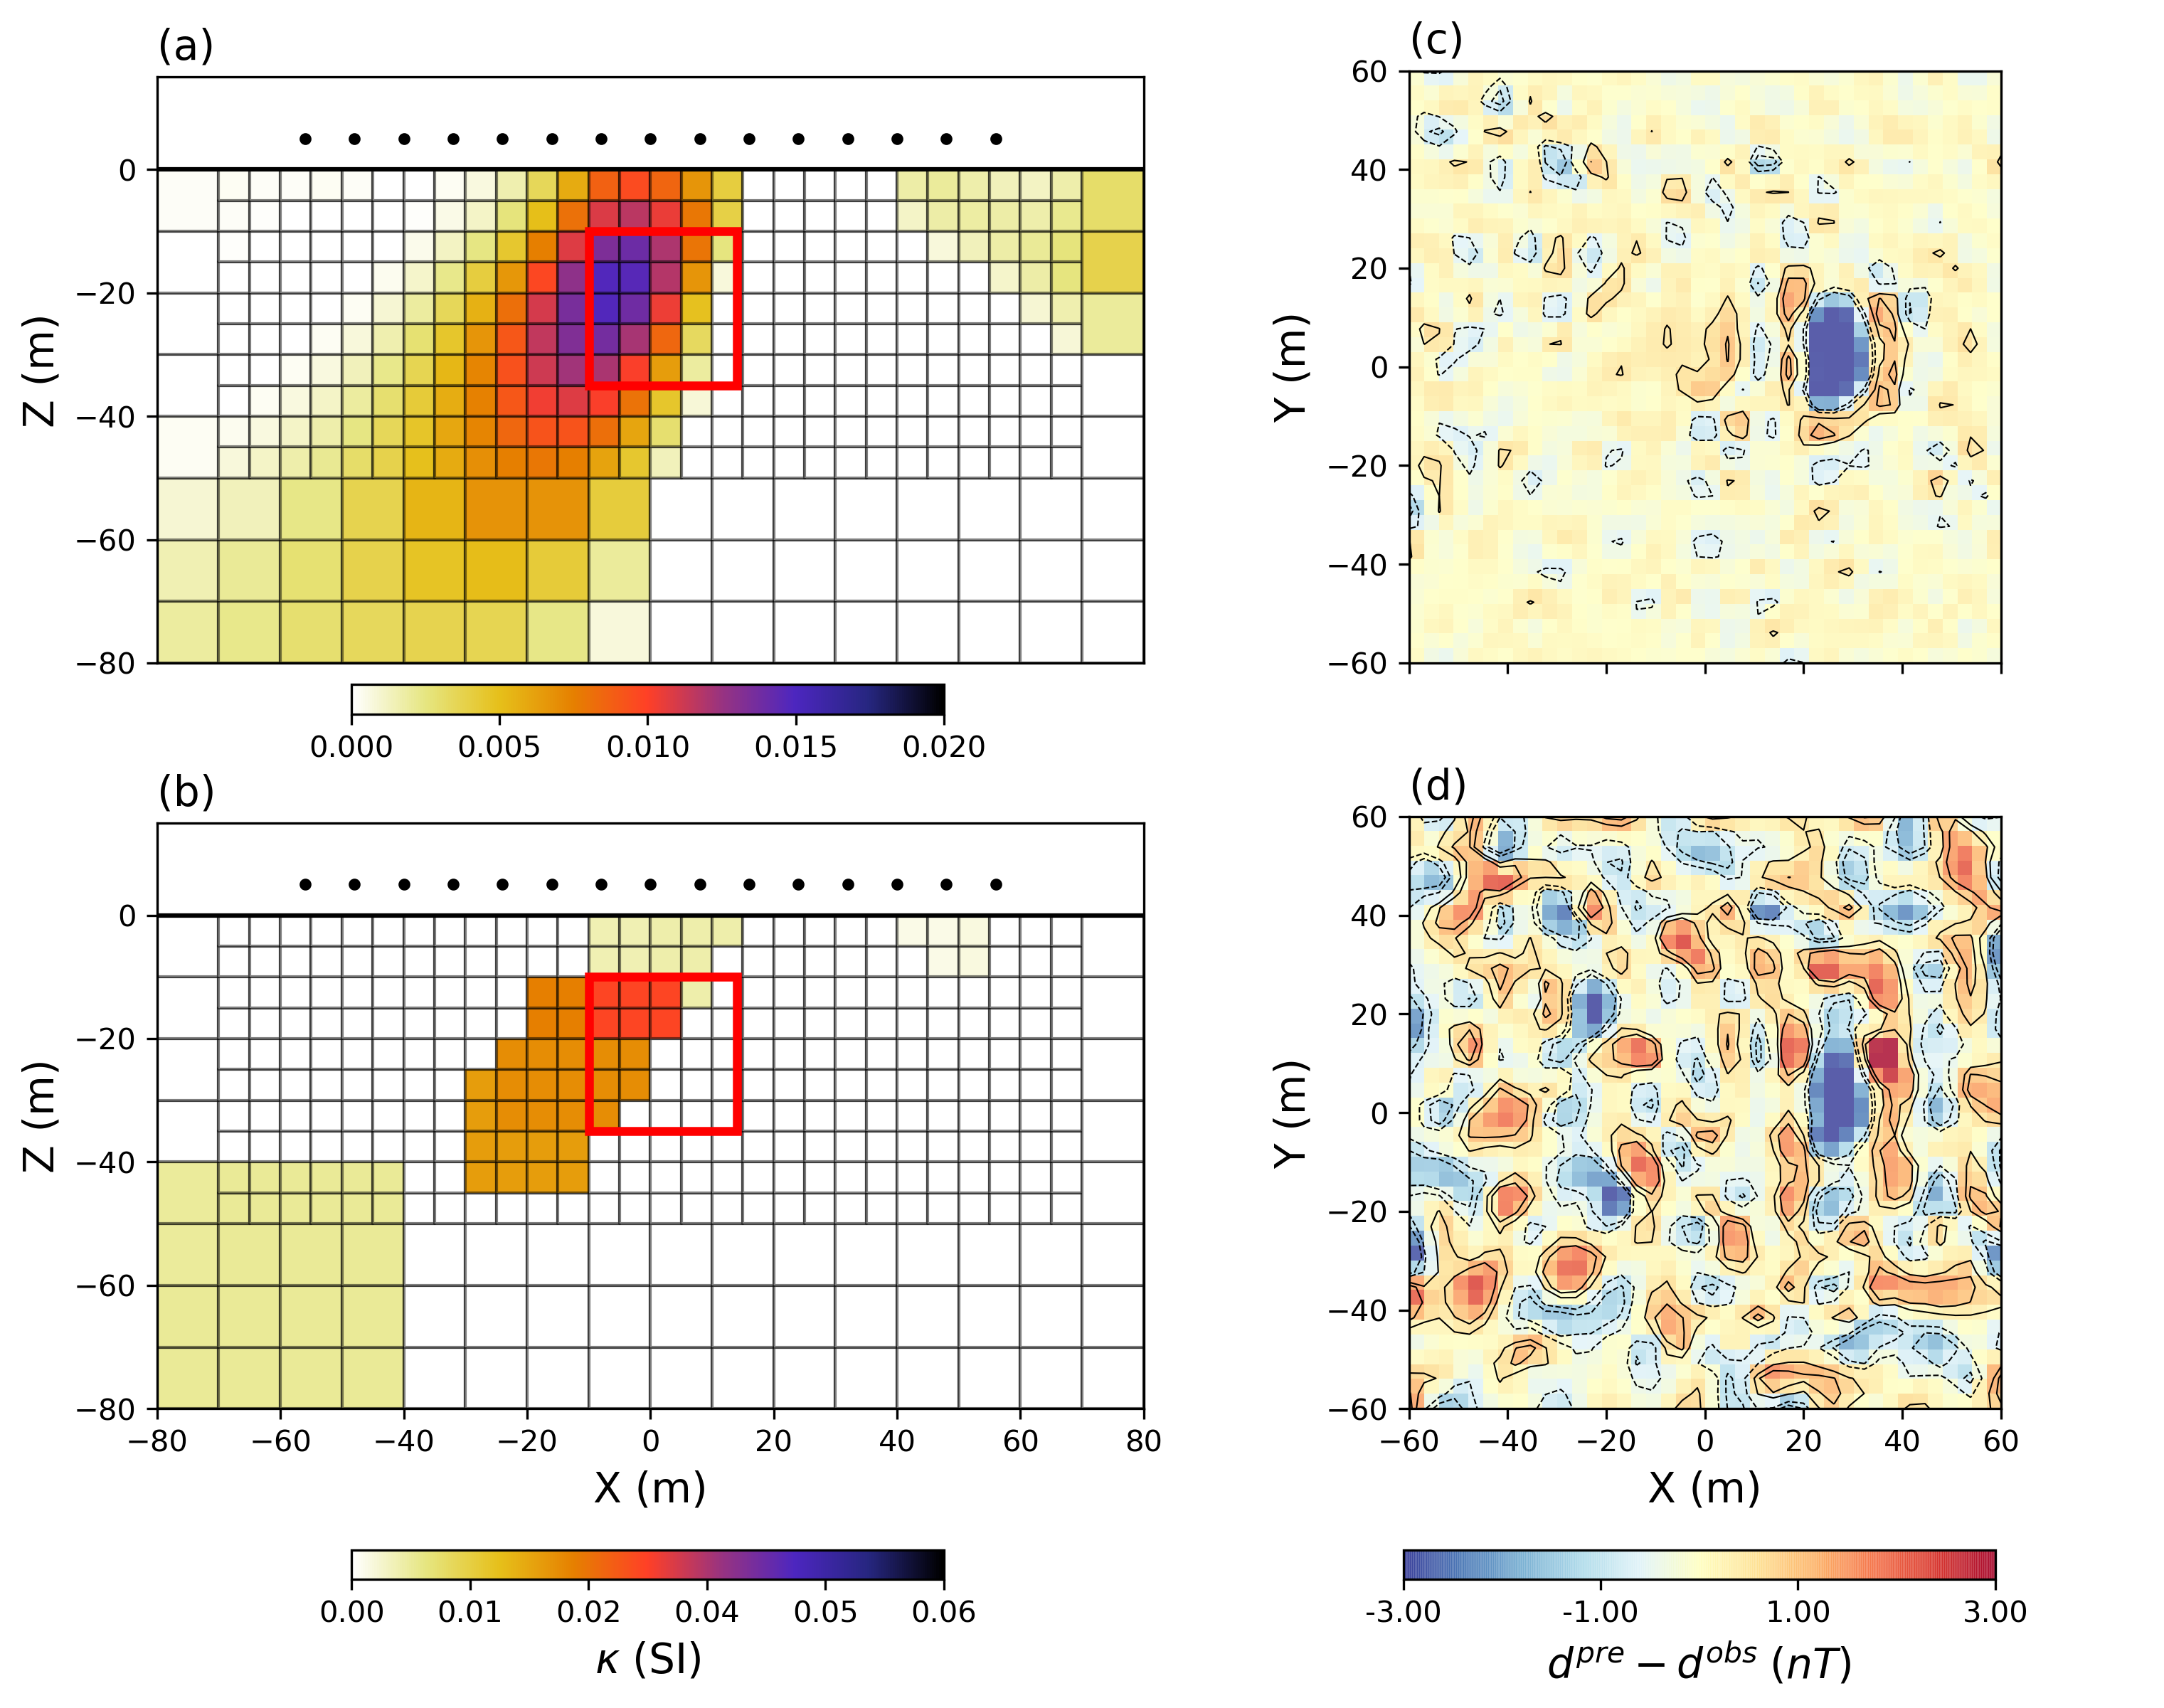
\includegraphics[width=\columnwidth]{Figures/Figure2.png}
\caption{Vertical section through the recovered susceptibility model using (a) smooth assumption ($p_s, \;p_x,\; p_y,\; p_z = 2$) and (b) sparse $\ell_p$-norms to recover a compact model ($p_s,\;p_x,\; p_y,\; p_z = 0$). Both solutions show an anomaly with a false dip due to the wrong assumption of a vertical magnetization. Data residuals for (c) the smooth and (d) compact solution shows correlated signal with the negative data.}\label{Susc_model}
\end{figure}

\begin{figure}[p!]
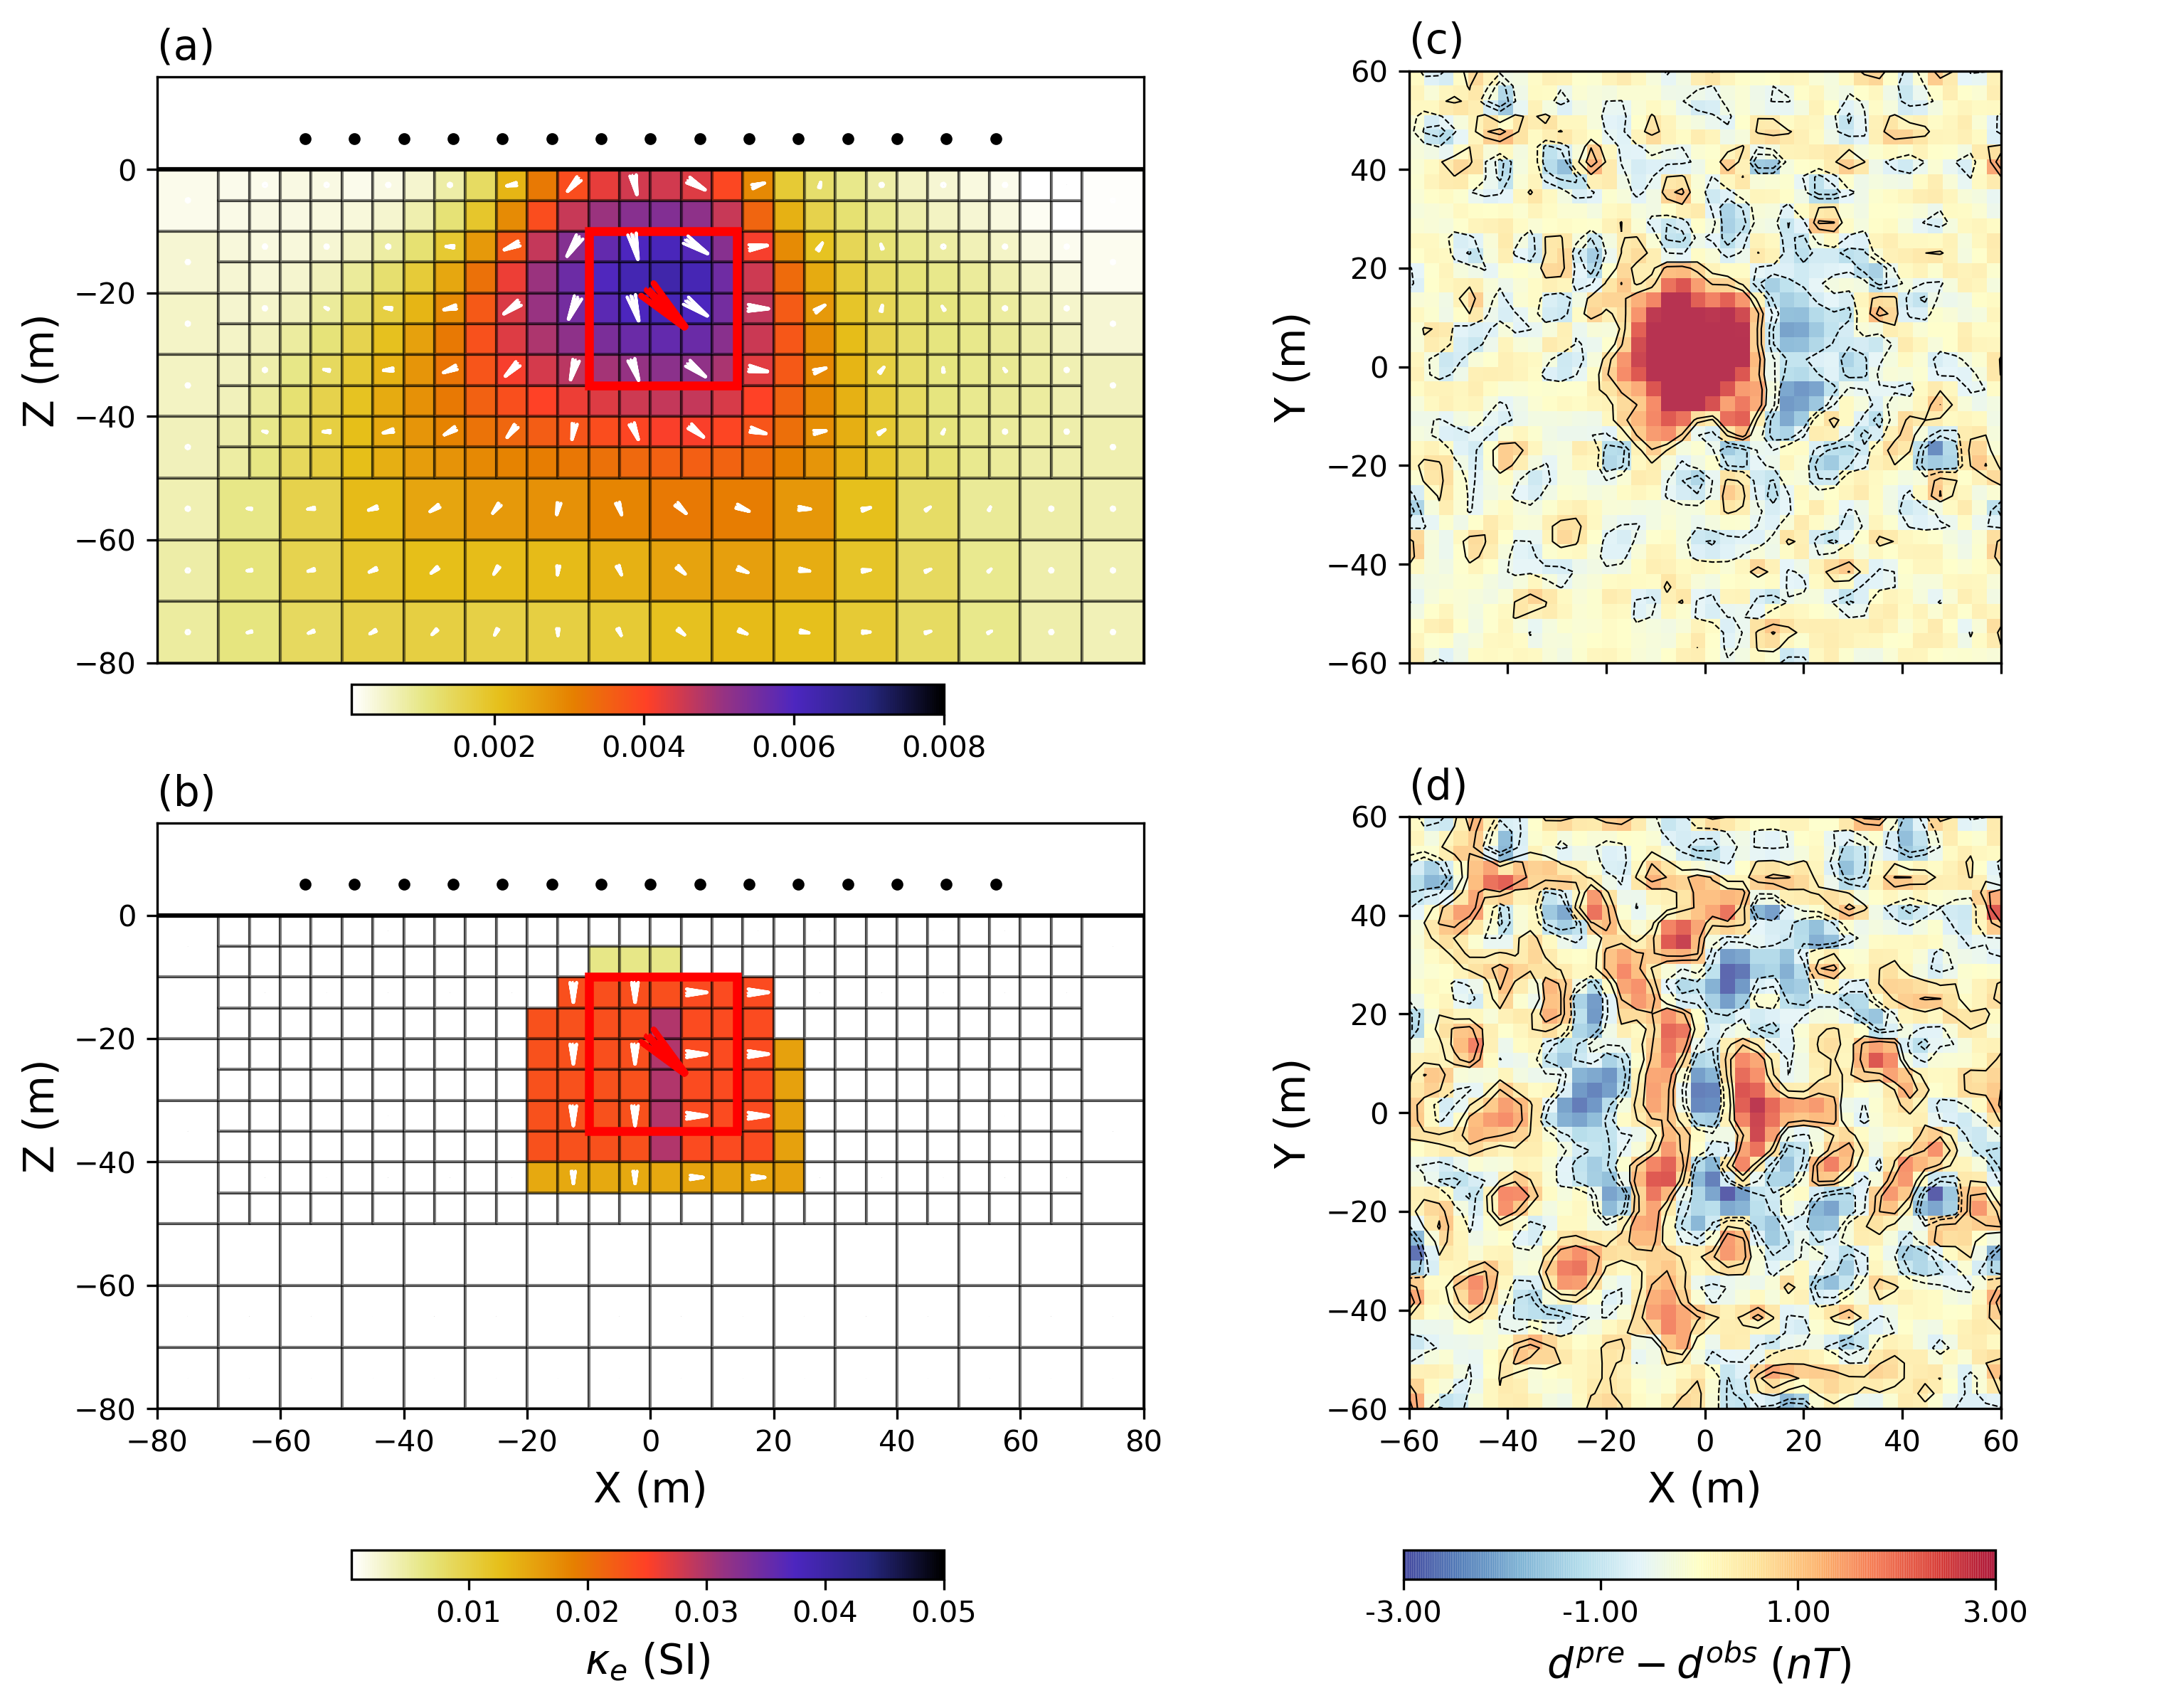
\includegraphics[width=\columnwidth]{Figures/Figure3.png}
\caption{Vertical section through the recovered magnetization vector model using the Cartesian formulation with (a) smooth $l_2$-norm assumption and (b) sparsity constraints applied on all three Cartesian components ($p_{i_s}, \;p_{i_x},\; p_{i_y},\; p_{i_z} = 0$). Color is scaled by the magnitude of magnetization. The true magnetization direction is shown with a red arrow. Data residual map calculated with (c) the smooth and (d) compact solution.}
\label{MVI_C_model}
\end{figure}

\begin{figure}[p!]
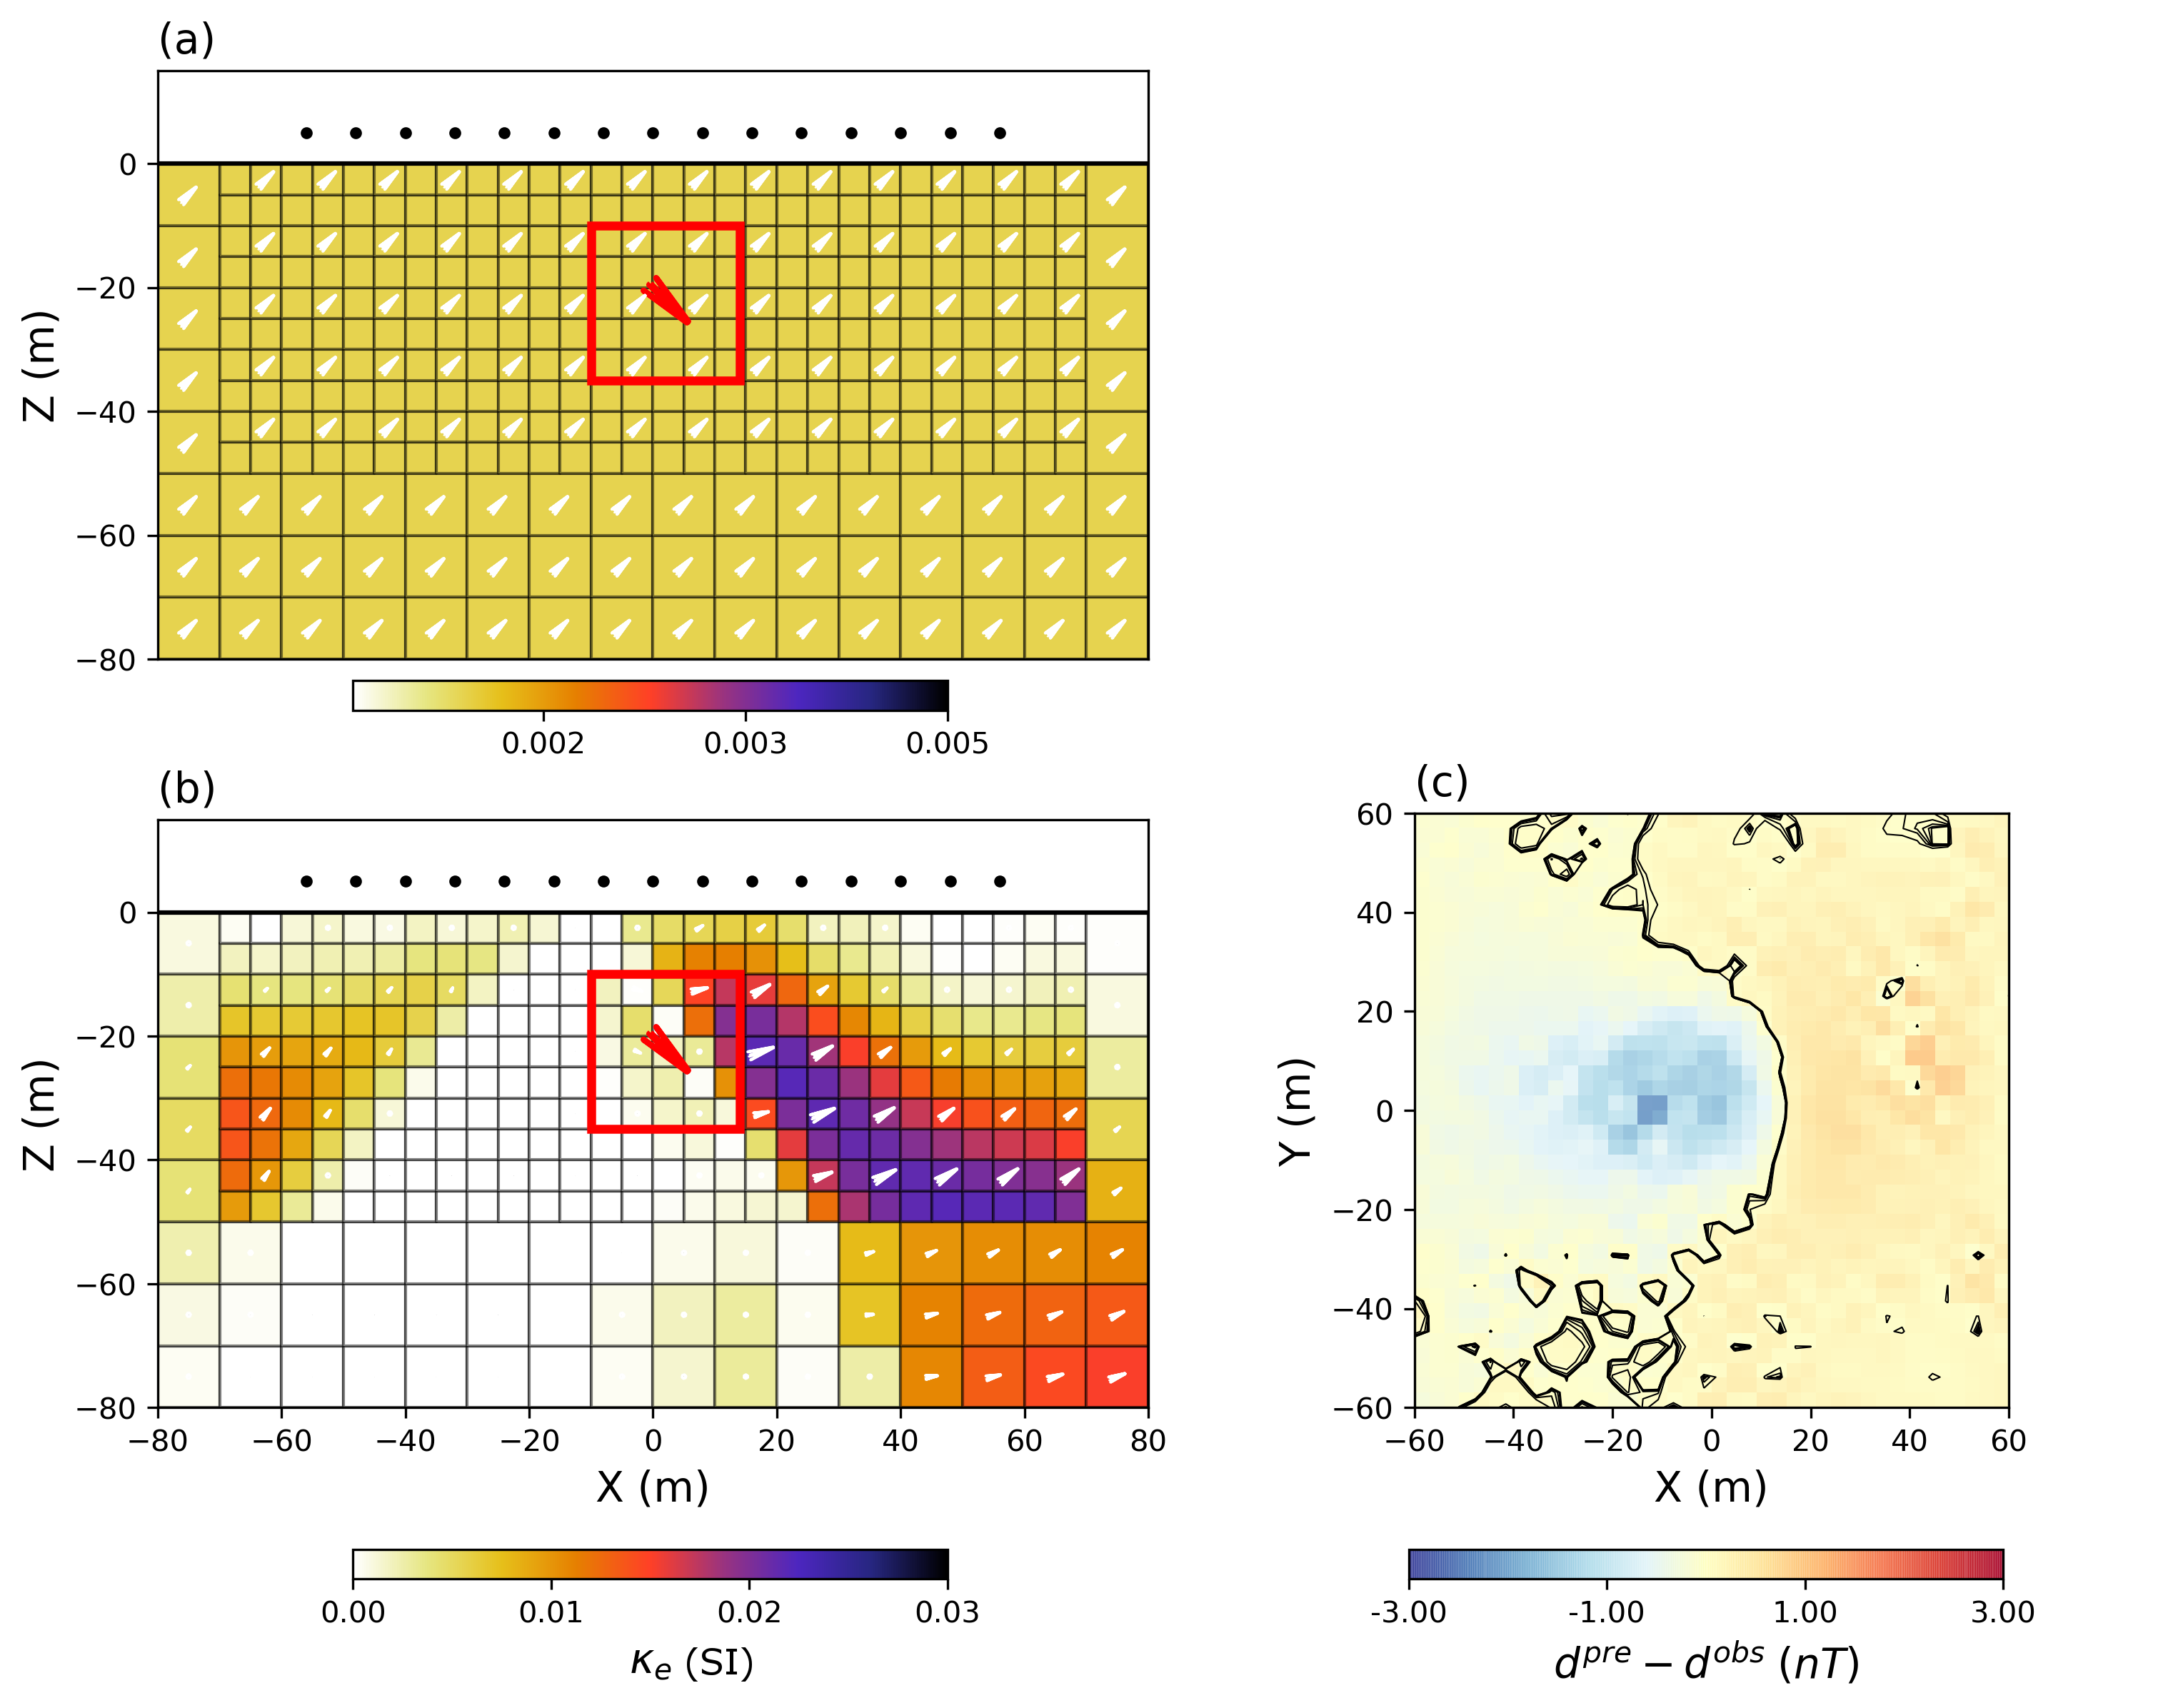
\includegraphics[width=\columnwidth]{Figures/Figure4.png}
\caption{ Vertical section through the (a) starting model and (b) recovered magnetization vector model in spherical coordinates with its (c) data residual map. The inversion stopped after three iterations, unable to further reduce the objective function.}
\label{MVI_S_model_noScale}
\end{figure}

\begin{figure}[p!]
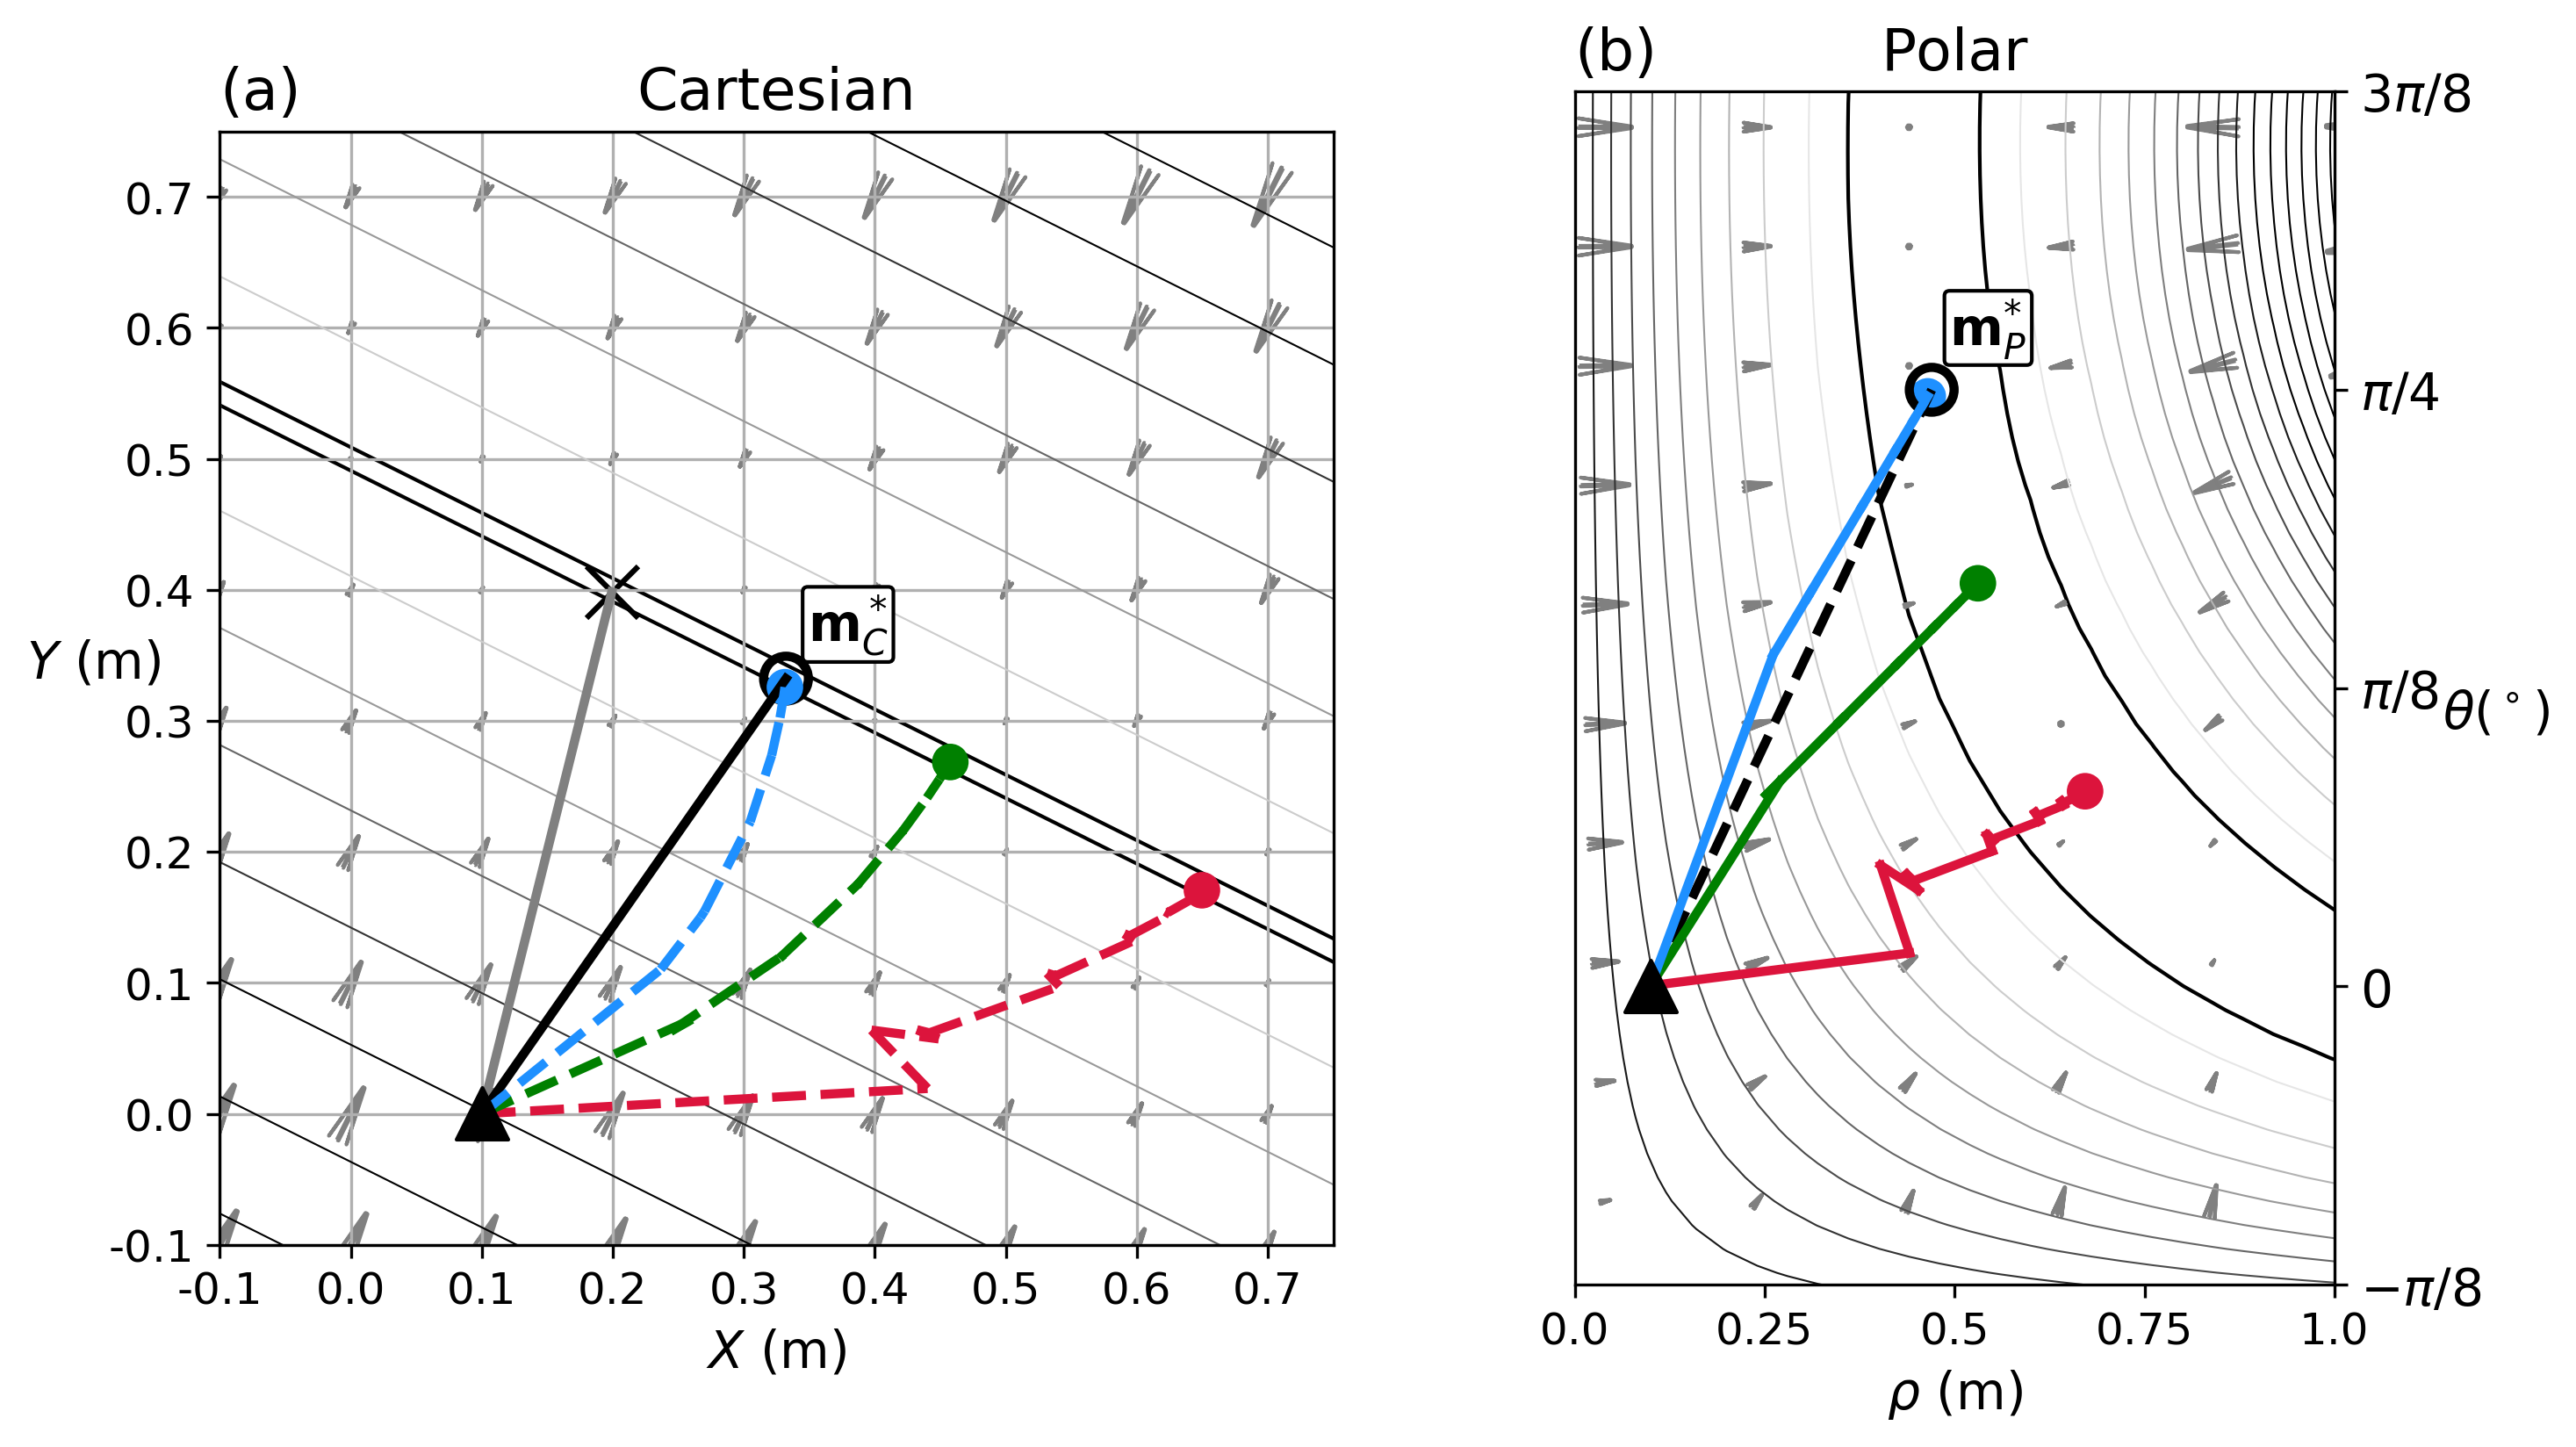
\includegraphics[width=\columnwidth]{Figures/Figure5.png}
\caption{Contour maps for the objective functions of a two-parameter inverse problem solved in (a) Cartesian and (b) polar coordinate systems. Solid colored lines show the model updates taken by different algorithms in their respective coordinate systems and, in dash, the equivalent steps in the other domain for comparison. Each inversion started with the same initial model (triangle). The colors and inversions are: Gray: the non-weighted Cartesian problem; Black: the sensitivity weighted Cartesian problem; Red: the non-linear polar coordinate system with fixed sensitivity weights; Green: the polar problem with iterative sensitivity re-weighting; and Blue: with the added scaling to compensate for the dynamic range of the parameters (see equation~50). }
\label{NonLinearGN}
\end{figure}

\begin{figure}[p!]
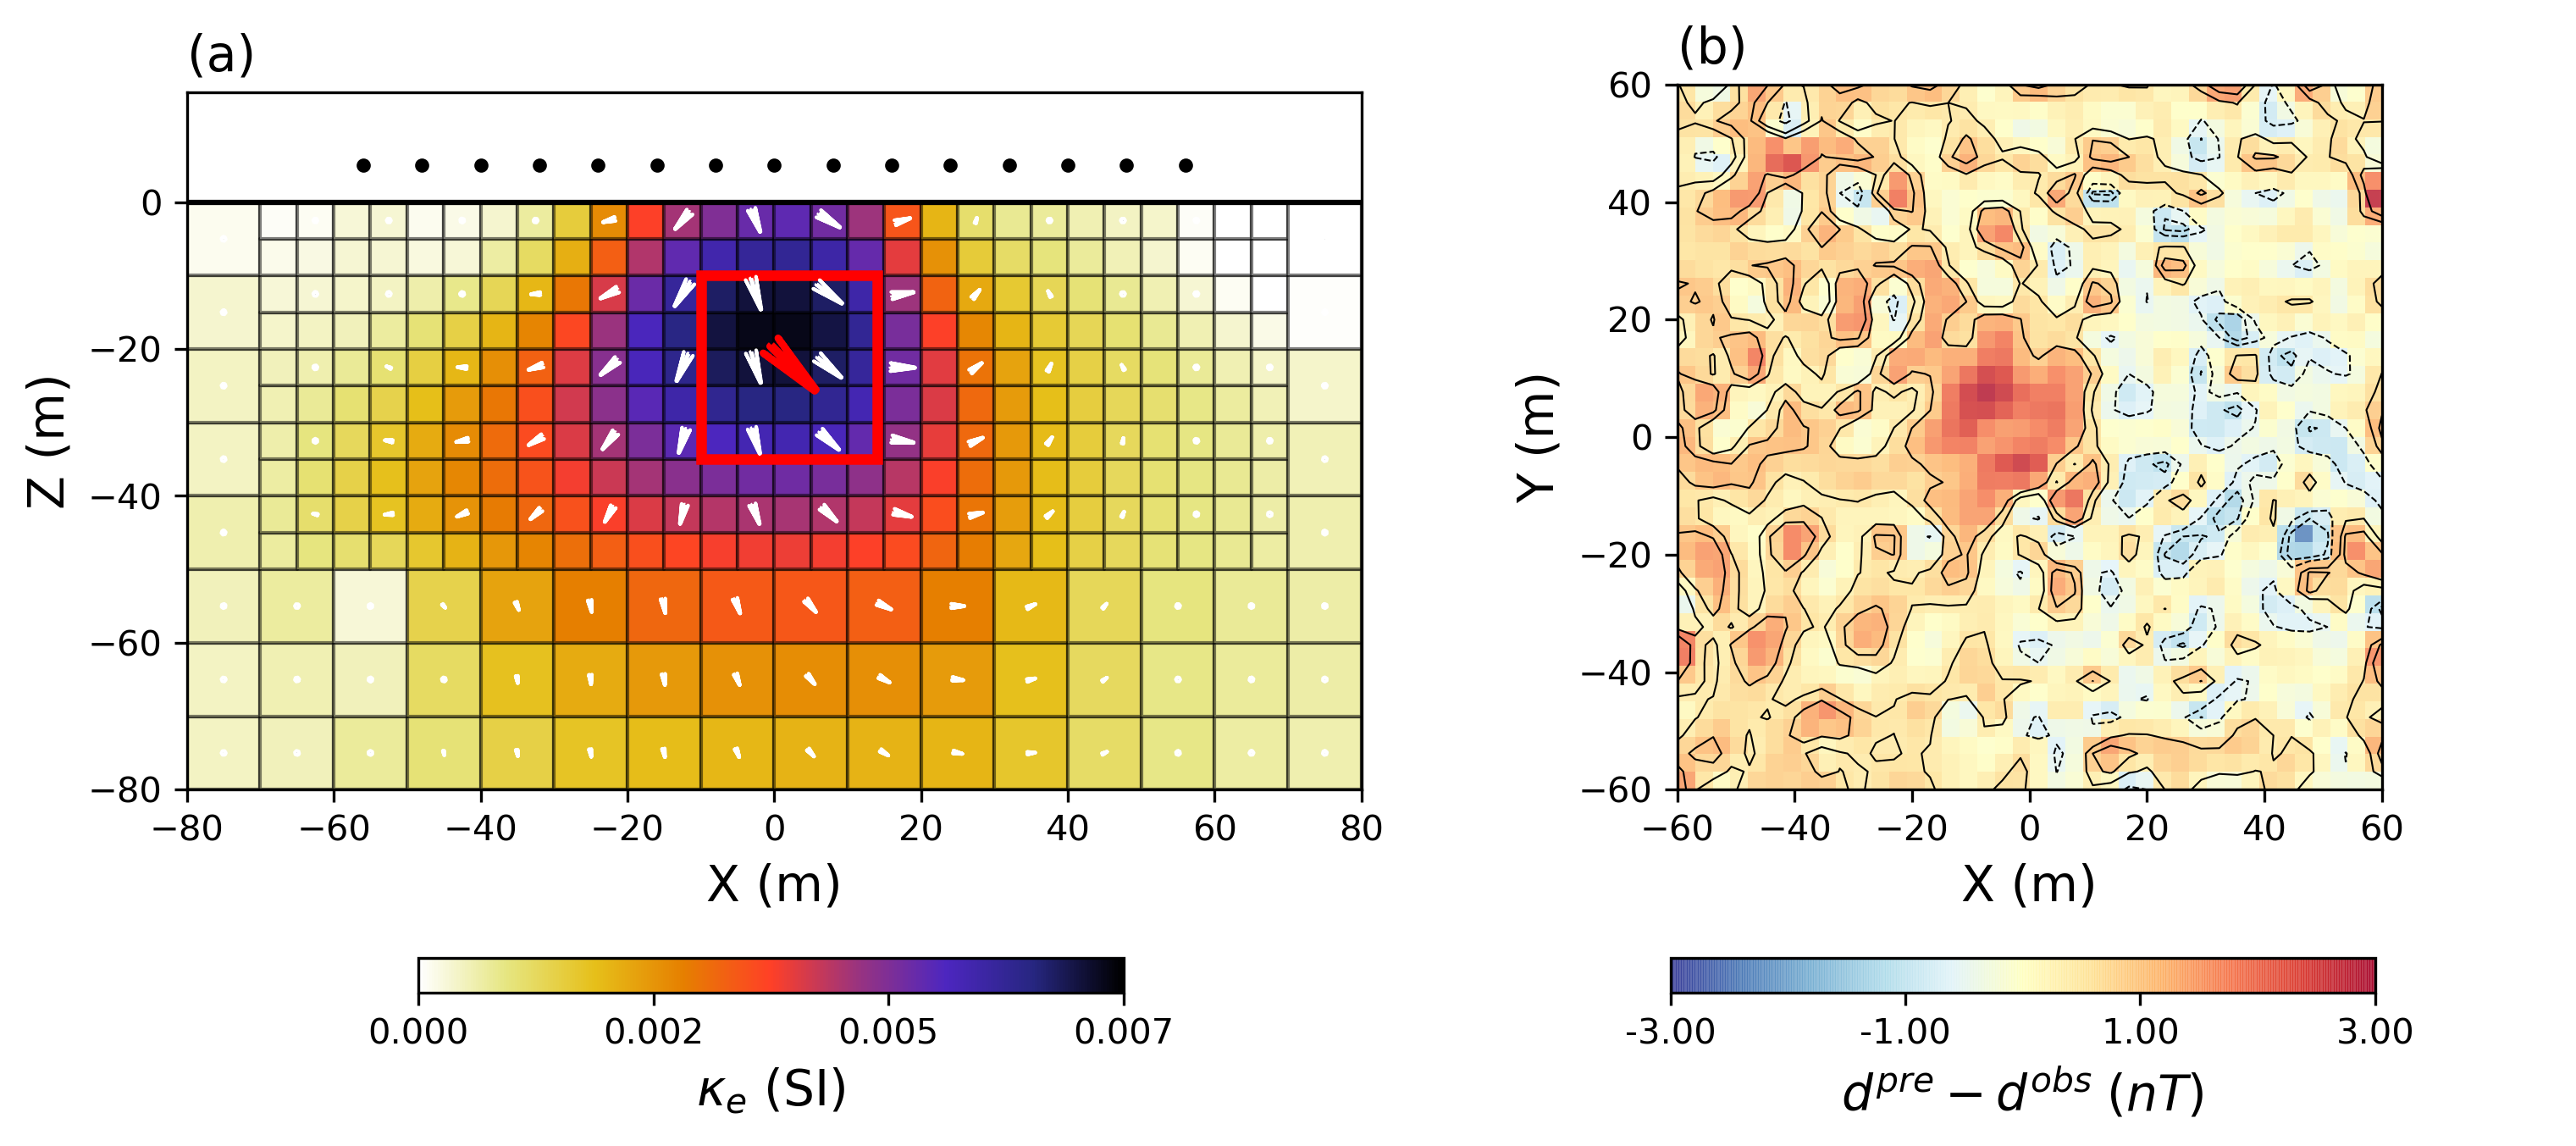
\includegraphics[width=\columnwidth]{Figures/Figure6.png}
\caption{(a) Vertical section through the recovered magnetization vector model in spherical coordinates using sensitivity based weighting and (b) the corresponding data residual map. The same poor starting model shown in Figure~\ref{MVI_S_model_noScale}a was used, but the algorithm converged to a solution similar to the Cartesian solution.}
\label{MVI_S_model}
\end{figure}

\begin{figure}[p!]
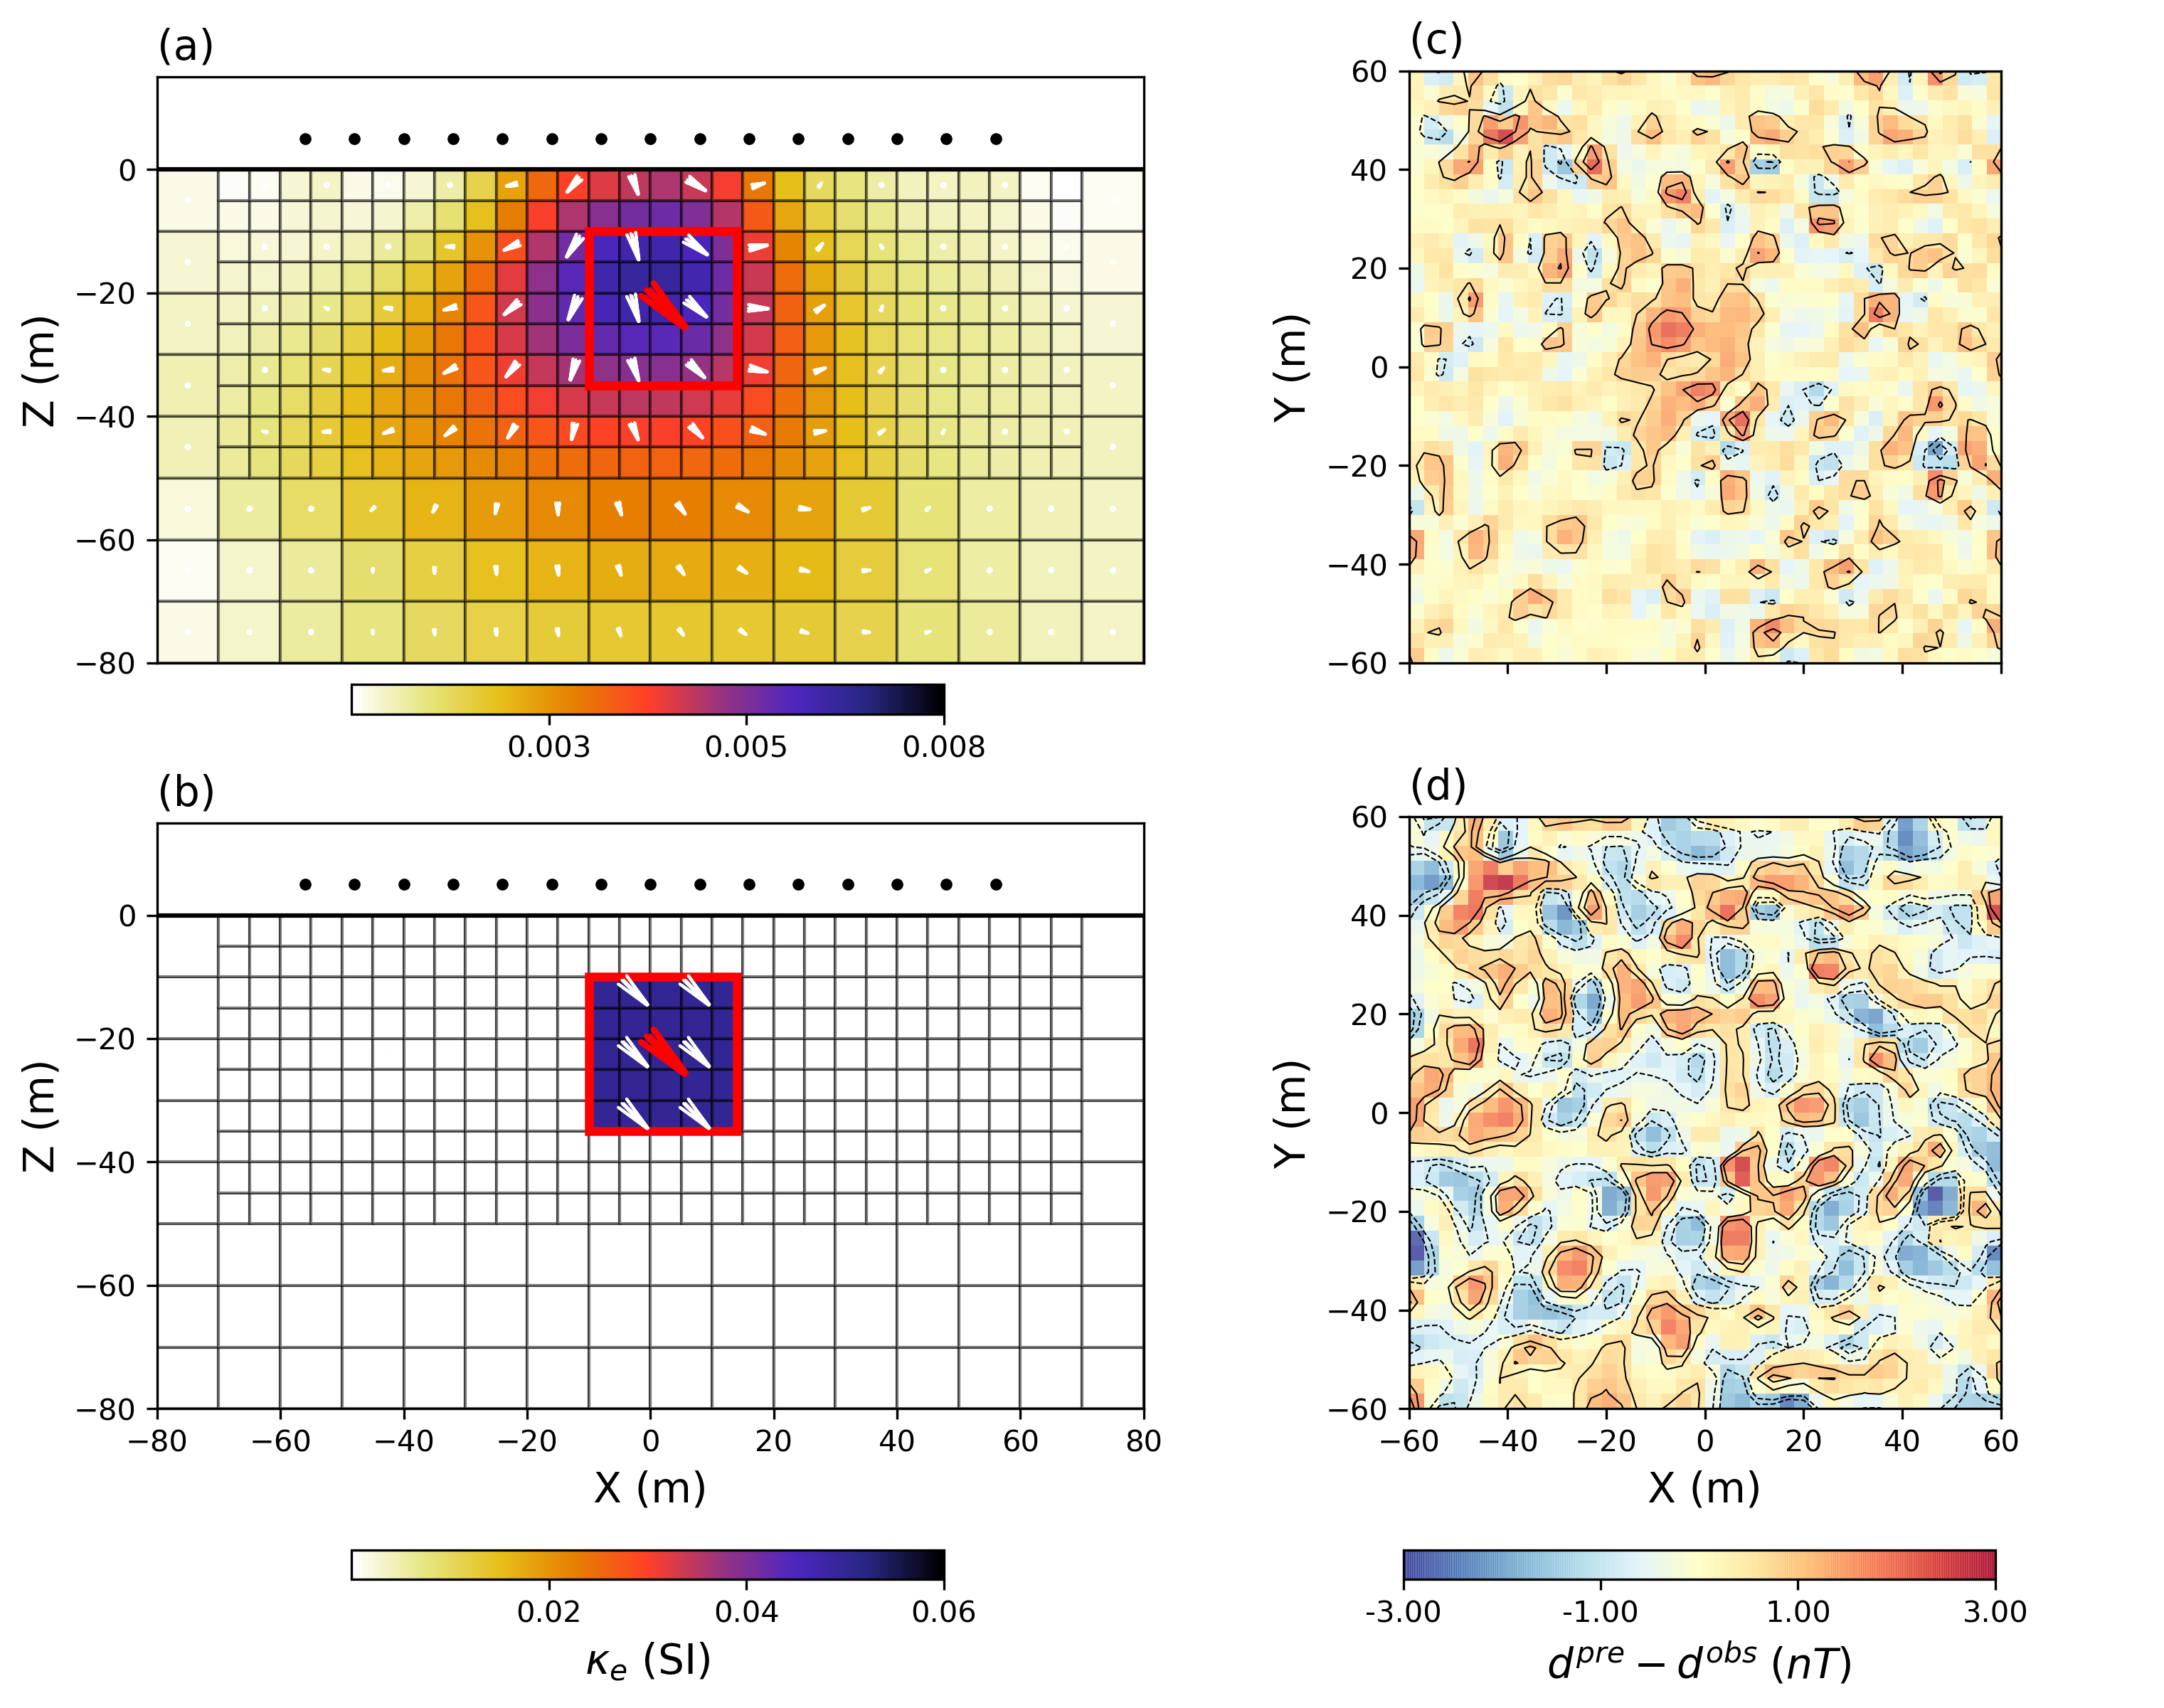
\includegraphics[width=\columnwidth]{Figures/Figure7.png}
\caption{Vertical section through the recovered magnetization vector model in spherical coordinates using sensitivity based weighting and the smooth Cartesian solution as starting model: (a) smooth regularization ($p_s=p_x=p_y=p_z = 2$) and (b) sparse norms on the strength and angles of the magnetization vector ($p_s=p_x=p_y=p_z = 0$). By using the sparse norms, we recover a solution that closely resembles the true model and, as observed in (d), we also eliminate the coherent signal in the residual data that is observed in (c).}
\label{MVI_S_model_lp}
\end{figure}

\begin{figure}[p!]
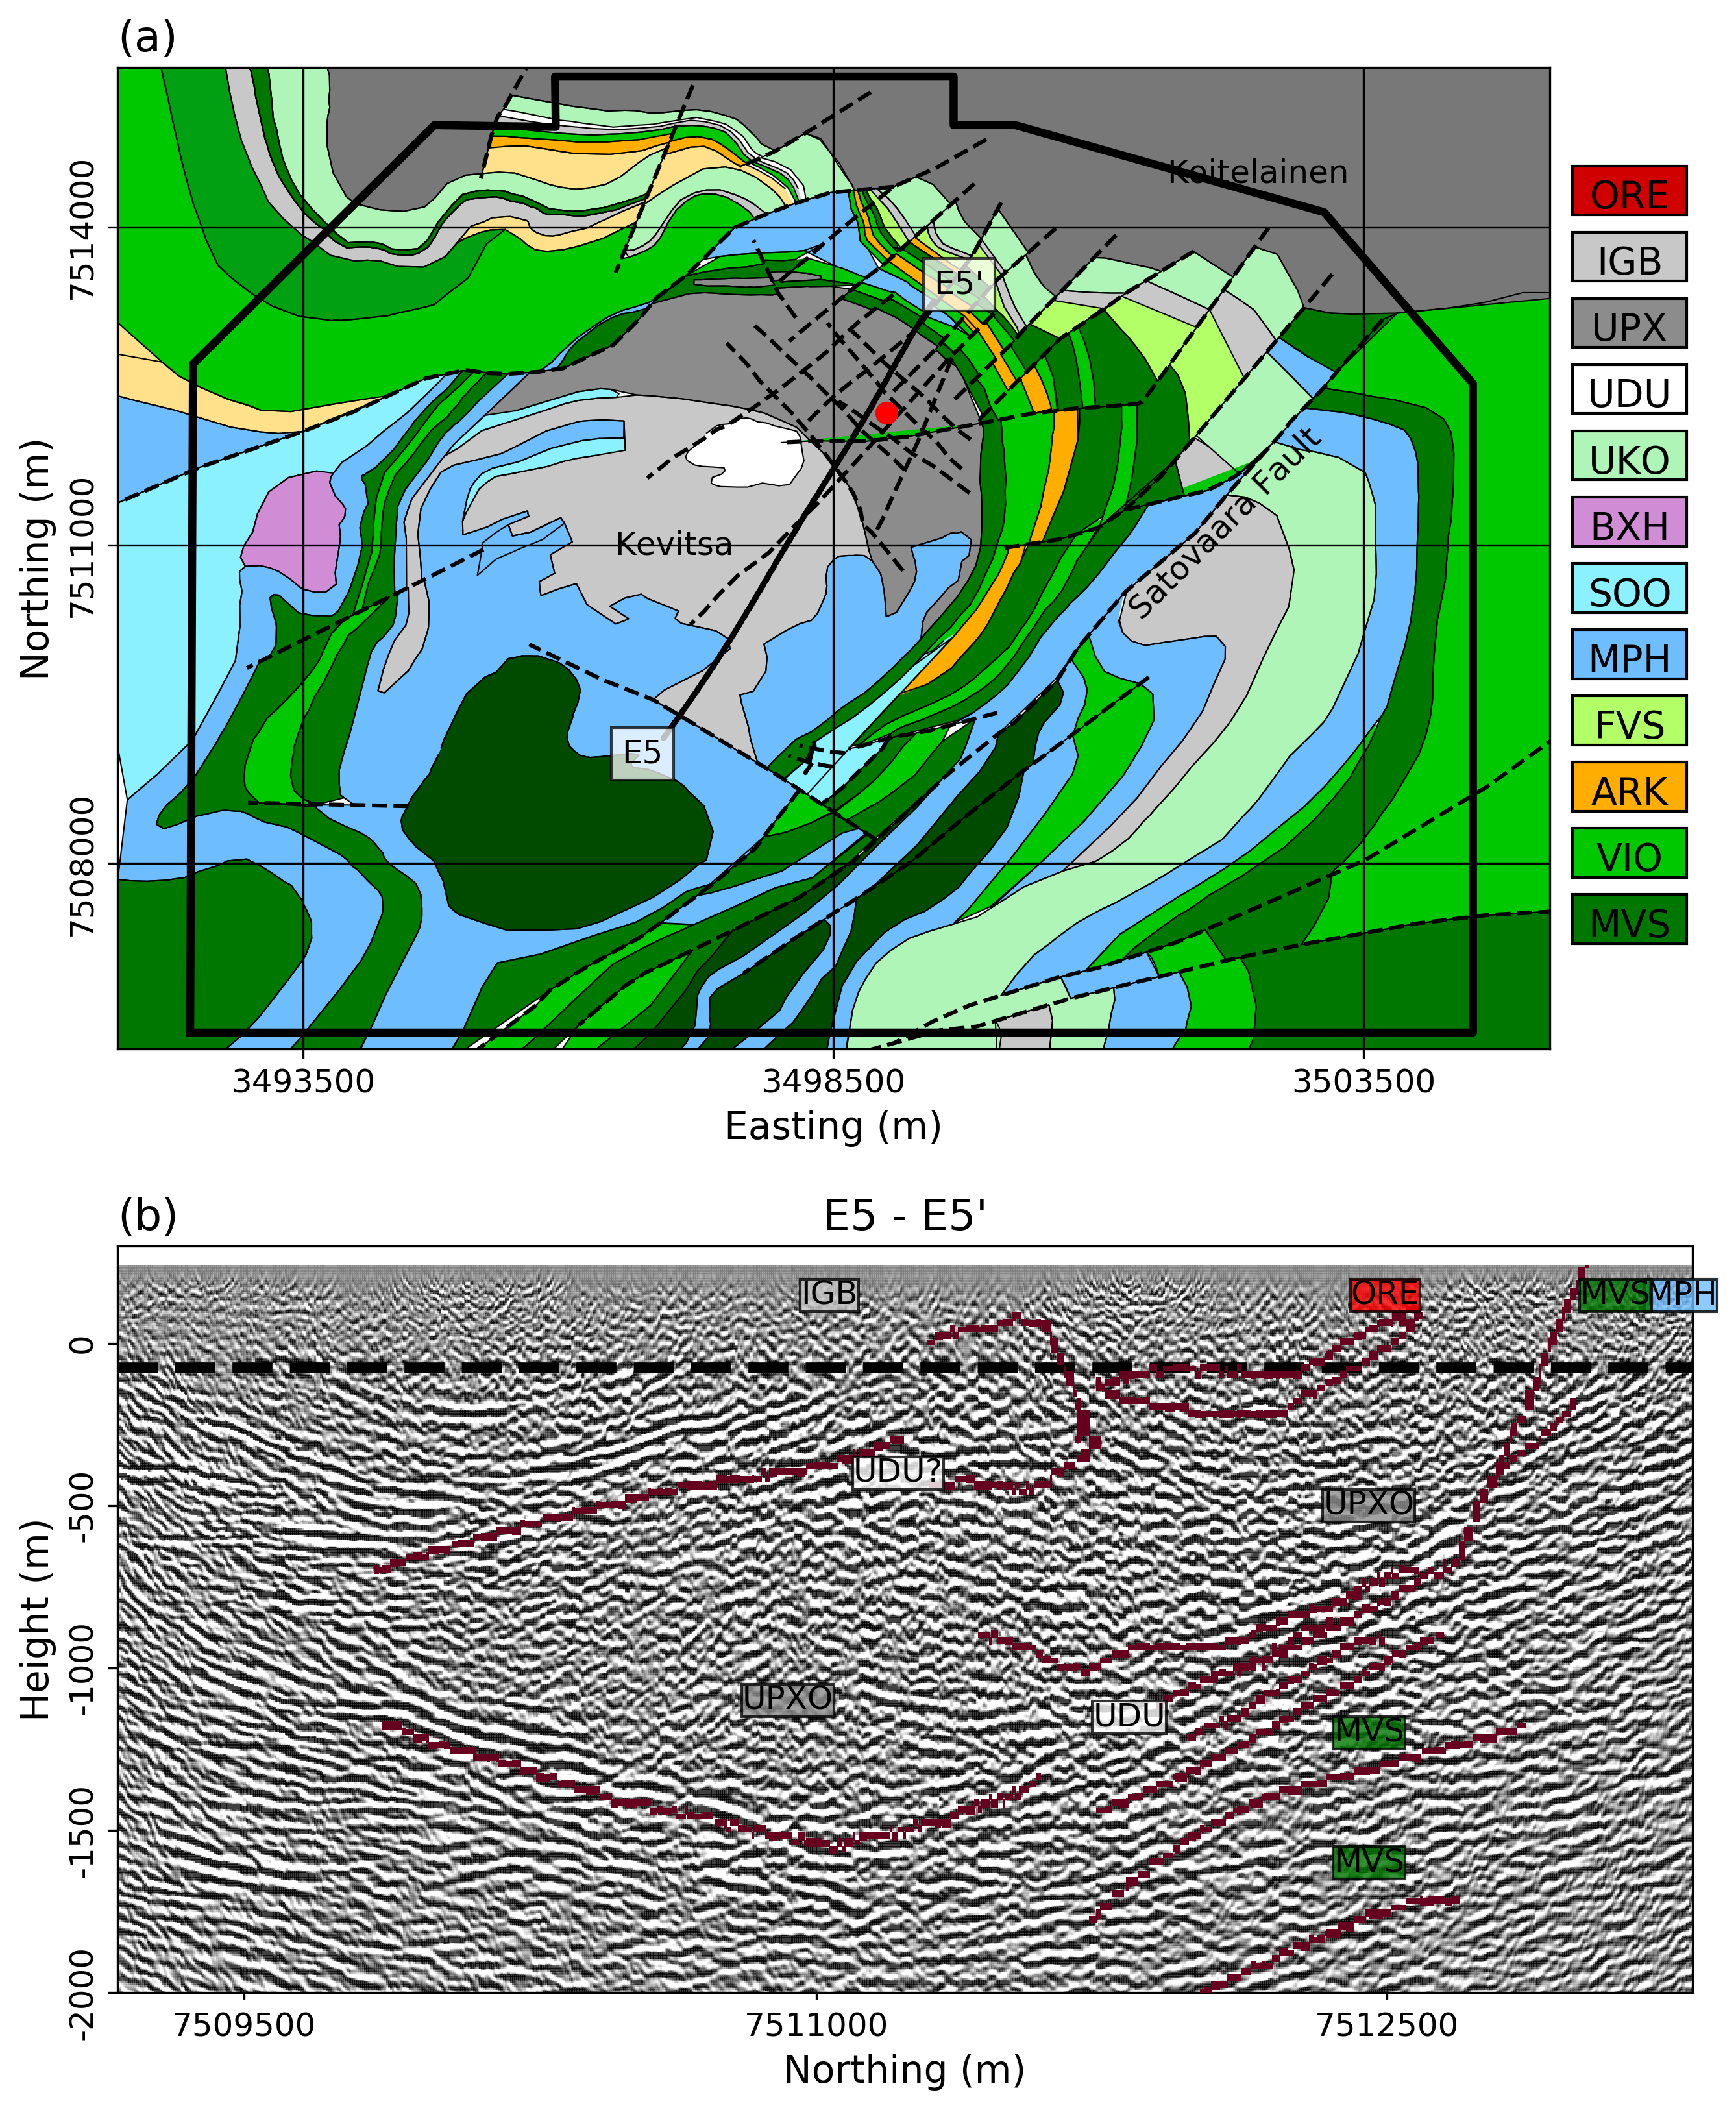
\includegraphics[width=\columnwidth]{Figures/Figure8.png}
\caption{(a) Geological map of the Kevitsa-Satovaara intrusive complex adapted from \cite{Koivisto2015}, with geological definition provided in Table~1. Mapped faults (dash) are shown for reference. (b) 2D seismic line reflection line E5 with interpreted geological contacts between the main reflectors.}
\label{Kevitsa_Geology}
\end{figure}

\begin{figure}[p!]
%\includegraphics[width=0.5\columnwidth]{Figure9.png}
\caption{Whisker plot of magnetic susceptibility measured along 279 boreholes. The coloured boxes have a width scaled by the calculated standard deviation and centered on the mean value for all intercepts belonging to the same lithological classification, as defined in Table~1. The black lines on either side define the minimum and maximum values. The different lithologies are colour coded and grouped based on relative age and similarities in physical properties.}
\label{Kevitsa_PhysProp}
\end{figure}

\begin{figure}[p!]
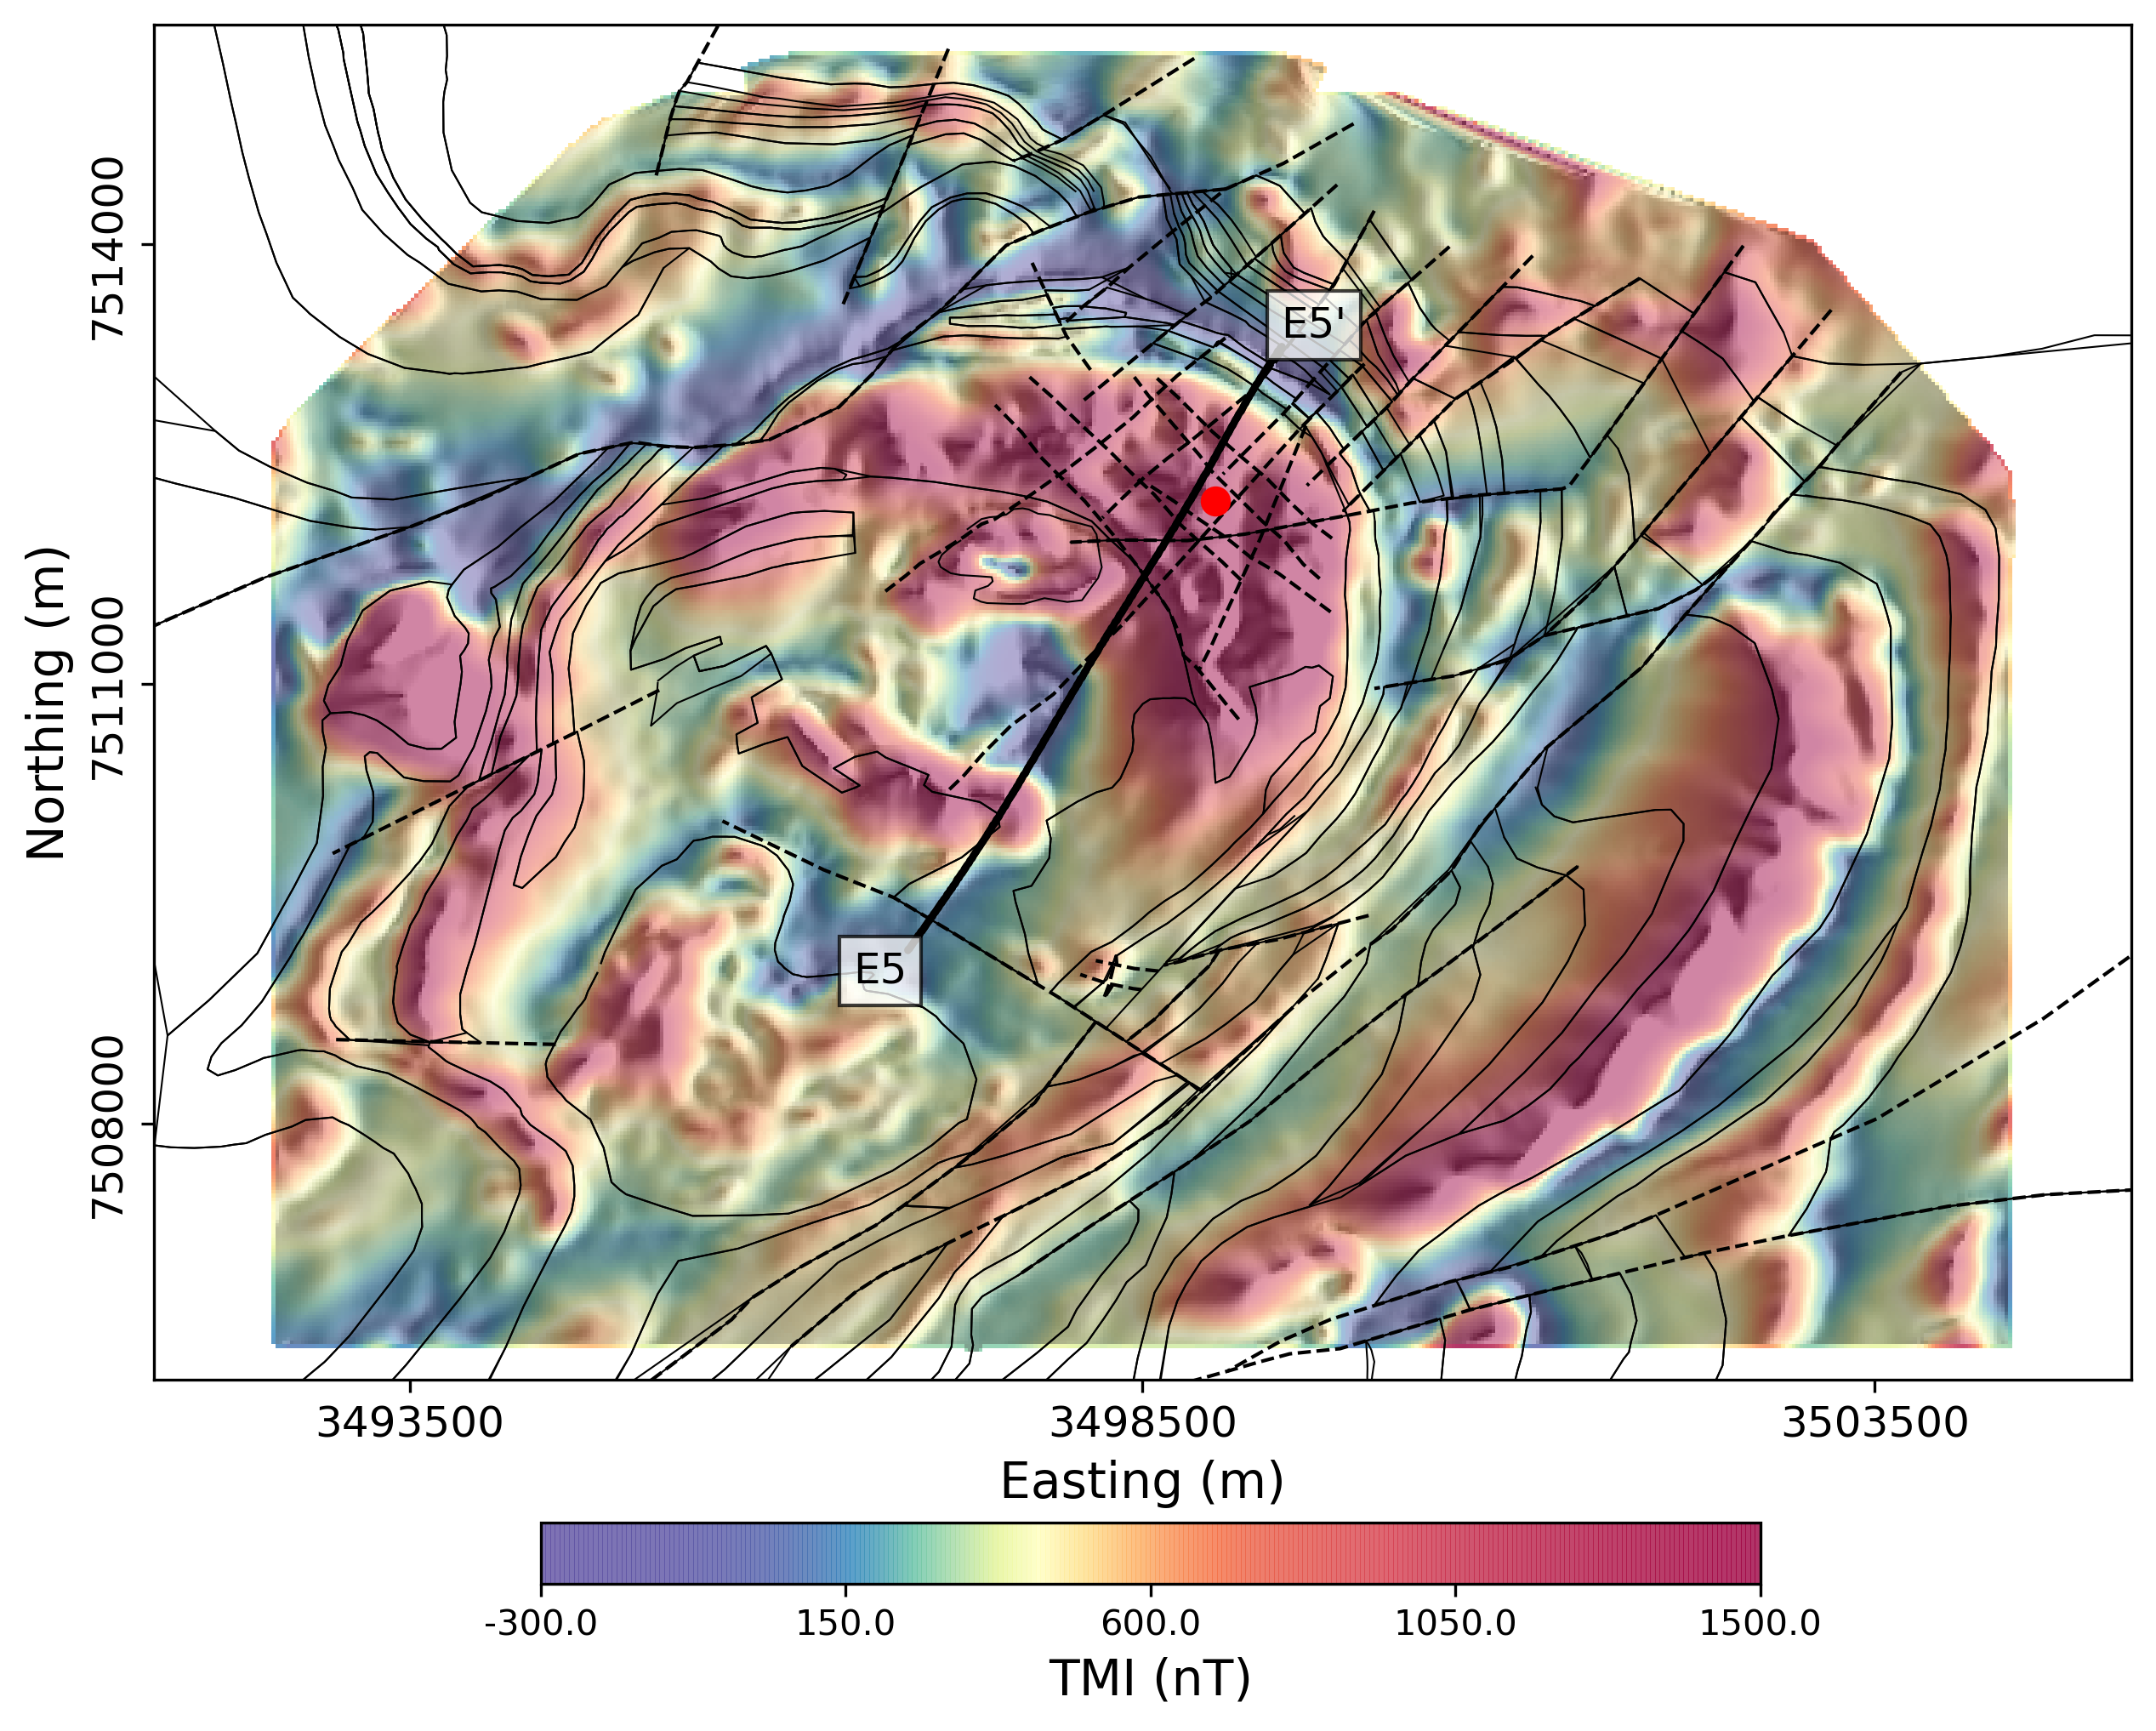
\includegraphics[width=\columnwidth]{Figures/Figure10.png}
\caption{Observed TMI data over the Kevitsa intrusion with histogram equalized color scale. Geological contacts (black), faults (dash) identified from surface mapping and the 2D seismic line locations E5, are shown for reference. Sun shading from east is added to highlight subtle features (Azimuth: $270^\circ$, Dip: $45^\circ$).}
\label{Kevitsa_TMI}
\end{figure}

\begin{figure}[p!]
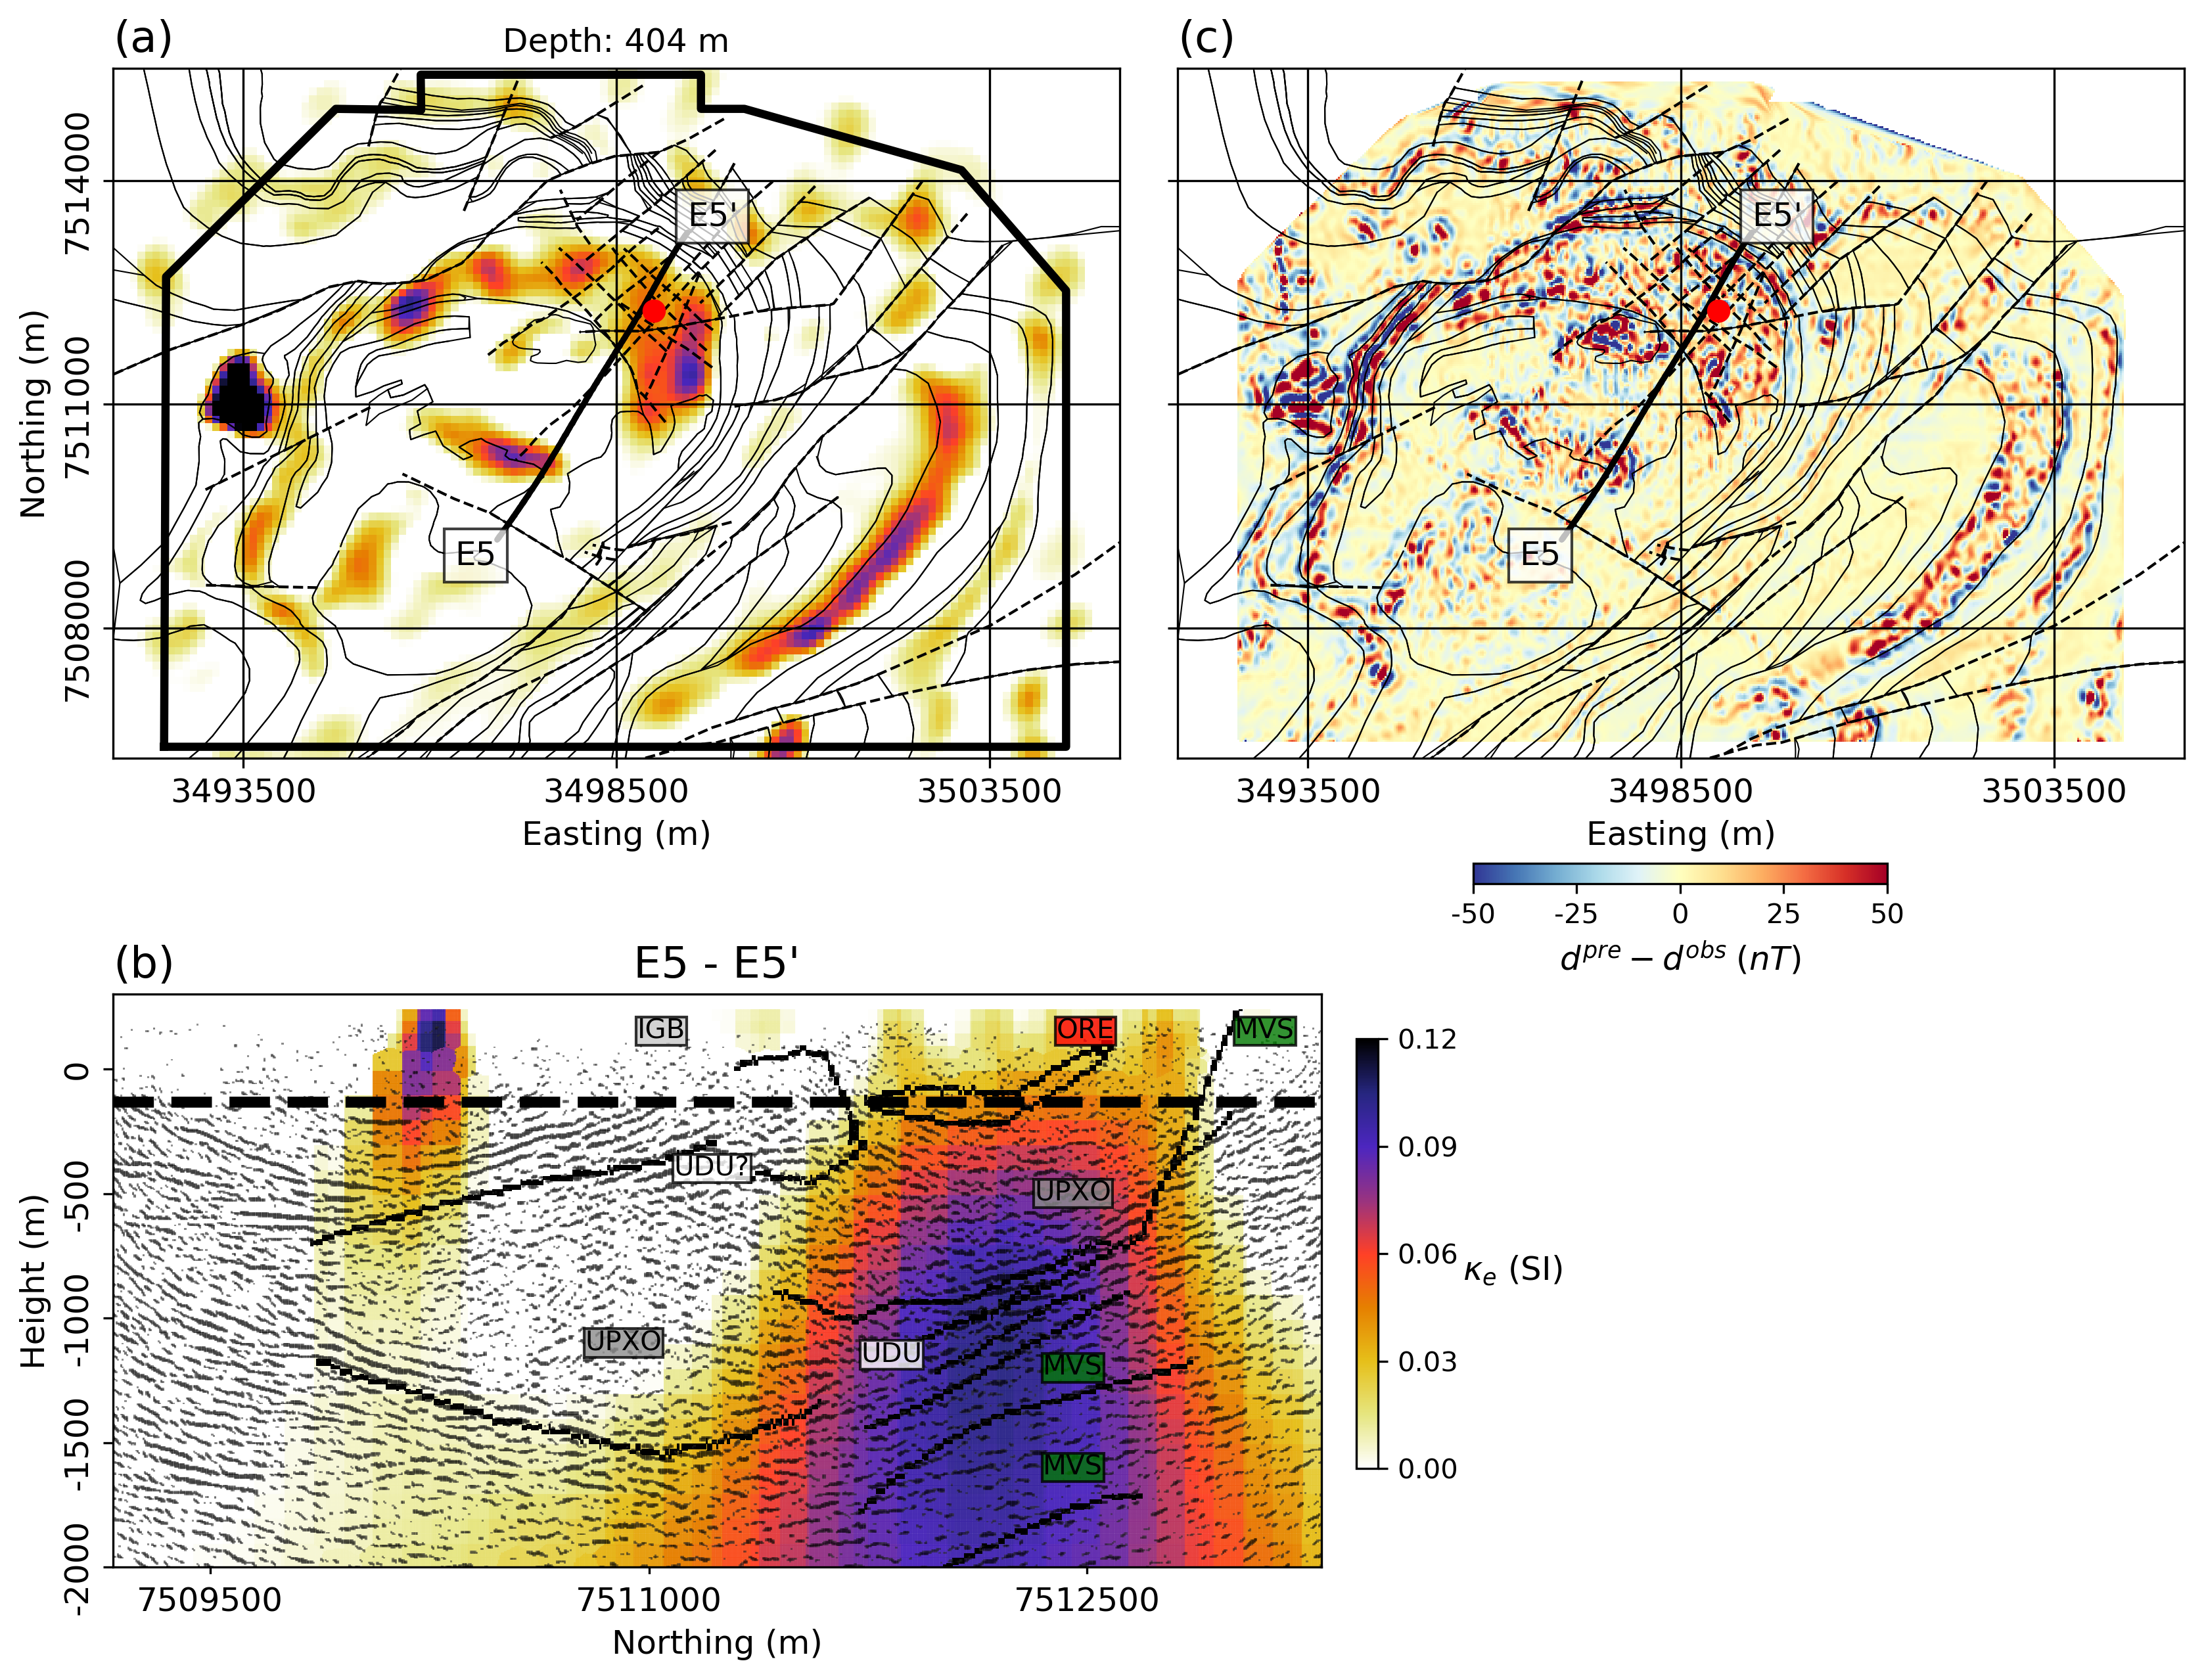
\includegraphics[width=\columnwidth]{Figures/Figure11.png}
\caption{(a) Horizontal and (b) vertical sections through the recovered susceptibility model that ignores the effect of remanence. Lithological contacts (black) identified by \cite{Koivisto2015} are shown for reference. (c) The residual map shows strong correlation with the negative magnetic data.}
\label{MAG_lp_EW}
\end{figure}

\begin{figure}[p!]
\includegraphics[width=\columnwidth]{Figures/Figure12.png}
\caption{Horizontal sections at $\approx$ 300 m below topography for a suite of models using various sparsity assumptions put on the amplitude of magnetization for $p_s\;, p_{x,y,z} \in [0,\: 2]$. Norm measure on the magnetization angle are fixed to $p_{x,y,z}=0$ in order to promote uniform magnetization direction.}
\label{MVIS_Hsections}
\end{figure}

\begin{figure}[p!]
\includegraphics[width=\columnwidth]{Figures/Figure13.png}
\caption{Vertical sections along the E5 seismic reflection line for a suite of models using various sparsity assumptions put on the amplitude of magnetization for $p_s\;, p_{x,y,z} \in [0,\: 2]$. Norm measure on the magnetization angle are fixed to $p_{x,y,z}=0$ in order to promote uniform magnetization direction.}
\label{MVIS_Vsections}
\end{figure}

\begin{figure}[p!]
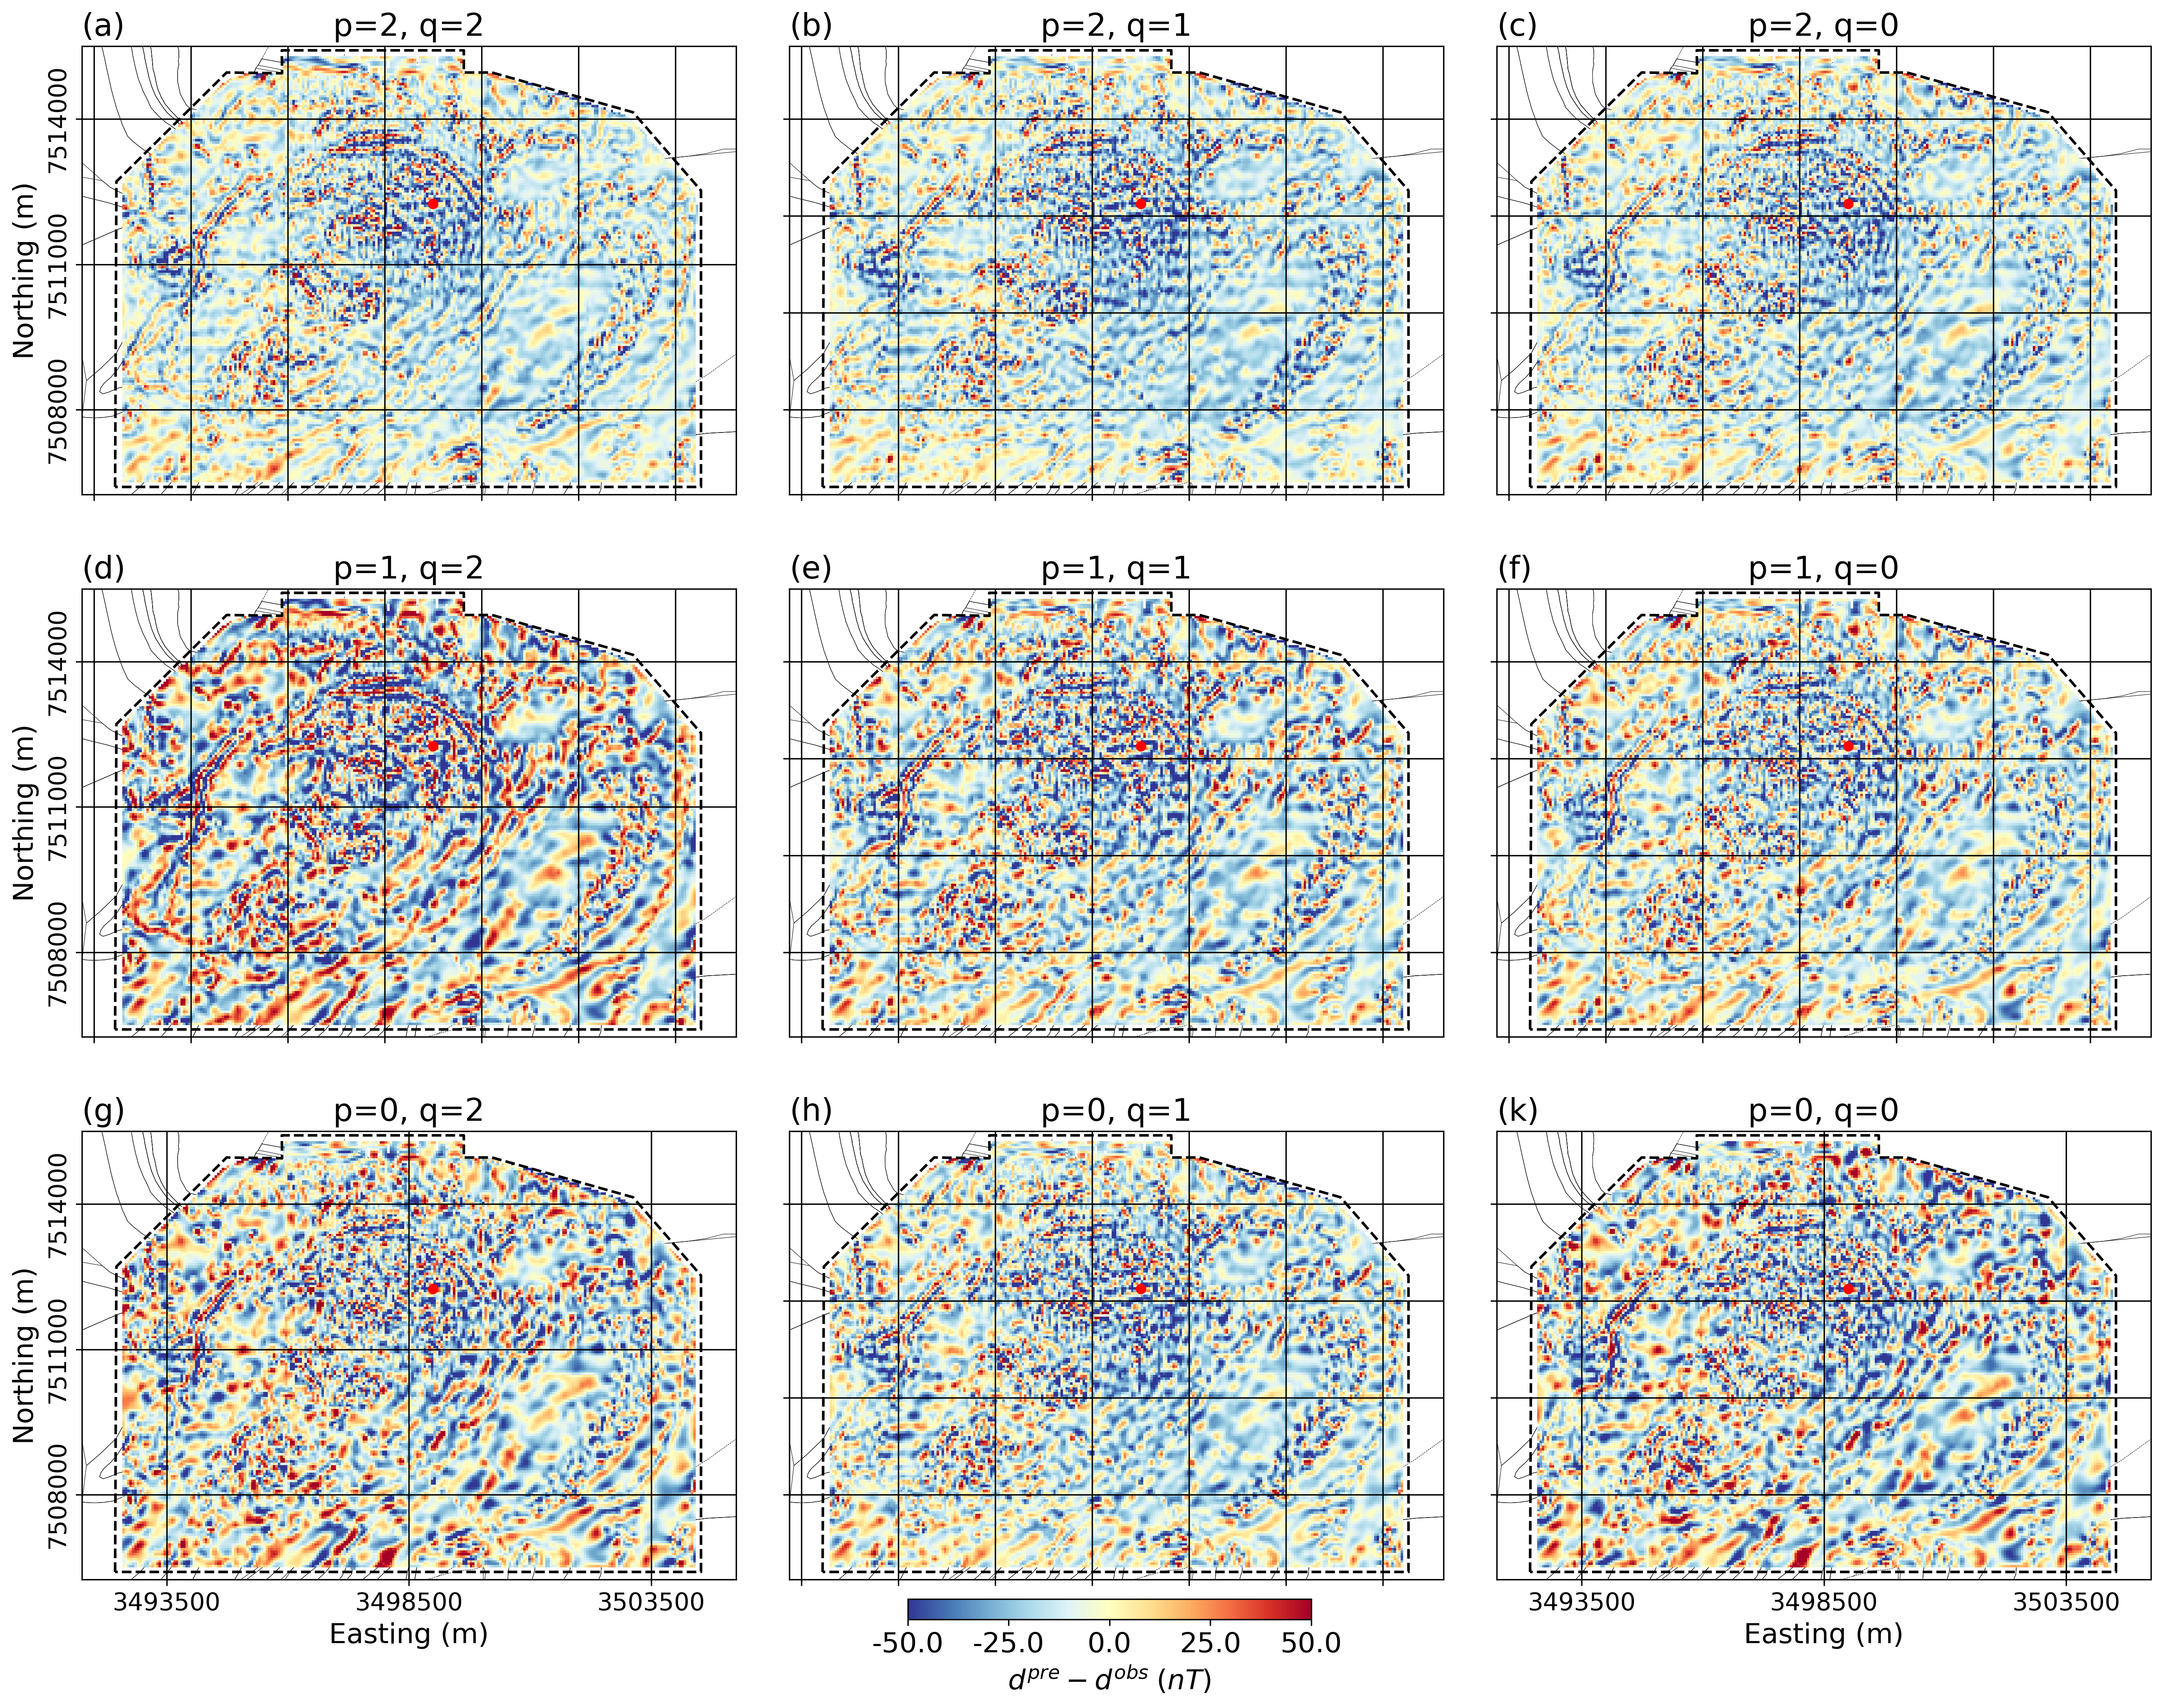
\includegraphics[width=\columnwidth]{Figures/Figure14.png}
\caption{Residual data maps for the nine inversions shown in Figure~\ref{MVIS_Hsections} and \ref{MVIS_Vsections}.}
\label{MVIS_predicted}
\end{figure}

\begin{figure}[p!]
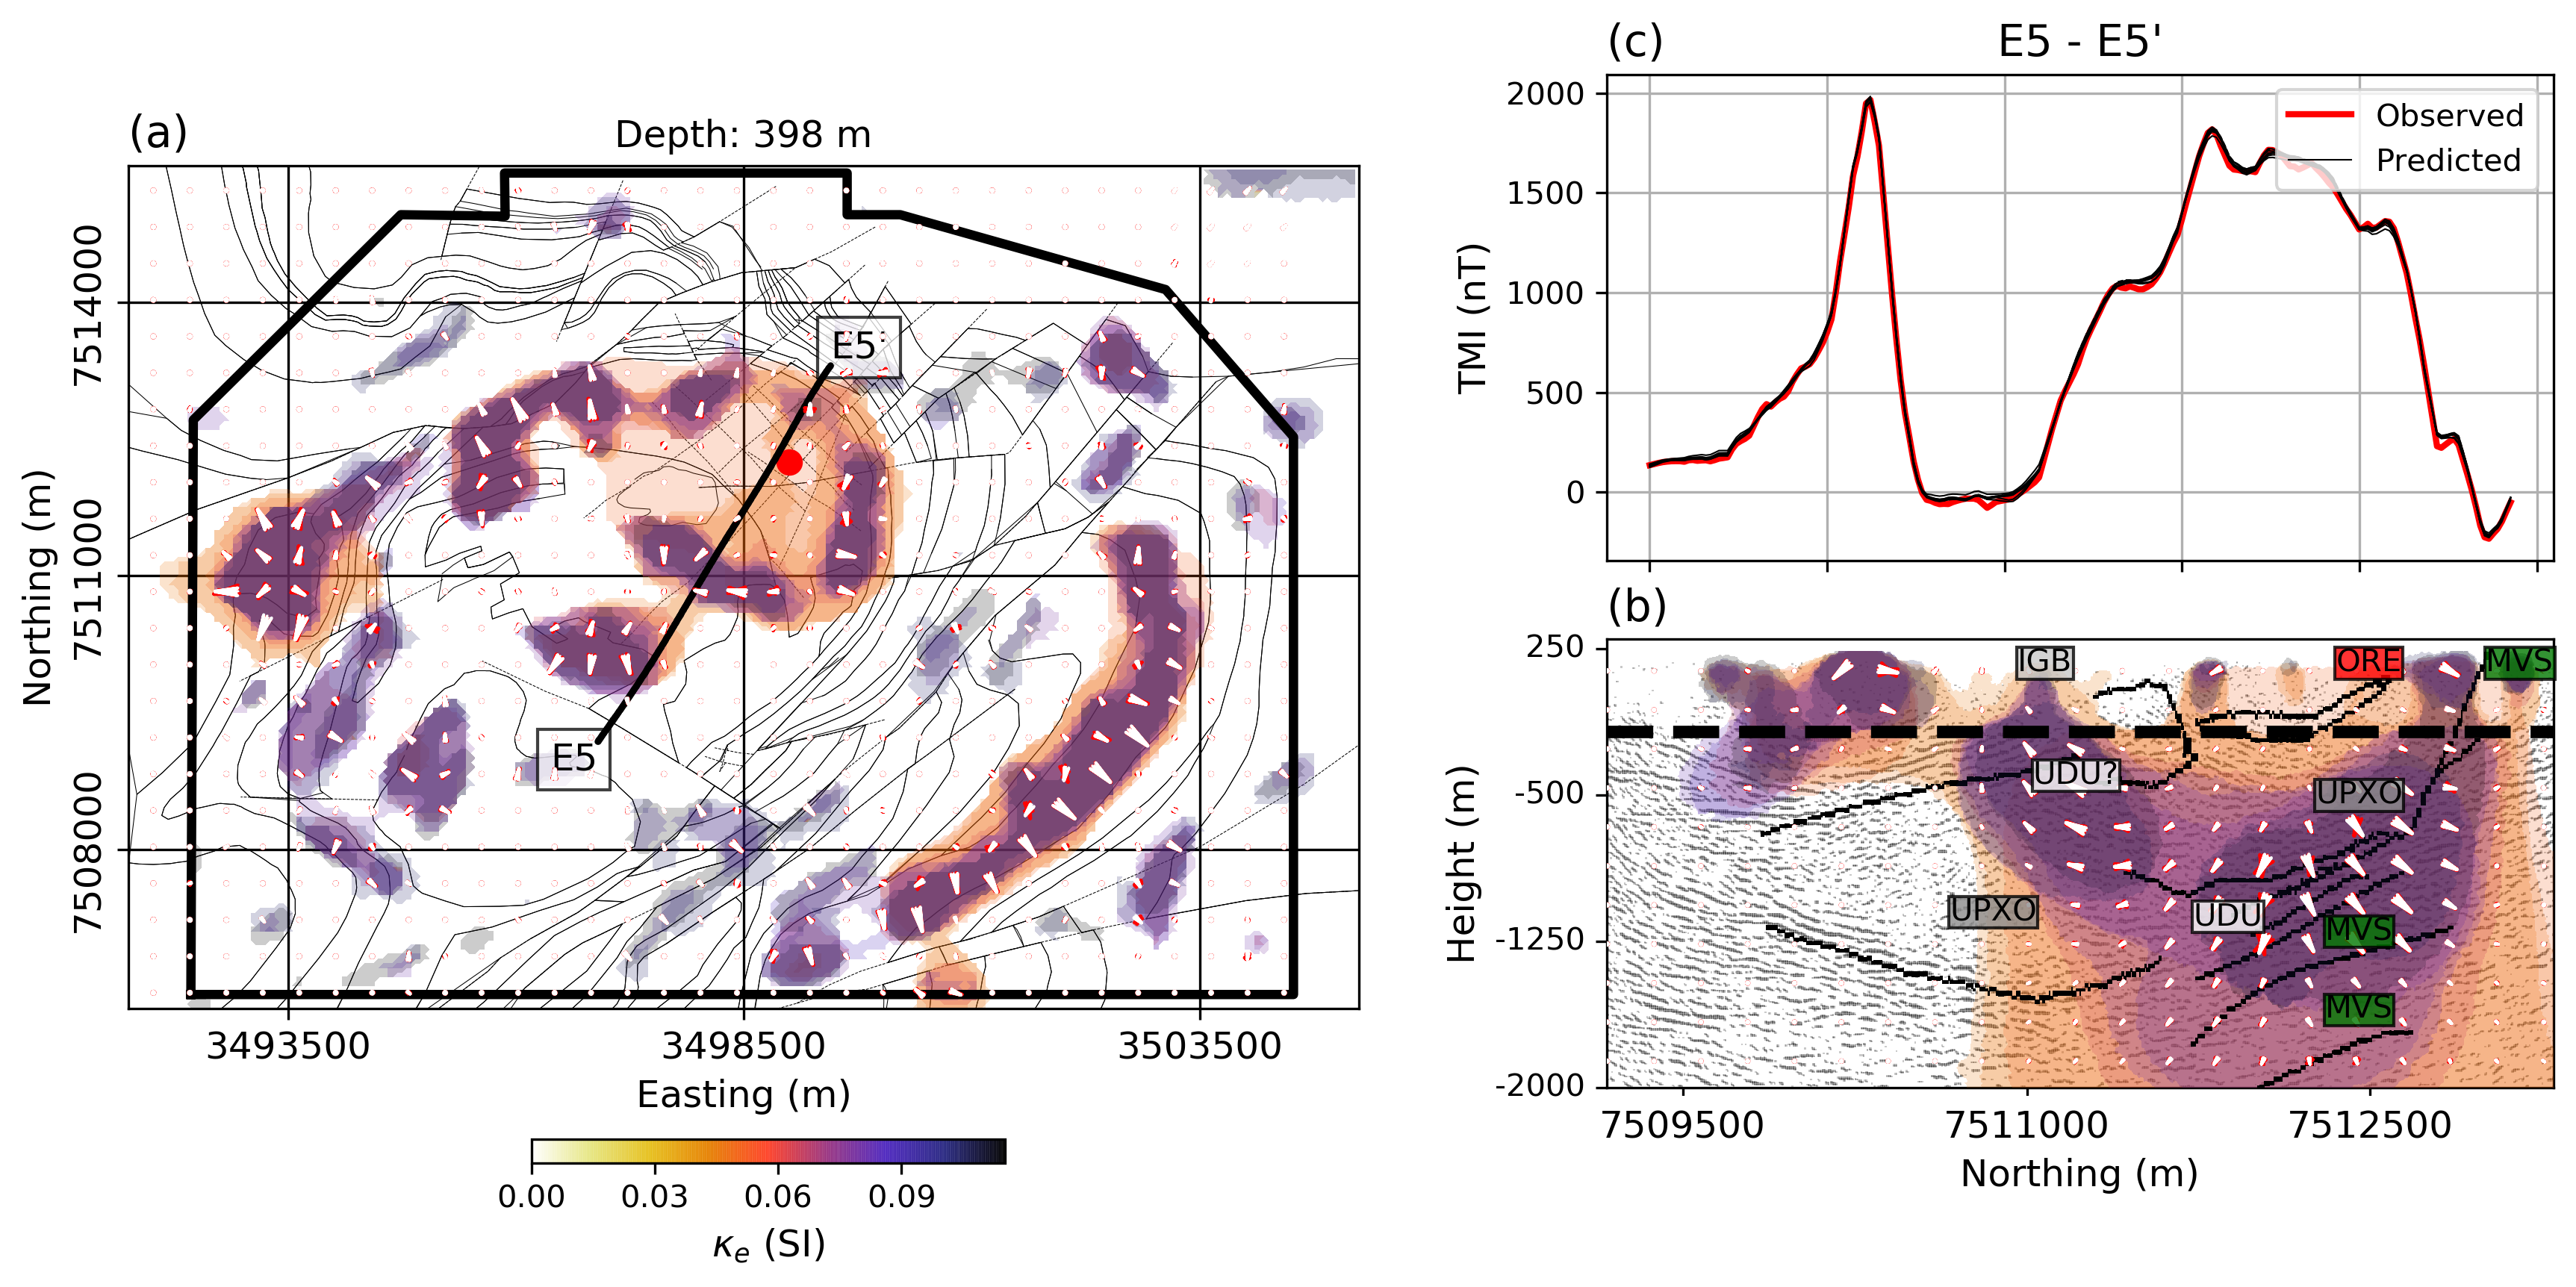
\includegraphics[width=\columnwidth]{Figures/Figure15.png}
\caption{(a) Horizontal and (b) vertical sections through iso-contours of magnetization recovered from nine mixed $\ell_p$-norm inversions. Magnetization orientation (white arrowheads) and standard deviation on the angle (red arrowheads) are shown. (c) Data profile along the E5 section for the observed and predicted data calculated from the recovered models.}
\label{MVIS_Iso_model}
\end{figure}

\end{document}



\bibliography{references}
\bibliographystyle{seg}

%\listoffigures
\pagebreak
%\listoftables

\begin{table}
\caption{Intervals along boreholes KV200 and KV297 reporting significant remanent magnetization.}
\label{Table1}
\end{table}

\begin{table}
\caption{Summary table grouping the various lithological units logged from boreholes. Expected magnetic susceptibility contrasts are derived from Figure~\ref{Kevitsa_PhysProp}.}
\label{Table2}
\end{table}

\pagebreak

\begin{figure}[p!]
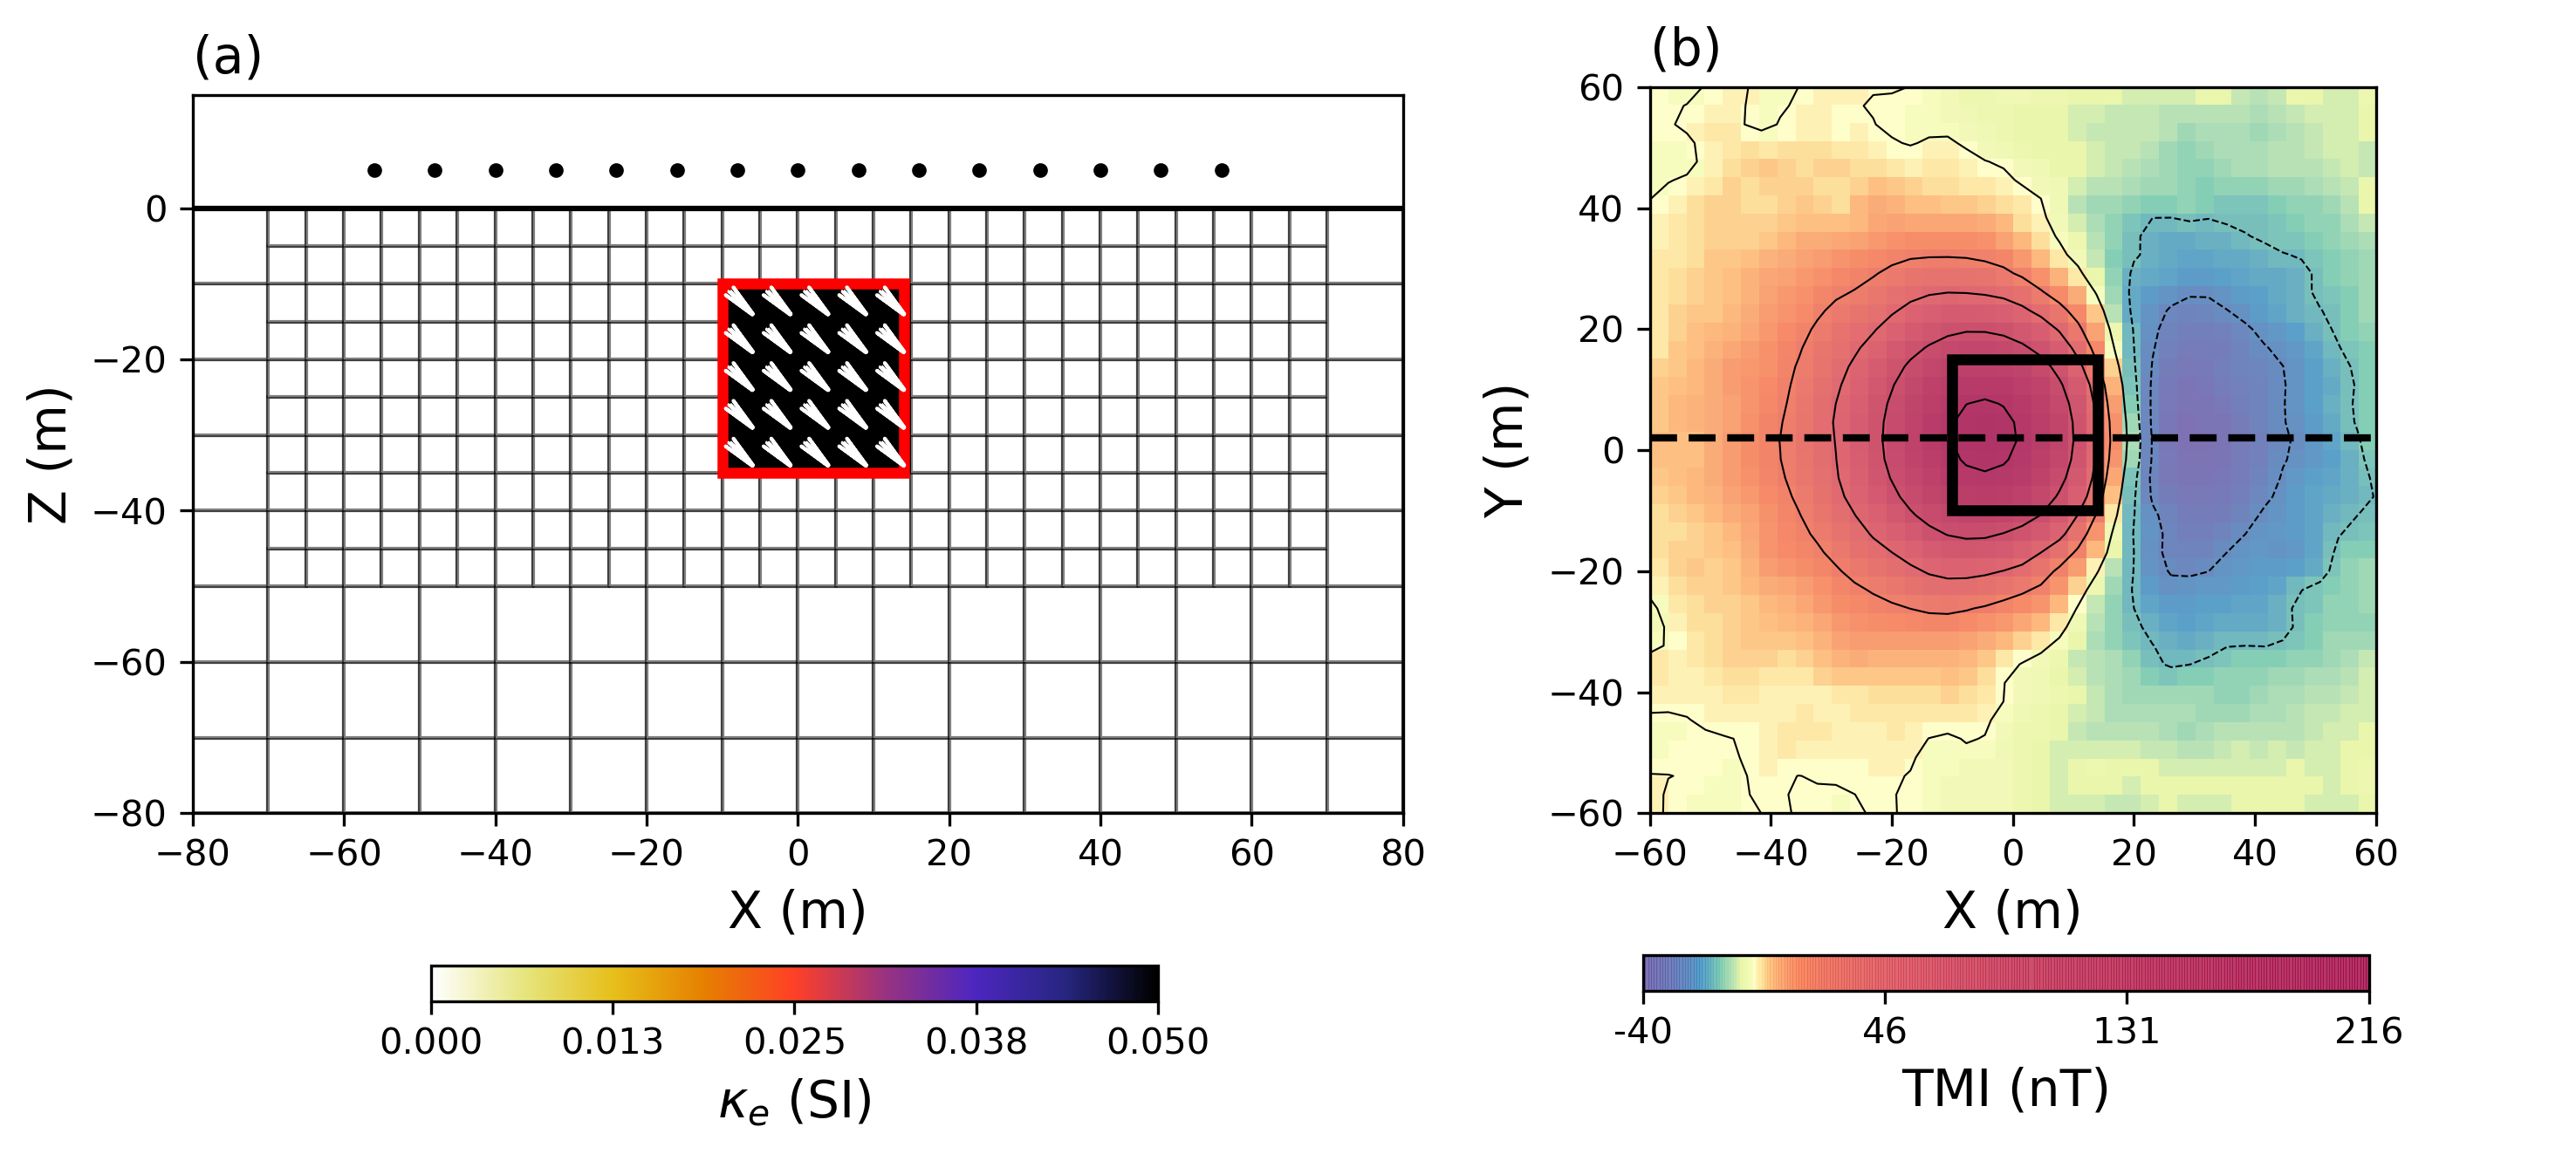
\includegraphics[width=\columnwidth]{Figures/Figure1.png}
\caption{(a) Vertical section through the synthetic block model (Y = 0 m) with magnetization $\mathbf{M}$ [$2.0\: A/m,\; I: 45^\circ,\; D: 90^\circ$]($\kappa_e$ = 0.05 SI). Survey points (black dots) are placed 15 m above the magnetic anomaly. (b) Simulated TMI data map with random Gaussian noise added, 1 nT standard deviation. The horizontal position of the block is shown in black for reference.}
\label{REM_model}
\end{figure}

\begin{figure}[p!]
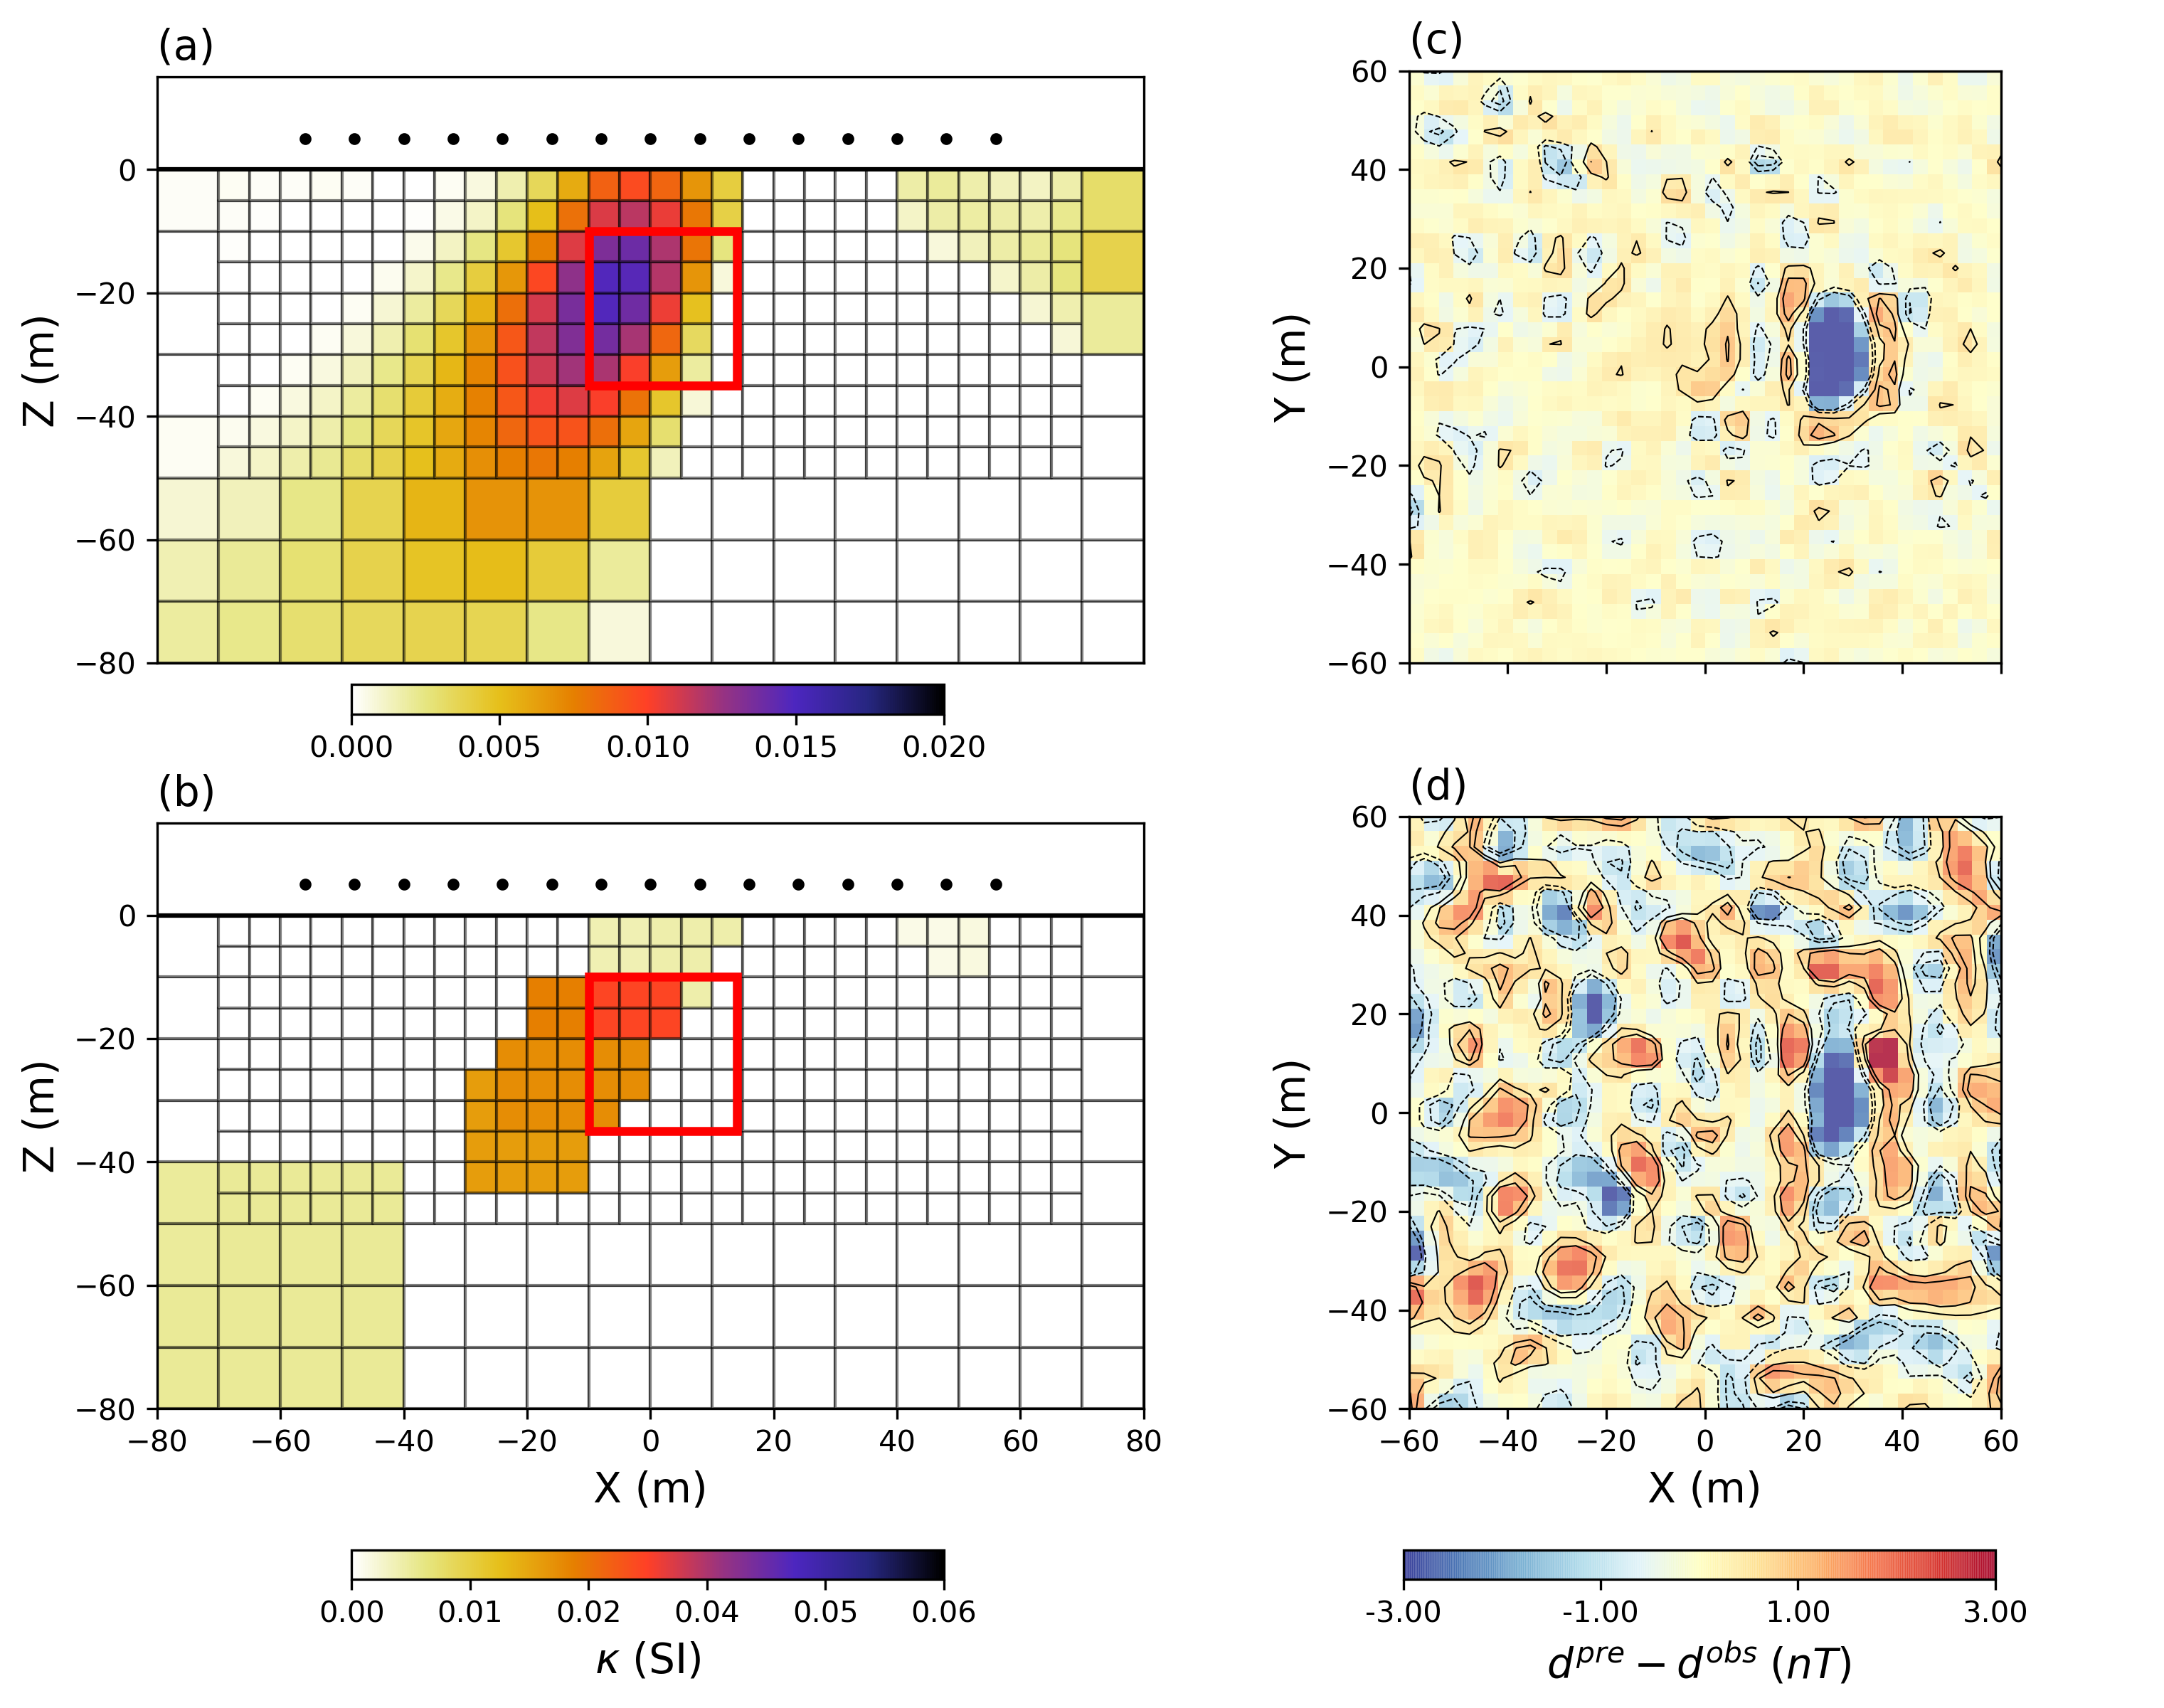
\includegraphics[width=\columnwidth]{Figures/Figure2.png}
\caption{Vertical section through the recovered susceptibility model using (a) smooth assumption ($p_s, \;p_x,\; p_y,\; p_z = 2$) and (b) sparse $\ell_p$-norms to recover a compact model ($p_s,\;p_x,\; p_y,\; p_z = 0$). Both solutions show an anomaly with a false dip due to the wrong assumption of a vertical magnetization. Data residuals for (c) the smooth and (d) compact solution shows correlated signal with the negative data.}\label{Susc_model}
\end{figure}

\begin{figure}[p!]
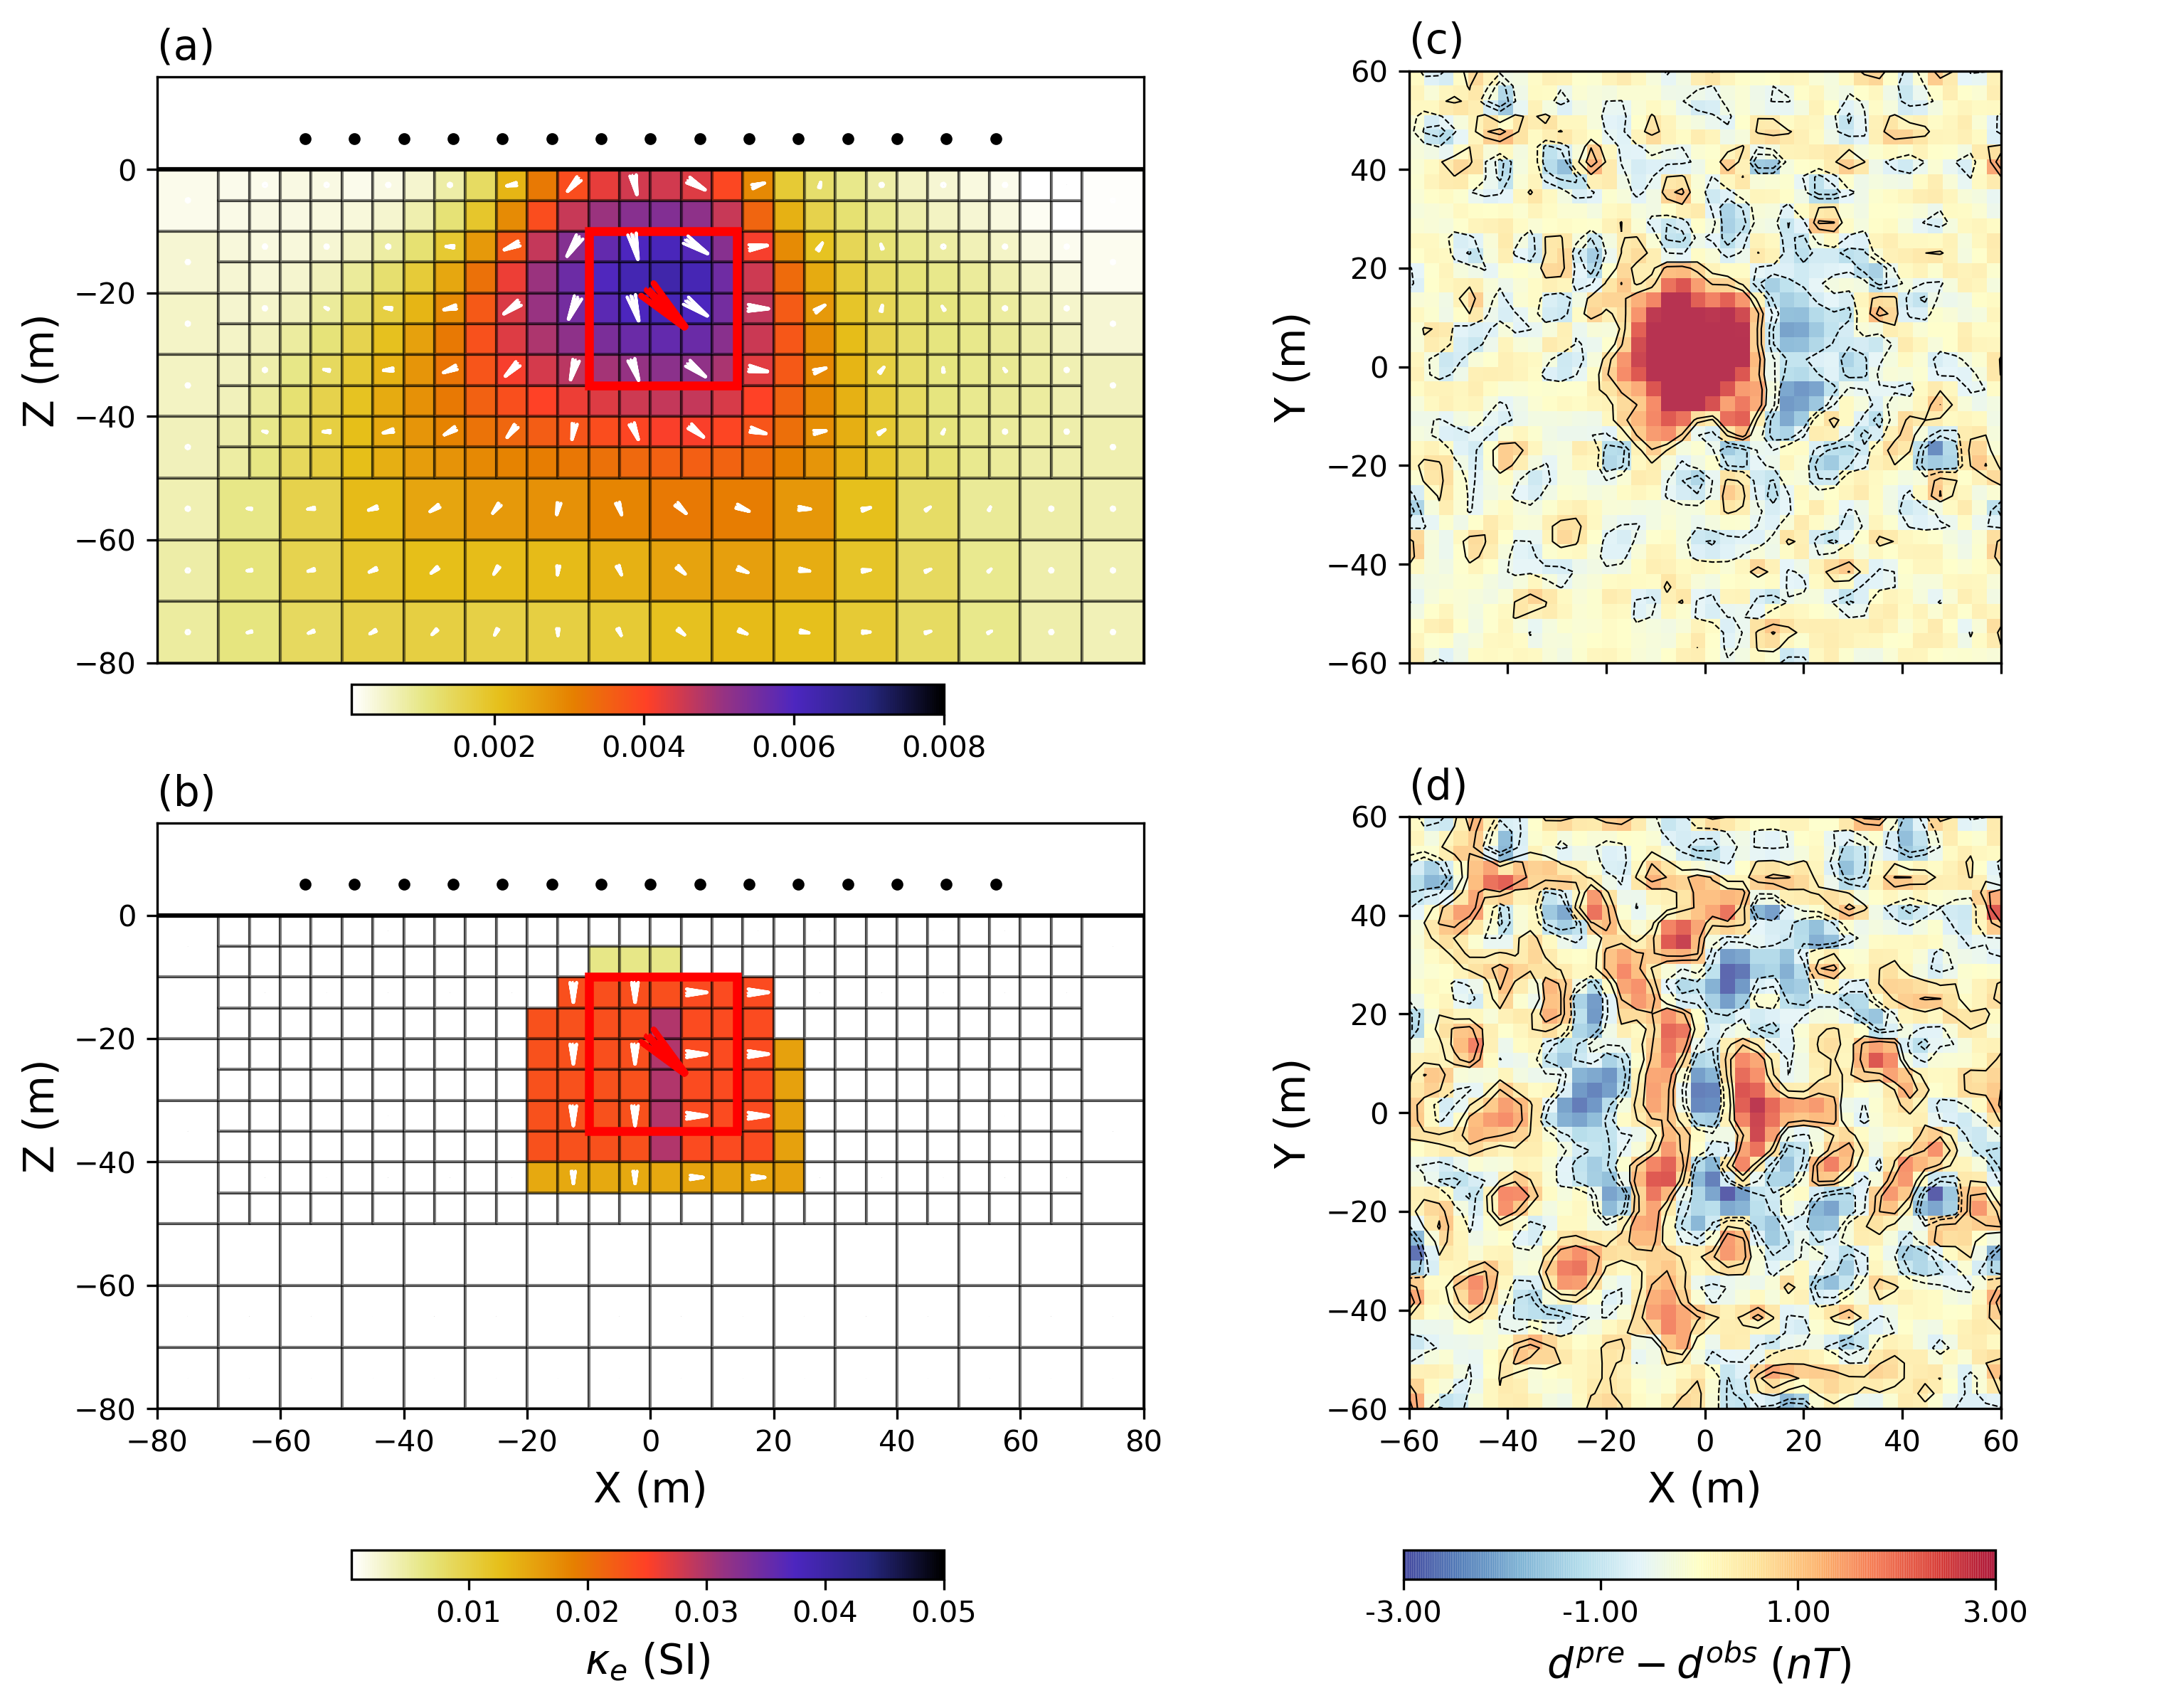
\includegraphics[width=\columnwidth]{Figures/Figure3.png}
\caption{Vertical section through the recovered magnetization vector model using the Cartesian formulation with (a) smooth $l_2$-norm assumption and (b) sparsity constraints applied on all three Cartesian components ($p_{i_s}, \;p_{i_x},\; p_{i_y},\; p_{i_z} = 0$). Color is scaled by the magnitude of magnetization. The true magnetization direction is shown with a red arrow. Data residual map calculated with (c) the smooth and (d) compact solution.}
\label{MVI_C_model}
\end{figure}

\begin{figure}[p!]
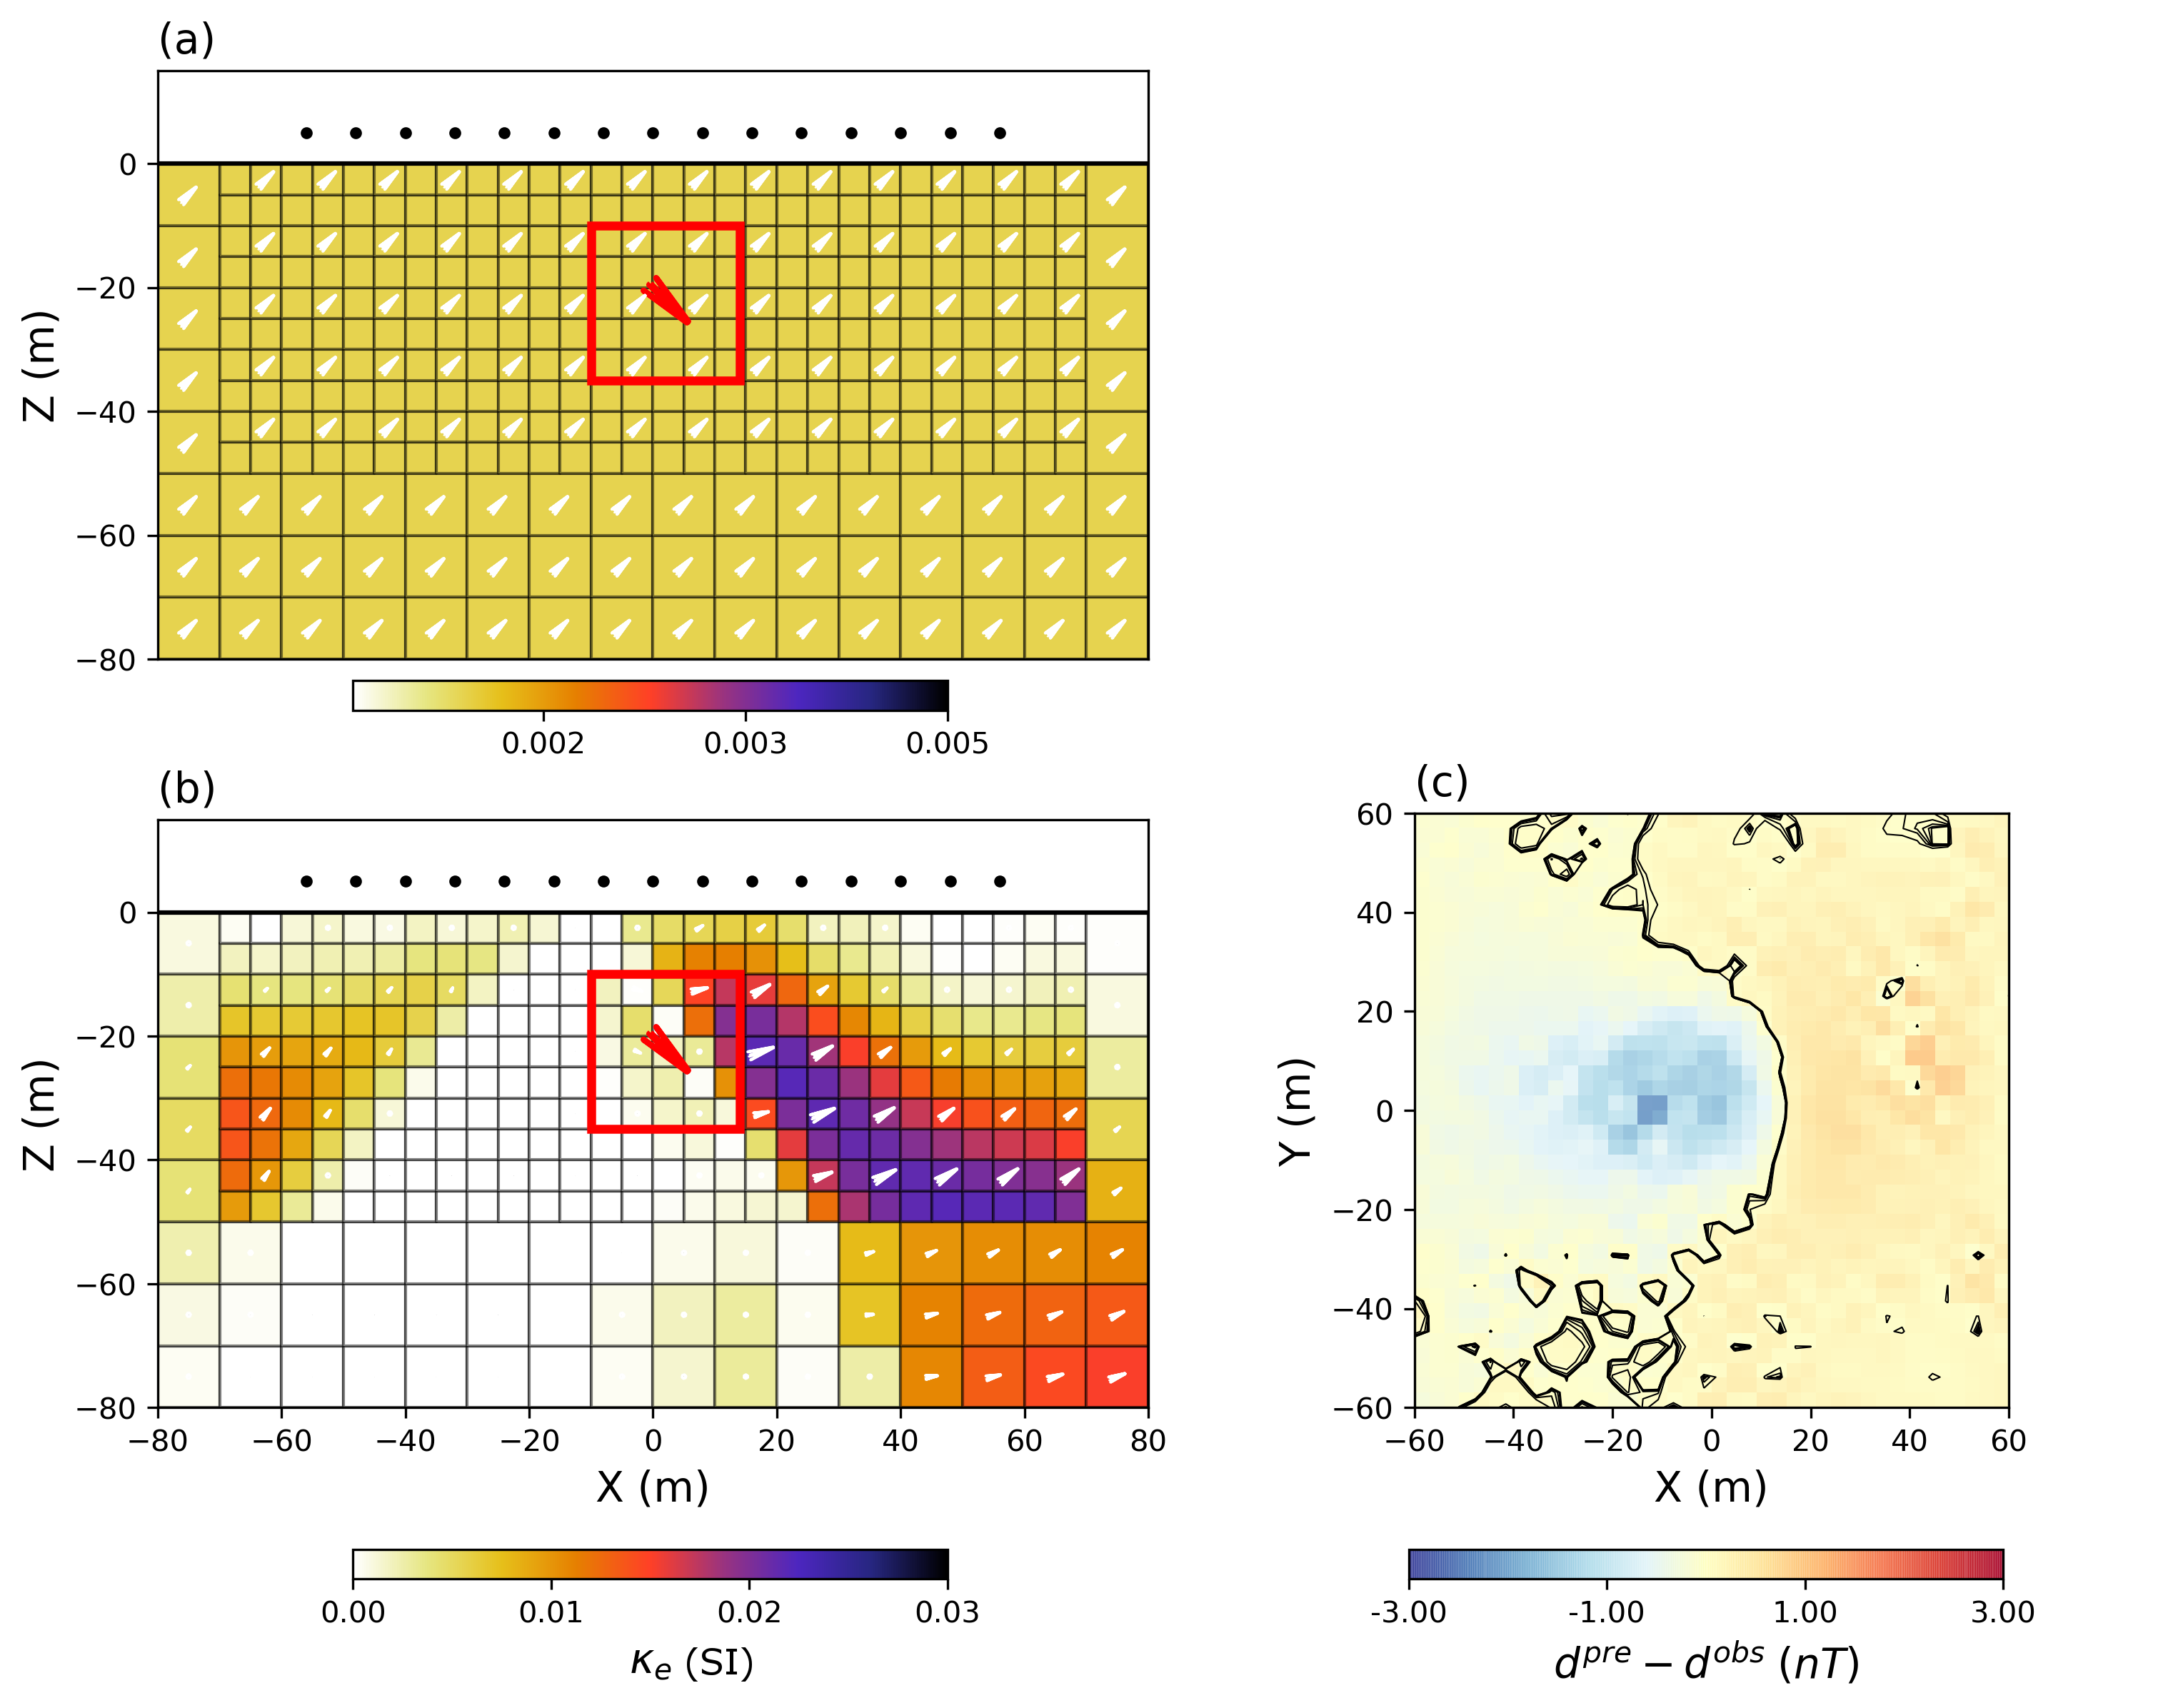
\includegraphics[width=\columnwidth]{Figures/Figure4.png}
\caption{ Vertical section through the (a) starting model and (b) recovered magnetization vector model in spherical coordinates with its (c) data residual map. The inversion stopped after three iterations, unable to further reduce the objective function.}
\label{MVI_S_model_noScale}
\end{figure}

\begin{figure}[p!]
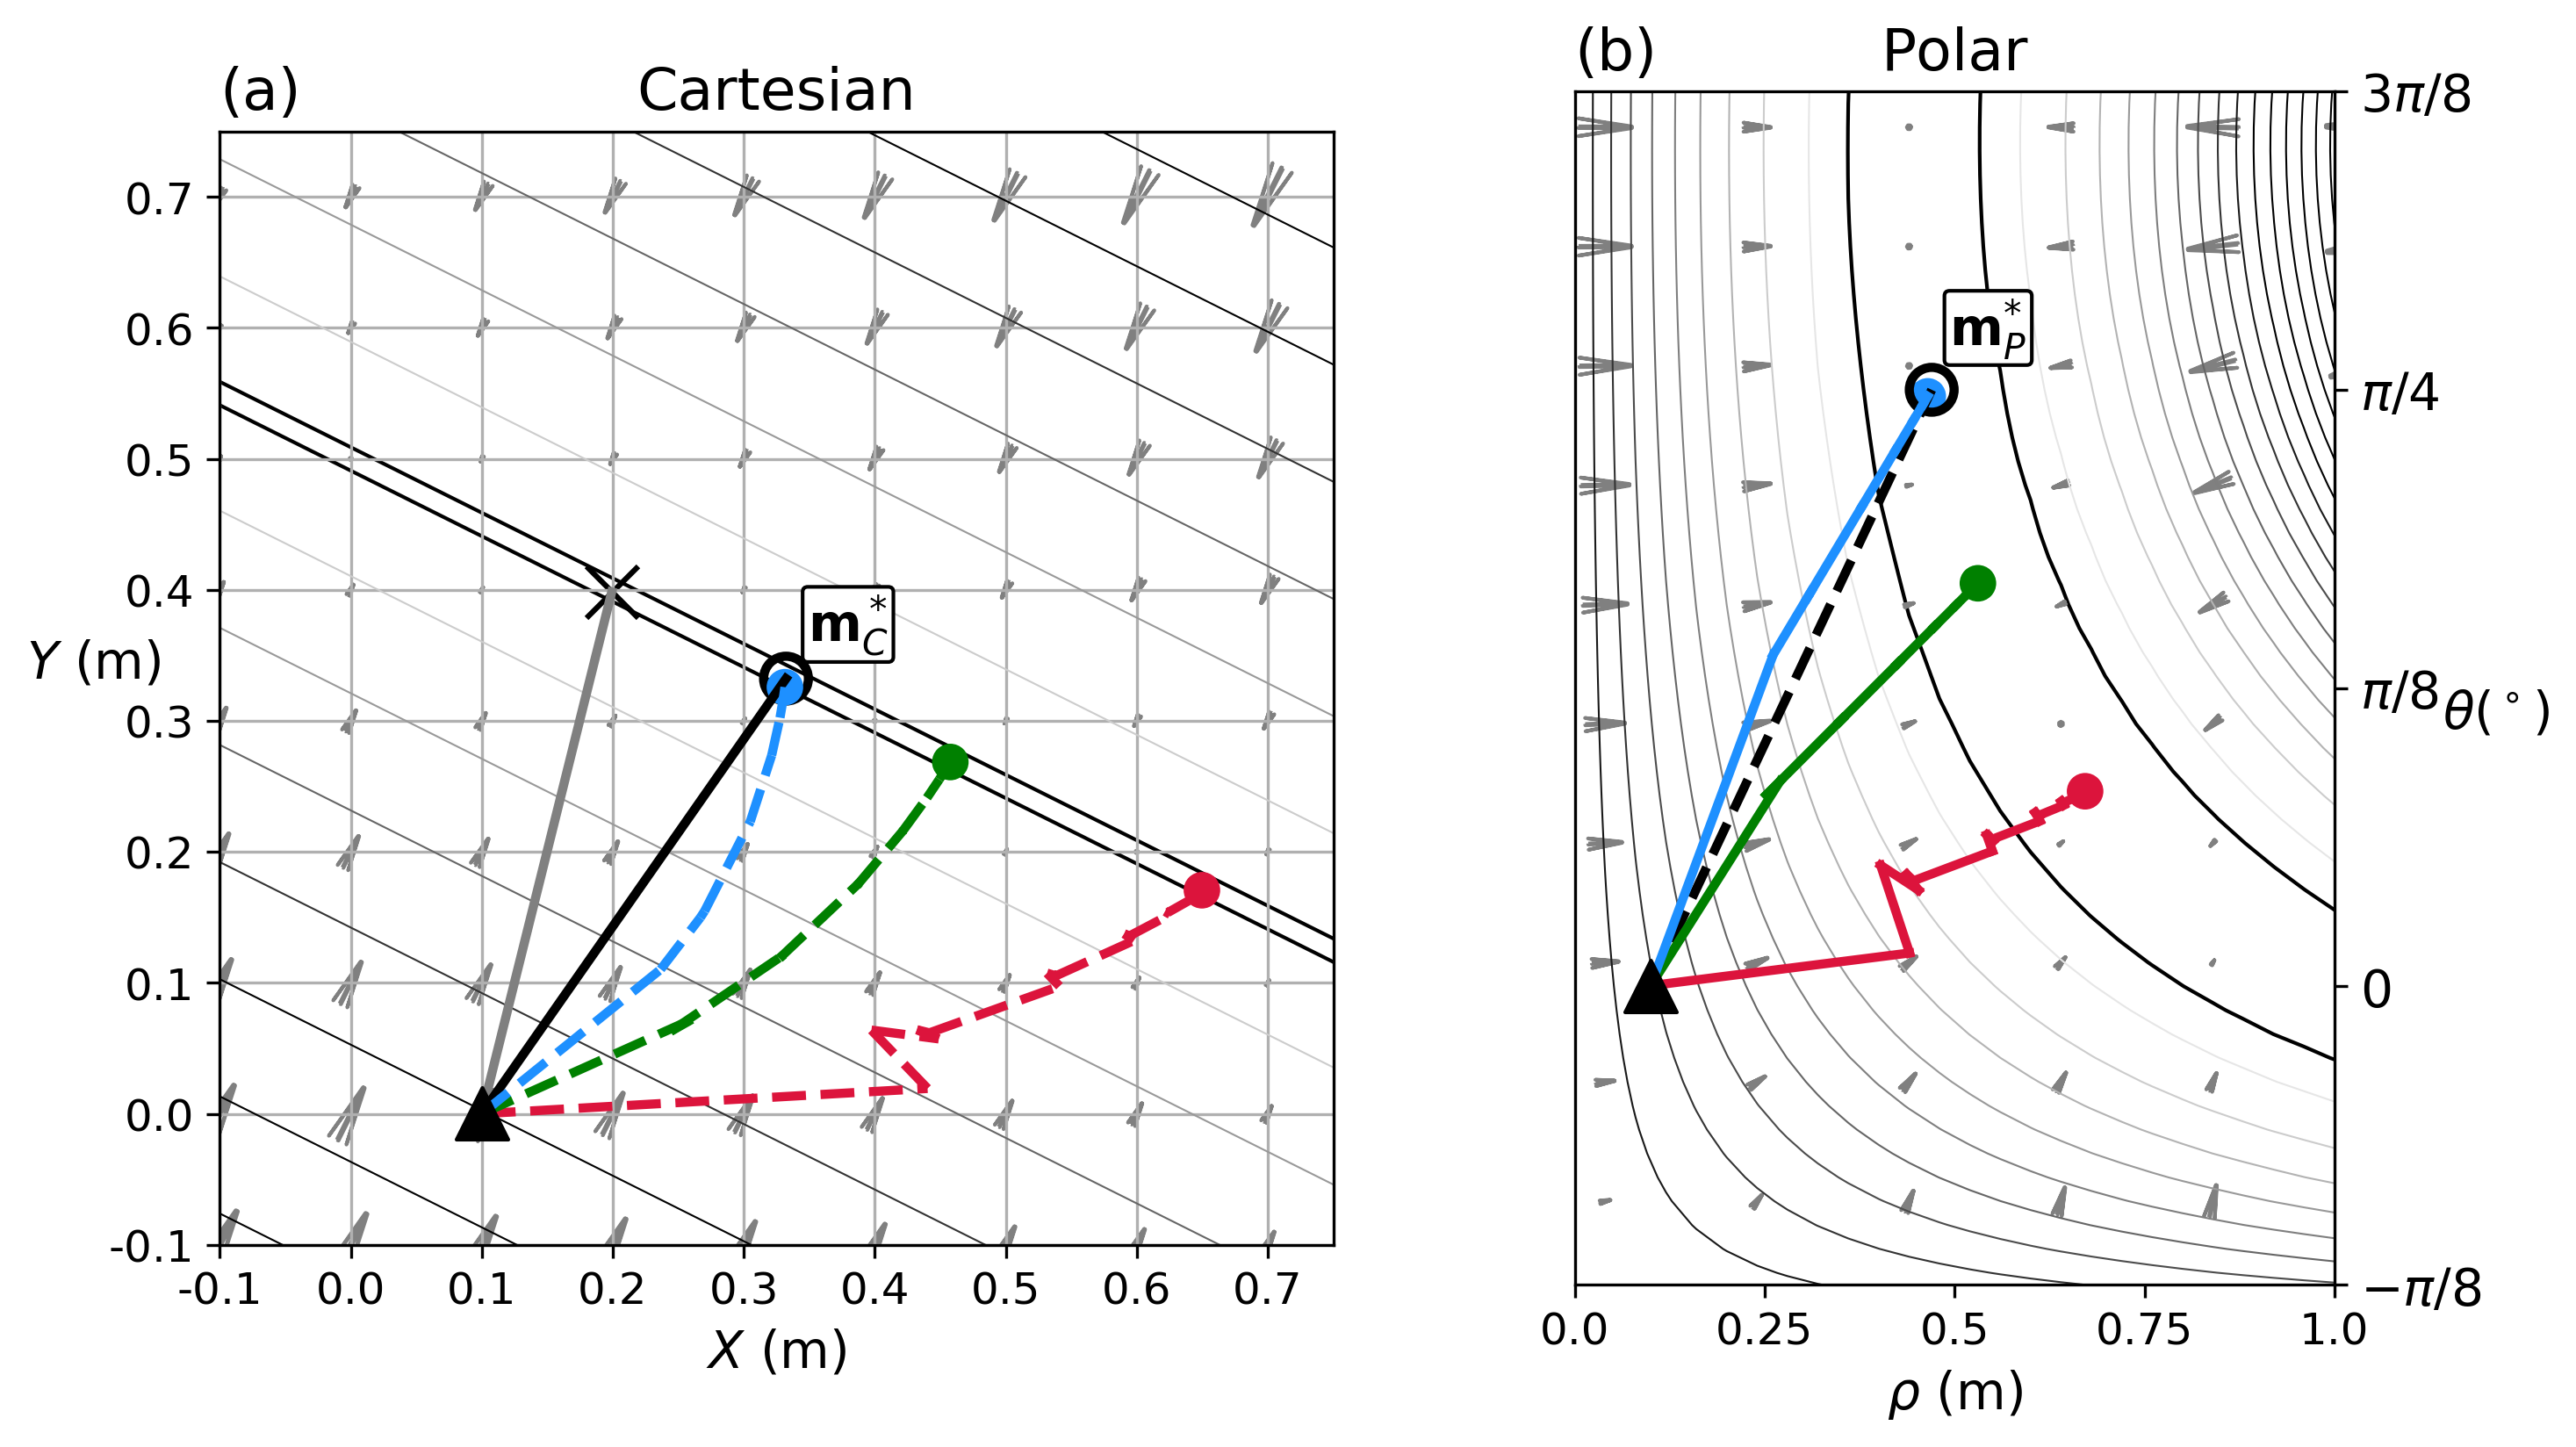
\includegraphics[width=\columnwidth]{Figures/Figure5.png}
\caption{Contour maps for the objective functions of a two-parameter inverse problem solved in (a) Cartesian and (b) polar coordinate systems. Solid colored lines show the model updates taken by different algorithms in their respective coordinate systems and, in dash, the equivalent steps in the other domain for comparison. Each inversion started with the same initial model (triangle). The colors and inversions are: Gray: the non-weighted Cartesian problem; Black: the sensitivity weighted Cartesian problem; Red: the non-linear polar coordinate system with fixed sensitivity weights; Green: the polar problem with iterative sensitivity re-weighting; and Blue: with the added scaling to compensate for the dynamic range of the parameters (see equation~50). }
\label{NonLinearGN}
\end{figure}

\begin{figure}[p!]
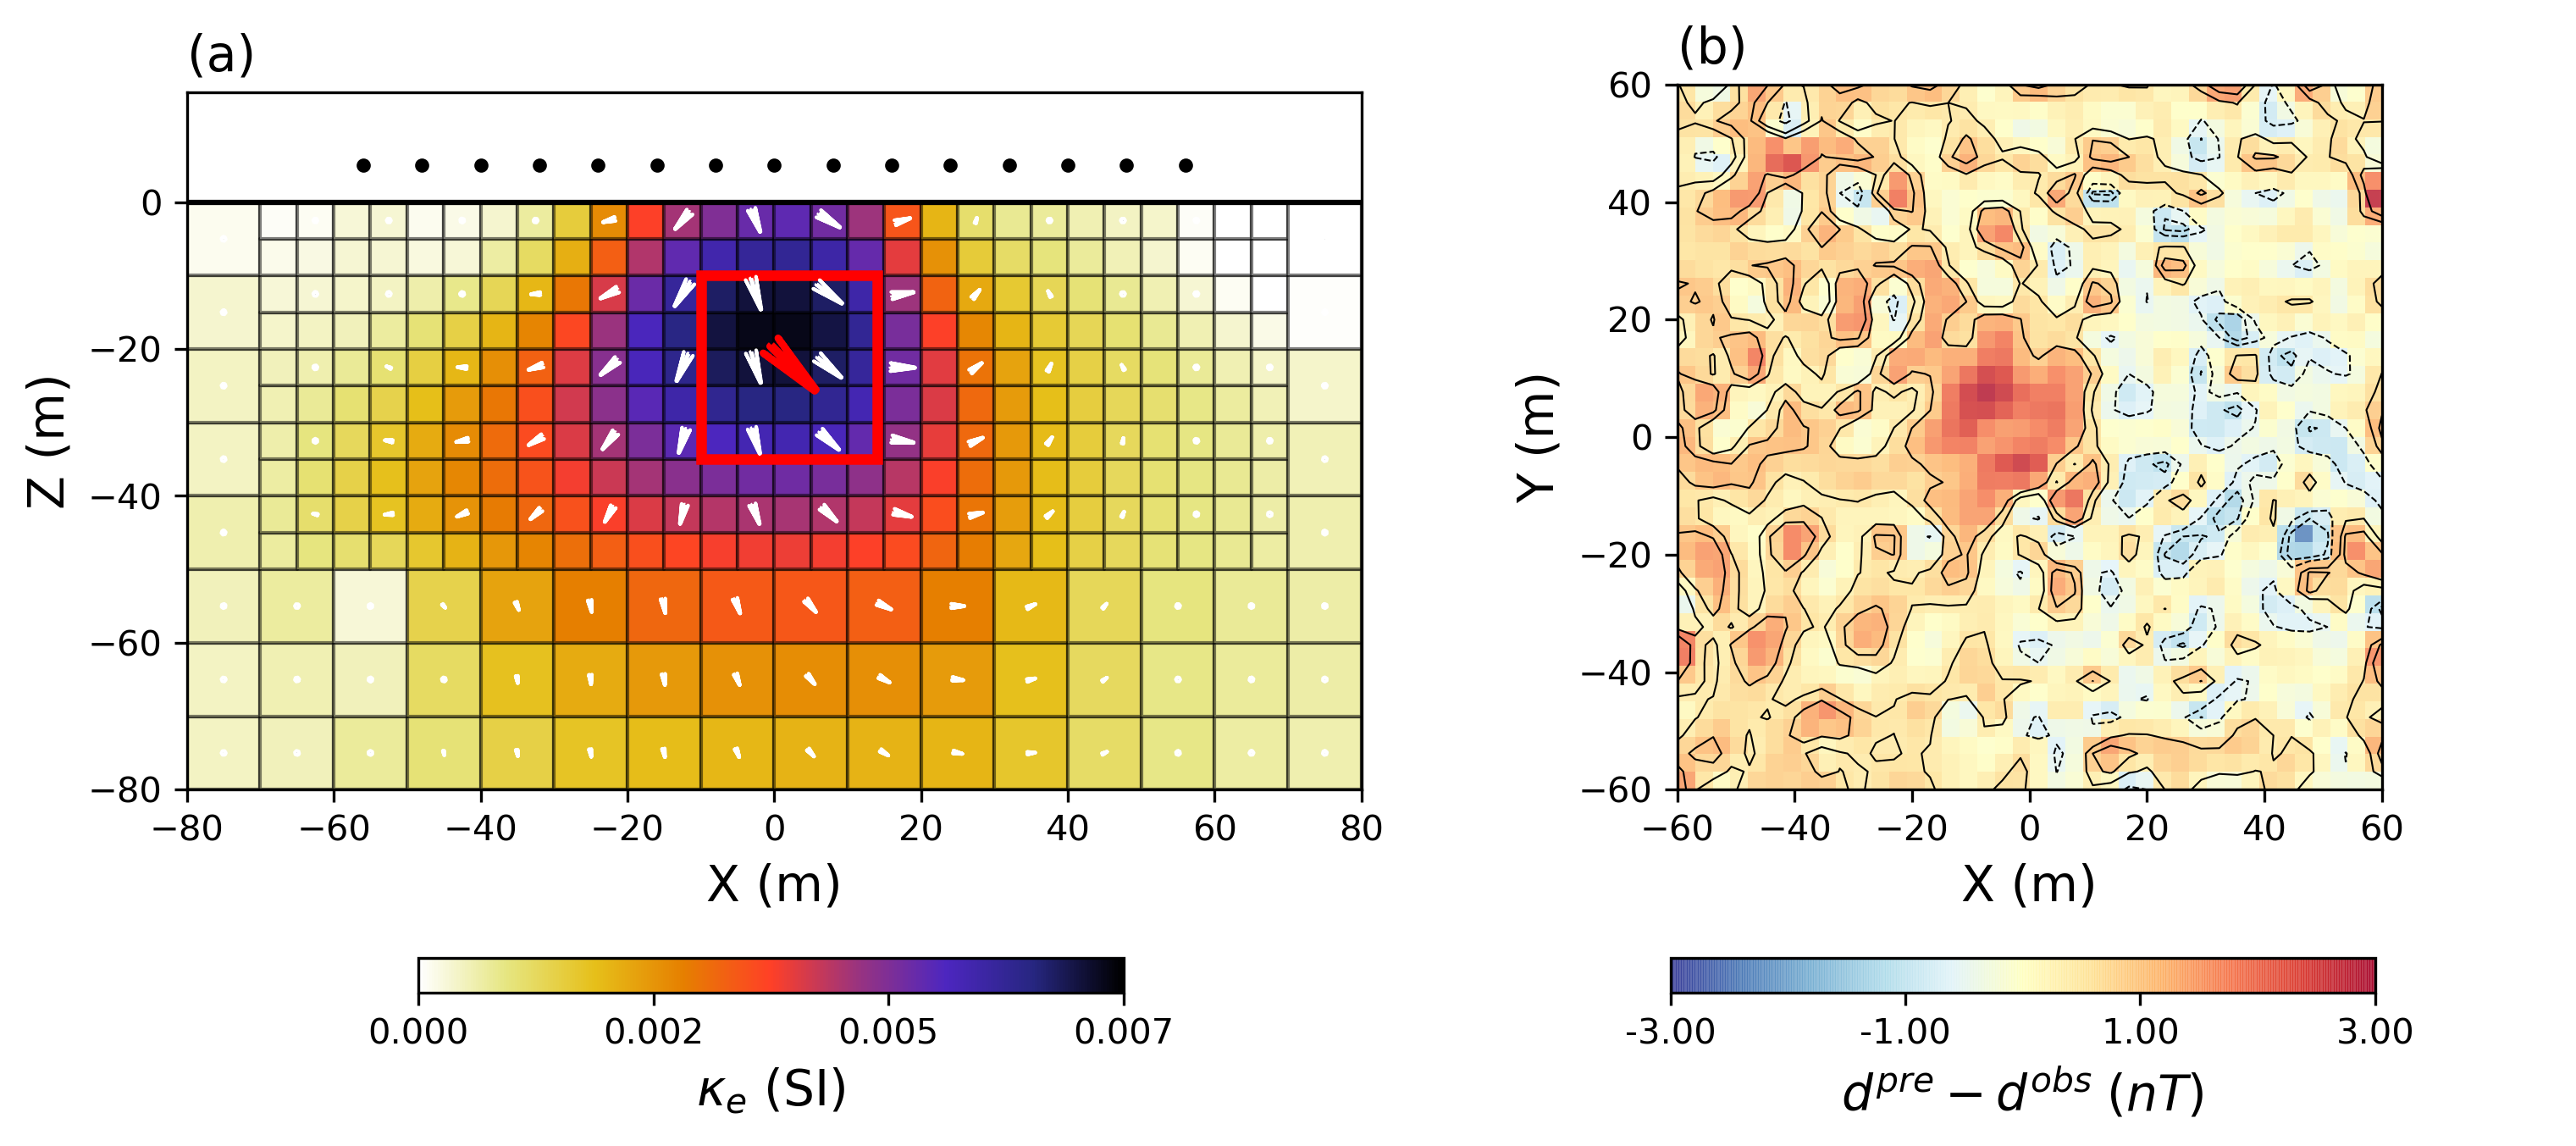
\includegraphics[width=\columnwidth]{Figures/Figure6.png}
\caption{(a) Vertical section through the recovered magnetization vector model in spherical coordinates using sensitivity based weighting and (b) the corresponding data residual map. The same poor starting model shown in Figure~\ref{MVI_S_model_noScale}a was used, but the algorithm converged to a solution similar to the Cartesian solution.}
\label{MVI_S_model}
\end{figure}

\begin{figure}[p!]
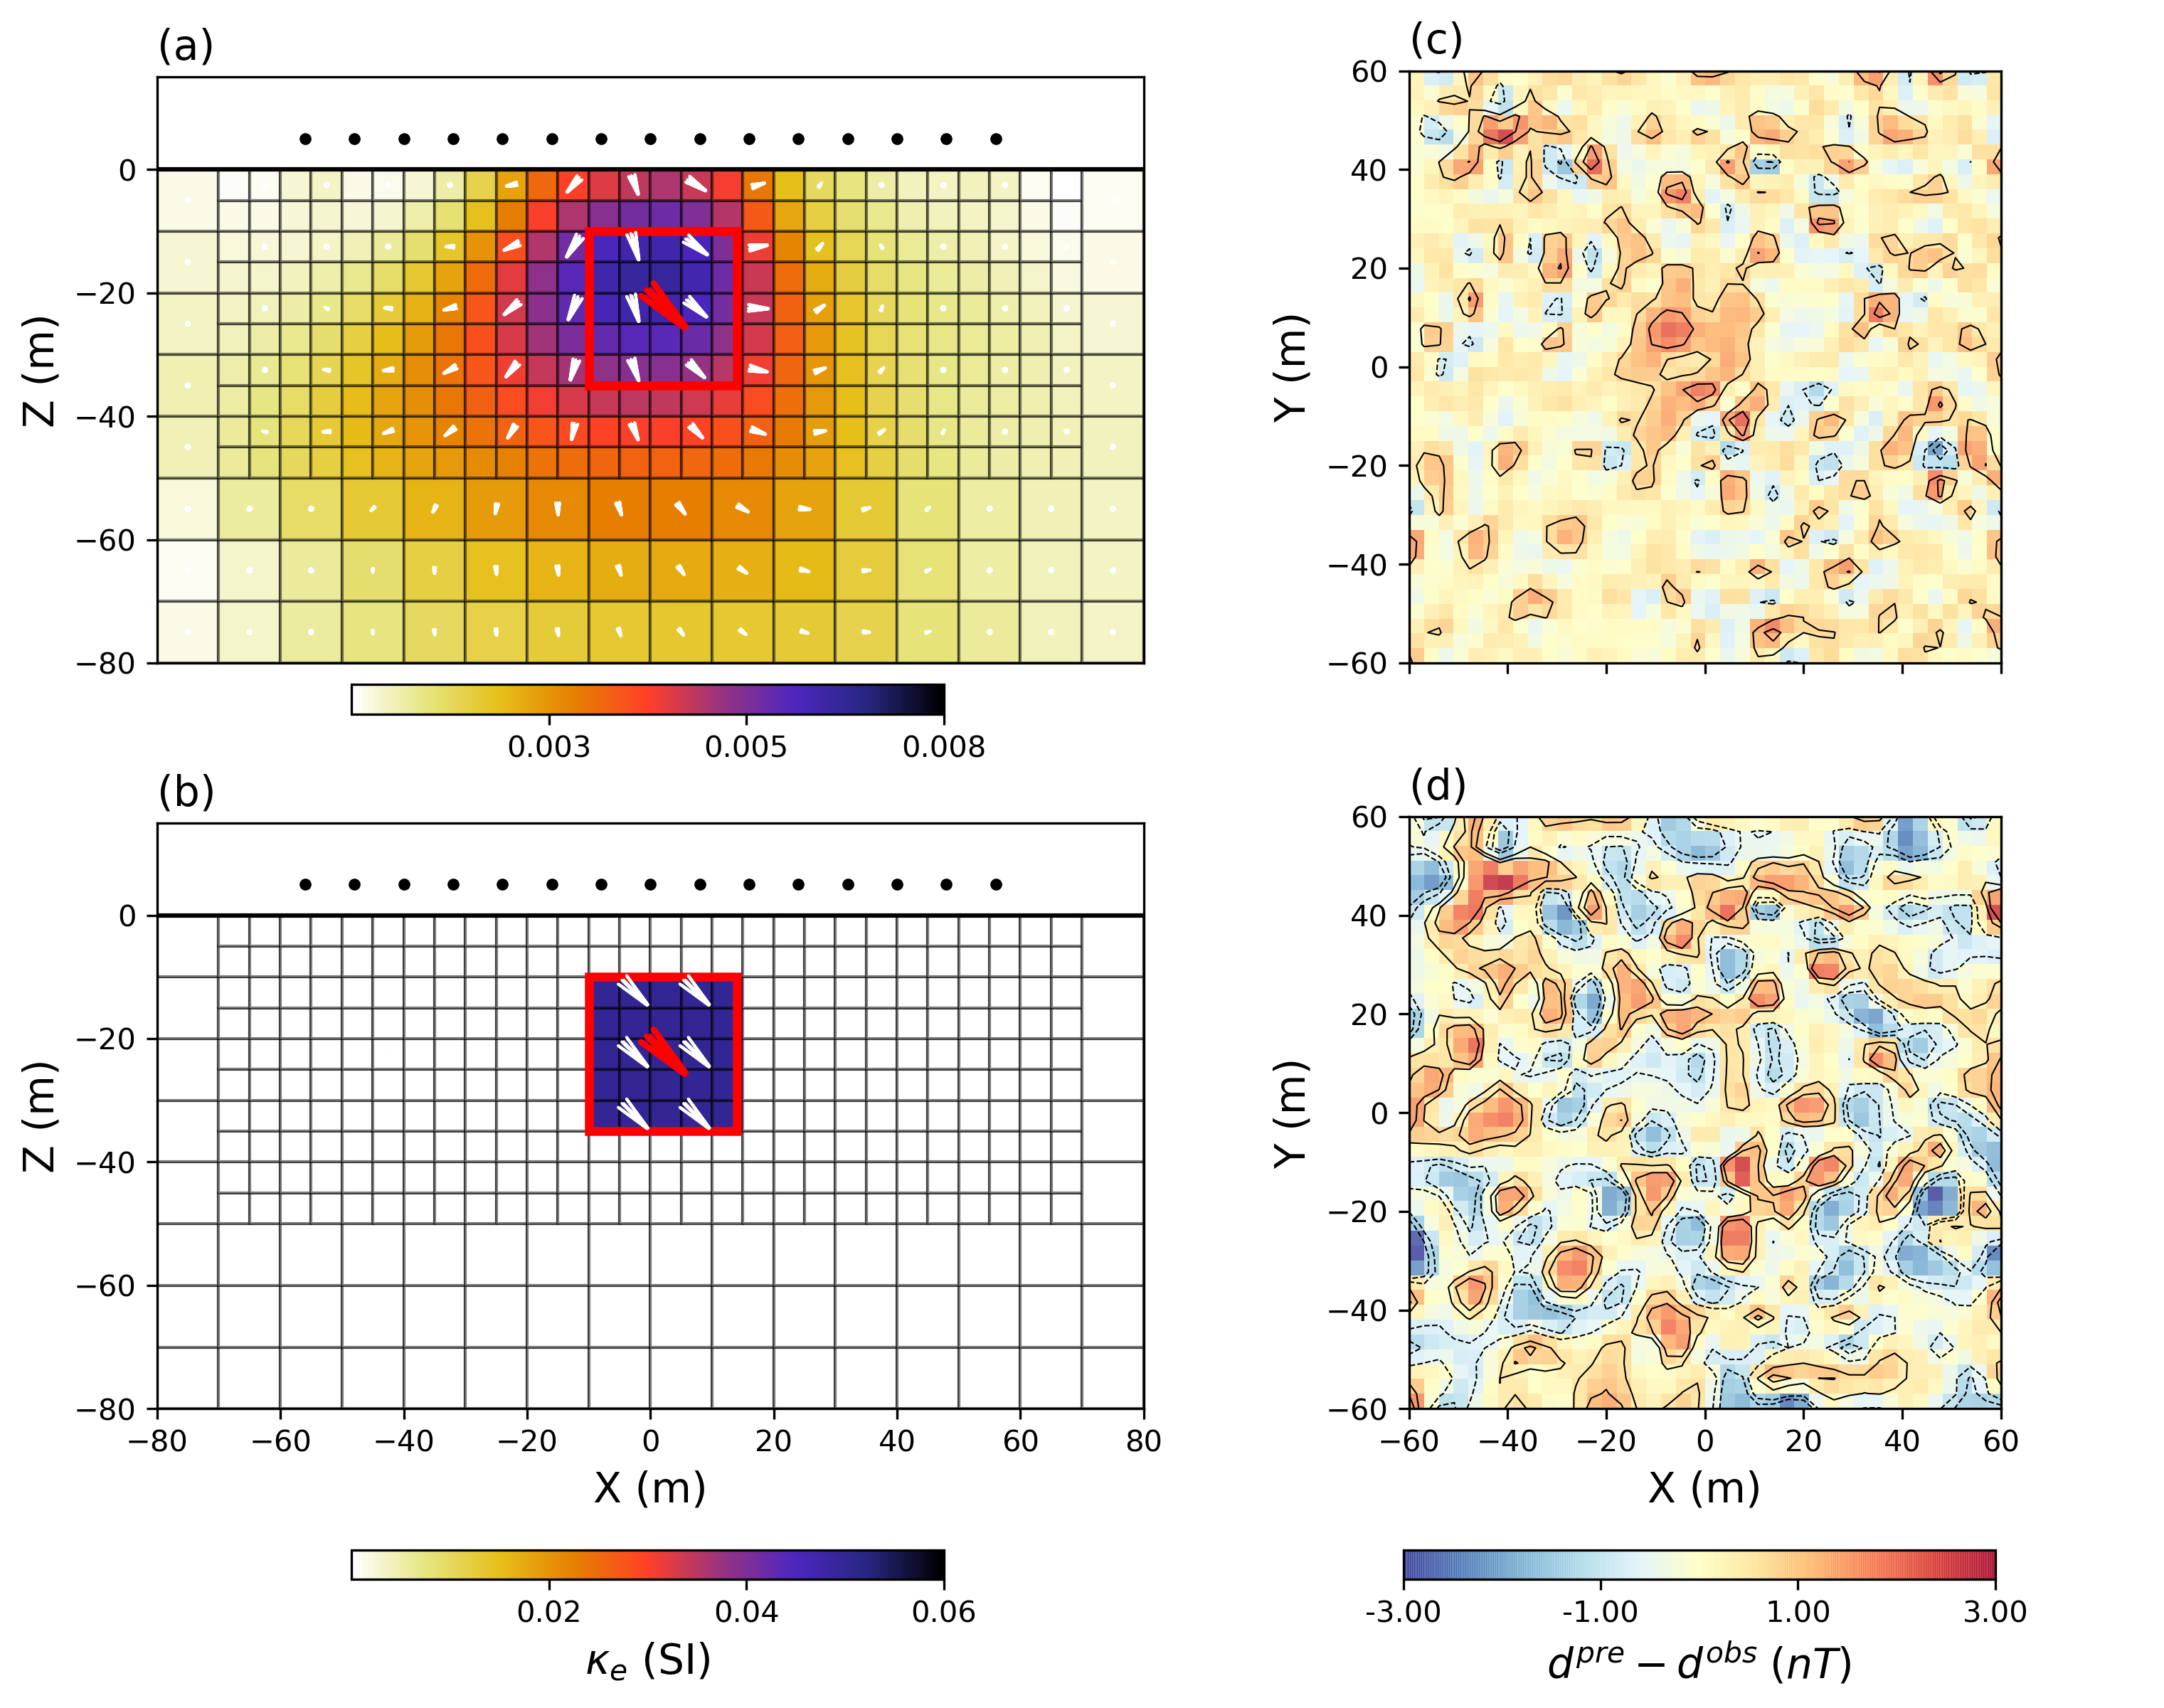
\includegraphics[width=\columnwidth]{Figures/Figure7.png}
\caption{Vertical section through the recovered magnetization vector model in spherical coordinates using sensitivity based weighting and the smooth Cartesian solution as starting model: (a) smooth regularization ($p_s=p_x=p_y=p_z = 2$) and (b) sparse norms on the strength and angles of the magnetization vector ($p_s=p_x=p_y=p_z = 0$). By using the sparse norms, we recover a solution that closely resembles the true model and, as observed in (d), we also eliminate the coherent signal in the residual data that is observed in (c).}
\label{MVI_S_model_lp}
\end{figure}

\begin{figure}[p!]
\includegraphics[width=\columnwidth]{Figures/Figure8.png}
\caption{(a) Geological map of the Kevitsa-Satovaara intrusive complex adapted from \cite{Koivisto2015}, with geological definition provided in Table~1. Mapped faults (dash) are shown for reference. (b) 2D seismic line reflection line E5 with interpreted geological contacts between the main reflectors.}
\label{Kevitsa_Geology}
\end{figure}

\begin{figure}[p!]
%\includegraphics[width=0.5\columnwidth]{Figure9.png}
\caption{Whisker plot of magnetic susceptibility measured along 279 boreholes. The coloured boxes have a width scaled by the calculated standard deviation and centered on the mean value for all intercepts belonging to the same lithological classification, as defined in Table~1. The black lines on either side define the minimum and maximum values. The different lithologies are colour coded and grouped based on relative age and similarities in physical properties.}
\label{Kevitsa_PhysProp}
\end{figure}

\begin{figure}[p!]
\includegraphics[width=\columnwidth]{Figures/Figure10.png}
\caption{Observed TMI data over the Kevitsa intrusion with histogram equalized color scale. Geological contacts (black), faults (dash) identified from surface mapping and the 2D seismic line locations E5, are shown for reference. Sun shading from east is added to highlight subtle features (Azimuth: $270^\circ$, Dip: $45^\circ$).}
\label{Kevitsa_TMI}
\end{figure}

\begin{figure}[p!]
\includegraphics[width=\columnwidth]{Figures/Figure11.png}
\caption{(a) Horizontal and (b) vertical sections through the recovered susceptibility model that ignores the effect of remanence. Lithological contacts (black) identified by \cite{Koivisto2015} are shown for reference. (c) The residual map shows strong correlation with the negative magnetic data.}
\label{MAG_lp_EW}
\end{figure}

\begin{figure}[p!]
\includegraphics[width=\columnwidth]{Figures/Figure12.png}
\caption{Horizontal sections at $\approx$ 300 m below topography for a suite of models using various sparsity assumptions put on the amplitude of magnetization for $p_s\;, p_{x,y,z} \in [0,\: 2]$. Norm measure on the magnetization angle are fixed to $p_{x,y,z}=0$ in order to promote uniform magnetization direction.}
\label{MVIS_Hsections}
\end{figure}

\begin{figure}[p!]
\includegraphics[width=\columnwidth]{Figures/Figure13.png}
\caption{Vertical sections along the E5 seismic reflection line for a suite of models using various sparsity assumptions put on the amplitude of magnetization for $p_s\;, p_{x,y,z} \in [0,\: 2]$. Norm measure on the magnetization angle are fixed to $p_{x,y,z}=0$ in order to promote uniform magnetization direction.}
\label{MVIS_Vsections}
\end{figure}

\begin{figure}[p!]
\includegraphics[width=\columnwidth]{Figures/Figure14.png}
\caption{Residual data maps for the nine inversions shown in Figure~\ref{MVIS_Hsections} and \ref{MVIS_Vsections}.}
\label{MVIS_predicted}
\end{figure}

\begin{figure}[p!]
\includegraphics[width=\columnwidth]{Figures/Figure15.png}
\caption{(a) Horizontal and (b) vertical sections through iso-contours of magnetization recovered from nine mixed $\ell_p$-norm inversions. Magnetization orientation (white arrowheads) and standard deviation on the angle (red arrowheads) are shown. (c) Data profile along the E5 section for the observed and predicted data calculated from the recovered models.}
\label{MVIS_Iso_model}
\end{figure}

\end{document}



\bibliography{references}
\bibliographystyle{seg}

%\listoffigures
% \pagebreak
%\listoftables

% \begin{table}
% \caption{Intervals along boreholes KV200 and KV297 reporting significant remanent magnetization.}
% \label{Table1}
% \end{table}

% \begin{table}
% \caption{Summary table grouping the various lithological units logged from boreholes. Expected magnetic susceptibility contrasts are derived from Figure~\ref{Kevitsa_PhysProp}.}
% \label{Table2}
% \end{table}

% \pagebreak

% \begin{figure}[p!]
% \includegraphics[width=\columnwidth]{Figures/Figure1.png}
% \caption{(a) Vertical section through the synthetic block model (Y = 0 m) with magnetization $\mathbf{M}$ [$2.0\: A/m,\; I: 45^\circ,\; D: 90^\circ$]($\kappa_e$ = 0.05 SI). Survey points (black dots) are placed 15 m above the magnetic anomaly. (b) Simulated TMI data map with random Gaussian noise added, 1 nT standard deviation. The horizontal position of the block is shown in black for reference.}
% \label{REM_model}
% \end{figure}

% \begin{figure}[p!]
% \includegraphics[width=\columnwidth]{Figures/Figure2.png}
% \caption{Vertical section through the recovered susceptibility model using (a) smooth assumption ($p_s, \;p_x,\; p_y,\; p_z = 2$) and (b) sparse $\ell_p$-norms to recover a compact model ($p_s,\;p_x,\; p_y,\; p_z = 0$). Both solutions show an anomaly with a false dip due to the wrong assumption of a vertical magnetization. Data residuals for (c) the smooth and (d) compact solution shows correlated signal with the negative data.}
% \label{Susc_model}
% \end{figure}

% \begin{figure}[p!]
% \includegraphics[width=\columnwidth]{Figures/Figure3.png}
% \caption{Vertical section through the recovered magnetization vector model using the Cartesian formulation with (a) smooth $l_2$-norm assumption and (b) sparsity constraints applied on all three Cartesian components ($p_{i_s}, \;p_{i_x},\; p_{i_y},\; p_{i_z} = 0$). Color is scaled by the magnitude of magnetization. The true magnetization direction is shown with a red arrow. Data residual map calculated with (c) the smooth and (d) compact solution.}
% \label{MVI_C_model}
% \end{figure}

% \begin{figure}[p!]
% \includegraphics[width=\columnwidth]{Figures/Figure4.png}
% \caption{ Vertical section through the (a) starting model and (b) recovered magnetization vector model in spherical coordinates with its (c) data residual map. The inversion stopped after three iterations, unable to further reduce the objective function.}
% \label{MVI_S_model_noScale}
% \end{figure}

% \begin{figure}[p!]
% \includegraphics[width=\columnwidth]{Figures/Figure5.png}
% \caption{Contour maps for the objective functions of a two-parameter inverse problem solved in (a) Cartesian and (b) polar coordinate systems. Solid colored lines show the model updates taken by different algorithms in their respective coordinate systems and, in dash, the equivalent steps in the other domain for comparison. Each inversion started with the same initial model (triangle). The colors and inversions are: Gray: the non-weighted Cartesian problem; Black: the sensitivity weighted Cartesian problem; Red: the non-linear polar coordinate system with fixed sensitivity weights; Green: the polar problem with iterative sensitivity re-weighting; and Blue: with the added scaling to compensate for the dynamic range of the parameters (see equation~50). }
% \label{NonLinearGN}
% \end{figure}

% \begin{figure}[p!]
% \includegraphics[width=\columnwidth]{Figures/Figure6.png}
% \caption{(a) Vertical section through the recovered magnetization vector model in spherical coordinates using sensitivity based weighting and (b) the corresponding data residual map. The same poor starting model shown in Figure~\ref{MVI_S_model_noScale}a was used, but the algorithm converged to a solution similar to the Cartesian solution.}
% \label{MVI_S_model}
% \end{figure}

% \begin{figure}[p!]
% \includegraphics[width=\columnwidth]{Figures/Figure7.png}
% \caption{Vertical section through the recovered magnetization vector model in spherical coordinates using sensitivity based weighting and the smooth Cartesian solution as starting model: (a) smooth regularization ($p_s=p_x=p_y=p_z = 2$) and (b) sparse norms on the strength and angles of the magnetization vector ($p_s=p_x=p_y=p_z = 0$). By using the sparse norms, we recover a solution that closely resembles the true model and, as observed in (d), we also eliminate the coherent signal in the residual data that is observed in (c).}
% \label{MVI_S_model_lp}
% \end{figure}

% \begin{figure}[p!]
% \includegraphics[width=\columnwidth]{Figures/Figure8.png}
% \caption{(a) Geological map of the Kevitsa-Satovaara intrusive complex adapted from \cite{Koivisto2015}, with geological definition provided in Table~1. Mapped faults (dash) are shown for reference. (b) 2D seismic line reflection line E5 with interpreted geological contacts between the main reflectors.}
% \label{Kevitsa_Geology}
% \end{figure}

% \begin{figure}[p!]
% %\includegraphics[width=0.5\columnwidth]{Figure9.png}
% \caption{Whisker plot of magnetic susceptibility measured along 279 boreholes. The coloured boxes have a width scaled by the calculated standard deviation and centered on the mean value for all intercepts belonging to the same lithological classification, as defined in Table~1. The black lines on either side define the minimum and maximum values. The different lithologies are colour coded and grouped based on relative age and similarities in physical properties.}
% \label{Kevitsa_PhysProp}
% \end{figure}

% \begin{figure}[p!]
% \includegraphics[width=\columnwidth]{Figures/Figure10.png}
% \caption{Observed TMI data over the Kevitsa intrusion with histogram equalized color scale. Geological contacts (black), faults (dash) identified from surface mapping and the 2D seismic line locations E5, are shown for reference. Sun shading from east is added to highlight subtle features (Azimuth: $270^\circ$, Dip: $45^\circ$).}
% \label{Kevitsa_TMI}
% \end{figure}

% \begin{figure}[p!]
% \includegraphics[width=\columnwidth]{Figures/Figure11.png}
% \caption{(a) Horizontal and (b) vertical sections through the recovered susceptibility model that ignores the effect of remanence. Lithological contacts (black) identified by \cite{Koivisto2015} are shown for reference. (c) The residual map shows strong correlation with the negative magnetic data.}
% \label{MAG_lp_EW}
% \end{figure}

% \begin{figure}[p!]
% \includegraphics[width=\columnwidth]{Figures/Figure12.png}
% \caption{Horizontal sections at $\approx$ 300 m below topography for a suite of models using various sparsity assumptions put on the amplitude of magnetization for $p_s\;, p_{x,y,z} \in [0,\: 2]$. Norm measure on the magnetization angle are fixed to $p_{x,y,z}=0$ in order to promote uniform magnetization direction.}
% \label{MVIS_Hsections}
% \end{figure}

% \begin{figure}[p!]
% \includegraphics[width=\columnwidth]{Figures/Figure13.png}
% \caption{Vertical sections along the E5 seismic reflection line for a suite of models using various sparsity assumptions put on the amplitude of magnetization for $p_s\;, p_{x,y,z} \in [0,\: 2]$. Norm measure on the magnetization angle are fixed to $p_{x,y,z}=0$ in order to promote uniform magnetization direction.}
% \label{MVIS_Vsections}
% \end{figure}

% \begin{figure}[p!]
% \includegraphics[width=\columnwidth]{Figures/Figure14.png}
% \caption{Residual data maps for the nine inversions shown in Figure~\ref{MVIS_Hsections} and \ref{MVIS_Vsections}.}
% \label{MVIS_predicted}
% \end{figure}

% \begin{figure}[p!]
% \includegraphics[width=\columnwidth]{Figures/Figure15.png}
% \caption{(a) Horizontal and (b) vertical sections through iso-contours of magnetization recovered from nine mixed $\ell_p$-norm inversions. Magnetization orientation (white arrowheads) and standard deviation on the angle (red arrowheads) are shown. (c) Data profile along the E5 section for the observed and predicted data calculated from the recovered models.}
% \label{MVIS_Iso_model}
% \end{figure}

\end{document}


